% Customizable fields and text areas start with % >> below.
% Lines starting with the comment character (%) are normally removed before release outside the collaboration, but not those comments ending lines

% svn info. These are modified by svn at checkout time.
% The last version of these macros found before the maketitle will be the one on the front page,
% so only the main file is tracked.
% Do not edit by hand!
\RCS$Revision: 315441 $
\RCS$HeadURL: svn+ssh://pakhotin@svn.cern.ch/reps/tdr2/notes/DN-13-022/trunk/DN-13-022.tex $
\RCS$Id: DN-13-022.tex 315441 2015-12-17 00:18:24Z pakhotin $
%%%%%%%%%%%%% local definitions %%%%%%%%%%%%%%%%%%%%%
% This allows for switching between one column and two column (cms@external) layouts
% The widths should  be modified for your particular figures. You'll need additional copies if you have more than one standard figure size.
\newlength\cmsFigWidth
\ifthenelse{\boolean{cms@external}}{\setlength\cmsFigWidth{0.85\columnwidth}}{\setlength\cmsFigWidth{0.4\textwidth}}
\ifthenelse{\boolean{cms@external}}{\providecommand{\cmsLeft}{top}}{\providecommand{\cmsLeft}{left}}
\ifthenelse{\boolean{cms@external}}{\providecommand{\cmsRight}{bottom}}{\providecommand{\cmsRight}{right}}
%%%%%%%%%%%%%%%  Title page %%%%%%%%%%%%%%%%%%%%%%%%
\cmsNoteHeader{DN-13-022} % This is over-written in the CMS environment: useful as preprint no. for export versions
% >> Title: please make sure that the non-TeX equivalent is in PDFTitle below
\title{ME1/1 Local Trigger Algorithm \\ for Operation under High Pile-Up Running Conditions}

% >> Authors
%Author is always "The CMS Collaboration" for PAS and papers, so author, etc, below will be ignored in those cases
%For multiple affiliations, create an address entry for the combination
%To mark authors as primary, use the \author* form
%\address[ghent]{Ghent University}
\address[tamu]{Texas A\&M University}
\address[ucla]{University of California, Los Angeles}
\address[ufl]{University of Florida}
\author[tamu]{Sven Dildick}
\author[tamu]{Jose Roberto Dimas Valle}
\author[tamu]{Jason Gilmore}
\author[ucla]{Jay Hauser}
\author[tamu]{Tao Huang}
\author[tamu]{Vadim Khotilovich}
\author[tamu]{Vyacheslav Krutelyov}
\author[ufl]{Alexander Madorsky}
\author[tamu]{Yuriy Pakhotin}
\author[ucla]{Andrew Peck}
\author[tamu]{Alexei Safonov}
\author[tamu]{Aysen Tatarinov}
\author[ucla]{Vyacheslav Valuev}

% >> Date
% The date is in yyyy/mm/dd format. Today has been
% redefined to match, but if the date needs to be fixed, please write it in this fashion.
% For papers and PAS, \today is taken as the date the head file (this one) was last modified according to svn: see the RCS Id string above.
% For the final version it is best to "touch" the head file to make sure it has the latest date.
\date{\today}

% >> Abstract
% Abstract processing:
% 1. **DO NOT use \include or \input** to include the abstract: our abstract extractor will not search through other files than this one.
% 2. **DO NOT use %**                  to comment out sections of the abstract: the extractor will still grab those lines (and they won't be comments any longer!).
% 3. For PASs: **DO NOT use tex macros**         in the abstract: CDS MathJax processor used on the abstract doesn't understand them _and_ will only look within $$. The abstracts for papers are hand formatted so macros are okay.
\abstract{
An important piece of the CMS muon trigger upgrade is developing and maintaining FPGA firmware for new custom electronics - optical trigger mother-board for ME1/1 muon detectors. This firmware uses massively parallel pattern recognition algorithm to find quality muon stubs. An improved local trigger algorithm to perform sophisticated background rejection is developed for operation under high pile-up running conditions. Implementation of the improvements to the algorithm is described. Configuration of the CMS software for the algorithm simulation is specified. Individual effects of the improvements on the ME1/1 local trigger efficiency are quantified and ranked using simulated samples.
}

% >> PDF Metadata
% Do not comment out the following hypersetup lines (metadata). They will disappear in NODRAFT mode and are needed by CDS.
% Also: make sure that the values of the metadata items are sensible and are in plain text:
% (1) no TeX! -- for \sqrt{s} use sqrt(s) -- this will show with extra quote marks in the draft version but is okay).
% (2) no %.
% (3) No curly braces {}.
\hypersetup{%
pdfauthor={Aysen Tatarinov, Yuriy Pakhotin},%
pdftitle={ME1/1 Local Trigger Algorithm for Operation under High Pile-Up Running Conditions},%
pdfsubject={CMS},%
pdfkeywords={LHC, CMS, Muons, CSC, Trigger}}

\maketitle %maketitle comes after all the front information has been supplied
% >> Text
%%%%%%%%%%%%%%%%%%%%%%%%%%%%%%%%  Begin text %%%%%%%%%%%%%%%%%%%%%%%%%%%%%
%% **DO NOT REMOVE THE BIBLIOGRAPHY** which is located before the appendix.
%% You can take the text between here and the bibiliography as an example which you should replace with the actual text of your document.
%% If you include other TeX files, be sure to use "\input{filename}" rather than "\input filename".
%% The latter works for you, but our parser looks for the braces and will break when uploading the document.

\tableofcontents

\newpage
\tracinginput{sections/sec_introduction.tex}
%\section{Introduction}

Muon system is hosted in the steel yokes of the CMS detector~\cite{Chatrchyan:2008aa} and it is divided into a central part (barrel: $|\eta| < 1.2$) with Drift-Tube (DT) detectors and two forward parts (endcaps: $0.9 < |\eta| < 2.4$) with Cathode Strip Chambers (CSC) as shown in Fig.~\ref{fig:CMS_muon_system}. Resistive Plate Chambers (RPC) are located in barrel and endcap parts ($|\eta| < 1.9$). The detectors of the muon system identify muons, provide a fast muon trigger, and give a precise measurement of the muon trajectory. Performance of the CMS muon system in LHC Run1 is described in~\cite{Chatrchyan:2013sba}.

\begin{figure}[b]
        \begin{center}
                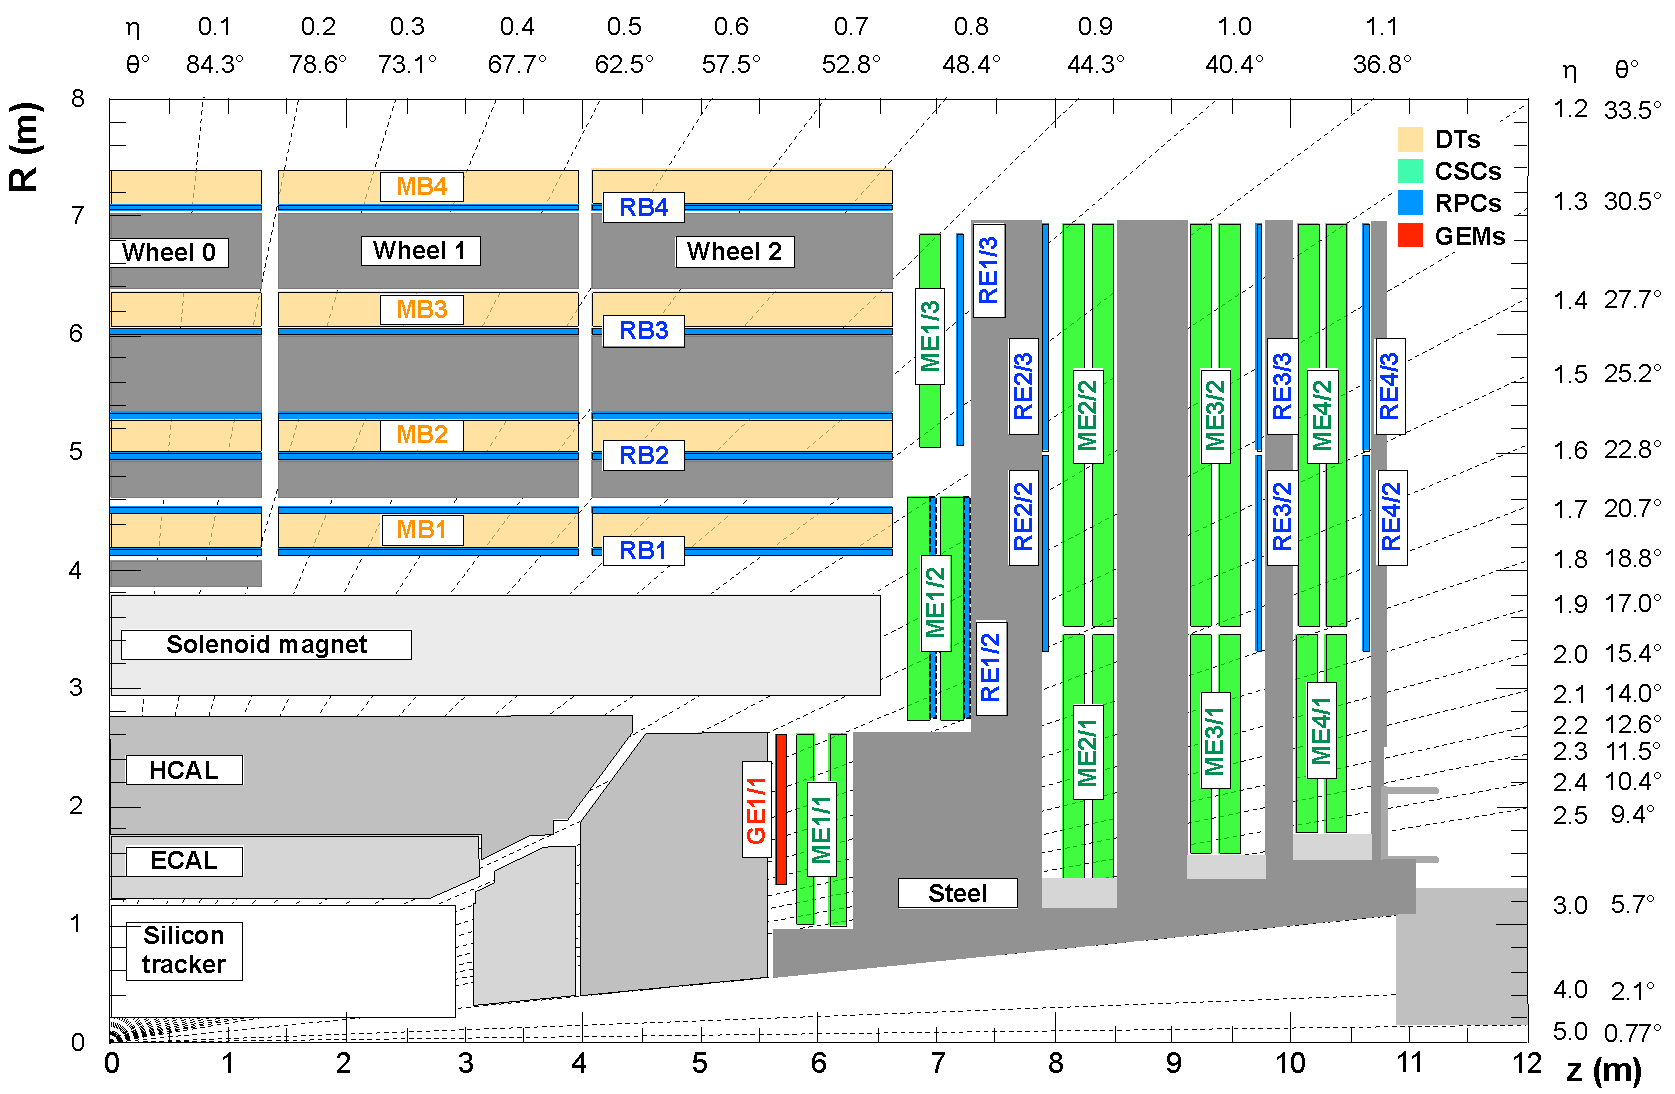
\includegraphics[width=0.99\linewidth]{figures/cms_upg_o_g_b_ni_ge11_r_grid_130919.pdf}
                \caption{Quarter-view of the CMS cross section. Detectors in the muon system are highlighted: DT -- orange, CSC -- green, RPC -- blue and future GE1/1 -- red.}
                \label{fig:CMS_muon_system}
        \end{center}
\end{figure}

The muon trigger is a tracking trigger that determines the momentum of muons using hits (position and angular measurements) in the muon system chambers situated in the magnetic field of the CMS detector. In this paper we describe several major improvements and upgrades to the muons system and their effect on the muon trigger performance. The focus of the muon trigger upgrade is to improve its rate reduction capability without significantly affecting the efficiency. We overview implementation of the muon trigger in endcaps in Section~\ref{sec:endcap_trigger}.

Installation of the outermost ring of CSCs in the fourth disk of each endcap (ME4/2) during 2013-2015 shutdown of the LHC (Long Shutdown 1 or LS1) allows to increase the number of muon hits along its trajectory. Major revision of the electronics for innermost ring of CSCs in the first disk (ME1/1) and unganging strips in the bottom part of these chambers allow to significantly enhance their performance in the trigger and in offline reconstruction. We describe details of the CSC upgrade during LS1 in Section~\ref{sec:csc_upgrade}.

New, robust and sophisticated, ME1/1 local trigger algorithm which is tolerant of the increased pile-up was also developed during LS1. Individual improvements of the upgraded algorithm are studied in details using simulation, and ranked in terms of their importance. The goal is to have improved ME1/1 local trigger algorithm commissioned during the 2015-16 Year-End Technical Stop (YETS), so that the upgraded trigger will be available to operate under high pile-up running conditions in 2016. Overview of the CSC local trigger algorithm is in Section~\ref{sec:csc_algo}. Specifics of the previous and upgraded algorithms implementation in electronics firmware, emulation in CMS software, as well as results of individual improvements are described in three sections:
\begin{enumerate}
\item anode signal processing (see Section~\ref{sec:alct}),
\item cathode signal processing (see Section~\ref{sec:clct}),
\item cathode-anode correlation (see Section~\ref{sec:lct}).
\end{enumerate}

As a part of future upgrade for Phase II of LHC running, the CMS will be equipped with Gas Electron Multiplier (GEM) detectors in the high pseudorapidity region ($1.5 < |\eta| < 2.2$) as shown in Fig.~\ref{fig:CMS_muon_system}. Pairs of triple-GEM chambers will be installed in the currently vacant position in front of the ME1/1 chambers and are dubbed GE1/1. The addition of such chambers allows to measure the bending angle of a track between GE1/1 and ME1/1. Usage of the bending angle at L1 can help to keep the rates down while having the efficiency high. Several implementation possibilities of the combined GEM-CSC local trigger algorithm for the high luminosity run of LHC are investigated in details in~\cite{CMS_DN-14-018}.
\clearpage

\newpage
\tracinginput{sections/sec_endcap_trigger.tex}
%\section{Muon Trigger in Endcaps}
\label{sec:endcap_trigger}

Each CSC can provide up to two local charged track (LCT) segments to the trigger logic per BX. These are formed in the trigger motherboard (TMB) combining cathode (CLCT) and anode (ALCT) segments. Present and improved logics of the algorithm which constructs LCTs are described in Section~\ref{sec:present_algo} and Section~\ref{sec:SLHC_algo}, respectively. The CLCT data contains information on the azimuthal position of the segment ($\phi$), the bend angle, and the pattern of cathode half-strips with hits in a chamber. The ALCT data contains information on the radial position from the beamline of the segment (equivalent to $\eta$), and the pattern of anode wires with hits in a chamber. The timing information from anodes is used to define the time of the combined LCT. There is one TMB per CSC, located in a crate on the periphery of the detector. The TMB sends up to two LCTs over a custom backplane to the muon port card (MPC), which is located in the same peripheral crate. One MPC can receive data from up to 9 TMBs, or equivalently, can receive up to 18 LCTs. The LCTs in a MPC are sorted by rank (see definition in MPC documentation). The best three LCTs are sent over optical fibers to the CSCTF. There are a total of sixty peripheral crates for the CSC system, each with one MPC.

The CSCTF system is partitioned into sectors, each of which corresponds to a $60^{o}$ azimuthal region of an endcap. Twelve ``sector processors'' are required for the entire endcap muon system, six per endcap. Each sector processor is a 9U VME card that is housed in a single crate. Three 1.6 Gb/s optical links from each of five MPCs are received by each sector processor, for a total of 180 optical links for the entire system. The CSCTF sectors are independent, since there is no sharing of data across boundaries of neighboring sectors, leading to slight inefficiencies.

There are several Field Programmable Gate Arrays (FPGAs) on each ``sector processor'', but the main FPGA for the track-finding algorithms is from the Xilinx Virtex-5 family. The conversion of strip and wire positions of each track segment to ($\eta, \phi$) coordinates is accomplished via a set of cascaded SRAM look-up tables (LUTs), each $512K\times16$ bits. These coordinates are then used for track-finding and momentum assignment.

The CSCTF track-finding logic consists of pairwise comparisons of track segments in different detector stations. These test for compatibility in $\phi$ and $\eta$ with a muon emanating from the collision vertex within certain tolerance windows. The comparisons are then analyzed and built into tracks consisting of possibly more than two segments from different stations. Possible duplicate (?ghost?) tracks are canceled. The track-finding logic has the ability to accept segments in different assigned bunch crossings by analyzing across a sliding time window of programmable length (nominally 2 BX) every bunch crossing. Duplicate tracks found on consecutive bunch crossings are canceled. The bunch crossing of a track is given by the second arriving track segment.

The $p_T$ of a muon candidate is calculated by using a large LUT implemented in SRAM. Information such as the track type, track $\eta$, the segment $\phi$ differences between a maximum of 3 stations, and the segment bend angle in the first measurement station are used to calculate the LUT address.

In addition to identifying muons from proton collisions, the CSCTF processors also simultaneously identifies any beam halo muons for monitoring and veto purposes by looking for trajectories approximately parallel to the beam line.

Each CSCTF sends up to three muon candidates per bunch crossing over a custom backplane to a muon sorter (MS). The MS then sorts the candidates by momentum and quality and selects the best 4 for the GMT. The CSCTF data are also sent to a DAQ card with SLINK interface which puts the trigger data into the event record.

\clearpage

\newpage
\tracinginput{sections/sec_endcap_upgrade.tex}
%\section{Endcap Muon System Upgrade}
\label{sec:csc_upgrade}

All CSCs in ME4/2 rings have been installed during LS1. This results in four measurement stations for muons in the region $1.25 < |\eta| < 1.8$ providing additional redundancy in a high rate environment. This redundancy is especially important for future upgraded Global Muon Trigger (GMT) algorithms. For the CSC Track Finder (TF) additional measurement in this region will increase the efficiency and improve the rate reduction since it will be more likely to have 3 or more hits used in the $p_T$ assignment logic. No additional hardware or reconfiguration of the present muon trigger was required after this upgrade. The muon sector receiver boards for the fourth disk already were in place and the present CSCTF already had logic to process trigger data from these chambers.

Electronics for the CSCs have been also under major revision during LS1. All CSCs in ME1/1 rings received new digital cathode front-end boards (DCFEB) as well as new optical trigger motherboards (OTMB) and optical data acquisition motherboars (ODMB) as schematically shown in Fig.~\ref{fig:me11_upgrade_overview}. The new electronics will significantly enhance ME1/1 performance in the trigger and in the offline reconstruction providing a key sagitta measurement for the muon L1 trigger in the region $1.6 < |\eta| < 2.4$. The recovered old electronic boards were used to instrument the newly installed ME4/2 chambers.

The strips of the ME1/1 chambers are split into two regions at $|\eta| = 2.1$ (see details on mechanical layout and signal readout of the ME1/1 chambers in Appendix~\ref{app:me11}). The bottom region ($2.1 < |\eta| < 2.4$) previously had 48 strips triple-ganged to 16 channels in the electronics for both the trigger and the readout, making hit recognition ambiguous. The ambiguity can be mitigated using measurements from the outer stations. However, the $p_T$ resolution using only the outer stations is quite coarse, leading to a significantly increased single muon trigger rate in the forward region $2.1<|\eta|<2.4$. As a result, this region generated a single muon trigger rate comparable to that of the entire region $|\eta| < 2.1$. With the new seven DCFEBs per chamber, this triple-ganging is removed, leading to improved triggering performance in the forward region which allows to maintain highly efficient muon trigger coverage up to $|\eta| = 2.4$.

\begin{figure}[b]
        \begin{center}
                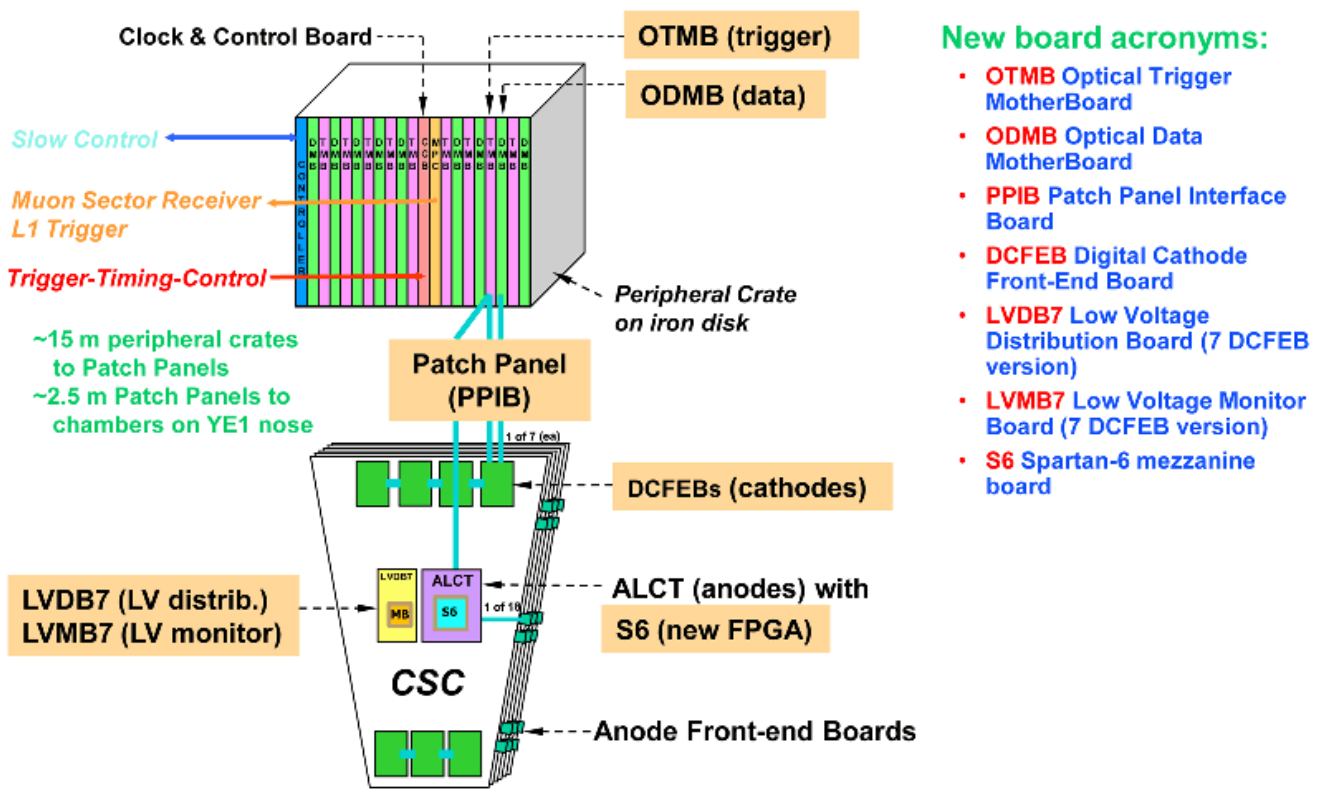
\includegraphics[width=0.85\linewidth]{figures/ME11_upgrade_overview.png}
                \caption{Schematic overview of the ME1/1 electronics upgrade after LS1.}
                \label{fig:me11_upgrade_overview}
        \end{center}
\end{figure}
\clearpage

\newpage
\tracinginput{sections/sec_algorithm.tex}
%\section{Overview of the CSC Local Trigger Algorithms}
\label{sec:csc_algo}

An improved ME1/1 local trigger algorithm to perform sophisticated background rejection is developed for operation under high pile-up running conditions.

\subsection{Results of Improvements in the ME1/1 Local Trigger Algorithm}
\label{sec:SLHC_algo_results}

This chapter presents results of the study of effects of individual improvements described in Sec.~\ref{sec:SLHC_algo} on the ALCT, CLCT, and LCT reconstruction efficiencies.

The study is performed with Monte Carlo simulation of double muon events mixed with PU400 events, where the simulation includes GEN, SIM, DIGI, L1 steps.

Three are three baseline configurations of L1 step used in this study:
\begin{itemize}
	\item Baseline 1: SLHC configuration, where the maximum set of improvements is turned off bringing it to 2007 configuration as close as possible. 
	There are only two differences between Baseline 1 and 2007 configurations: separate treatments of ME1/1a and ME1/1b, and unganging cathode strips in ME1/1a;
	\item Baseline 2: Baseline 1 configuration with all improvements on the ALCT and CLCT processors level turned on;
	\item Baseline SLHC: best CSC4 configuration itself.
\end{itemize}

All algorithm improvements divided into three groups and studied with improvements in the given group turned on one by one on top of each other
\begin{itemize}
	\item ALCT processor level
	\item CLCT processor level
	\item TMB level
\end{itemize}

In the first two groups the L1 step configuration gradually changes from Baseline 1 to Baseline 2 configuration, in the last one --- from Baseline 2 to SLHC configuration.
\clearpage

\newpage
\tracinginput{sections/sec_algorithm_alct.tex}
%\section{Anode Signal Processing}
\label{sec:alct}

\subsection{ALCT Algorithm}
\label{subsec:alct_algo}

Anode wires in CSC are hardwired together at the readout end in groups of 10-15 wires in order to reduce channel count. The anode wire group (WG) signals are fed into the anode front-end boards (AFEBs), each of which contains a single 16-channel amplifier/constant-fraction discriminator chip. The output signals from the AFEBs are sent into the on-chamber ALCT board, which handles triggering and readout of the CSC anode information. Due to the various sizes of CSCs, there are 3 types of ALCT boards, handling 288, 384, and 672 WG channels.

On the ALCT boards, the signals from each AFEB are first delayed by a programmable amount of time in order to perform an average time alignment of the anode signals across the chamber as well as chamber-to-chamber at a sub-bunch crossing level to about 2.2 ns precision. After the AFEB signals are received and time-aligned, then they are latched with bunch crossing frequency and fed to a FPGA (Xilinx Virtex family) mounted on a mezzanine card above the ALCT main board for pattern-finding and readout functions.

The algorithm used in the ALCT FPGA for determining muon segment position and bunch crossing is illustrated below. Since the drift time can be longer than 50 ns, the hits are first stretched by 'one-shots' to 6 BX (150 ns) length. Then, a multi-layer coincidence technique in the ALCT pattern circuitry is used to identify the bunch crossing. For each spatial pattern of anode hits, a low coincidence level, typically 2 or more layers, is used to establish timing, whereas a higher coincidence level, typically 4 layers, is used to establish the existence of a muon track. The general idea of a spatial pattern of CSC wire group hits is illustrated below in Fig.\ref{fig:anode_wire_group_hits}.

\begin{figure}[tbh]
        \begin{center}
                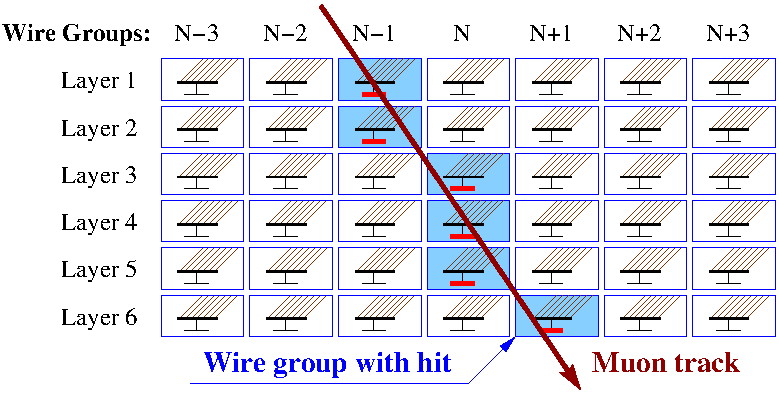
\includegraphics[width=0.6\linewidth]{figures/anode_wire_group_hits.pdf}
                \caption{Illustration of CSC anode wire groups with hits from muon track}
                \label{fig:anode_wire_group_hits}
        \end{center}
\end{figure}

while the general idea of the time stretching of hits, and pretrigger followed by a pattern trigger is shown in Fig.\ref{fig:anode_stretched_hits} (using an example in which one hit is actually missing due to some type of inefficiency).

\begin{figure}[tbh]
        \begin{center}
                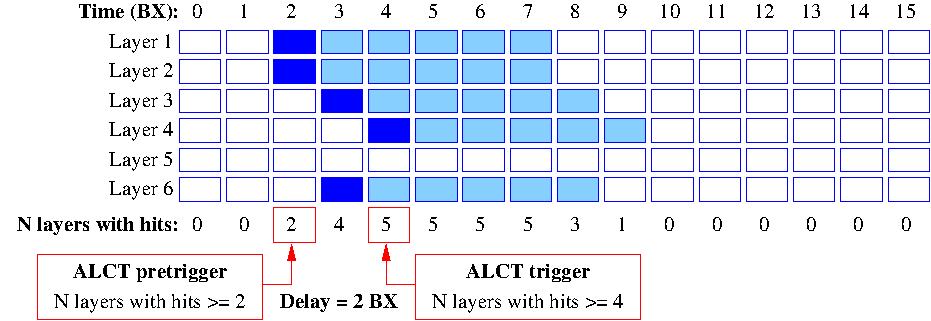
\includegraphics{figures/anode_stretched_hits.pdf}
                \caption{Illustration of anode hits time stretching (6BX) as well as determination of ALCT pretrigger and trigger.}
                \label{fig:anode_stretched_hits}
        \end{center}
\end{figure}

Each pattern detector can detect a programmable "collision" pattern as well as a fixed "accelerator" pattern. The input data for the collision pattern detector are selected as shown below:

\begin{center}
\begin{verbatim}
...n-2 n-1 n...........Layer 1
.......n-1 n...........Layer 2
...........n...........Layer 3
...........n n+1.......Layer 4
...........n n+1 n+2...Layer 5
...........n n+1 n+2...Layer 6
\end{verbatim}
\end{center}

where n in this diagram is the key wire group number, which this particular pattern detector is searching the patterns for. The programming of the programmable collision pattern is implemented as a simple masking-out of the bits that we do not want to include in the pattern. The accelerator pattern is a vertical pattern of 6 layers all with strip n only.

Each ALCT candidate is assigned a quality equal to number of layers with hits minus 3 and passes through a ghost cancellation procedure: it is cancelled if there is another ALCT candidate at the same bunch crossing in the previous wirewith the same or better quality or in the next wire with better quality, or if there is ALCT candidate up to 4 bunch crossing clocks earlier with any quality.

In each bunch crossing two ALCTs with highest quality are sent to the TMB (Trigger MotherBoard), which requires a coincidence between anode and cathode trigger information. In the case of a Level-1 Accept signal from the Global Trigger (distributed via the TTC system to the CCB in each peripheral crate), ALCT data are sequentially transmitted to the Trigger Mother Board and hence to the DAQ Motherboard. These data frames include a few words of ALCT trigger data and a much larger amount of ALCT raw hit data consisting of a time sequence of raw CSC anode wire-group hits that have been stored at the 40 MHz bunch crossing frequence by the ALCT2001. Typically 8 to 16 bunch crossings are read out for each wire group. FIFO data can also be read out much more slowly through VME access via the TMB board using a JTAG electrical interface to the ALCT, if necessary.

For self-monitoring and also for powering and controlling the AFEB cards, the ALCT contains a Slow Control section that supplies power to the AFEBs, controls AFEB thresholds, provides and controls the amplitude of test pulses to the AFEBs, and reads back power supply voltages and currents, as well as on-board temperature. 

\subsection{Improvement of the ALCT Algorithm}
\label{subsec:alct_improvements}

It should be possible to improve the efficiency, rate and timing precision of ALCT stubs by, e.g.
\begin{itemize}
    \item tuning of the ghost cancellation logic (ALCTs in neighboring wiregroups, see "alctGhostCancellationBxDepth" and "alctGhostCancellationSideQuality" parameters in Sec.~\ref{sec:ALCT_conf}) and removing pre-trigger deadtime (see "alctPretrigDeadtime" parameter in Sec.~\ref{sec:ALCT_conf});
    \item using more narrow ALCT pattern in ring 1 chambers (see "alctNarrowMaskForR1" parameter in Sec.~\ref{sec:ALCT_conf});
    \item using more precise algorithm (e.g., running median or truncated average) for BX assignment (see "alctUseCorrectedBx"  parameter in Sec.~\ref{sec:ALCT_conf}).
\end{itemize}

However, here we would only like to focus on how the ALCT stubs would be used by TMB.

ALCTs are reconstructed from the signals in layers of anode wires which are ganged into wiregroups and are continuously covering the whole ME1/1 chamber. Most of the wiregroups can only physically cross only strips either in ME1/1a or only in ME1/1b. A complication specific to ME1/1 is that wires here are not perpendicular to strips, but are slanted at 29 degrees from the straight angle. Thus, some wiregroups are crossing the border between ME1/1a and ME1/1b. If signal is detercted in such a wiregroup, there is an ambiguity about which part of ME1/1 it might belong to.

For the ALCTs received by TMB we propose to split the incoming stubs into two parts, ME1/1a and ME1/1b, that would be used further for LCT matching separately in ME1/1a and ME1/1b. 




\subsection{Emulation of ALCT Algorithm}
\label{subsec:alct_emulation}

ALCT processing includes the following five steps:

\begin{itemize}
    \item Pulse extension;
    \item Pretrigger;
    \item Trigger;
    \item Ghost cancellation;
    \item ALCT construction.
\end{itemize}

\subsubsection{Pulse Extension}

Sofware emulation provides information about all wire signals in DAQ readout window (16 BXs). A search for these signals is performed in a loop over all wire groups, all layers, and all 16 BXs; found signals are stretched over 6 BXs (see Fig.~\ref{fig:alct_pulse_extension}).

\begin{figure}[tbh]
        \begin{center}
                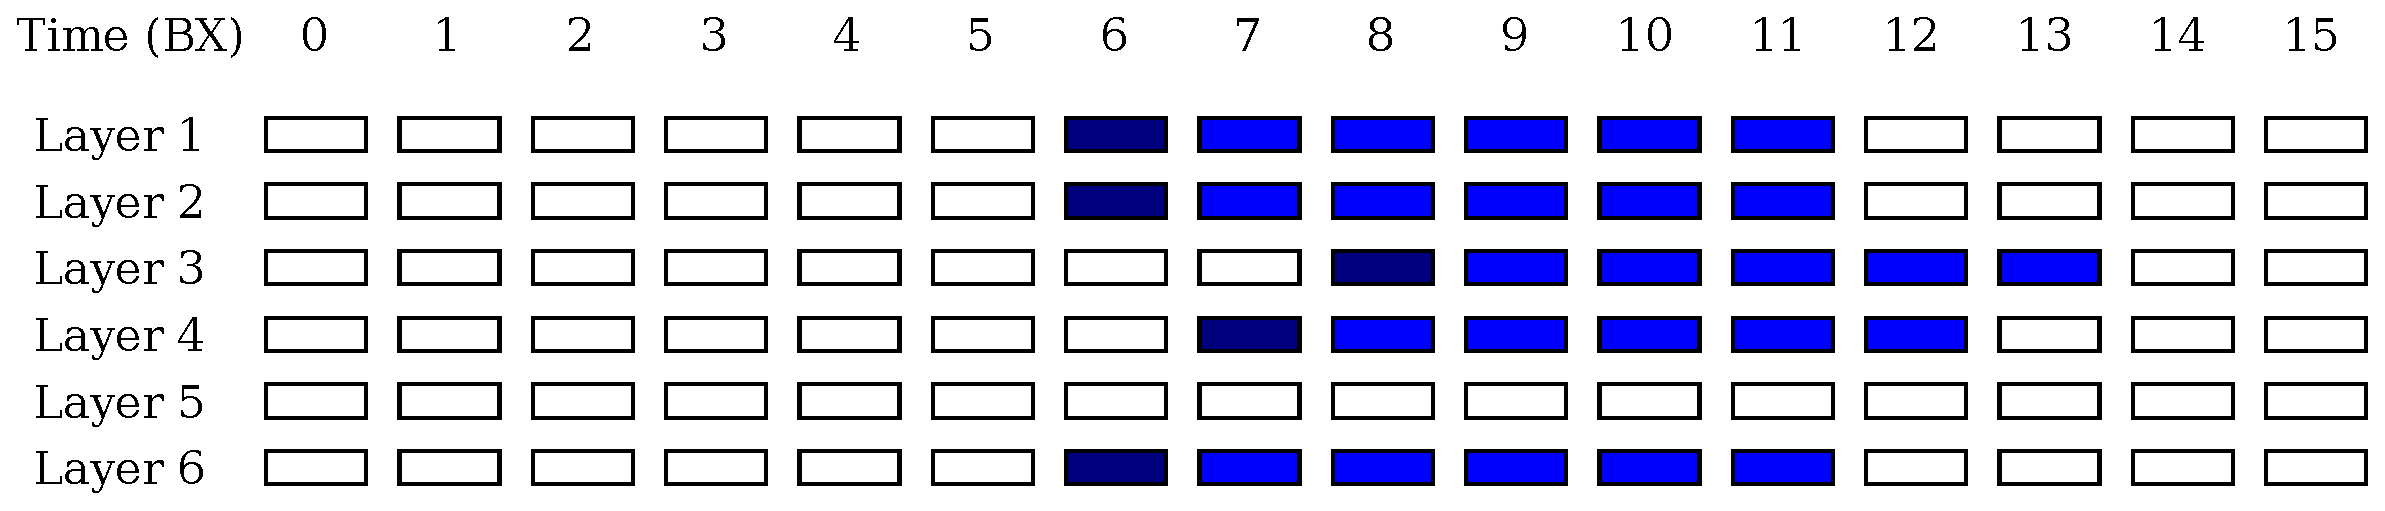
\includegraphics[width=0.9\linewidth]{figures/stretched_hits_alct.pdf}
                \caption{Illustration of ALCT pulse extension for one specific wire group.}
                \label{fig:alct_pulse_extension}
        \end{center}
\end{figure}

\subsubsection{Pretrigger}

After all available wire signals are stretched, a search for ALCT pretriggers is performed in all wire groups and all BXs. For any given wire group and BX, we count the number of layers with hits within the pattern mask shown on Fig.~\ref{fig:alct_pretrigger}, and if this number is greater than or equal to three, then we say that a pretrigger occured in this wire group and BX. The search for next ALCT pretrigger starts 6 BXs later.

\begin{figure}[tbh]
        \begin{center}
                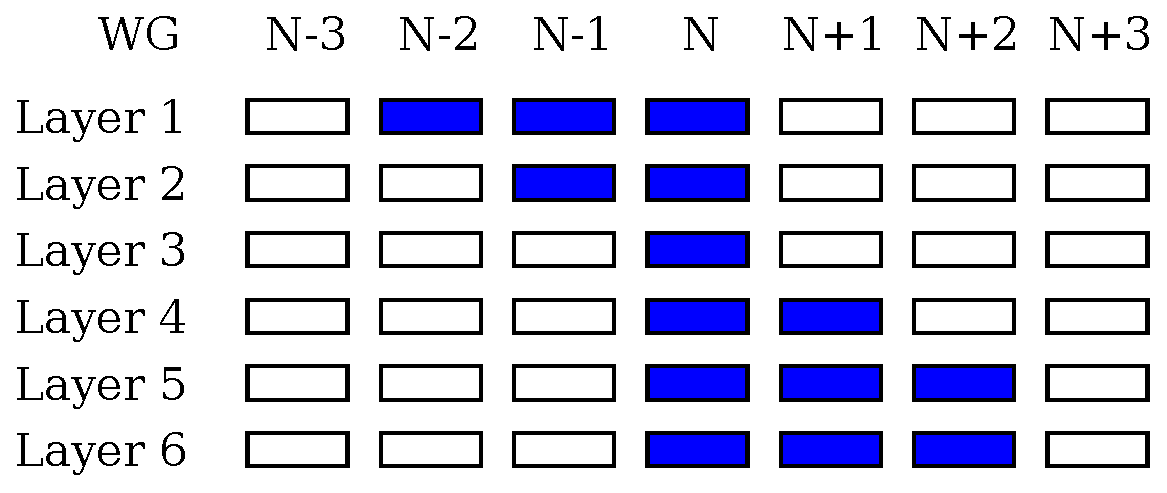
\includegraphics[width=0.45\linewidth]{figures/alct_pretrigger.pdf}
                \caption{ALCT pattern mask for pretriggering and triggering.}
                \label{fig:alct_pretrigger}
        \end{center}
\end{figure}

\subsubsection{Trigger}

After all ALCT pretriggers are found, for each pretrigger in BX = B we check for a trigger in BX = B+2. For any given wire group and BX = B+2, we count the number of layers with hits within the same pattern mask used for pretriggering, and if this number is greater than or equal to four, we say that a pretrigger occured in this wire group and BX, and assign it a quality Q = number of layers with hits-3. If in some wire group more than one trigger occured, we report only the one with the highest quality. If there are two triggers with the same quality, report the earlier one.

\subsubsection{Ghost Cancellation}

Not all triggers found in the previous step are used to construct ALCTs: before that all of them pass through so called ghost cancellation procedure.

A trigger in wire group = N and BX = B is cancelled if there is a trigger in wire group = N-1:
\begin{itemize}
    \item either in the same BX = B and with better or equal quality;
    \item or to 4 BXs earlier, with any quality.
\end{itemize}

In addition, a trigger in wire group = N and BX = B is cancelled if there is a trigger in wire group = N+1:
\begin{itemize}
    \item either in the same BX = B and with better quality;
    \item or to 4 BXs earlier, with any quality.
\end{itemize}

\subsubsection{ALCT Construction}

Construct ALCTs from triggers survived after the ghost cancellation procedure: encode quality, WG, BX (defined by pretrigger BX). In every BX choose best two ALCTs: two ALCTs with the highest quality. If we need to choose one ALCT from two ALCTs with the same quality: choose the one with larger wire group.


\subsection{Sofware Emulation of ALCT Level Improvements}

\subsubsection{Tuning of Ghost Cancellation Procedure}

\textcolor{red}{Current} ghost cancellation:
\begin{itemize}
    \item Loop over wire groups:
    \begin{itemize}
        \item Consider WG = N
        \item Cancel trigger in this wire group if there is trigger in WG = N-1 and:
        \begin{itemize}
            \item with the same BX and with \textcolor{red}{better or equal} quality
            \item up to \textcolor{red}{4} BXs earlier, with \textcolor{red}{any} quality
        \end{itemize}
        \item Cancel trigger in this wire group if there is trigger in WG = N+1 and:
        \begin{itemize}
            \item with the same BX and with \textcolor{red}{better} quality
            \item up to \textcolor{red}{4} BXs earlier, with \textcolor{red}{any} quality
        \end{itemize}
    \end{itemize}
\end{itemize}
\textcolor{blue}{New} ghost cancellation:
\begin{itemize}
    \item Loop over wire groups:
    \begin{itemize}
        \item Consider WG = N
        \item Cancel trigger in this wire group if there is trigger in WG = N-1 and:
        \begin{itemize}
            \item with the same BX and with \textcolor{blue}{better} quality
            \item up to \textcolor{blue}{1} BX earlier, with \textcolor{blue}{better} quality
        \end{itemize}
        \item Cancel trigger in this wire group if there is trigger in WG = N+1 and:
        \begin{itemize}
            \item with the same BX and with \textcolor{blue}{better or equal} quality
            \item up to \textcolor{blue}{1} BX earlier, with \textcolor{blue}{better and equal} quality
        \end{itemize}
    \end{itemize}
\end{itemize}

The following modifications in configuration are related to this improvement:
\begin{itemize}
    \item alctGhostCancellationBxDepth: 4BX to 1BX
    \item alctGhostCancellationSideQuality: False to True
\end{itemize}

\subsubsection{Narrow ALCT Pattern Mask}

Use more narrow ALCT pattern mask for stations in Ring 1 (see Fig.~\ref{fig:narrow_alct_pattern_mask}).

\begin{figure}[tbh]
        \begin{center}
                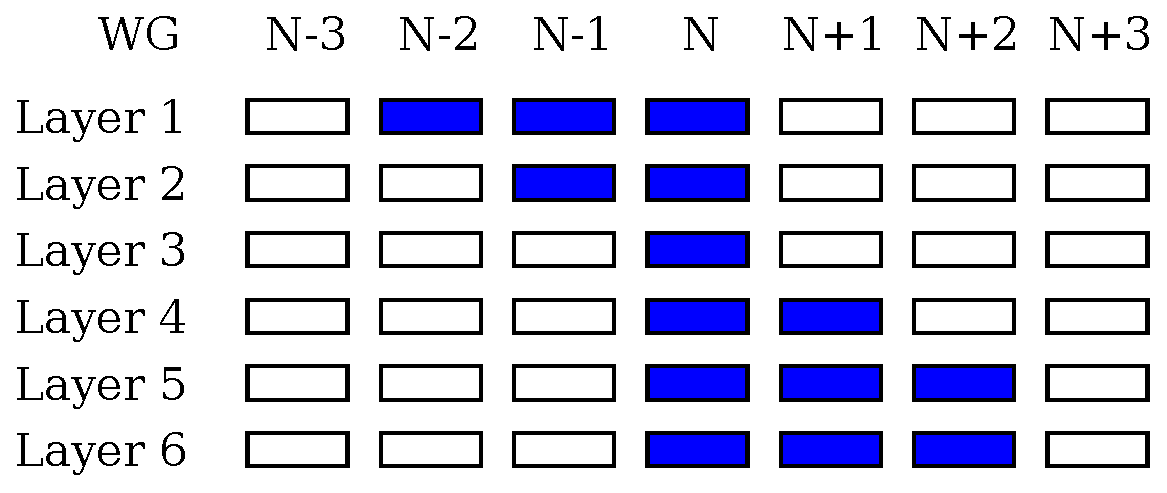
\includegraphics[width=0.49\linewidth]{figures/alct_pretrigger.pdf}\\
                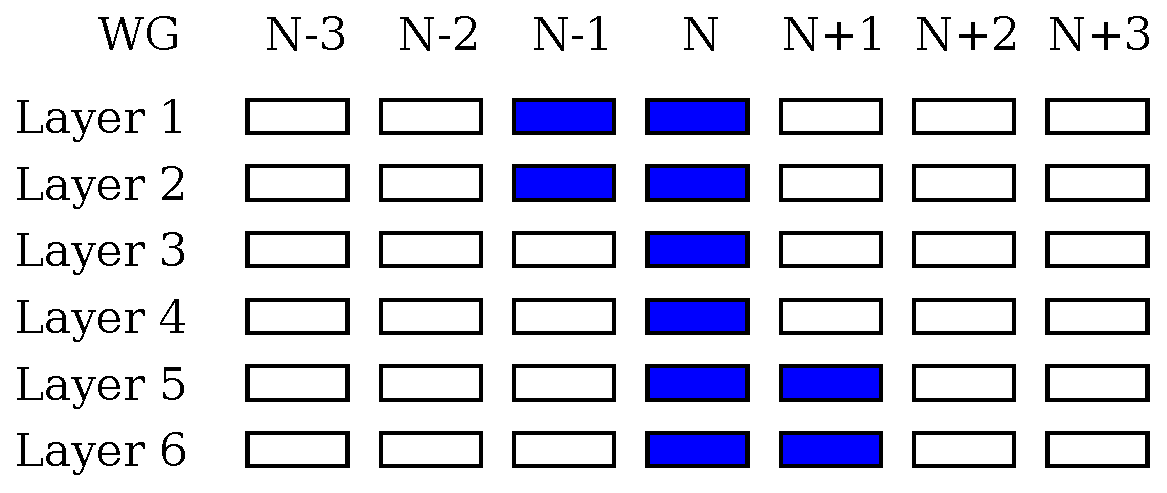
\includegraphics[width=0.49\linewidth]{figures/alct_pretrigger_r1.pdf}
                \caption{Top: default ALCT pattern mask, bottom: narrow ALCT pattern mask.}
                \label{fig:narrow_alct_pattern_mask}
        \end{center}
\end{figure}

The following modifications in configuration are related to this improvement:
\begin{itemize}
    \item alctNarrowMaskForR1: False to True
\end{itemize}

\subsubsection{Reduced ALCT Dead Time}

Currently, if there is pretrigger in BX = B (see Fig.~\ref{fig:alct_deadtime}):
\begin{itemize}
    \item Check for trigger in BX = B + drift time = B+2
    \item Search for next pretrigger starting from BX = B + drift time + extra deadtime = B+6
\end{itemize}

Suggested improvement: decrease extra deadtime from 4 BX to 0 BX.

\begin{figure}[tbh]
        \begin{center}
                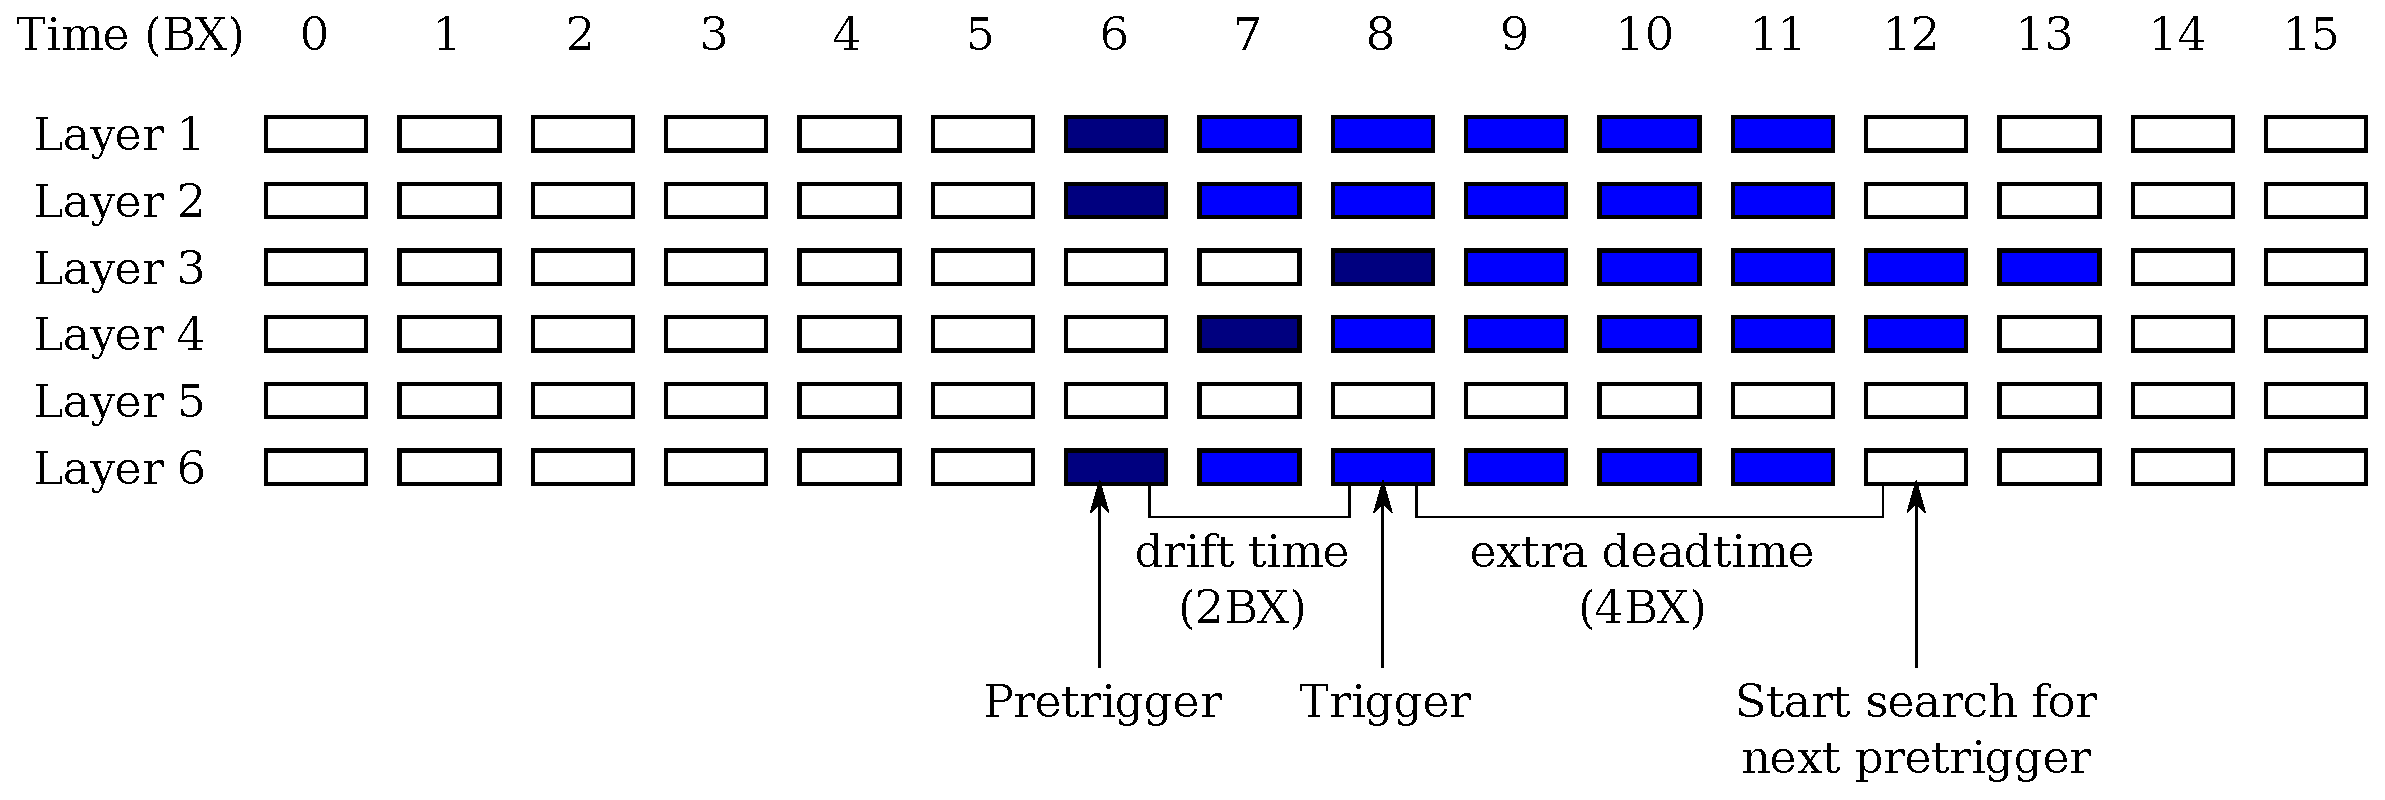
\includegraphics[width=0.98\linewidth]{figures/stretched_hits_alct_deadtime.pdf}
                \caption{Top: Dead Time between ALCT pretriggers.}
                \label{fig:alct_deadtime}
        \end{center}
\end{figure}

The following modifications in configuration are related to this improvement:
\begin{itemize}
    \item alctPretrigDeadtime: 4BX to 0BX
\end{itemize}


\subsection{Results of Improvements of the ALCT Processing}

Improvements on the level of ALCT processor are related to the following configuration parameters (see Sec.~\ref{sec:ALCT_conf}):
\begin{itemize}
	\item alctGhostCancellationBxDepth: 4BX to 1BX;
	\item alctGhostCancellationSideQuality: False to True;
	\item alctNarrowMaskForR1: False to True;
	\item alctPretrigDeadtime: 4BX to 0BX.
\end{itemize}

Fig.~\ref{fig:ALCT_improvements_ALCT_recoEff} shows reconstruction efficiency of a good ALCT in ME1/1 station versus pseudorapidity of the simulated muon for different L1 configurations. The good ALCT is defined as ALCT:
\begin{itemize}
	\item read out in the window of 3BX around the central BX (BX6);
	\item reconstructed within 2 anode wire groups from the key wire group.
	\item has hits at least on four layers
\end{itemize}

The major improvement in ALCT reconstruction efficiency comes from the changes in ALCT ghost cancellation procedure.

\begin{figure}[p]
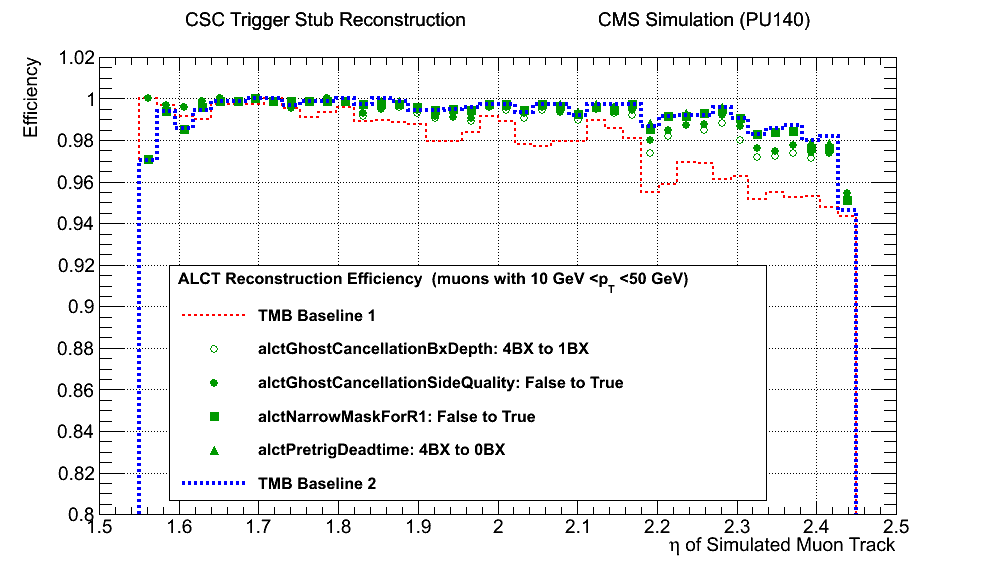
\includegraphics[width=0.98\textwidth]{figures/ALCT_improvements_ALCT_recoEff.png}
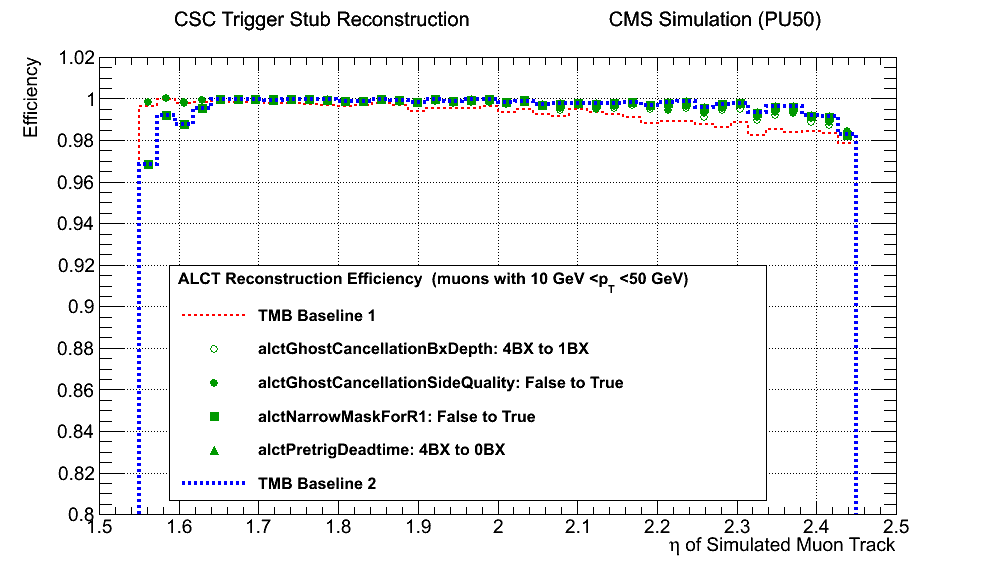
\includegraphics[width=0.98\textwidth]{figures/ALCT_improvements_ALCT_recoEff_PU50.png}
\caption{ALCT reconstruction efficiency in ME1/1 station for PU140 (top) and PU50 (bottom). Muons with transverse momentum $10$~GeV$<p_T<50$~ GeV are used in the analysis.}
\label{fig:ALCT_improvements_ALCT_recoEff}
\end{figure}
\clearpage

\newpage
\tracinginput{sections/sec_algorithm_clct.tex}
%\section{Cathode Signal Processing}
\label{sec:clct}

\subsection{CLCT Algorithm}
\label{subsec:clct_algo}

[We need a good picture illustrating CLCT processing process like in the case of ALCT one]

A muon passing through a CSC chamber will produce distinctive patterns of half-strip
hits in the six-layer endcap muon CSC chambers. By identifying these patterns, the CSC Local
Trigger provides high rejection power against backgrounds. The largest background source,
neutron-induced gamma ray conversions, are generally low in energy, and produce mostly single-
layer or short multi-layer hits. Other backgrounds, such as low-momentum muons or punch-
through particles often do not point well enough to the primary interaction region to be considered
high-momentum muon candidates.

\begin{figure}[tbh]
        \begin{center}
                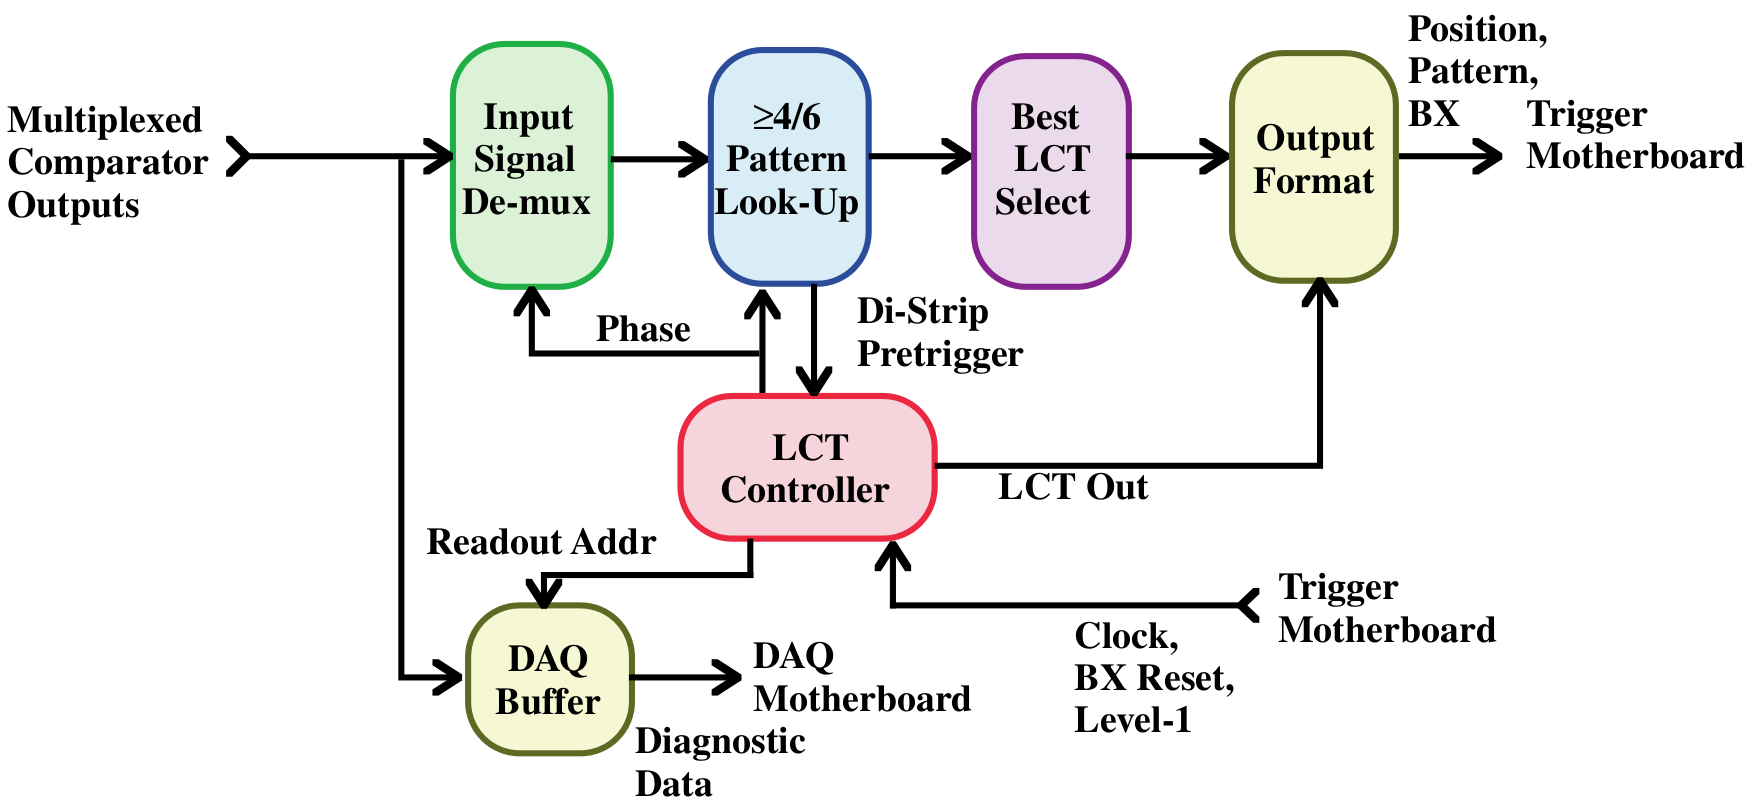
\includegraphics[width=0.73\linewidth]{figures/CLCT_block_diagram.png}
                \caption{CLCT block diagram}
                \label{fig:clct_block_diagram}
        \end{center}
\end{figure}

[Technical description from TMB manual below]

For each of 160 key half-strips consider the 42 neighboring half-strips (i.e. on key 5 use the following half-strips):

\begin{figure}[tbh]
        \begin{center}
                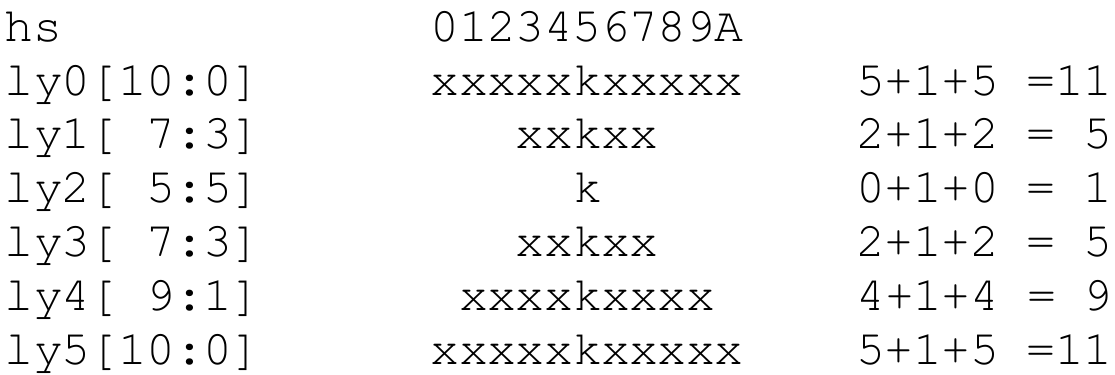
\includegraphics[width=0.48\linewidth]{figures/160_key_half_strips.png}
                \caption{160 key half-strips}
                \label{fig:160_key_half_strips}
        \end{center}
\end{figure}

For each of 160 key half-strips, count layers with hits matching the 9 pattern templates:

\begin{figure}[tbh]
        \begin{center}
                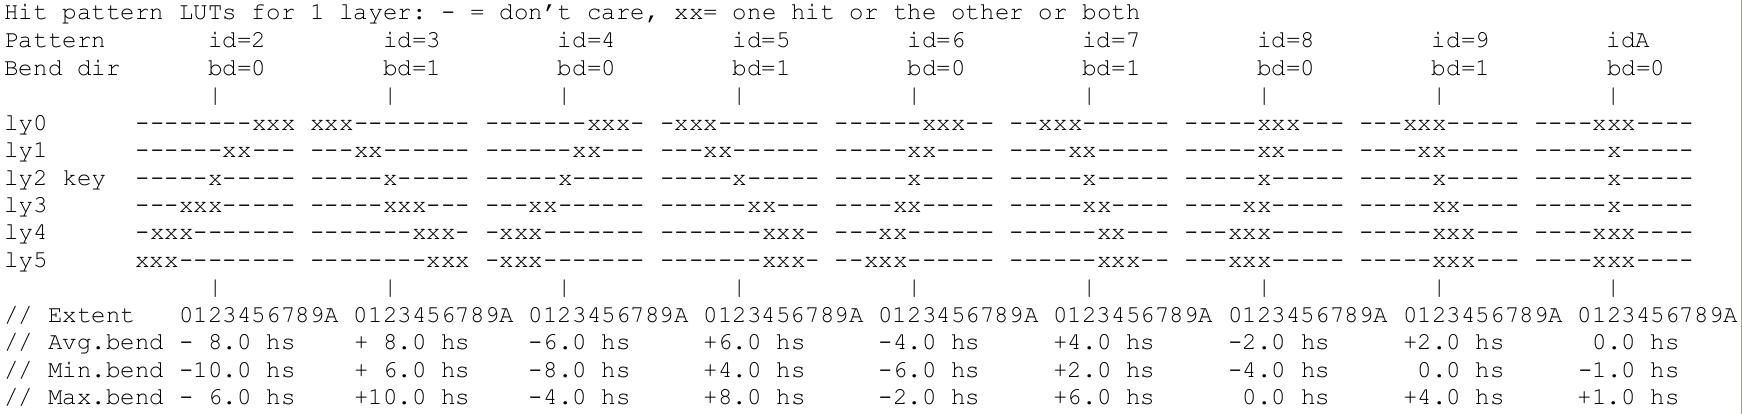
\includegraphics[width=0.98\linewidth]{figures/CLCT_patterns.png}
                \caption{CLCT patterns}
                \label{fig:clct_patterns}
        \end{center}
\end{figure}

Pattern ID=1 is a layer-OR trigger, Pattern ID=0 is no-pattern-found. Result for each of 160 keys is a list of 9 pattern-ID numbers (pid) [2 to A] and corresponding
number of layers [0 to 6] with matching hits (nhits). Find the best 1-of-9 pattern ID numbers for each key by comparing nhits. Ignore bend direction: left and right bends have equal priority (bit 0 of pid implies bend direction).
If two pattern IDs have the same nhits, take the higher pattern ID. A key with no matching hits, would always return pid=A and nhits=0.
Pre-trigger if any 1-of-160 keys have nhits $\geq$ hit\_thresh\_pretrig and pid $\geq$ pid\_thresh\_pretrig.

Construct 7-bit pattern quality pat[7:0] for sorting where pat[7:5]=nhits[2:0], pat[4:0]=pid[3:0]. Ignore the bend direction bit (pid[0]), left and right bends have equal priority. 
Store pat[7:0] for 160 keys for use later to find 2nd CLCT.
Find the best key out 1-of-160 keys by sorting on the 6-bit number pat[7:1]. Store 1st CLCT info: key, pattern ID, and number of hits.
For empty events, key=0, pid=A and nhits=0. If clct\_blanking=1, then key=pid=hits=0.

Mark keys near 1st CLCT as busy from 1st key-nspan to 1st key+pspan.
If clct\_sep\_src=1, pspan and nspan are set equal to clct\_sep\_vme, typically 10 half-strips.
If clct\_sep\_src=0, pspan and nspan are read from RAM and depend on the pattern ID number, this allows two less bending tracks to be closer than more bending tracks.

Find the best key out of 1-of-160 keys by sorting on the 6-bit number pat[7:1]: skip busy keys, if two keys have the same pat[7:1] take the lower key.
Store the same information for the 2nd CLCT as for the 1st one.

Wait for CSC drifting (drift delay of 2BXs) and perform matching to ALCTs.


\subsection{Separation of the CLCTs in ME1/1a and ME1/1b}

In the old TMB f/w, the 16 ganged strip channels from ME1/1a are appended to the 64 ME1/1b strip channels and the reconstruction of CLCTs is performed as if it's a single regular chamber with 80 channels (is there any treatment of the boundary, so that ME1/1a strips are not combined with ME1/1b strips?). The two rather separate and distinctive areas combined and treated like one uniform unit with the maximum of two CLCT stubs on the output.

With unganged ME1/1a and higher pile-up such a simple approach becomes increasingly unnatural and ineffective. The ME1/1a would have x3 more channels now, so it would deserve to be treated like a separate chamber even more. And chances to get multiple stubs are increasing with higher luminosity, especially so in ME1/1a. With multiple stubs, the stubs in ME1/1a would start directly competing with those in ME1/1b.

With a larger size FPGA, it would be beneficial to treat ME1/1a and ME1/1b as two separate chambers for the purpose of CLCT reconstruction, with each area having their own limit on the maximum of 2 CLCTs. Thus, the whole ME1/1 would be able to have maximum 4 CLCTs available for matching with ALCTs. It's important to keep more 2D stubs available so that at the stage of matching we can reduce the number of stubs following some better tuned criteria.

Finally, in the case if we would allow to read out the 2D CLCT stubs without an ALCT match, and we cannot read out more then 2 of them per BX per ME1/1, we can device a selection criteria when comparing stubs from ME1/1a and ME1/1b as follows: e.g., if quality of an ME1/1b stub is the same or less by one then that of an ME1/1a stub, prefer the ME1/1b one. 

\subsection{Localization of the TMB Dead Time}

 The main source of the old TMB inefficiency in high pile-up is the dead time which happens for the whole ME1/1 chamber after there was a triggering CLCT. The TMB's state-machine freezes whole TMB for several BXs after a CLCT trigger while number of coincidence layers stays over the trigger threshold. If anywhere in a chamber there was an CLCT from PU a few BX earlier before a signal muon, it would be impossible to trigger on the signal.

While it's clear that with the comparator information which we recieve in TMB, it's not really possible to distinguish close in time signals in the same strip, there seem to be no apparent reason, other then the complexity of the algorithm, for this dead time to be present in strips that had no trigger.

Thus, the algorithm approach to deal with this issue for the upgrade could be as follows:
\begin{itemize}
    \item when a CLCT trigger happens, mark as busy only those strips within either a fixed dead time zone around CLCT (8 half-strips, see "useDeadTimeZoning" parameter in Sec.~\ref{sec:CLCT_conf}) or within the dead time zone, the width of which depends on the CLCT pattern (from 11 half-strips for the most bent patterns to 3 half-strips for the straightest one, see "useDynamicStateMachineZone" parameter in Sec.~\ref{sec:CLCT_conf}), and also mark the signal half-strip that specifies the triggered CLCT
    \item during the following bunch-crossings, check if the number of coincidence layers drops under the trigger threshold for the signal half-strip
    \begin{itemize}
	\item if it does, remove the "busy" mark from the corresponding strips 
    \end{itemize}
    \item if strips are marked as busy in a BX, they are excluded from pattern recognition 
\end{itemize}

\subsection{Restriction on the CLCT Pattern Bend}

The current set of CLCT patterns (see details in Sec.~\cite{subsec:clct_algo}) is largely geared towards low pt tracks. For tracks with pt>10, only the straighest and the next one bent patterns are significant. The restriction on allowed pattern bending would significantly help with many issues including multiplicity \& rate, ghosting, dead-time and corresponding loss of the efficiency (see "clctPidThreshPretrig" parameter in Sec.~\ref{sec:CLCT_conf}). Positive effect of it would increase with increasing luminosity. However, it would also somewhat reduce the efficiency because of not so good pt-threshold resolution from fairly narrow (11cm) CSC chambers, especially for medium to lower pt muons.

Plots on Fig.~\ref{fig:efficiency_vs_pt} show the efficiency vs $p_T$ for a simulated muon track to have a matching reconstructed CLCT stub for different sets of patterns (which defines maximum thresholds for the bend). Note, that adding GEMs could be helpful for improving the the efficiency of the bend restriction.

\begin{figure}[tbh]
        \begin{center}
                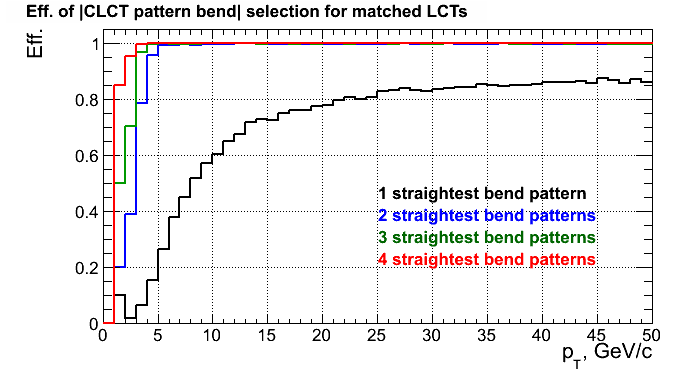
\includegraphics[width=0.48\linewidth]{figures/efficiency_vs_pt.png}
                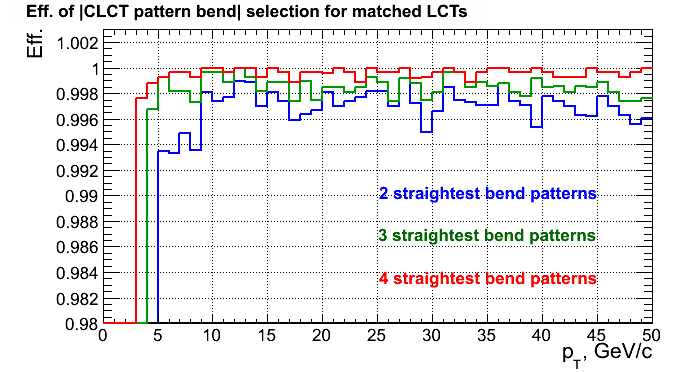
\includegraphics[width=0.48\linewidth]{figures/efficiency_vs_pt_scale.png}
                \caption{Efficiency vs $p_T$. No pile up is included in the simulated sample.}
                \label{fig:efficiency_vs_pt}
        \end{center}
\end{figure}

\subsection{Improvement of the CLCT Timing}

Currently, the BX time of a CLCT stub is defined as the BX of its pretrigger. Or, in other words, it's first BX when at least three layers fit one of the CLCT patterns. Note that an attempt to latch a trigger pattern is performed after the number of BX after the pretrigger defined by the clctDriftDelay parameter (=2BX). And also note that a CLCT pattern during the pretrigger could be different then the one that happen to match during the trigger.

With higher luminosity there are increasingly larger chances for some strips in some of the layers to be hit by earlier background hit. And that has chances to affect the time when a pretrigger might be detected. A more robust solution would be to define stub's time using the times of its strips, where stub's strips are defined as strips that were matched within a CLCT pattern during the trigger. As for a specific procedure, a median time over those strips' times or some sort of a truncated average could be used (see "clctUseCorrectedBx" parameter in Sec.~\ref{sec:CLCT_conf}, analogously for "alctUseCorrectedBx" parameter in Sec.~\ref{sec:ALCT_conf}).

\newpage
\subsection{Software Emulation of CLCT Processing}

CLCT processing includes the following four steps:

\begin{itemize}
    \item Pulse extension;
    \item Pretrigger;
    \item Trigger;
    \item CLCT construction and CLCT dead time.
\end{itemize}

In contrast to ALCT processing, where all steps are independent and performed one after another for all 16 BXs, during CLCT processing last three steps repeated in one global loop over BXs.

\subsubsection{Pulse Extension}

Sofware emulation provides information about all half-strip signals in DAQ readout window (16 BXs). A search for these signals is performed in a loop over all half-strips, all layers, and all 16 BXs; found signals are stretched over 6 BXs (see Fig.~\ref{fig:clct_pulse_extension}).

\begin{figure}[tbh]
        \begin{center}
                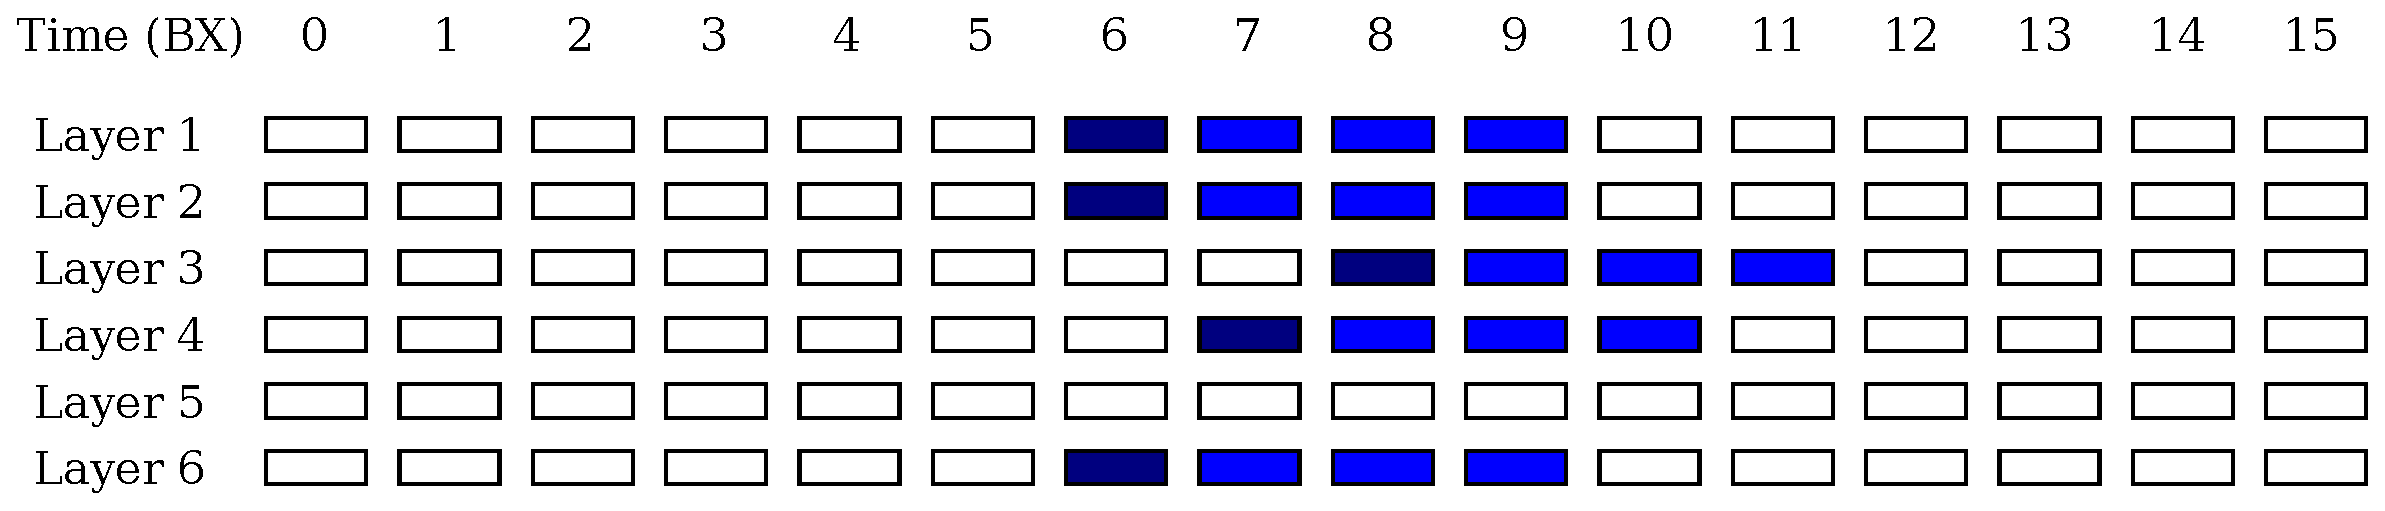
\includegraphics[width=0.9\linewidth]{figures/stretched_hits_clct.pdf}
                \caption{Illustration of ALCT pulse extension for one specific half-strip.}
                \label{fig:clct_pulse_extension}
        \end{center}
\end{figure}

\subsubsection{Pretrigger}

After all available half-strip signals are stretched, start a global loop over all BXs from BX = 0 and search for CLCT pretriggers in all half-strips. For any given BX and half-strip, count the number of layers with hits within the patterns shown on Fig.~\ref{fig:clct_pretrigger}, and if this number is greater than or equal to three, then we say that a pretrigger occured in this BX and this half-strip. This pretrigger is only accepted if its pattern id $\geq$ 2. If there were no CLCTs found in some BX = B, proceed to BX = B+1 and continue searching for pretriggers. If there are some CLCTs found in the current BX, proceed to next step.

\begin{figure}[tbh]
        \begin{center}
                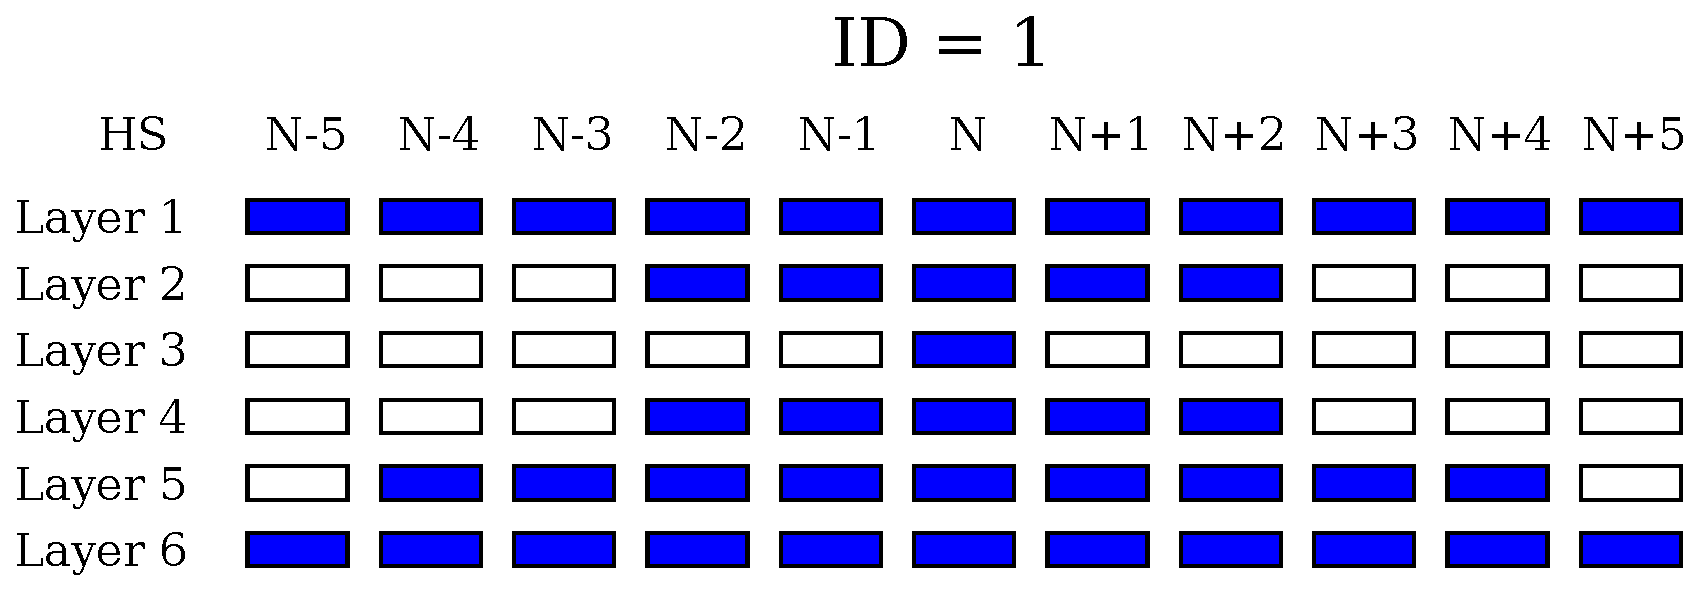
\includegraphics[width=0.48\linewidth]{figures/clct_pattern_01.pdf}
                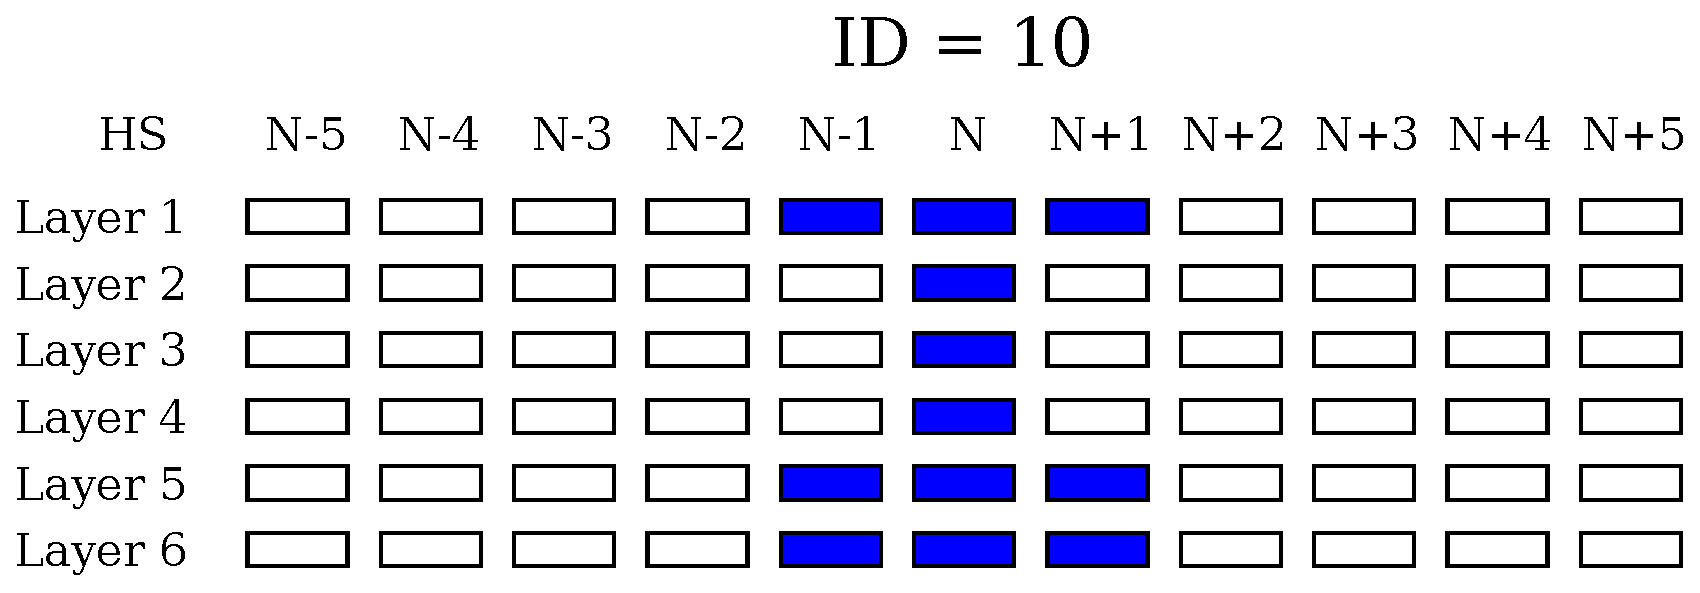
\includegraphics[width=0.48\linewidth]{figures/clct_pattern_10.pdf}\\
                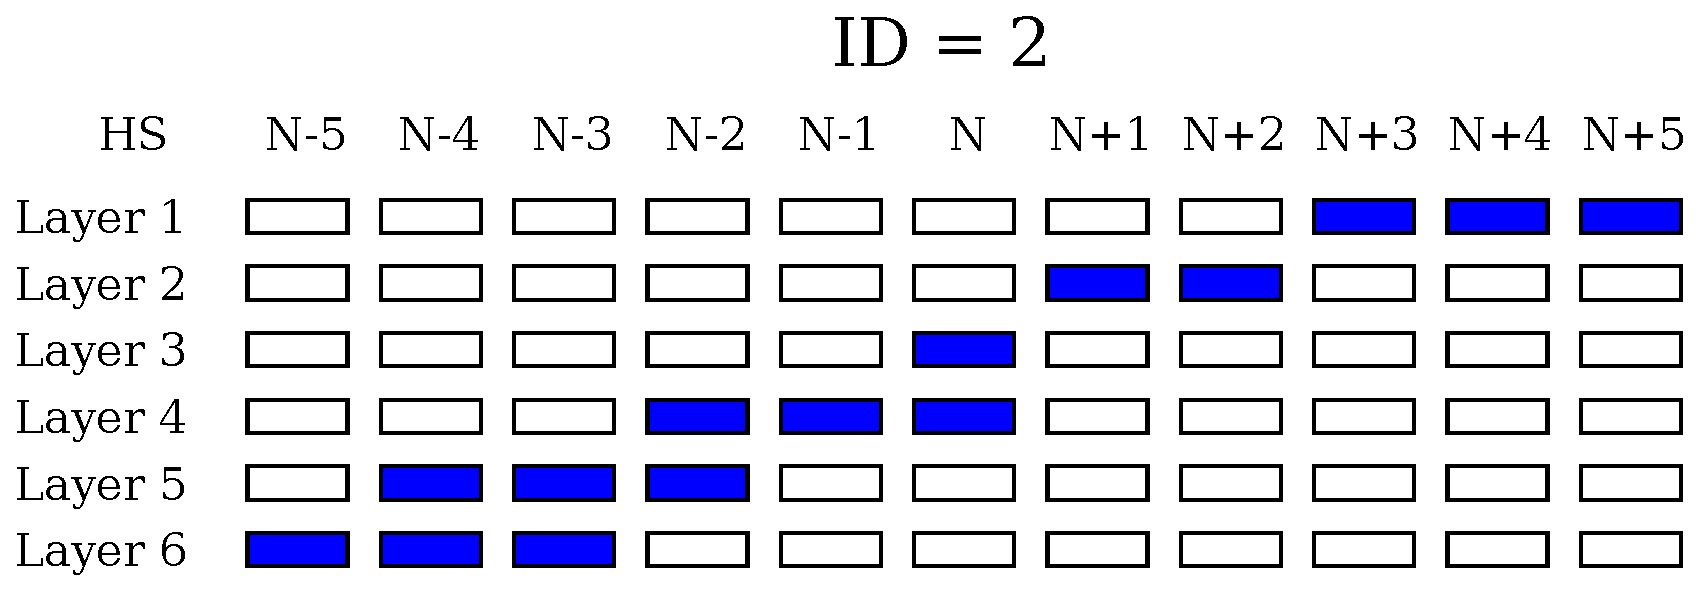
\includegraphics[width=0.48\linewidth]{figures/clct_pattern_02.pdf}
                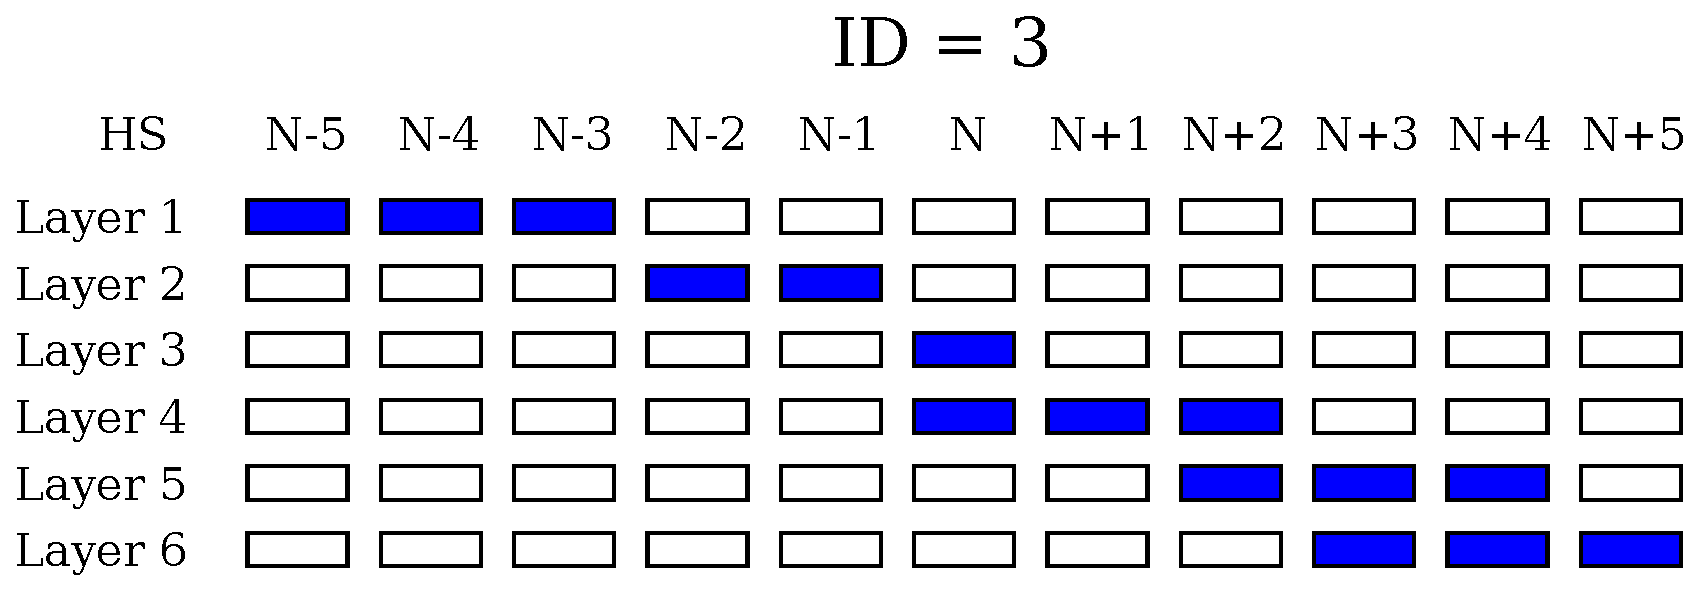
\includegraphics[width=0.48\linewidth]{figures/clct_pattern_03.pdf}\\
                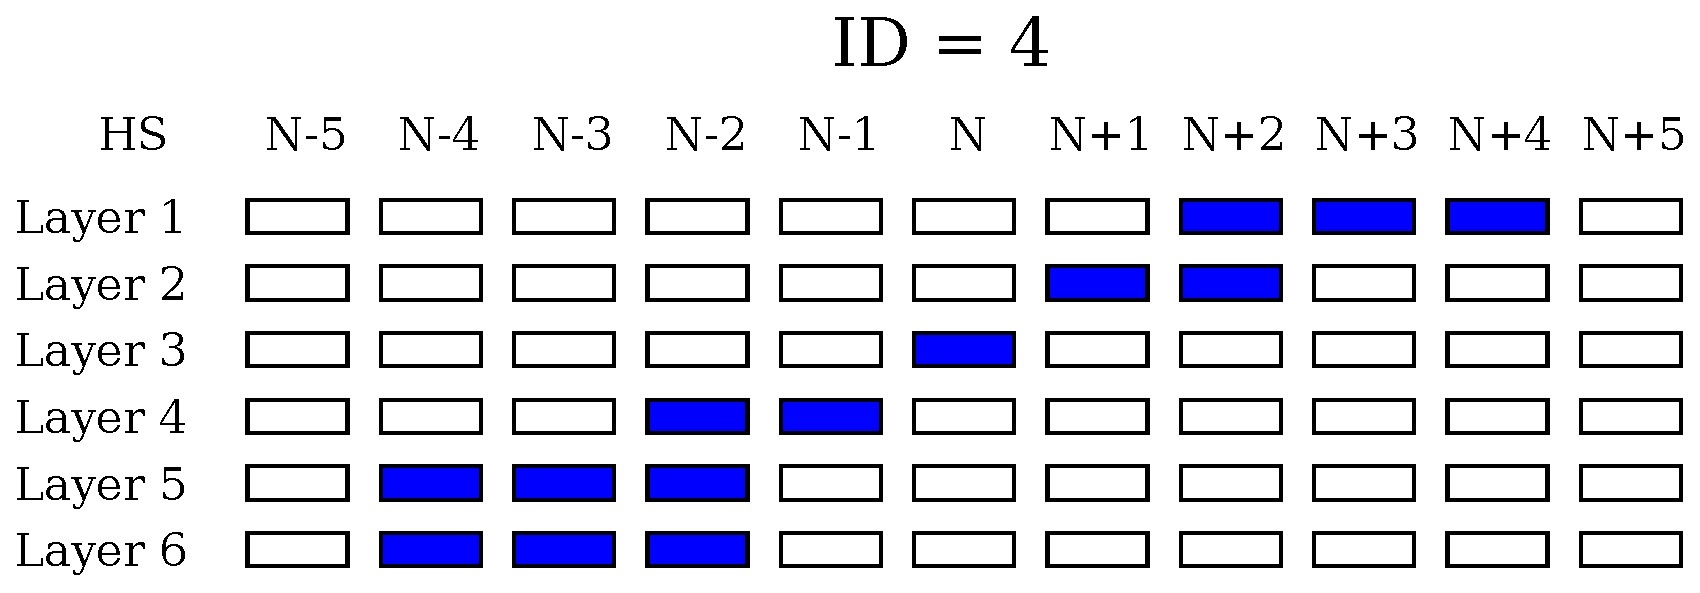
\includegraphics[width=0.48\linewidth]{figures/clct_pattern_04.pdf}
                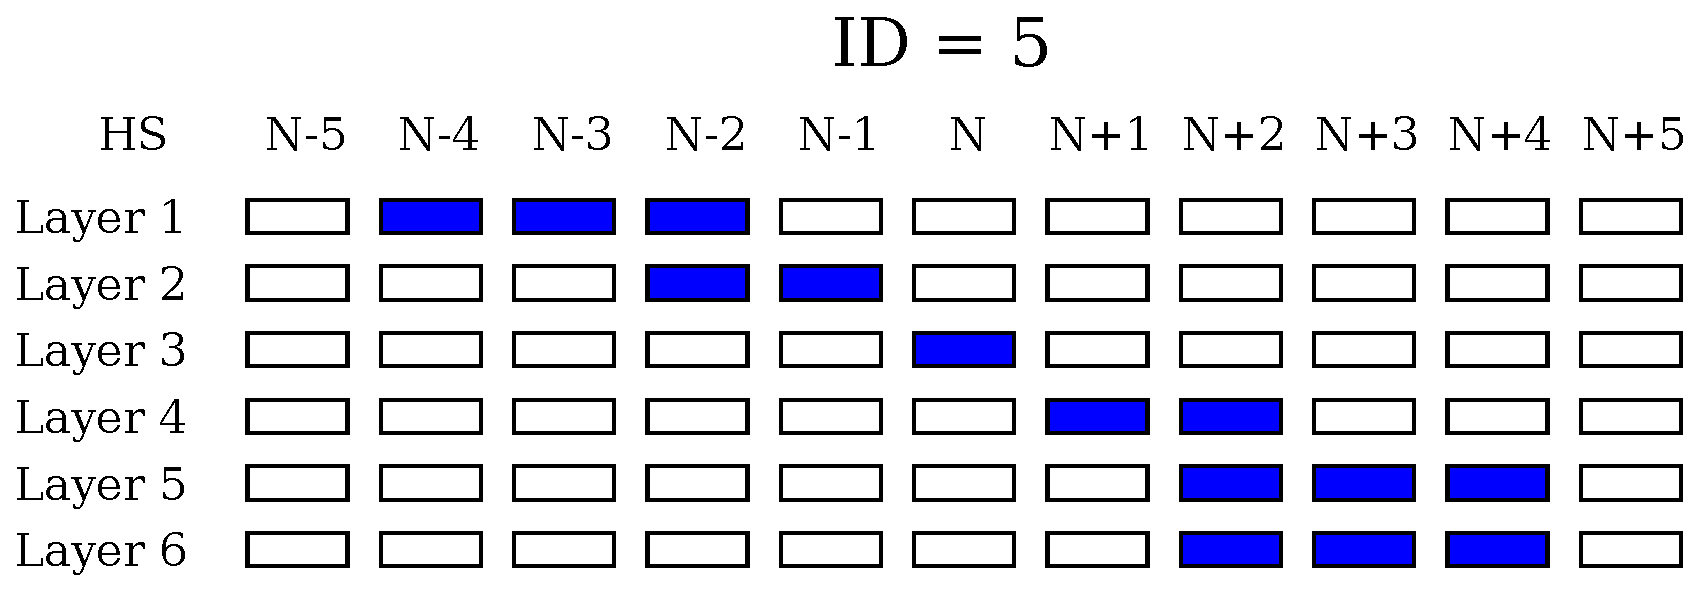
\includegraphics[width=0.48\linewidth]{figures/clct_pattern_05.pdf}\\
                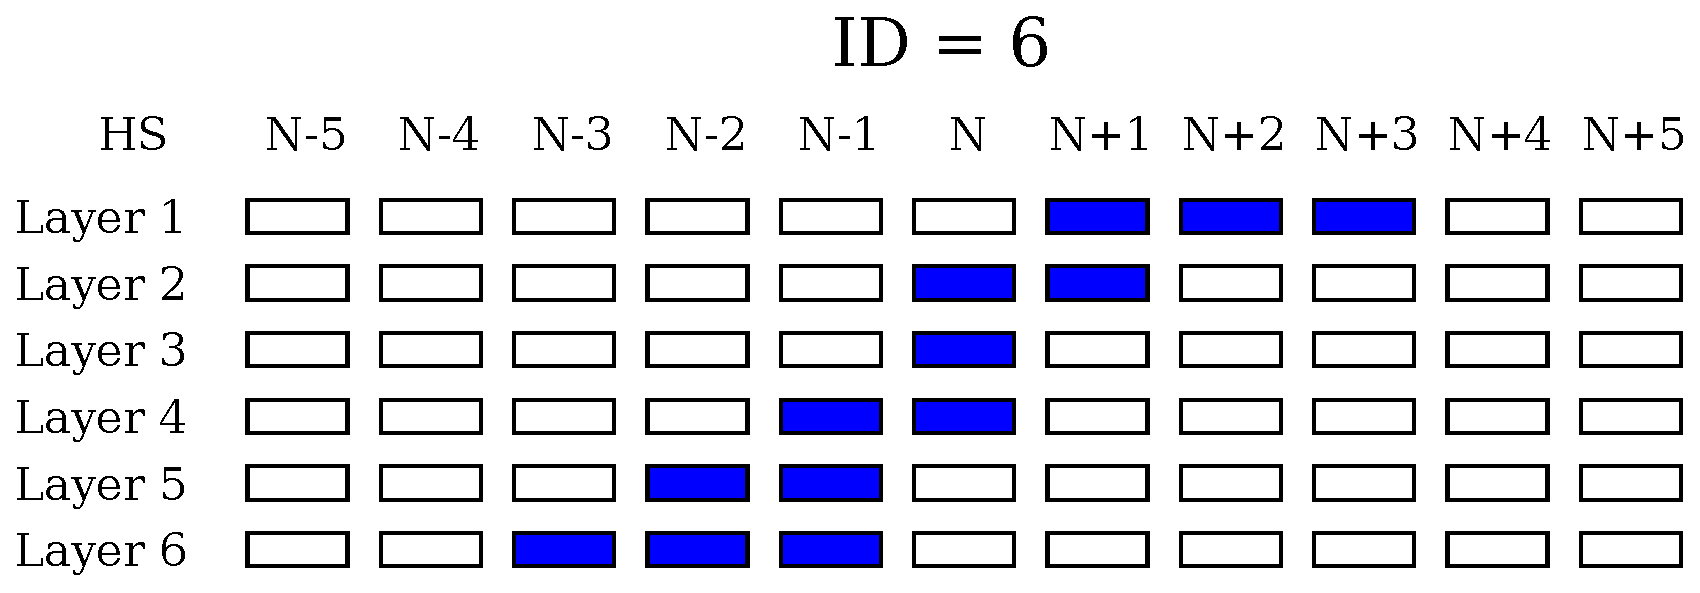
\includegraphics[width=0.48\linewidth]{figures/clct_pattern_06.pdf}
                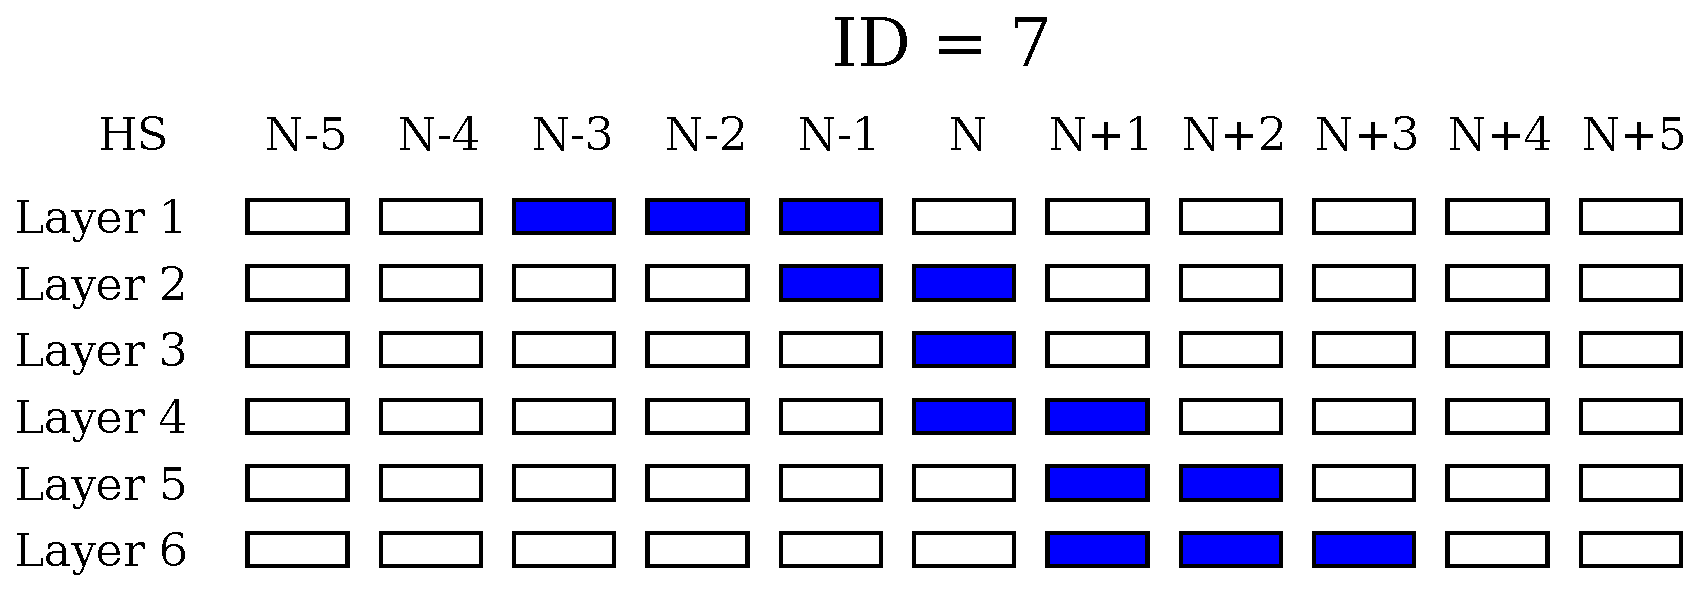
\includegraphics[width=0.48\linewidth]{figures/clct_pattern_07.pdf}\\
                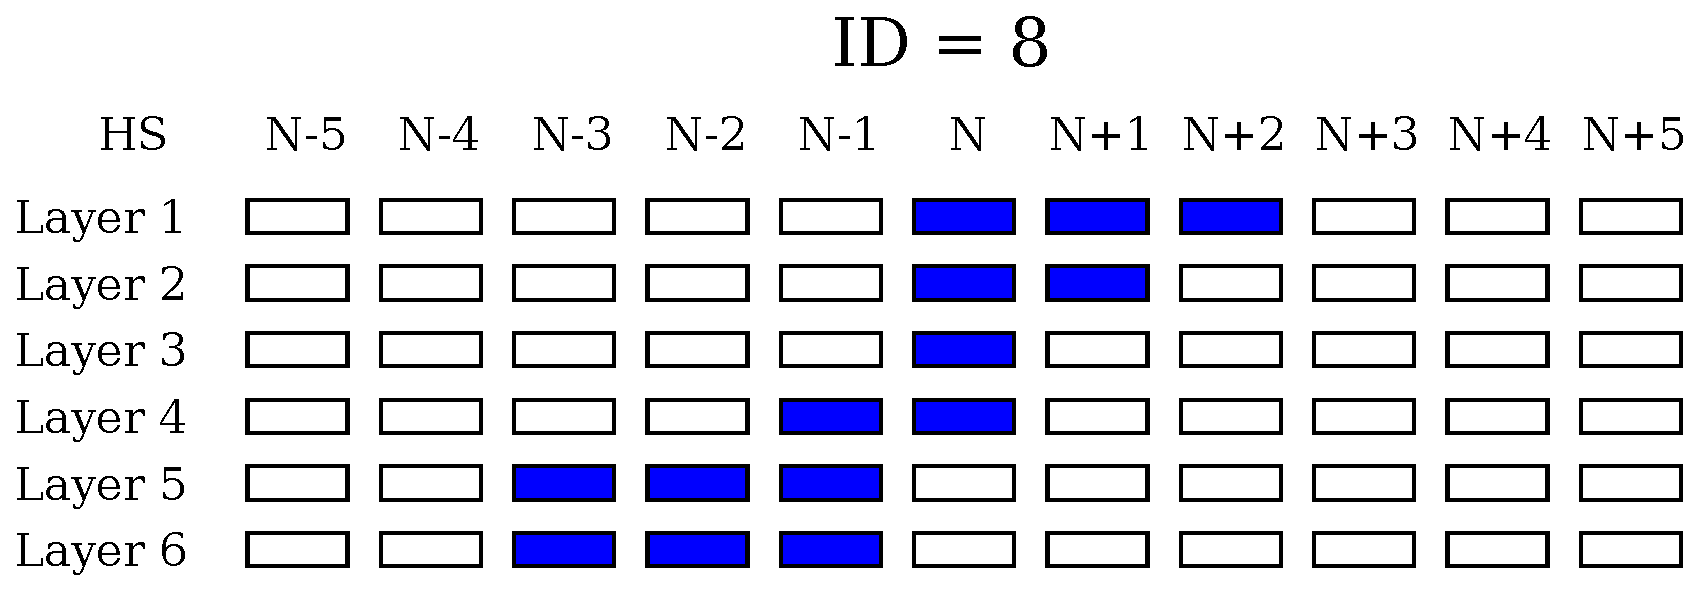
\includegraphics[width=0.48\linewidth]{figures/clct_pattern_08.pdf}
                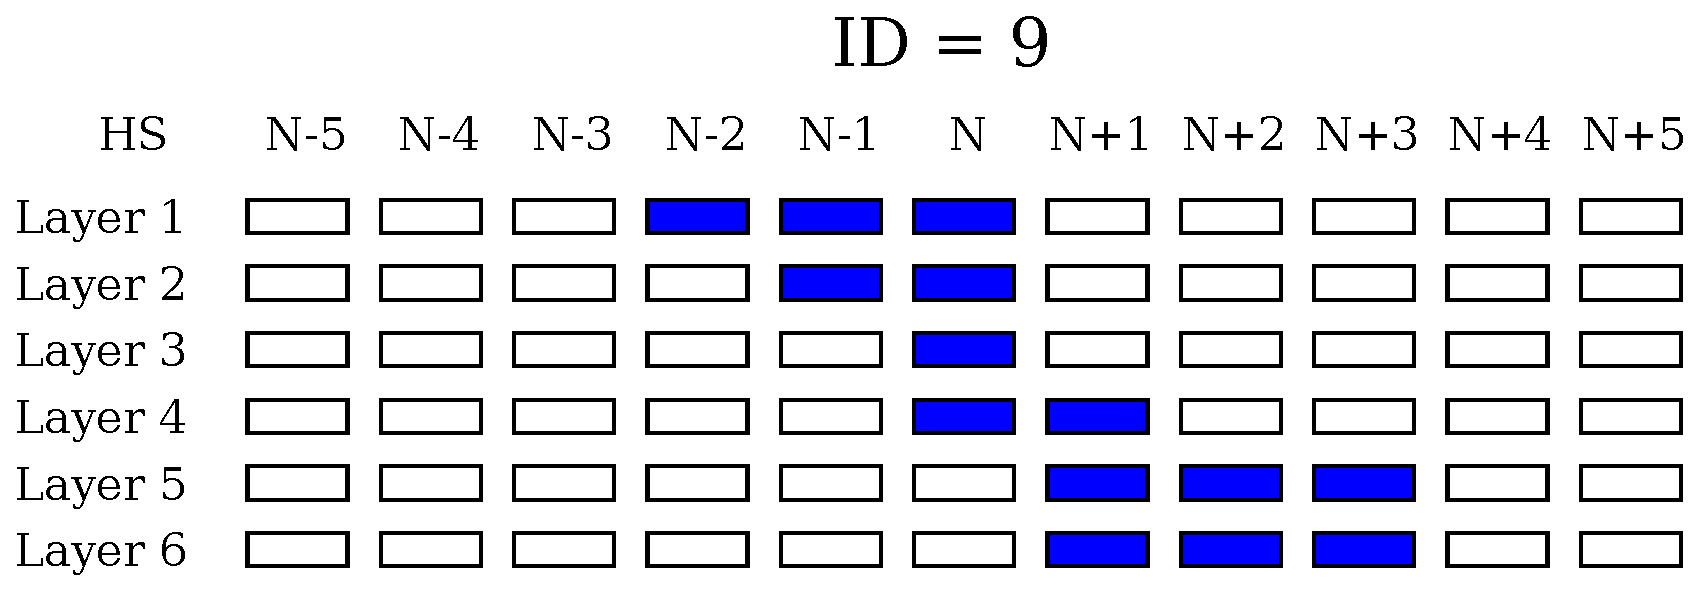
\includegraphics[width=0.48\linewidth]{figures/clct_pattern_09.pdf}
                \caption{CLCT patterns for pretriggering and triggering.}
                \label{fig:clct_pretrigger}
        \end{center}
\end{figure}

\subsubsection{Trigger}

As soon as a BX = B with CLCT pretrigger(s) is found, search for triggers in BX = B+2. For each half-strip, count the number of layers with hits within the same patterns used for pretriggering, and if this number is greater than or equal to four, we say that a trigger occured in this half-strip and BX, and remember:
\begin{itemize}
    \item pattern id with the highest number of hit layers (if there are two pattern ids with the same number of hit layers, choose smaller pattern id);
    \item number of hit layers in this pattern id.
\end{itemize}

Proceed to next step.

\subsubsection{CLCT Construction and CLCT Dead Time}

In a BX with CLCT triggers, find up to two best triggers to be used in CLCT construction.

Find the best trigger:
\begin{itemize}
    \item Find trigger with the highest number of hit layers;
    \item If there are two triggers with the same number of hit layers: choose the one with higher pattern id;
    \item If there are two triggers with the same number of hit layers and the same pattern id: choose the one with smaller half-strip.
\end{itemize}

Mark zone of 20 half-strips around the best trigger as used and find the second best trigger among not used half-strips.

Construct up to two best CLCTs from found best triggers: encode quality, pattern, bending direction, half-strip, cfeb, BX (defined by pretrigger BX).

After CLCT construction, keep CLCT "dead": continue the loop over all BXs until there is a BX with no triggers. When such a BX is found go back to pretriggering step.


\newpage
\subsection{Sofware Emulation of CLCT Level Improvements}

\subsubsection{Localizing Dead Zone}

\textcolor{red}{Current implementation of dead time}:
\begin{itemize}
    \item After constructing up to two CLCTs, \textcolor{red}{continue the loop over all BXs until there is a BX with no triggers}
    \\...
    \item In the BX with trigger, construct up to two CLCTs from two best triggers \textcolor{red}{in all half-strips}
    
\end{itemize}
\textcolor{blue}{New implementation of dead time}:
\begin{itemize}
    \item After constructing up to two CLCTs, \textcolor{blue}{mark 16 half-strips around half-strips of these CLCTs as busy while number of hit layers in half-strips of these CLCTs $\geq$ 4}
    \item \textcolor{blue}{After trigger in BX = B, keep searching for pretrigger in strating from BX = B+1}
    \\...
    \item In the BX with trigger, construct up to two CLCTs from two best triggers \textcolor{blue}{in half-strips}
    \begin{itemize}
        \item \textcolor{blue}{within 5 half-strips from pretrigger half-strips}
        \item \textcolor{blue}{which are not marked as busy from previous trigger}
    \end{itemize}
\end{itemize}

The following modifications in configuration are related to this improvement:
\begin{itemize}
    \item useDeadTimeZoning: False to True
\end{itemize}

\subsubsection{Dynamic Dead Zone Width}

\textcolor{red}{Fixed dead time zone}:
\begin{itemize}
    \item After constructing up to two CLCTs, mark \textcolor{red}{16} half-strips around half-strips of these CLCTs as busy while number of hit layers in half-strips of these CLCTs $\geq$ 4
\end{itemize}
\textcolor{blue}{Dynamic dead time zone}:
\begin{itemize}
    \item After constructing up to two CLCTs, mark \textcolor{blue}{K(pid)} half-strips around half-strips of these CLCTs as busy while number of hit layers in half-strips of these CLCTs $\geq$ 4
\end{itemize}
\vskip3mm
K(pid) --- function of pattern id:
\begin{itemize}
    \item K(1,2,3) = 22 half-strips
    \item K(4,5) = 18 half-strips
    \item K(6,7) = 14 half-strips
    \item K(8,9) = 10 half-strips
    \item K(10) = 6 halt-strips
\end{itemize}

The following modifications in configuration are related to this improvement:
\begin{itemize}
    \item useDynamicStateMachineZone: False to True
\end{itemize}

\newpage

\subsubsection{Minimal Pattern ID for Pretriggering}

\textcolor{red}{Current CLCT pretrigger}:
\begin{itemize}
    \item Loop over all BXs (starting from BX = 0) and all half-strips:
    \begin{itemize}
        \item Count number of layers with hits in the following patterns
        \item If this number $\geq$ 3: pretrigger occurs
        \item Accept this pretrigger if its pattern id $\geq$ \textcolor{red}{2}
    \end{itemize}
\end{itemize}
\textcolor{blue}{New CLCT pretrigger}:
\begin{itemize}
    \item Loop over all BXs (starting from BX = 0) and all half-strips:
    \begin{itemize}
        \item Count number of layers with hits in the following patterns
        \item If this number $\geq$ 3: pretrigger occurs
        \item Accept this pretrigger if its pattern id $\geq$ \textcolor{blue}{4}
    \end{itemize}
\end{itemize}

The following modifications in configuration are related to this improvement:
\begin{itemize}
    \item clctPidThreshPretrig: 2 to 4
\end{itemize}

\subsubsection{Minimal Separation Between Two Best CLCTs}

\textcolor{red}{Current construction of up to two CLCTs}:
\begin{itemize}
    \item Search for the best trigger in this BX
    \item Mark \textcolor{red}{20} half-strips around the best trigger as busy
    \item Find the second best trigger among non-busy half-strips
\end{itemize}
\textcolor{blue}{New construction of up to two CLCTs}:
\begin{itemize}
    \item Search for the best trigger in this BX
    \item Mark \textcolor{blue}{10} half-strips around the best trigger as busy
    \item Find the second best trigger among non-busy half-strips
\end{itemize}

The following modifications in configuration are related to this improvement:
\begin{itemize}
    \item clctMinSeparation: 10 to 5 cathode strips
\end{itemize}


\subsection{Results of Improvements of the CLCT Processing}

Improvements on the level of CLCT processor are related to the following configuration parameters (see Sec.~\ref{sec:CLCT_conf}):
\begin{itemize}
	\item useDeadTimeZoning: False to True;
	\item useDynamicStateMachineZone: False to True;
	\item clctPidThreshPretrig: 2 to 4;
	\item clctMinSeparation: 10 to 5 cathode strips.
\end{itemize}

Fig.~\ref{fig:CLCT_improvements_CLCT_recoEff} shows reconstruction efficiency of a good CLCT in ME1/1 station versus pseudorapidity of the simulated muon for different L1 configurations. The good CLCT is defined as CLCT:
\begin{itemize}
        \item read out in the window of 3BX around the central BX (BX6);
        \item reconstructed within 2 cathode strips from the key strip.
	\item has hits at least on four layers
\end{itemize}

The major improvement in CLCT reconstruction efficiency comes from localization of the deadtime zone.

\begin{figure}[p]
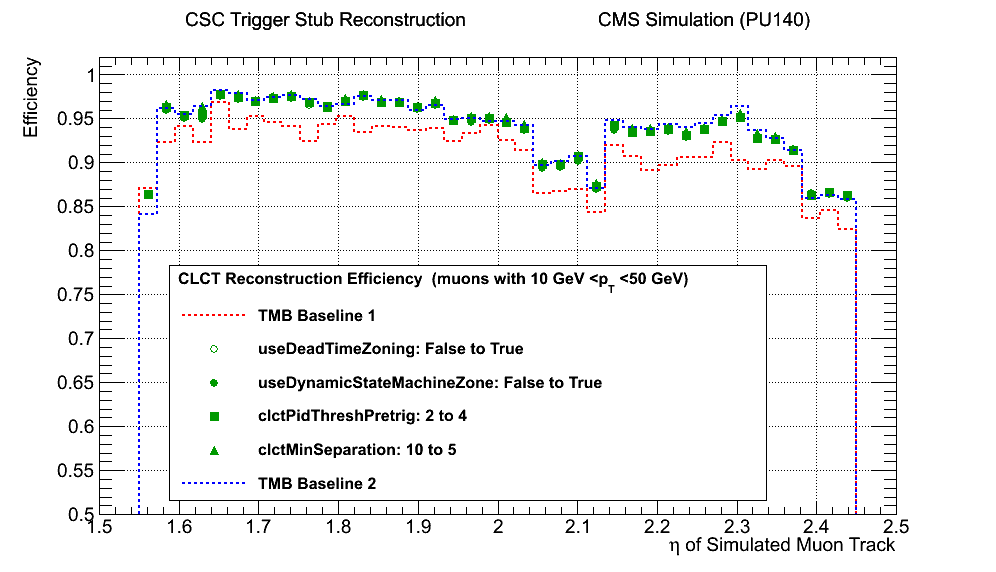
\includegraphics[width=0.98\textwidth]{figures/CLCT_improvements_CLCT_recoEff.png}
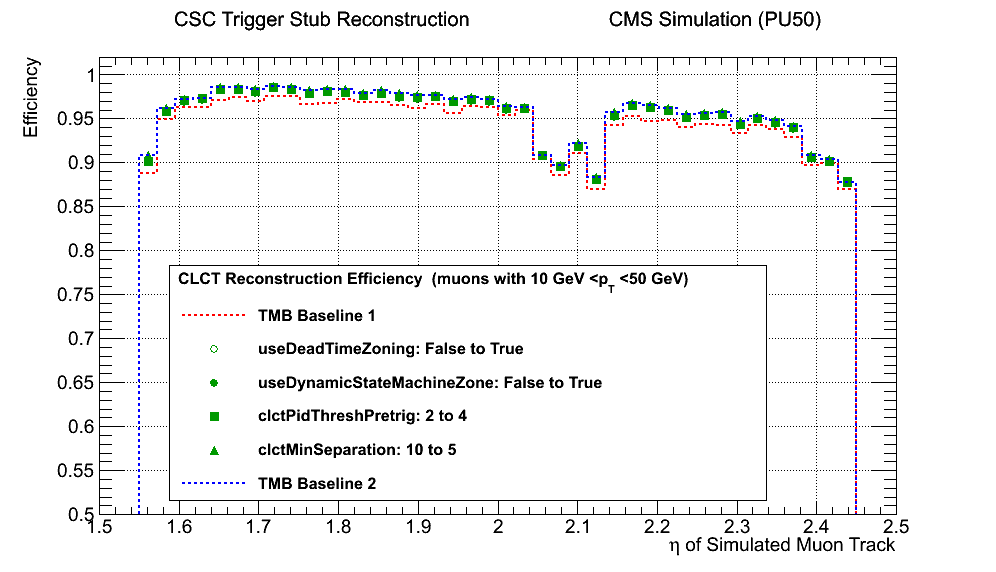
\includegraphics[width=0.98\textwidth]{figures/CLCT_improvements_CLCT_recoEff_PU50.png}
\caption{CLCT reconstruction efficiency in ME1/1 station for PU140 (top) and PU50 (bottom). Muons with transverse momentum $10$~GeV$<p_T<50$~ GeV are used in the analysis.}
\label{fig:CLCT_improvements_CLCT_recoEff}
\end{figure}
\clearpage

\newpage
\tracinginput{sections/sec_algorithm_lct.tex}
%\section{Cathode-Anode Correlation}

\label{sec:lct}

\subsection{LCT Algorithm}
\label{subsec:lct_algo}

The Trigger Motherboard (TMB) portion of the CLCT/TMB card receives up to two
anode stubs from the ALCT board and two cathode stubs from the CLCT portion of the CLCT/
TMB card. The functions of the TMB circuitry are:

\begin{itemize}
	\item Bunch crossing alignment of the anode and cathode tags.
	\item Correlation of the Anode and Cathode LCT words and construction of two combined LCTs.
	\item Transmission of LCT data to the Muon Port Card (MPC) for triggering, and transmission of DAQ data to the DAQ Motherboard (DAQMB).
\end{itemize}

Incoming anode and cathode LCTs are not aligned in time. Anode LCTs are created
faster than cathode LCTs because of the slow development of the cathode preamp signal, and
because processing inside the ALCT card is faster than processing inside the CLCT logic. The
TMB contains input pipeline logic in order to delay anode LCTs for a programmable number of
bunch crossings up to 10.

The anode and cathode LCTs are matched according to the more precise ALCT bunch
crossing number (BXN). The Cathode LCT BXN can differ by at most $\pm$1 bunch crossing. For each
of the selected muons the TMB outputs a 2-bit bunch crossing match word as shown in
table below. These may be used by later boards in the trigger chain if additional quality information
is needed. They also allow the analysis of the bunch crossing matching in the TMB, since a large
number of bad matches could be an indication of a timing alignment problem.

The ideal case for a high-momentum muon is one anode and one cathode LCT pattern.
However, other cases may occur, which are distinguished by a 2-bit “STA” (Status type A) code:

\begin{itemize}
	\item The TMB may receive one or two anode LCTs and zero cathode LCT patterns. This
happens, for example, for very low-momentum muons. Although the non-zero data is
forwarded to the MPC, this case is flagged by STA=1, as is the similar case of one or two
cathode LCT and zero anode LCT patterns.
	\item If the TMB receives two anode LCTs and one cathode LCT, the TMB outputs two LCTs,
by copying the Cathode LCT bits into both muons. These, and the similar case of two
cathode LCTs and one anode LCT, are flagged by STA=2.
	\item If there are two anode LCTs and two cathode LCTs in one chamber, they are matched
according to their pattern numbers: the largest ALCT and CLCT pattern numbers are
paired, and the second largest ALCT and CLCT pattern numbers are paired. These, and
the ideal case of a single match, are flagged by STA=3.
\end{itemize}

TMBs maintain a local Bunch Crossing Number (BXN) using signals from the Clock
and Control Board. The internal BXN is compared to the BXN received from the ALCT module,
and the Sync Error bit is set if a mismatch is detected.

The TMB sends up to two anode LCT and two cathode LCT patterns for one CSC
chamber to the MPC every 25 ns.

\subsection{Reduction of the Matching Time Window}

The current TMB uses a rather wide time matching window (7BX) that is centered on a CLCT's BX, and is used to look for an ALCT match within it. A wide matching window is not good in high pileup, as propability of incorrect matching with background 2D stubs is higher, resulting in inefficiency.

For the SLHC, we can probably assume that the system is well timed and that we can use the narrowest reasonable matching window of 3BX wide (see "matchTrigWindowSize" parameter in Sec.~\ref{sec:TMB_conf}). 

\subsection{Modification of the Stub Timing Logic in Matching}

 In the old TMB algorithm, the stub timing logic works during the 2D stubs matching as follows:
\begin{itemize}
    \item CLCT-centric approach: CLCTs and their BX are taken as reference points, while ALCTs are waiting in a queue
    \item for a BX with CLCTs we look for a first BX in the matching window that has ALCTs
    \item after matching is dome in this BX, the ALCTs from there are taken off the queue, and cannot be matched with any later CLCT (see "tmbDropUsedClcts" and "matchEarliestClctME11Only" parameters in Sec.~\ref{sec:TMB_conf})
\end{itemize}

The main issues with this approach at high luminosity is that when there is an ALCT from a good signal muon, early CLCTs from background might steal it and form wrong match, and this correct ALCT then would not be available anymore for matching with a later correct CLCT.

Proposal to improve the situation:
\begin{itemize}
    \item ALCT-centric approach: ALCTs and their BXs are taken as reference points, while reconstructed CLCTs are waiting in a matching window-wide queue (see "clctToAlct" parameter in Sec.~\ref{sec:TMB_conf})
    \begin{itemize}
        \item ALCT's BX and the middle BX in the matching window-wide queue are expected to be synchronized 
    \end{itemize}
    \item for an ALCT's BX we look for CLCTs within the queue in the order of arrival try to find maximum 2 LCT matches as follows (see "tmbCrossBxAlgorithm" parameter in Sec.~\ref{sec:TMB_conf}):
    \begin{itemize}
        \item first look for CLCTs in the same BX 2) if we didn't get 2 LCT matches yet, look for CLCTs in BX-1
        \item if we didn't get 2 LCT matches yet, look for CLCTs in BX+1
        \item etc... depending on how wide the matching window is 
    \end{itemize}
    \item can optionally either remove CLCTs from the queue after there was an LCT match, or can keep them for reuse possibilities to be matched with later ALCTs (see "tmbDropUsedClcts" parameter in Sec.~\ref{sec:TMB_conf})
    \item NOTE: all this is supposed to be done separately in ME1/1a and in ME1/1b 
\end{itemize}

\subsection{Selection of the Two Best LCTs per ME1/1}

With the backplane limitations, we can read out only up to two trigger stubs per BX from the whole ME1/1.

Since ME1/1a and ME1/1b now can each have up to two stubs, we need an extra step of selecting the best two ME1/1 stubs out of possible 4. If ME1/1a + ME1/1b has more then two LCTs:
\begin{itemize}
    \item The simplest solution:
    \begin{itemize}
	\item drop the highest eta ones until we have just two. 
    \end{itemize}
    \item Possible improvement:
    \begin{itemize}
        \item rank stubs by special quality value which is the same as stub quality for ME1/1b and is stub quality-1 for ME1/1a stubs
        \item if special quality is the same, rank by eta 
    \end{itemize}
\end{itemize}

\newpage
\subsection{Software Emulation of CLCT and ALCT Matching}

Every BX OTMB receives up to 2 CLCTs and up to two ALCTs from CLCT and ALCT processors, Fig.~\ref{fig:clcts_alcts} shows an example which will be used throughout the subsection.

\begin{figure}[tbh]
        \begin{center}
                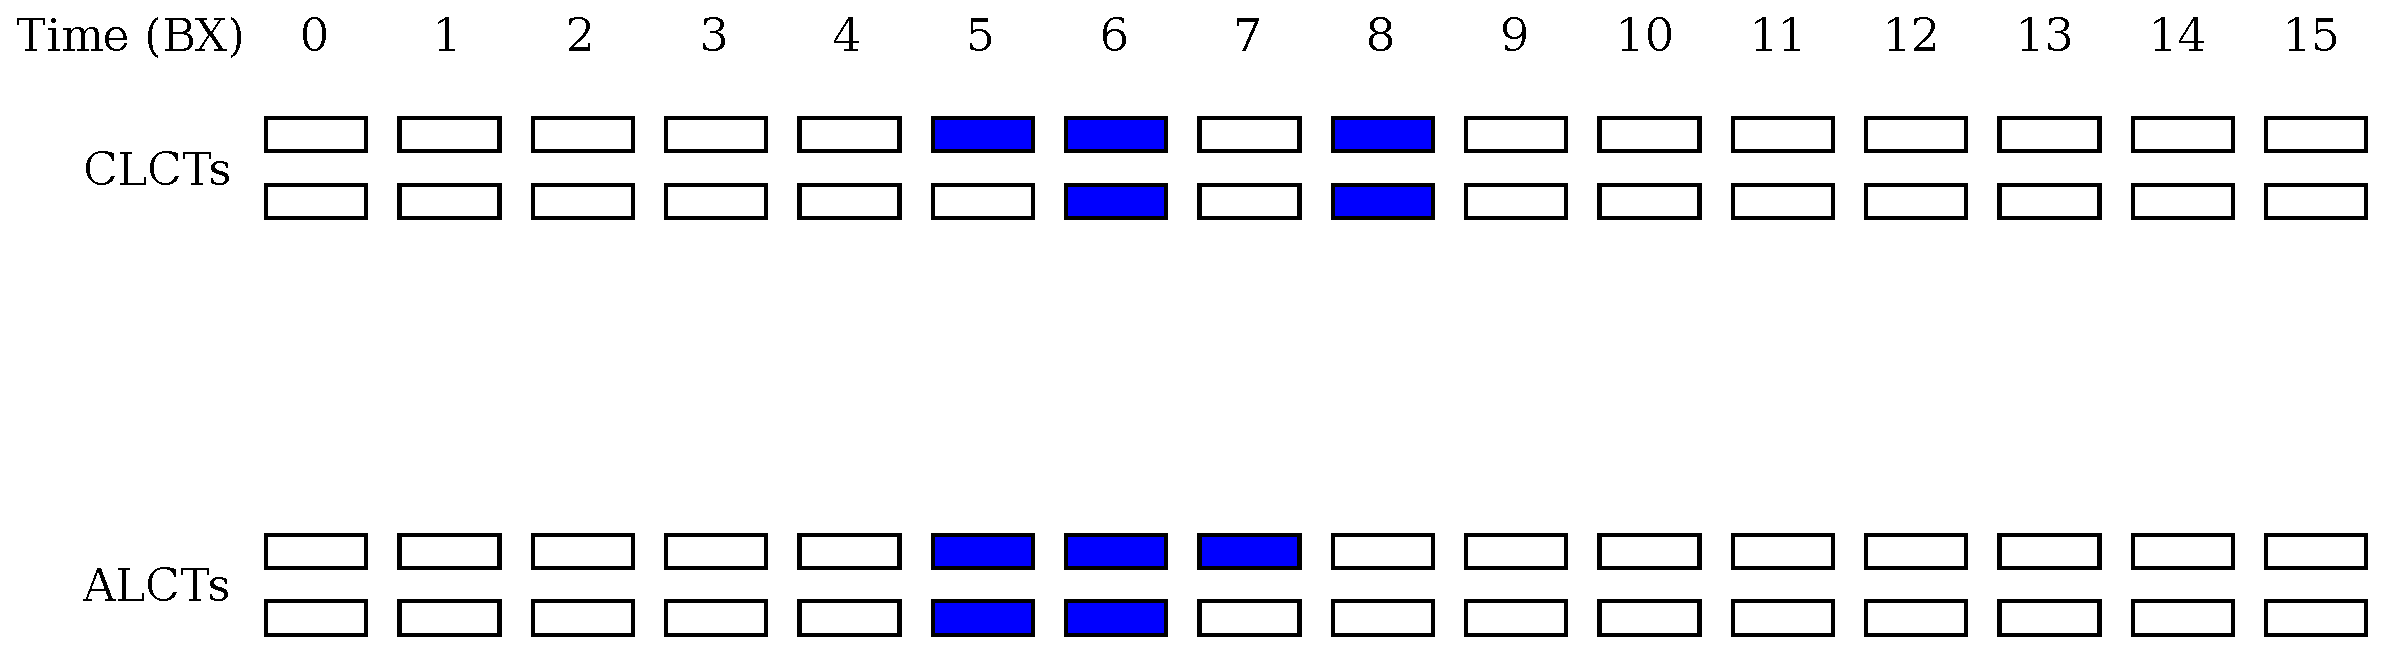
\includegraphics[width=0.7\linewidth]{figures/clcts_alcts.pdf}
                \caption{Example of CLCTs and ALCTs received by OTMB.}
                \label{fig:clcts_alcts}
        \end{center}
\end{figure}

There are two approaches to CLCT and ALCT correlation: CLCT-centric and ALCT-centric. We will introduce the former below and discuss the latter later among OTMB level improvements.

CLCT-centric CLCT and ALCT correlation (see Fig.~\ref{fig:clct_alcts}):
\begin{itemize}
    \item Loop over CLCT BXs from BX = 0 to BX = 15
    \item For CLCT BX = B with at least one valid CLCT:
    \begin{itemize}
        \item Loop over ALCT BXs from BX = B-3 to BX = B+3
        \item Find the first ALCT BX in the matching window with at least one valid ALCT and not marked as used before
        \begin{itemize}
            \item Correlate CLCTs and ALCTs in matching ALCT and CLCT BXs
            \item Mark ALCT BX as used
            \item Proceed to next CLCT BX
        \end{itemize}
    \end{itemize}
\end{itemize}

\begin{figure}[tbh]
        \begin{center}
                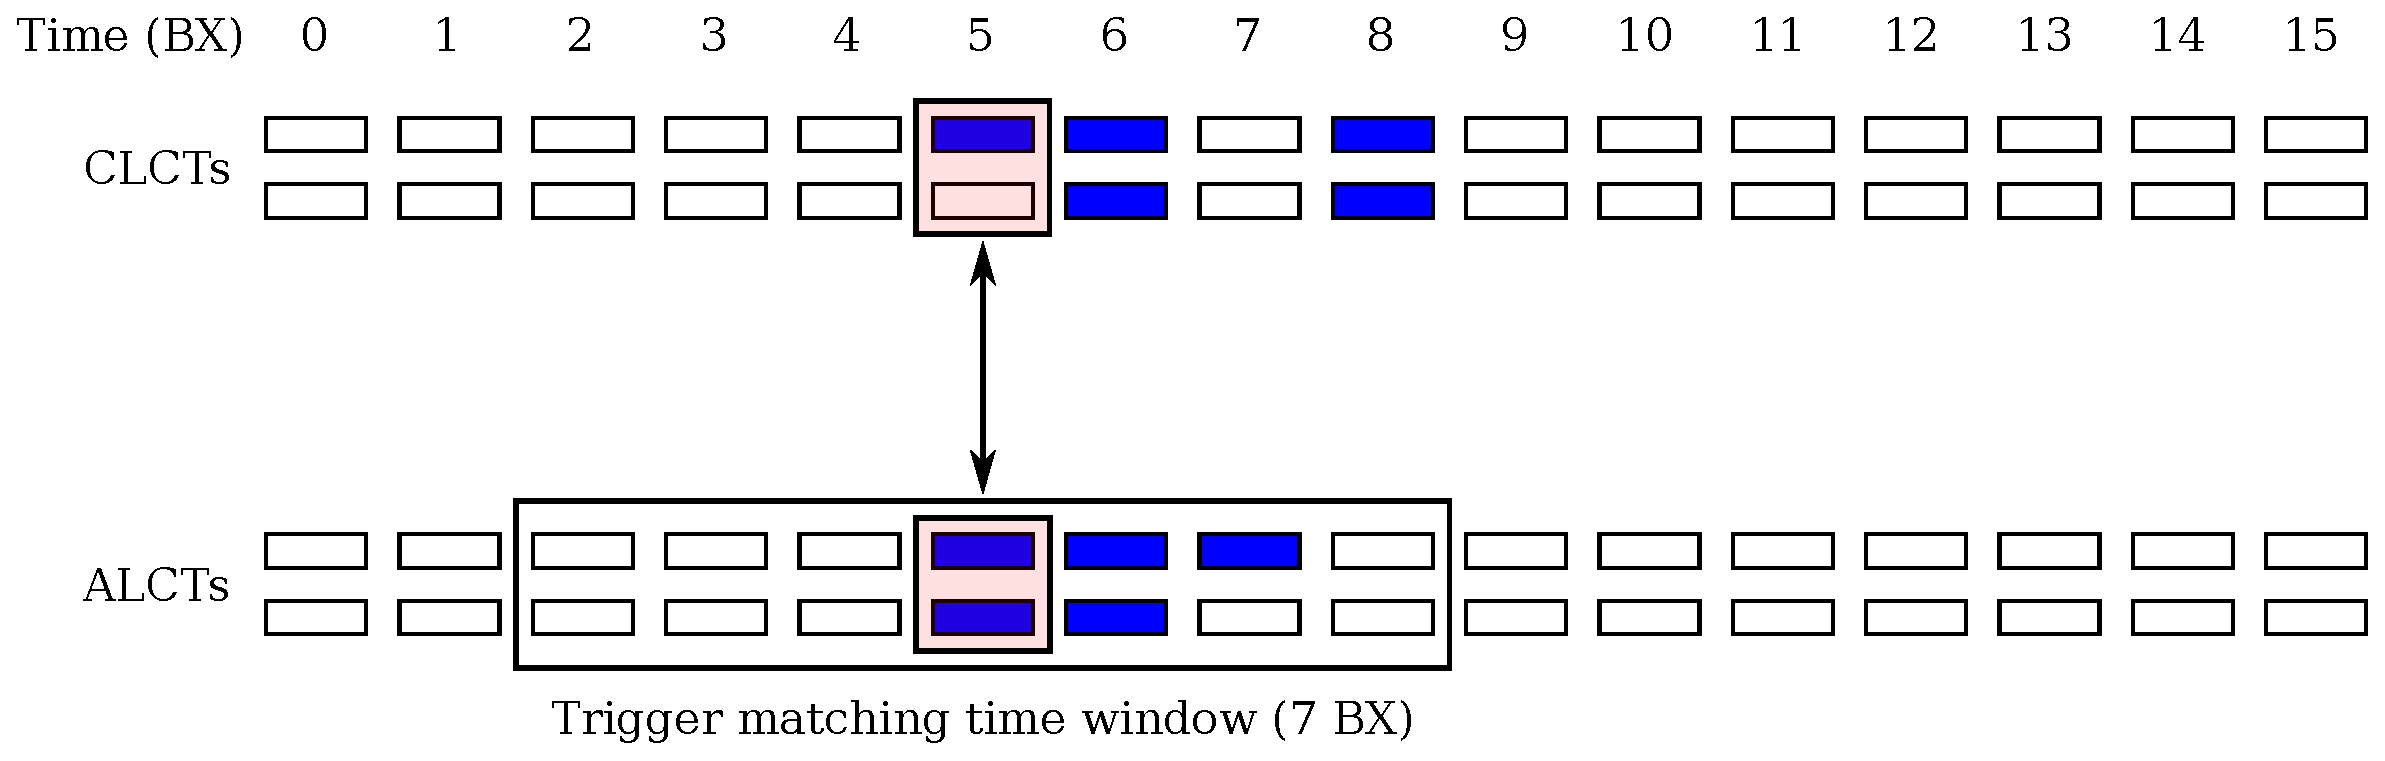
\includegraphics[width=0.7\linewidth]{figures/clct_alcts.pdf}
                \caption{CLCT-centric CLCT and ALCT correlation.}
                \label{fig:clct_alcts}
        \end{center}
\end{figure}

The results of such a correlation are shown on Fig.~\ref{fig:clct_alcts_end}.

\begin{figure}[tbh]
        \begin{center}
                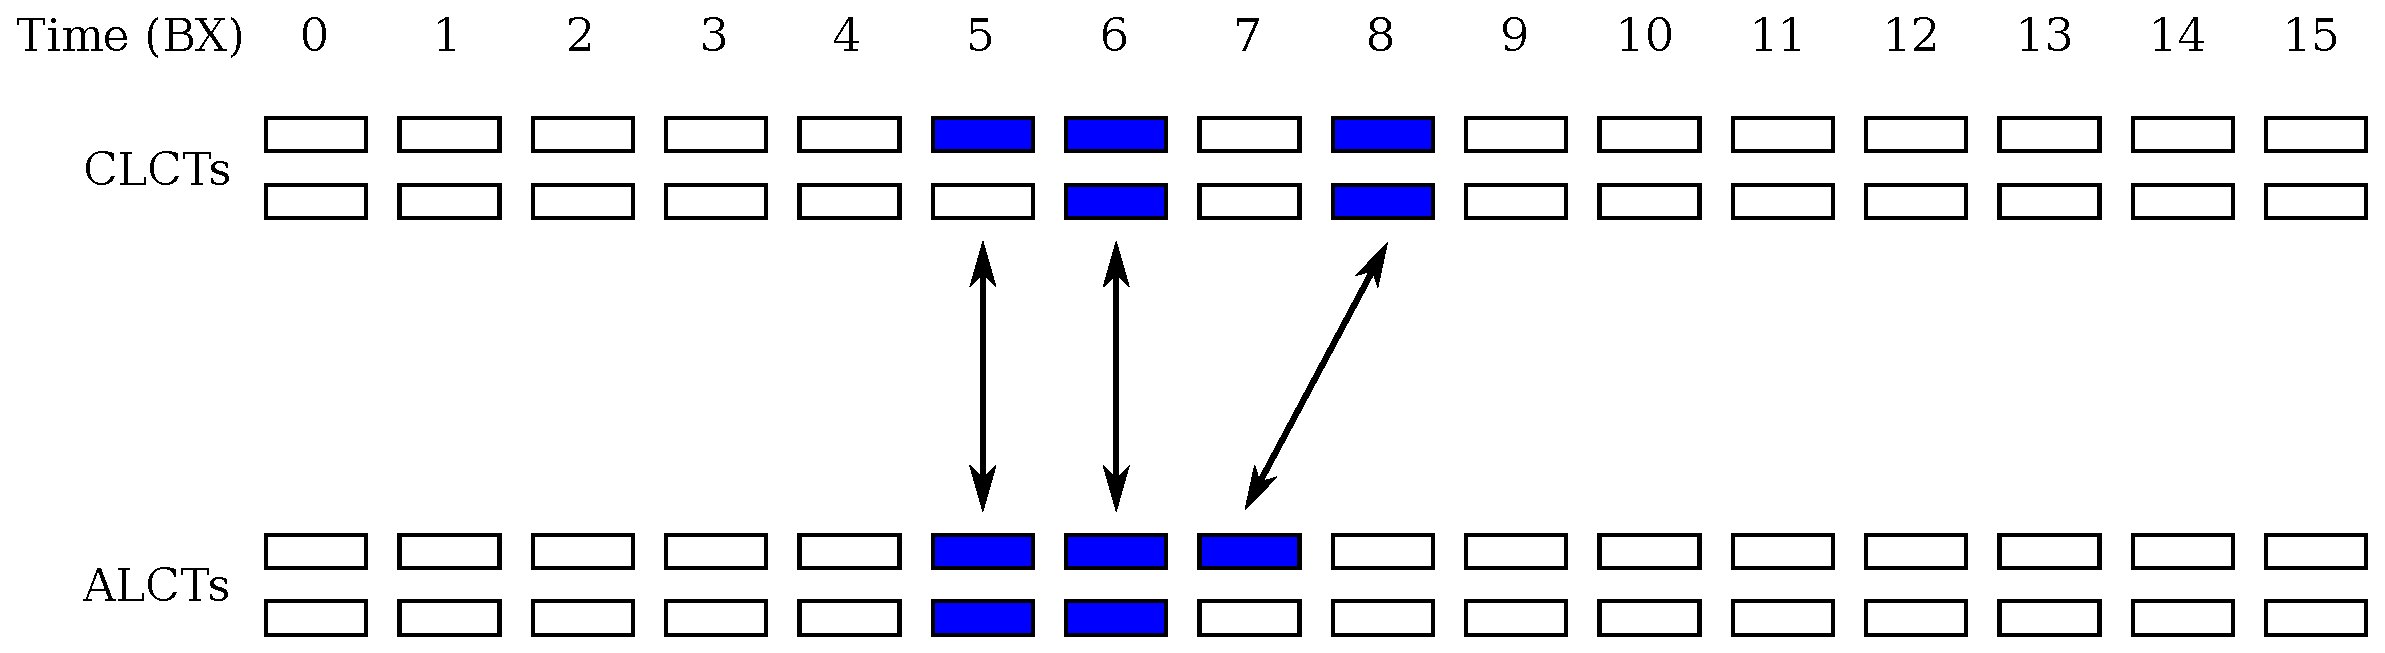
\includegraphics[width=0.7\linewidth]{figures/clct_alcts_end.pdf}
                \caption{Result of CLCT-centric CLCT and ALCT correlation.}
                \label{fig:clct_alcts_end}
        \end{center}
\end{figure}

By default, LCTs are constructed only from valid CLCTs and ALCTs, but we may optionally allow construction of ALCT-less or CLCT-less LCTs.

If there are no ALCT BXs with at least one valid ALCT in the watching window and ALCT-less LCTs are allowed, construct LCTs from valid CLCTs in the current CLCT BX (see example on Fig.~\ref{fig:clct_alcts_alctless} with results on Fig.~\ref{fig:clct_alcts_alctless_end}).

\begin{figure}[tbh]
        \begin{center}
                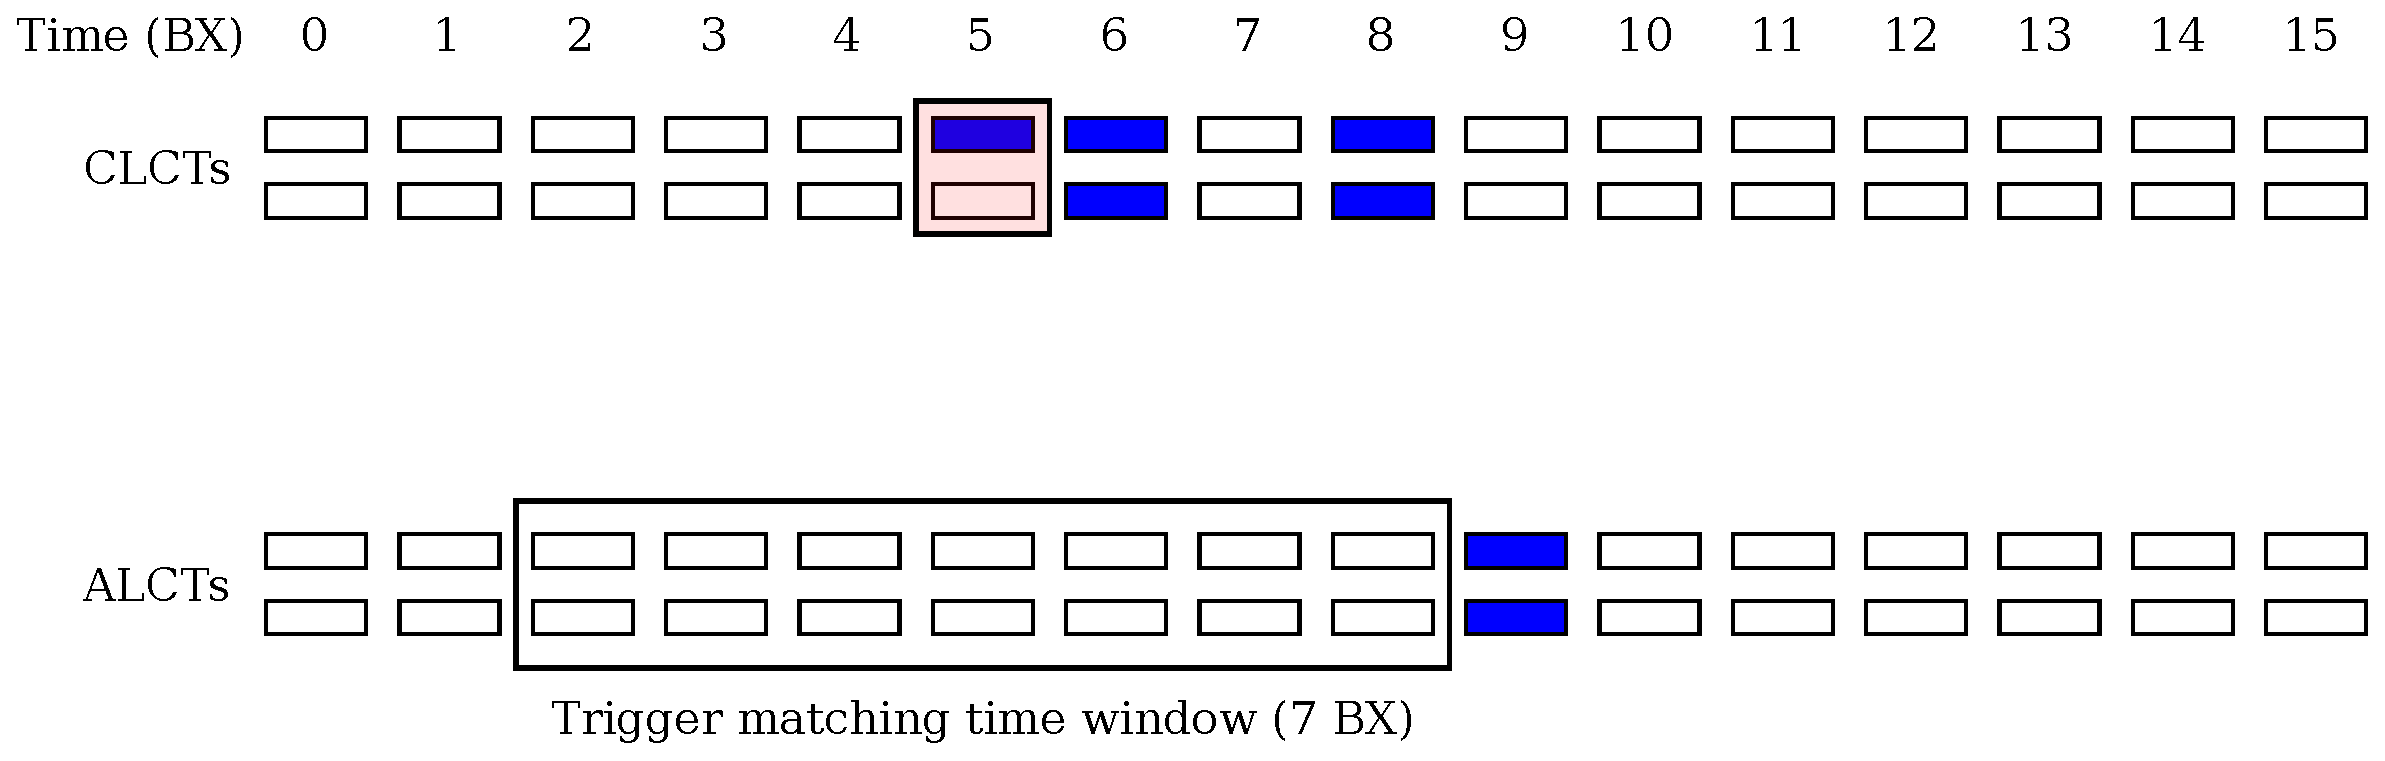
\includegraphics[width=0.7\linewidth]{figures/clct_alcts_alctless.pdf}
                \caption{Example of construction of ALCT-less LCTs.}
                \label{fig:clct_alcts_alctless}
        \end{center}
\end{figure}

\begin{figure}[tbh]
        \begin{center}
                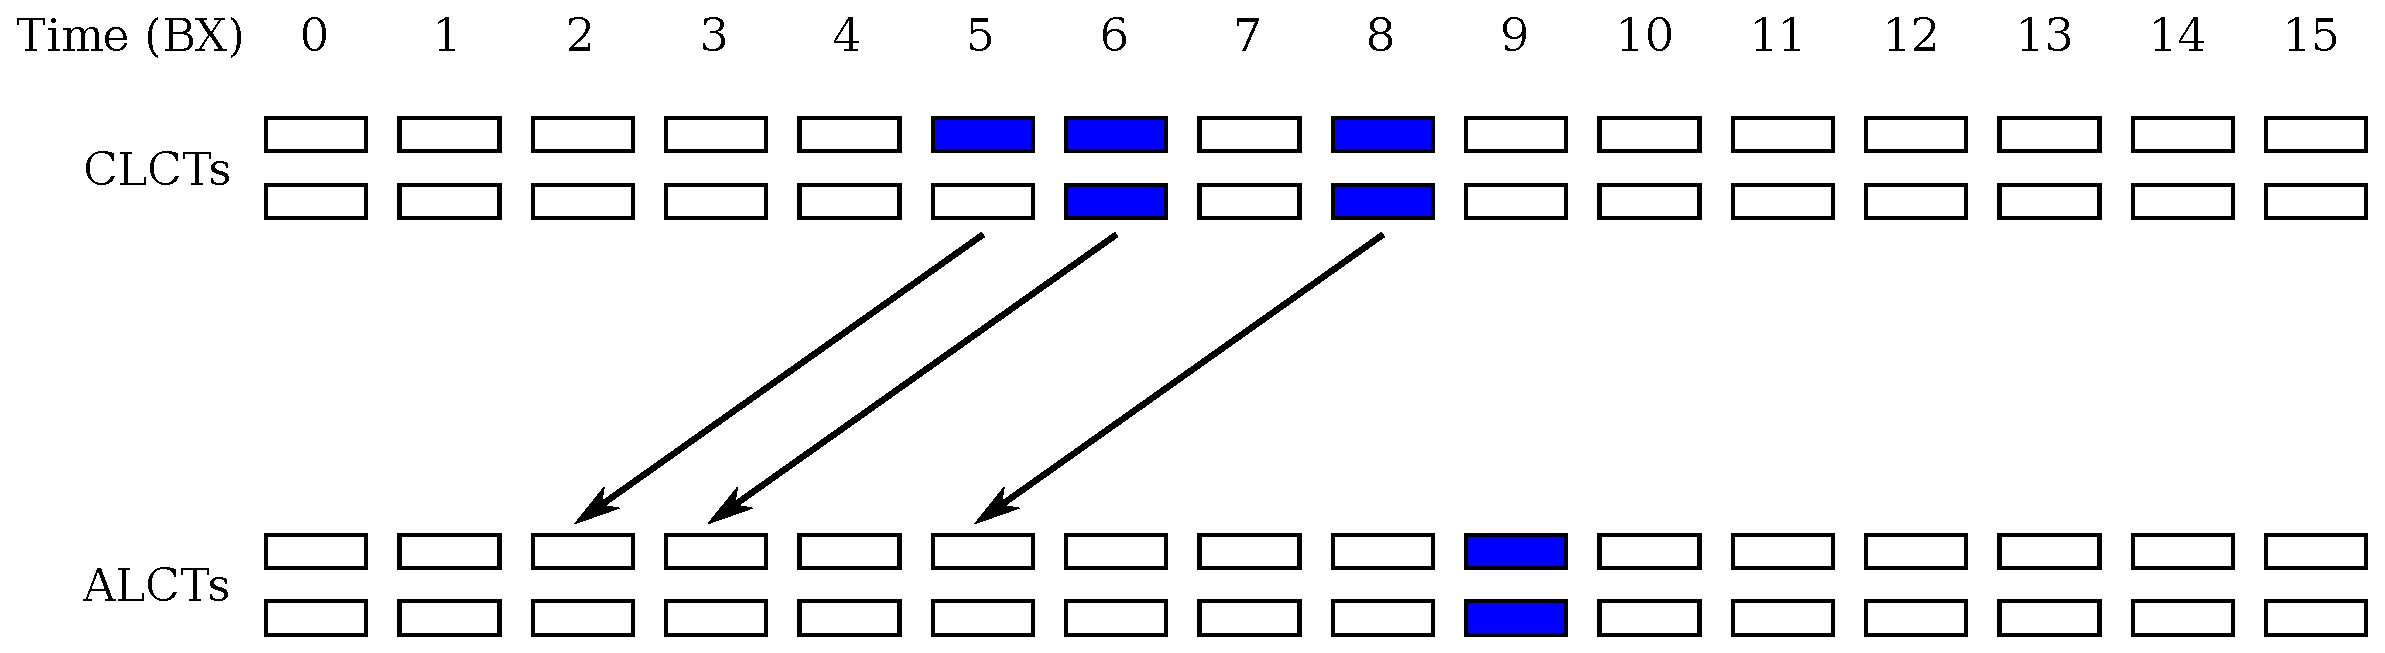
\includegraphics[width=0.7\linewidth]{figures/clct_alcts_alctless_end.pdf}
                \caption{Results of construction of ALCT-less LCTs.}
                \label{fig:clct_alcts_alctless_end}
        \end{center}
\end{figure}

If there are no valid CLCTs in the current CLCT BX and CLCT-less LCTs are allowed (see example on Fig.~\ref{fig:clct_alcts_clctless} with results on Fig.~\ref{fig:clct_alcts_clctless_end}):
\begin{itemize}
    \item Find first ALCT BX in the matching window with at least one valid ALCT and not marked as used before;
    \item Construct LCTs from valid ALCTs in that ALCT BX.
\end{itemize}

\begin{figure}[tbh]
        \begin{center}
                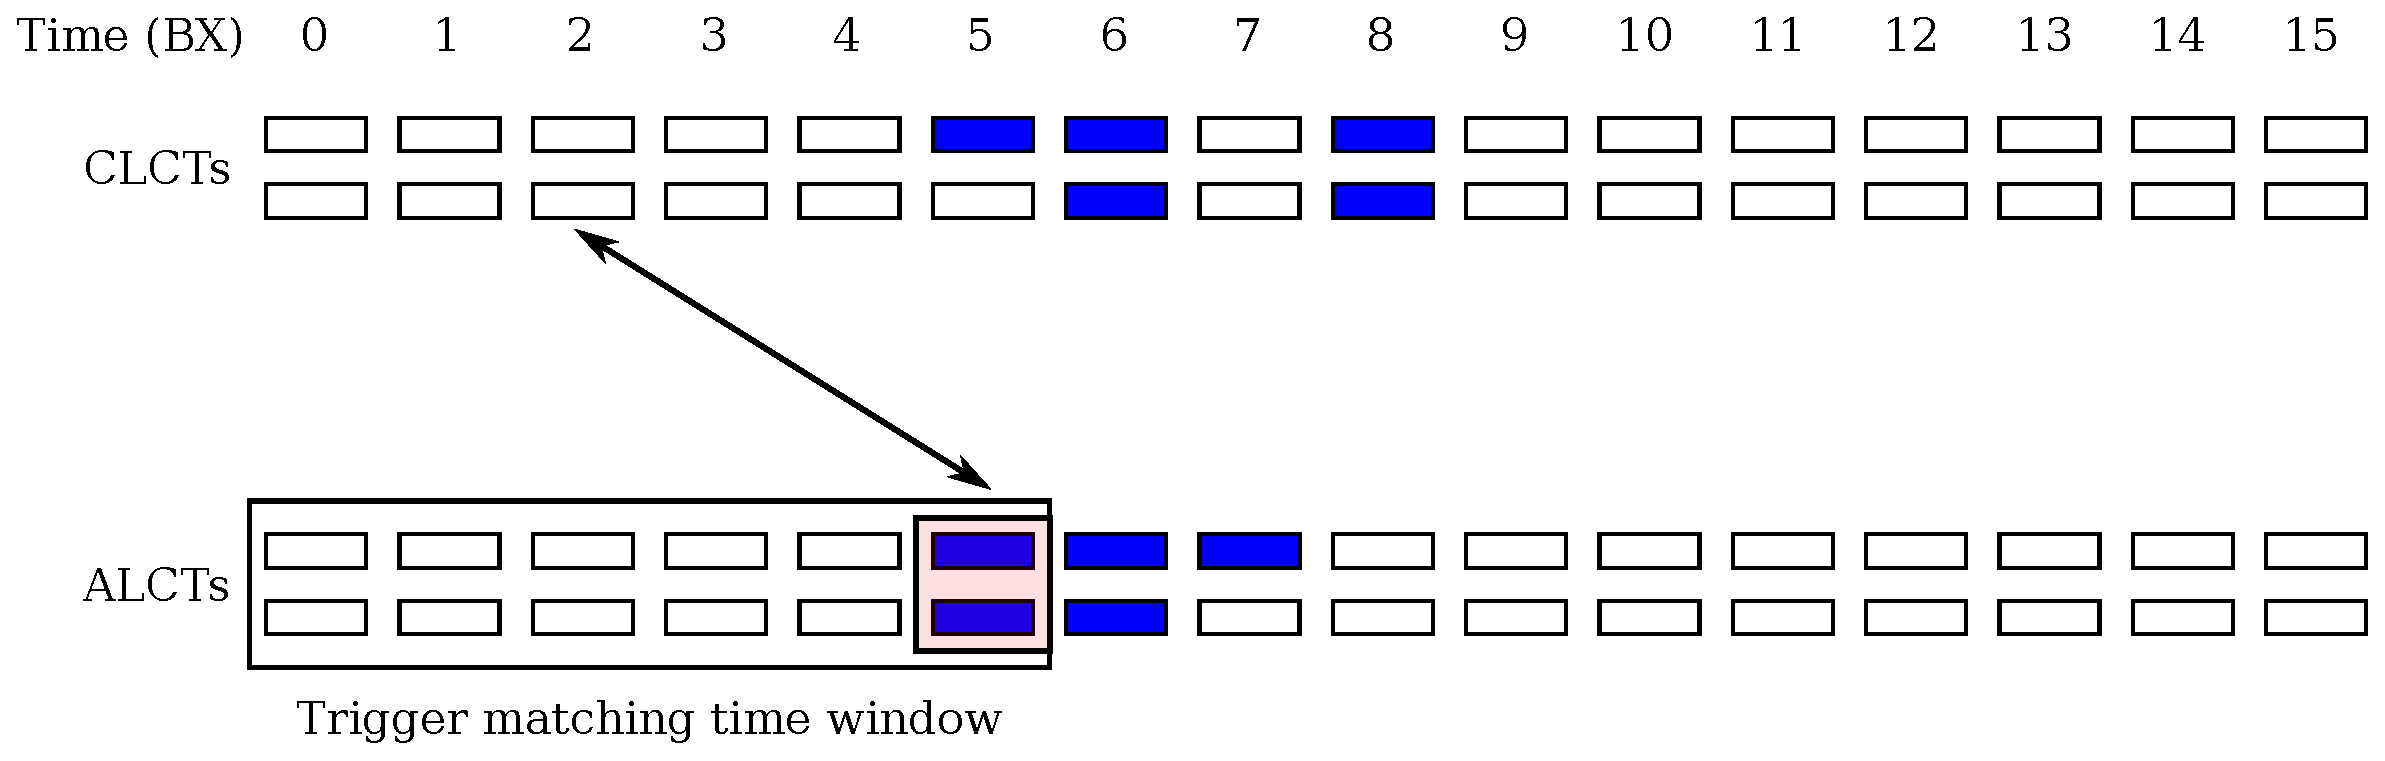
\includegraphics[width=0.7\linewidth]{figures/clct_alcts_clctless.pdf}
                \caption{Example of construction of CLCT-less LCTs.}
                \label{fig:clct_alcts_clctless}
        \end{center}
\end{figure}

\begin{figure}[tbh]
        \begin{center}
                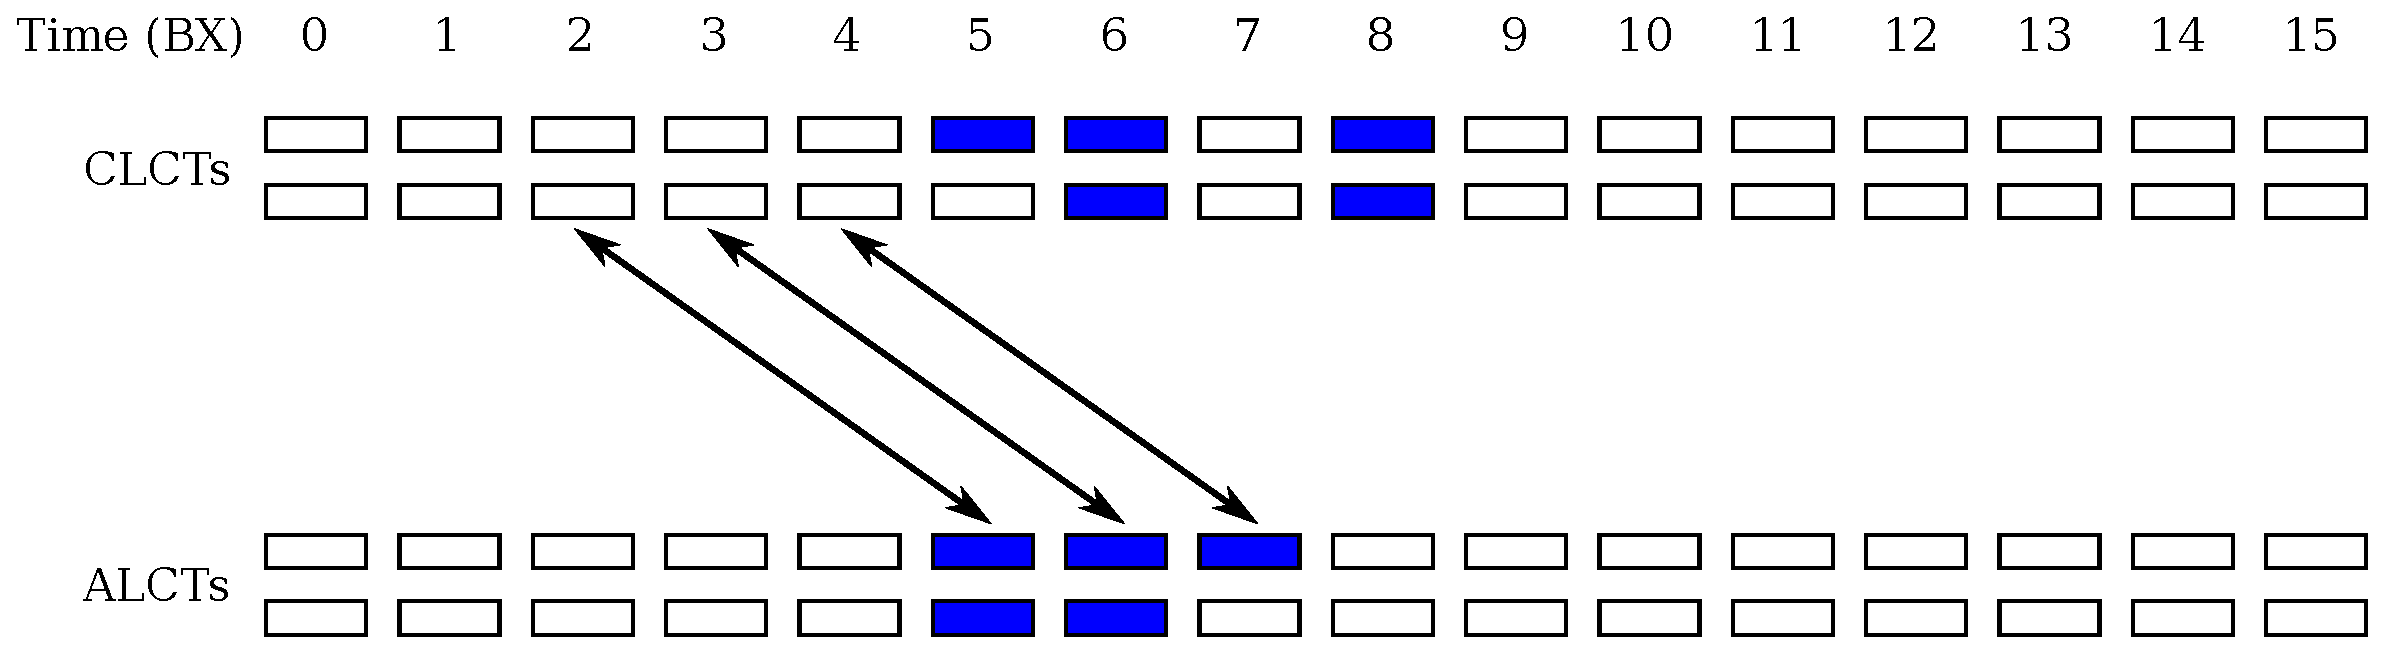
\includegraphics[width=0.7\linewidth]{figures/clct_alcts_clctless_end.pdf}
                \caption{Results of construction of CLCT-less LCTs.}
                \label{fig:clct_alcts_clctless_end}
        \end{center}
\end{figure}

When we use default behavior, where LCTs are constructed only from valid CLCTs and ALCTs, the ideal case is when in matching BXs number of valid CLCTs is equal to number of valid ALCTs (see top two examples on Fig.~\ref{fig:clct_alct_corr}).

\begin{figure}[tbh]
        \begin{center}
                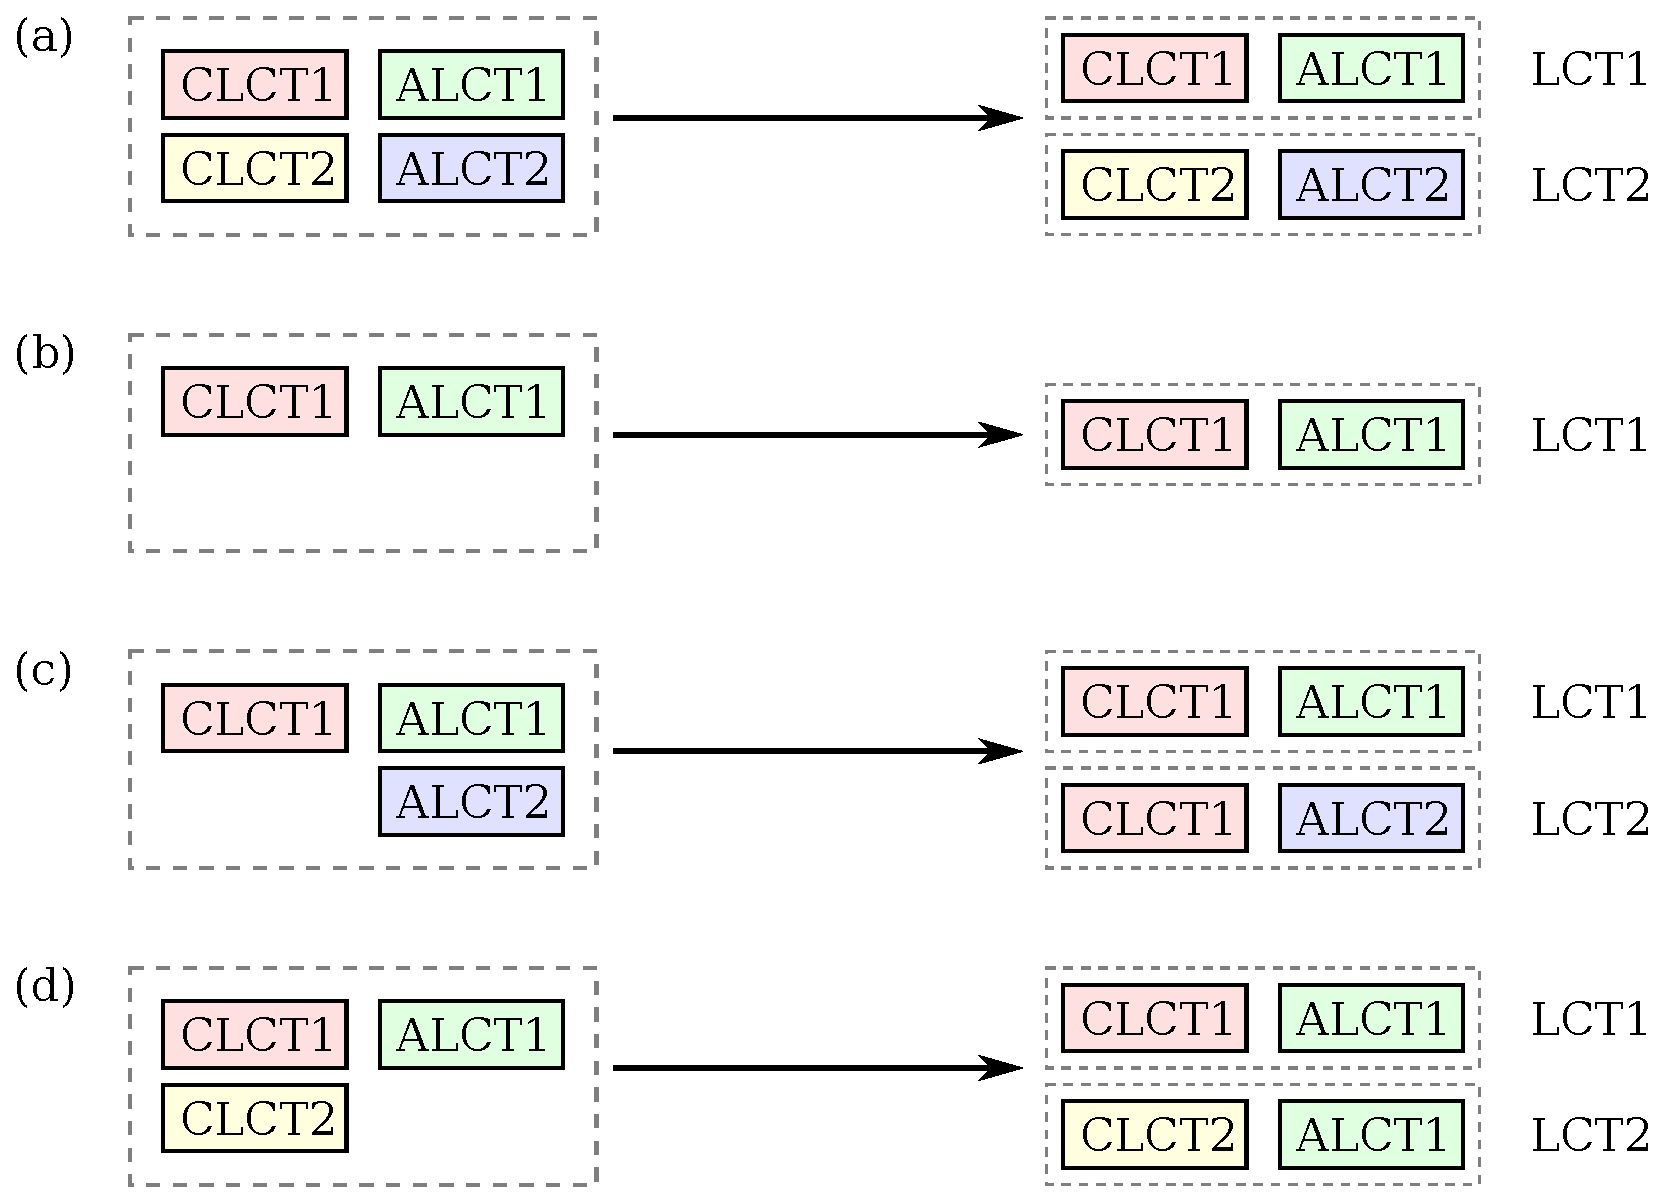
\includegraphics[width=0.7\linewidth]{figures/clct_alct_corr.pdf}
                \caption{Construction of LCTs.}
                \label{fig:clct_alct_corr}
        \end{center}
\end{figure}

But when, for example, there is only one valid CLCT and two valid ALCTs, we make the second valid CLCT from the first, analogously, when there are two valid CLCTs and only one valid ALCT (see bottom two examples on Fig.~\ref{fig:clct_alct_corr}).

\newpage
\subsection{Sofware Emulation of TMB Level Improvements}

\subsubsection{Decreased Trigger Matching Window}

Decrease size of trigger matching time window from 7 BXs to 3 BXs (see Fig.~\ref{fig:clct_alcts_short_window}).

\begin{figure}[tbh]
        \begin{center}
                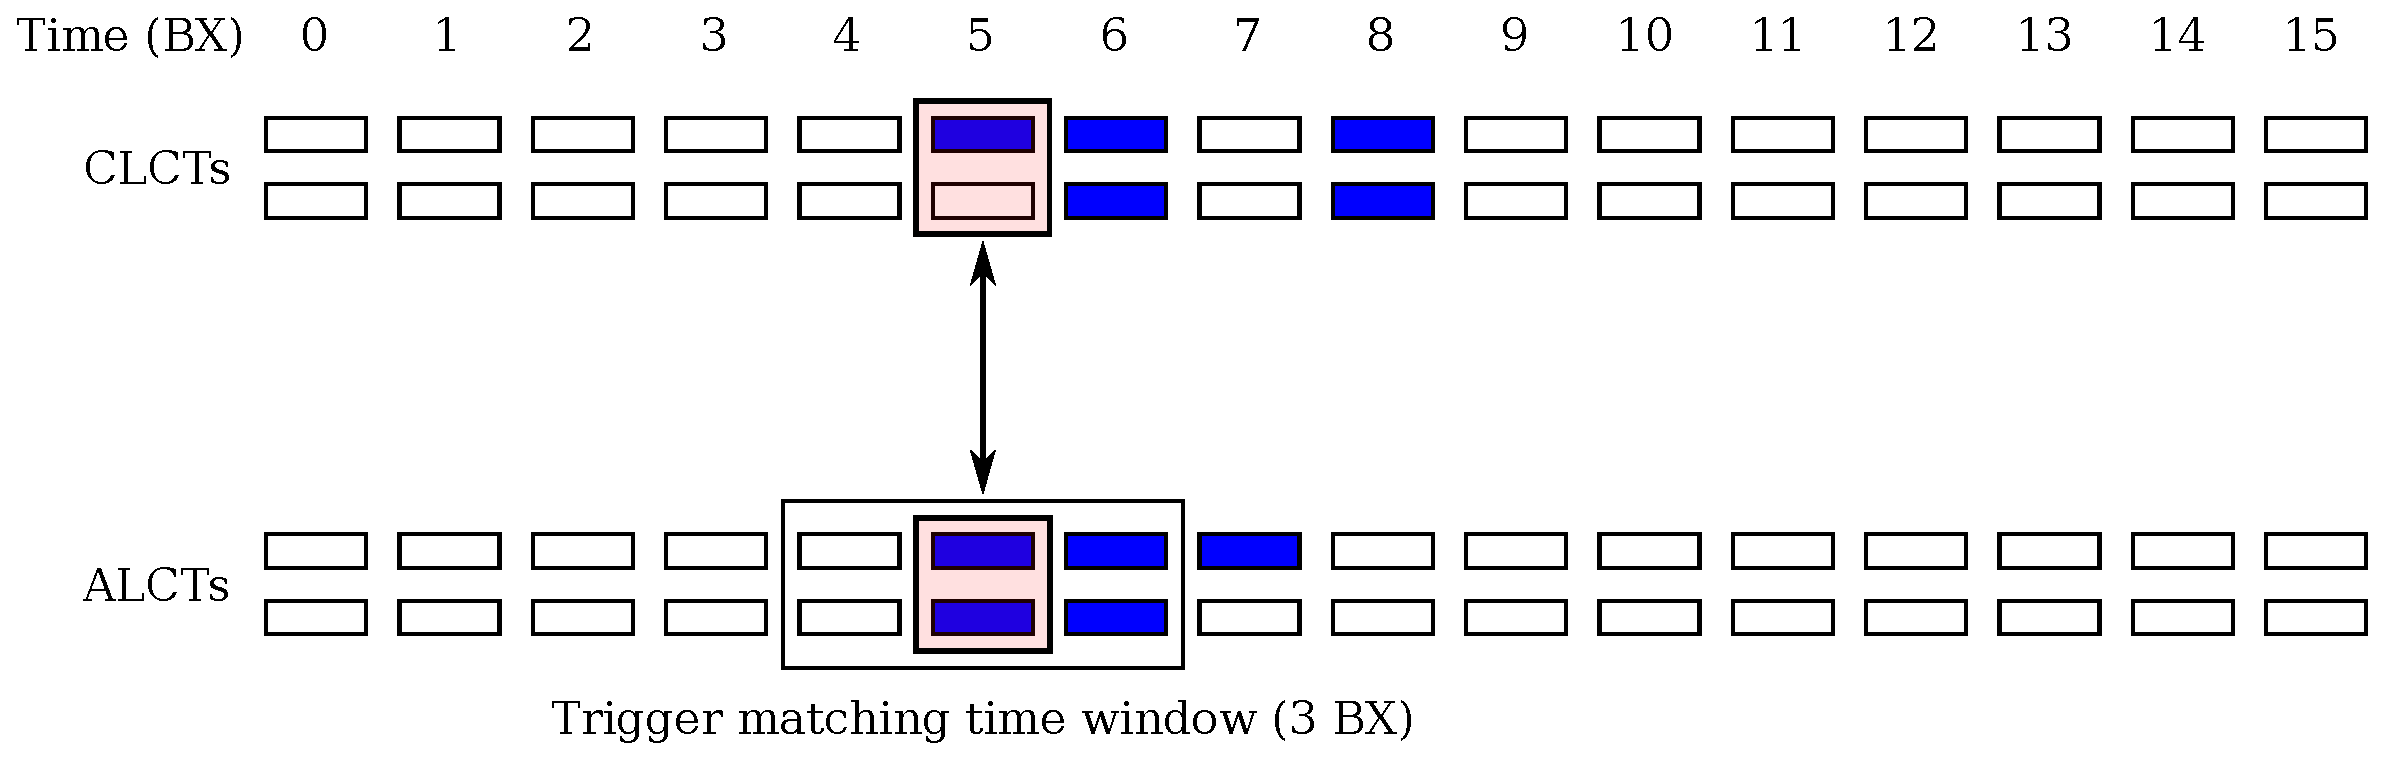
\includegraphics[width=0.98\linewidth]{figures/clct_alcts_short_window.pdf}
                \caption{Decreased trigger matching window.}
                \label{fig:clct_alcts_short_window}
        \end{center}
\end{figure}

The following modifications in configuration are related to this improvement:
\begin{itemize}
    \item matchTrigWindowSize: 7BX to 3BX
\end{itemize}

\subsubsection{ALCT-centric ALCT and CLCT Correlation}

Switch from CLCT-centric matching to ALCT-centric matching (see Fig.~\ref{fig:alct_clcts}).

\textcolor{red}{CLCT-centric matching}
\begin{itemize}
    \item Loop over CLCT BXs from BX = 0 to BX = 15
    \item For CLCT BX = B with at least one valid CLCT:
    \begin{itemize}
        \item Loop over ALCT BXs from BX = B-3 to BX = B+3
    \end{itemize}
\end{itemize}
\textcolor{blue}{ALCT-centric matching}
\begin{itemize}
    \item Loop over ALCT BXs from BX = 0 to BX = 15
    \item For ALCT BX = B with at least one valid ALCT:
    \begin{itemize}
        \item Loop over CLCT BXs from BX = B-3 to BX = B+3
    \end{itemize}
\end{itemize}

\begin{figure}[tbh]
        \begin{center}
                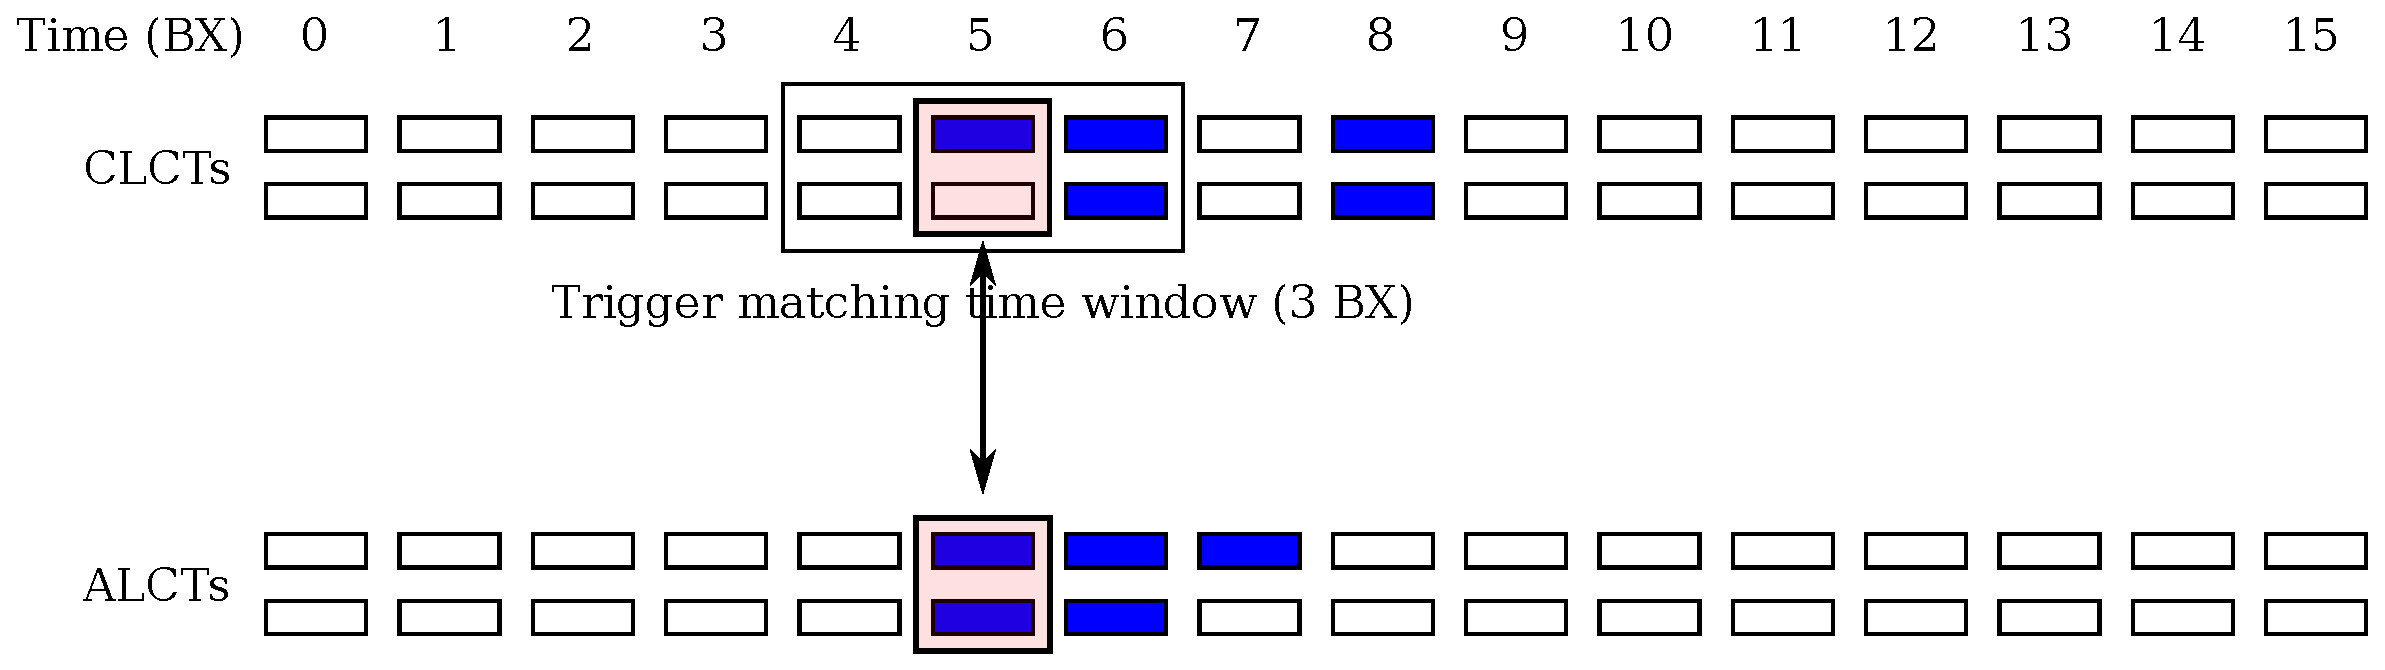
\includegraphics[width=0.98\linewidth]{figures/alct_clcts.pdf}
                \caption{ALCT-centric ALCT anc CLCT correlation.}
                \label{fig:alct_clcts}
        \end{center}
\end{figure}

The following modifications in configuration are related to this improvement:
\begin{itemize}
    \item clctToAlct: True to False
\end{itemize}

\subsubsection{Reusage of Used ALCTs and CLCTs}

Allow reusage of ALCTs and CLCTs already used during ALCT and CLCT correlation (see Fig.~\ref{fig:reuse_alct_clct}).

\textcolor{red}{Current behavior}:
\begin{itemize}
    \item Drop used CLCTs: do not use them with ALCTs in other ALCT BXs;
    \item Proceed to next ALCT BX after matching ALCTs with earliest CLCT BX with at least one valid CLCT.
\end{itemize}
\textcolor{blue}{New behavior}:
\begin{itemize}
    \item Do not drop used CLCTs: reuse them with ALCTs in other ALCT BXs;
    \item Match ALCTs to CLCTs in all CLCT BXs within matching window.
\end{itemize}

\begin{figure}[tbh]
        \begin{center}
                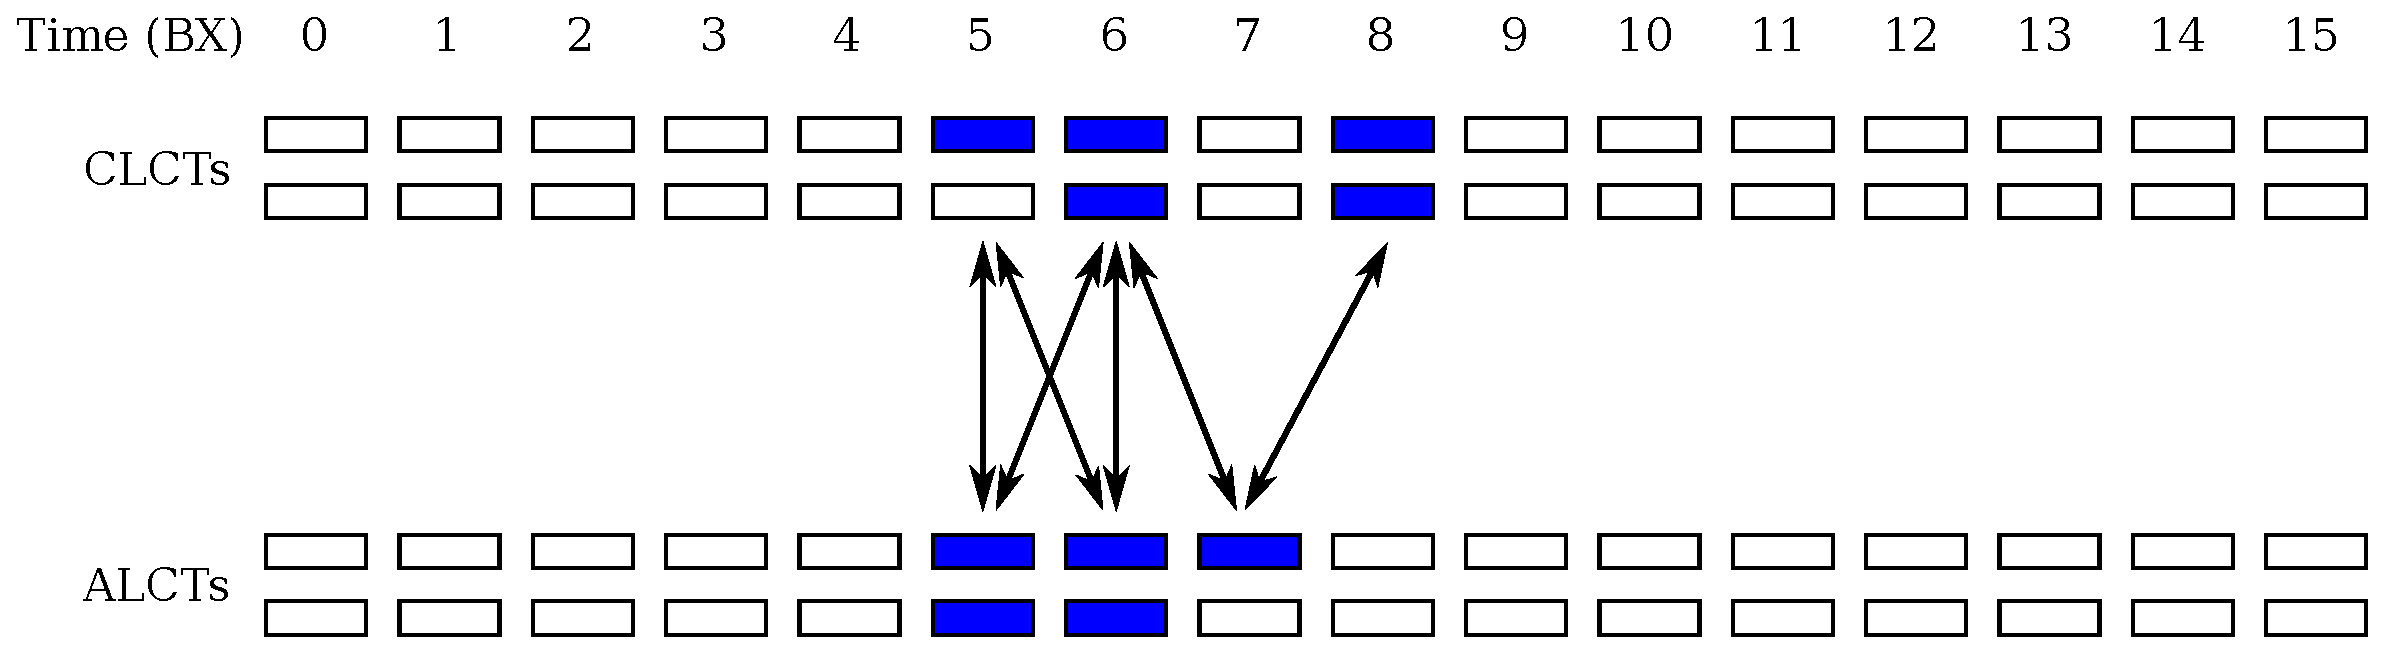
\includegraphics[width=0.98\linewidth]{figures/clct_alcts_end_2.pdf}
                \caption{Reusage of already used ALCTs and CLCTs.}
                \label{fig:reuse_alct_clct}
        \end{center}
\end{figure}

The following modifications in configuration are related to this improvement:
\begin{itemize}
    \item tmbDropUsedClcts: True to False
    \item matchEarliestClctME11Only: True to False
\end{itemize}

\subsubsection{Cross BX Algorithm}

In the situation shown on Fig.~\ref{fig:reuse_alct_clct}, in some given BX = B we can end up having with up to 6 LCTs (made from ALCTs in BX = B and CLCTs in BX = B-1, B, B+2. How do we choose two LCTs to be reported for BX = B?

\textcolor{red}{Current behavior: "cross bx" algorithm is turned off}
\begin{itemize}
    \item Choose two best LCTs with the highest quality
\end{itemize}
\textcolor{blue}{New behavior: "cross bx algorithm"}
\begin{itemize}
    \item Take LCTs with ALCT BX = B and CLCT BX = B
    \item If we still don't have two LCTs, take best ones with ALCT BX = B-1
    \item If we still don't have two LCTs, take best ones with ALCT BX = B+1
\end{itemize}

The following modifications in configuration are related to this improvement:
\begin{itemize}
    \item tmbCrossBxAlgorithm: 0 to 1
\end{itemize}

\newpage

\subsubsection{Corrected ALCT and CLCT Timing}

Use more robust procedure for assignment of ALCT BX and CLCT BX.

\textcolor{red}{Current behavior}:
\begin{itemize}
    \item Use ALCT and CLCT pretrigger BXs to assign ALCT BX and CLCT BX.
\end{itemize}
\textcolor{blue}{New behavior}:
\begin{itemize}
    \item For each hit in ALCT and CLCT trigger patterns, determine "first BX": BX of original hit before hit stretching over 6 BXs;
    \item For ALCTs, consider hits in key WG = N and two neighbouring WGs: WG = N-1 and WG = N+1;
    \item For CLCTs, consider all hits in the pattern;
    \item Store "first BXs" of these hits in two sorted sets (one for ALCT times and another for CLCT times);
    \item Use median elements in these sets to assign ALCT BX and CLCT BX.
\end{itemize}

The following modifications in configuration are related to this improvement:
\begin{itemize}
    \item alctUseCorrectedBx: False to True
    \item clctUseCorrectedBx: False to True
\end{itemize}

\subsubsection{Reading out more LCTs}

[I'm not sure I completely understand the meaning of this improvement]

\textcolor{red}{Current behavior}
\begin{itemize}
    \item In digi$\rightarrow$raw step, LCTs have to be packed into the TMB header, and currently there is room just for two
    \item Take LCTs only from earliest BX in L1A readout with at least one LCT
\end{itemize}
\textcolor{blue}{New behavior}
\begin{itemize}
    \item Take LCTs from the whole L1A readout (from BX = 5 to BX = 11)
\end{itemize}

The following modifications in configuration are related to this improvement:
\begin{itemize}
    \item tmbReadoutEarliest2: True to False
\end{itemize}


\subsection{Results of Improvements of the ALCT and CLCT Matching}

Improvements on the level of TMB are related to the following configuration parameters (see Sec.~\ref{sec:TMB_conf}):
\begin{itemize}
	\item matchTrigWindowSize: 7BX to 3BX;
	\item tmbReadoutEarliest2: True to False;
	\item alctUseCorrectedBx: False to True
	\item clctUseCorrectedBx: False to True;
	\item clctToAlct: True to False;
	\item tmbDropUsedClcts and matchEarliestClctME11Only: True to False;
	\item tmbCrossBxAlgorithm: 0 to 1.
\end{itemize}

Fig.~\ref{fig:TMB_improvements_LCT_recoEff} shows reconstruction efficiency of a good LCT in ME1/1 station versus pseudorapidity of the simulated muon for different L1 configurations. The good LCT is defined as LCT consisted of a good ALCT and a good CLCT.

The major improvement in LCT reconstruction efficiency comes from:
\begin{itemize}
	\item changing the size of a window where ALCTs and CLCTs are read out for further correlation between each other;
	\item stopping to read out only the first two CLCTs;
	\item stopping to drop used CLCTs;
	\item stopping to match only to the earliest CLCT.
\end{itemize}

The effects on the efficiency improvements are more evident if we divide the whole ME1/1 chamber into three different sections by eta:
\begin{itemize}
        \item from $ \eta = 1.65 $ to $ \eta = 2.0 $ to cover the ME1/1b chamber alone;
        \item from $ \eta = 2.0 $ to $ \eta = 2.2 $ to cover the gap between ME1/1a and ME1/1b;
        \item from $ \eta = 2.2 $ to $\eta = 2.45 $ to cover the ME1/1a chamber alone;
\end{itemize}

The effects on the efficiency for each one of the TMB improvment in the main $\eta$ partitions defined above are summarized in Tab.~\ref{eff_pu140} for PU140 and in Tab.~\ref{eff_pu50} for PU50. A more detailed study comparing each improvment over the whole $\eta$ range for the ME1/1 chamber can be found in Appendix.

\begin{figure}[p]
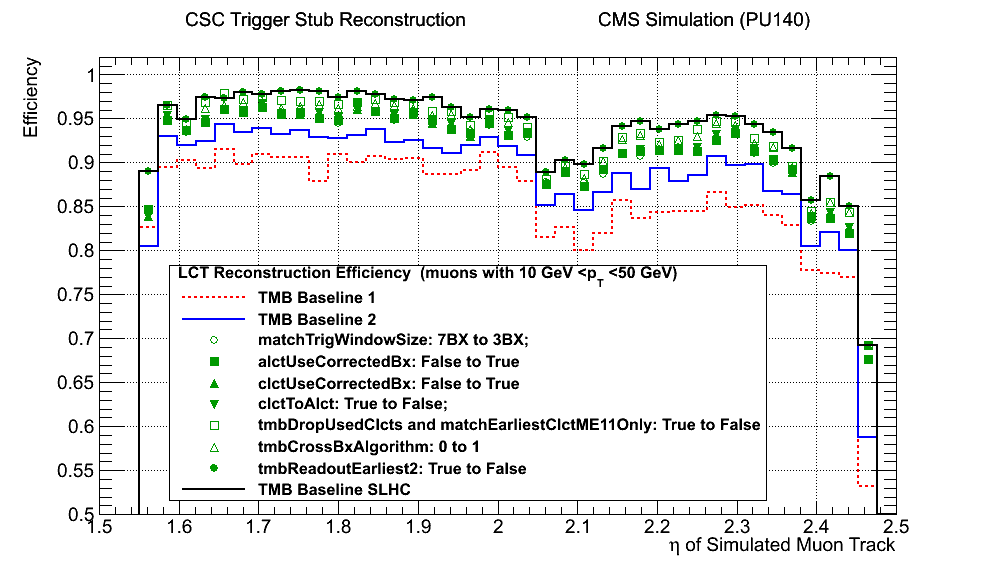
\includegraphics[width=0.98\textwidth]{figures/TMB_improvements_LCT_recoEff.png}
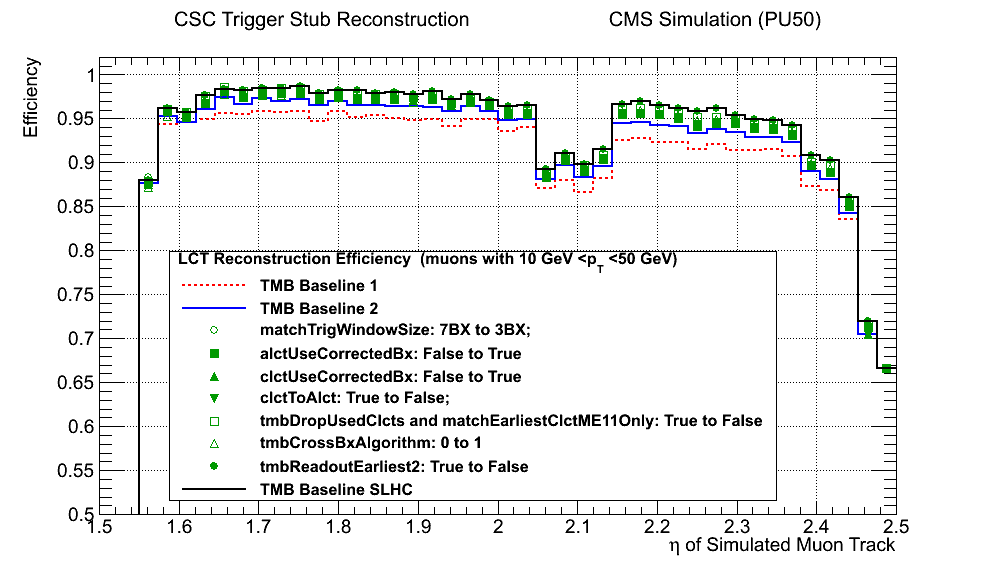
\includegraphics[width=0.98\textwidth]{figures/TMB_improvements_LCT_recoEff_PU50.png}
\caption{LCT reconstruction efficiency in ME1/1 station for PU140 (top) and PU50 (bottom). Muons with transverse momentum $10$~GeV$<p_T<50$~ GeV are used in the analysis.}
\label{fig:TMB_improvements_LCT_recoEff}
\end{figure}

\begin{table}[h]
\begin{tabular}{| p{7.4 cm}| c | c | c | c | c | c | }
\hline
\multirow{2}{*}{Improvment} & \multicolumn {2}{|c|}{ME1/1b} & \multicolumn{2}{|c|}{Gap Region} & \multicolumn{2}{|c|}{ME1/1a} \\ \cline{2-7}
                            & $\epsilon$ (\%)  & $\delta \epsilon$ & $\epsilon$ (\%) & $\delta \epsilon$ & $\epsilon$ (\%) & $\delta \epsilon$ \\  \hline
TMB Baseline 1 & 89.92 & 0.13 & 82.62 & 0.16 & 82.54 & 0.16 \\ \hline
TMB Baseline 2 & 92.63 & 0.11 & 86.53 & 0.15 & 86.38 & 0.15 \\ \hline
matchTrigWindowsSize: 7BX to 3 BX & 94.38 & 0.09 & 89.27 & 0.13 & 88.97 & 0.13 \\ \hline
alctUseCorrectedBX: False to True & 95.00 & 0.09 & 89.36 & 0.13 & 89.35 &  0.13  \\ \hline 
clctUseCorrectedBX: False to True & 95.01 & 0.09 & 89.37 & 0.13 & 89.36 & 0.13 \\ \hline
clctToAlct: True to False & 95.11 & 0.09 & 89.40 & 0.13 & 80.36 & 0.13 \\ \hline
tmbDropUsedClcts and matchEarliestClctME11Only: False to True & 96.27 & 0.08 & 90.54 & 0.12 & 90.59 & 0.12 \\ \hline
tmbCrossBXAlgorithm: 0 to 1 & 95.69 & 0.09 & 90.24 & 0.13 & 90.33 & 0.13 \\ \hline
tmbReadoutEarliest2: True to False & 97.00 & 0.07 & 91.65 & 0.12 & 91.97 & 0.12 \\ \hline
TMB Baseline SLHC & 97.00 & 0.07 & 91.65 & 0.12 & 91.97 & 0.12 \\ \hline
\end{tabular}
\caption{LCT reconstruction efficiencies in ME1/1 station after individual improvements in algorithm for PU140. Muons with transverse momentum $10$~GeV$<p_T<50$~ GeV are used in the analysis.}
\label{eff_pu140}
\end{table}

\begin{table}[h]
\begin{tabular}{| p{7.4 cm}| c | c | c | c | c | c | }
\hline
\multirow{2}{*}{Improvment} & \multicolumn {2}{|c|}{ME1/1b} & \multicolumn{2}{|c|}{Gap Region} & \multicolumn{2}{|c|}{ME1/1a} \\ \cline{2-7}
                            & $\epsilon$ (\%)  & $\delta \epsilon$ & $\epsilon$ (\%) & $\delta \epsilon$ & $\epsilon$ (\%) & $\delta \epsilon$ \\  \hline
TMB Baseline 1 & 94.95 & 0.09 & 89.18 & 0.13 & 90.38 & 0.13 \\ \hline
TMB Baseline 2 & 96.32 & 0.08 & 90.74 & 0.12 & 91.78 & 0.12 \\ \hline
matchTrigWindowsSize: 7BX to 3 BX & 97.13 & 0.07 & 91.72 & 0.12 & 92.91 & 0.11 \\ \hline
alctUseCorrectedBX: False to True & 97.13 & 0.07 & 91.80 & 0.12 & 93.00 & 0.11 \\ \hline
clctUseCorrectedBX: False to True & 97.03 & 0.07 & 91.80 & 0.12 & 93.06 & 0.11 \\ \hline
clctToAlct: True to False & 97.03 & 0.07 & 91.80 & 0.12 & 93.06 & 0.11 \\ \hline
tmbDropUsedClcts and matchEarliestClctME11Only: False to True & 97.52 & 0.07 & 92.23 & 0.11 & 93.61 & 0.10 \\ \hline
tmbCrossBXAlgorithm: 0 to 1 & 97.03 & 0.07 & 91.86 & 0.12 & 93.39 & 0.11 \\ \hline
tmbReadoutEarliest2: True to False & 97.69 & 0.06 & 92.62 & 0.11 & 94.07 & 0.10 \\ \hline 
TMB Baseline SLHC & 97.69 & 0.06 & 92.62 & 0.11 & 94.07 & 0.10 \\ \hline 
\end{tabular}
\caption{LCT reconstruction efficiencies in ME1/1 station after individual improvements in algorithm for PU50. Muons with transverse momentum $10$~GeV$<p_T<50$~ GeV are used in the analysis.}
\label{eff_pu50}
\end{table}

\clearpage

% >> acknowledgements (for journal papers)
% Please include the latest version from https://twiki.cern.ch/twiki/bin/viewauth/CMS/Internal/PubAcknow.
%\section*{Acknowledgements}
% ack-text

%% **DO NOT REMOVE BIBLIOGRAPHY**
\bibliography{auto_generated}   % will be created by the tdr script.
%% Customizable fields and text areas start with % >> below.
% Lines starting with the comment character (%) are normally removed before release outside the collaboration, but not those comments ending lines

% svn info. These are modified by svn at checkout time.
% The last version of these macros found before the maketitle will be the one on the front page,
% so only the main file is tracked.
% Do not edit by hand!
\RCS$Revision: 315441 $
\RCS$HeadURL: svn+ssh://pakhotin@svn.cern.ch/reps/tdr2/notes/DN-13-022/trunk/DN-13-022.tex $
\RCS$Id: DN-13-022.tex 315441 2015-12-17 00:18:24Z pakhotin $
%%%%%%%%%%%%% local definitions %%%%%%%%%%%%%%%%%%%%%
% This allows for switching between one column and two column (cms@external) layouts
% The widths should  be modified for your particular figures. You'll need additional copies if you have more than one standard figure size.
\newlength\cmsFigWidth
\ifthenelse{\boolean{cms@external}}{\setlength\cmsFigWidth{0.85\columnwidth}}{\setlength\cmsFigWidth{0.4\textwidth}}
\ifthenelse{\boolean{cms@external}}{\providecommand{\cmsLeft}{top}}{\providecommand{\cmsLeft}{left}}
\ifthenelse{\boolean{cms@external}}{\providecommand{\cmsRight}{bottom}}{\providecommand{\cmsRight}{right}}
%%%%%%%%%%%%%%%  Title page %%%%%%%%%%%%%%%%%%%%%%%%
\cmsNoteHeader{DN-13-022} % This is over-written in the CMS environment: useful as preprint no. for export versions
% >> Title: please make sure that the non-TeX equivalent is in PDFTitle below
\title{ME1/1 Local Trigger Algorithm \\ for Operation under High Pile-Up Running Conditions}

% >> Authors
%Author is always "The CMS Collaboration" for PAS and papers, so author, etc, below will be ignored in those cases
%For multiple affiliations, create an address entry for the combination
%To mark authors as primary, use the \author* form
%\address[ghent]{Ghent University}
\address[tamu]{Texas A\&M University}
\address[ucla]{University of California, Los Angeles}
\address[ufl]{University of Florida}
\author[tamu]{Sven Dildick}
\author[tamu]{Jose Roberto Dimas Valle}
\author[tamu]{Jason Gilmore}
\author[ucla]{Jay Hauser}
\author[tamu]{Tao Huang}
\author[tamu]{Vadim Khotilovich}
\author[tamu]{Vyacheslav Krutelyov}
\author[ufl]{Alexander Madorsky}
\author[tamu]{Yuriy Pakhotin}
\author[ucla]{Andrew Peck}
\author[tamu]{Alexei Safonov}
\author[tamu]{Aysen Tatarinov}
\author[ucla]{Vyacheslav Valuev}

% >> Date
% The date is in yyyy/mm/dd format. Today has been
% redefined to match, but if the date needs to be fixed, please write it in this fashion.
% For papers and PAS, \today is taken as the date the head file (this one) was last modified according to svn: see the RCS Id string above.
% For the final version it is best to "touch" the head file to make sure it has the latest date.
\date{\today}

% >> Abstract
% Abstract processing:
% 1. **DO NOT use \include or \input** to include the abstract: our abstract extractor will not search through other files than this one.
% 2. **DO NOT use %**                  to comment out sections of the abstract: the extractor will still grab those lines (and they won't be comments any longer!).
% 3. For PASs: **DO NOT use tex macros**         in the abstract: CDS MathJax processor used on the abstract doesn't understand them _and_ will only look within $$. The abstracts for papers are hand formatted so macros are okay.
\abstract{
An important piece of the CMS muon trigger upgrade is developing and maintaining FPGA firmware for new custom electronics - optical trigger mother-board for ME1/1 muon detectors. This firmware uses massively parallel pattern recognition algorithm to find quality muon stubs. An improved local trigger algorithm to perform sophisticated background rejection is developed for operation under high pile-up running conditions. Implementation of the improvements to the algorithm is described. Configuration of the CMS software for the algorithm simulation is specified. Individual effects of the improvements on the ME1/1 local trigger efficiency are quantified and ranked using simulated samples.
}

% >> PDF Metadata
% Do not comment out the following hypersetup lines (metadata). They will disappear in NODRAFT mode and are needed by CDS.
% Also: make sure that the values of the metadata items are sensible and are in plain text:
% (1) no TeX! -- for \sqrt{s} use sqrt(s) -- this will show with extra quote marks in the draft version but is okay).
% (2) no %.
% (3) No curly braces {}.
\hypersetup{%
pdfauthor={Aysen Tatarinov, Yuriy Pakhotin},%
pdftitle={ME1/1 Local Trigger Algorithm for Operation under High Pile-Up Running Conditions},%
pdfsubject={CMS},%
pdfkeywords={LHC, CMS, Muons, CSC, Trigger}}

\maketitle %maketitle comes after all the front information has been supplied
% >> Text
%%%%%%%%%%%%%%%%%%%%%%%%%%%%%%%%  Begin text %%%%%%%%%%%%%%%%%%%%%%%%%%%%%
%% **DO NOT REMOVE THE BIBLIOGRAPHY** which is located before the appendix.
%% You can take the text between here and the bibiliography as an example which you should replace with the actual text of your document.
%% If you include other TeX files, be sure to use "\input{filename}" rather than "\input filename".
%% The latter works for you, but our parser looks for the braces and will break when uploading the document.

\tableofcontents

\newpage
\tracinginput{sections/sec_introduction.tex}
%\section{Introduction}

Muon system is hosted in the steel yokes of the CMS detector~\cite{Chatrchyan:2008aa} and it is divided into a central part (barrel: $|\eta| < 1.2$) with Drift-Tube (DT) detectors and two forward parts (endcaps: $0.9 < |\eta| < 2.4$) with Cathode Strip Chambers (CSC) as shown in Fig.~\ref{fig:CMS_muon_system}. Resistive Plate Chambers (RPC) are located in barrel and endcap parts ($|\eta| < 1.9$). The detectors of the muon system identify muons, provide a fast muon trigger, and give a precise measurement of the muon trajectory. Performance of the CMS muon system in LHC Run1 is described in~\cite{Chatrchyan:2013sba}.

\begin{figure}[b]
        \begin{center}
                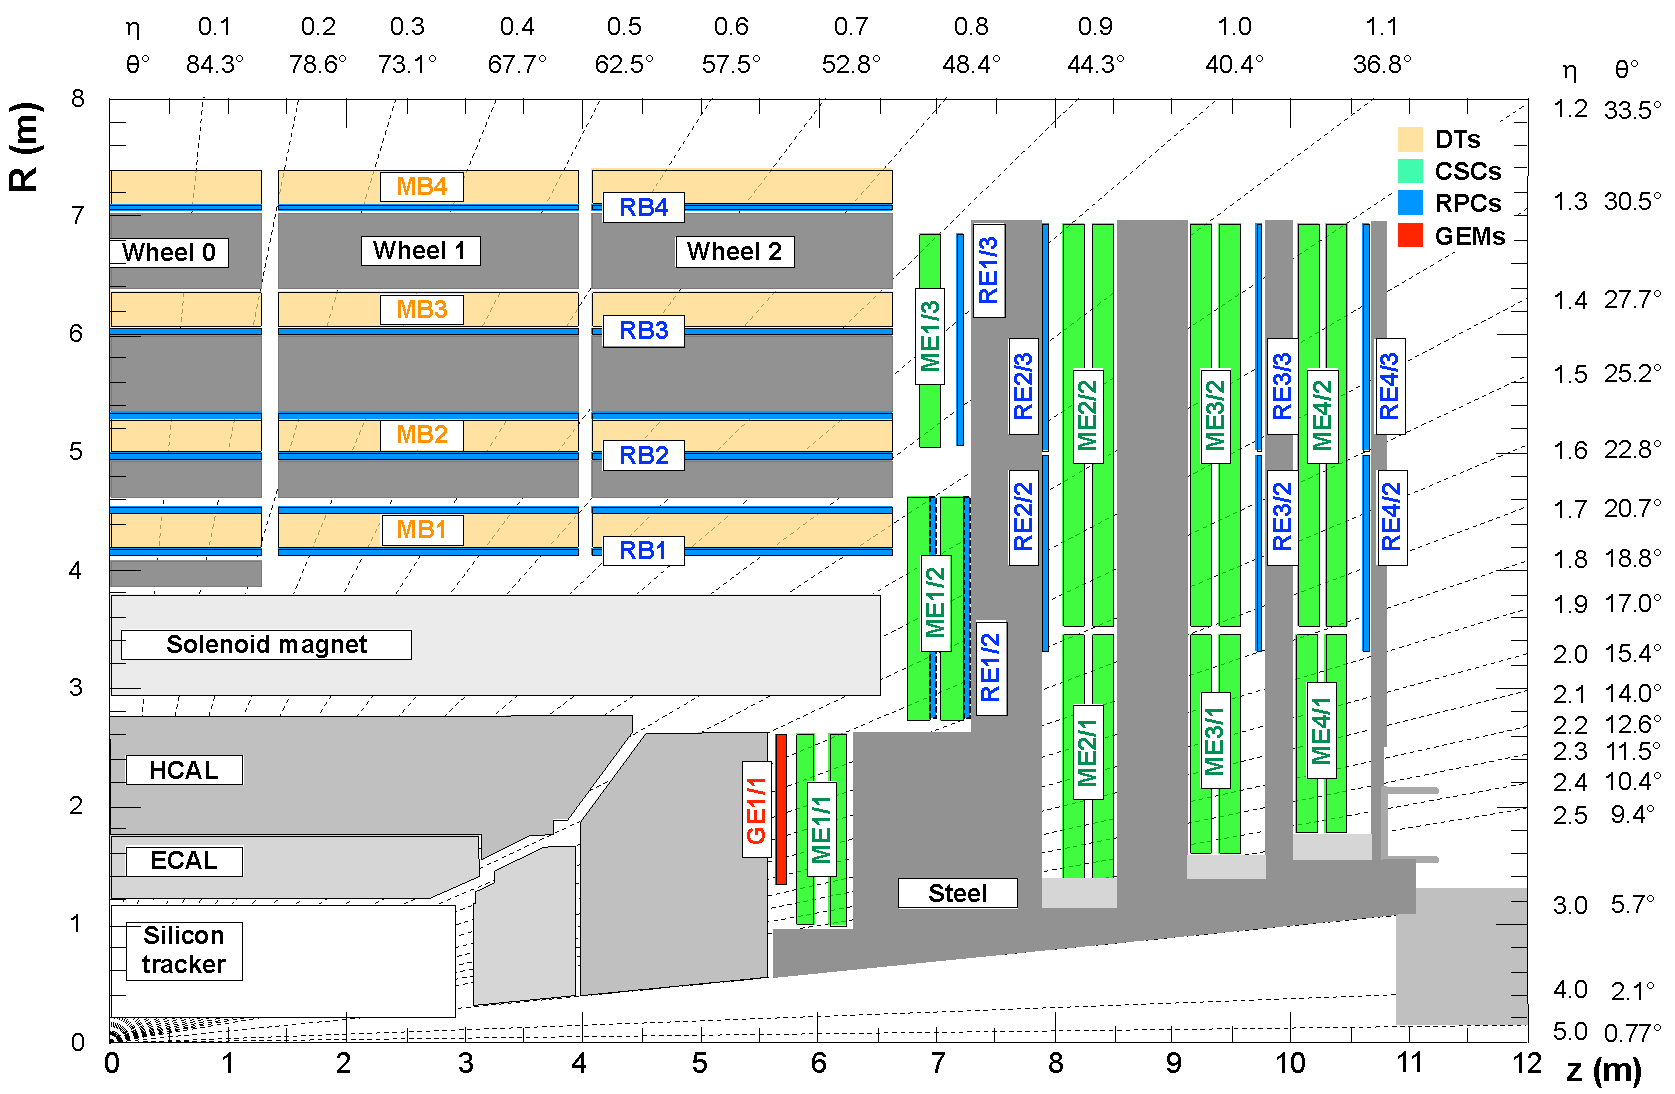
\includegraphics[width=0.99\linewidth]{figures/cms_upg_o_g_b_ni_ge11_r_grid_130919.pdf}
                \caption{Quarter-view of the CMS cross section. Detectors in the muon system are highlighted: DT -- orange, CSC -- green, RPC -- blue and future GE1/1 -- red.}
                \label{fig:CMS_muon_system}
        \end{center}
\end{figure}

The muon trigger is a tracking trigger that determines the momentum of muons using hits (position and angular measurements) in the muon system chambers situated in the magnetic field of the CMS detector. In this paper we describe several major improvements and upgrades to the muons system and their effect on the muon trigger performance. The focus of the muon trigger upgrade is to improve its rate reduction capability without significantly affecting the efficiency. We overview implementation of the muon trigger in endcaps in Section~\ref{sec:endcap_trigger}.

Installation of the outermost ring of CSCs in the fourth disk of each endcap (ME4/2) during 2013-2015 shutdown of the LHC (Long Shutdown 1 or LS1) allows to increase the number of muon hits along its trajectory. Major revision of the electronics for innermost ring of CSCs in the first disk (ME1/1) and unganging strips in the bottom part of these chambers allow to significantly enhance their performance in the trigger and in offline reconstruction. We describe details of the CSC upgrade during LS1 in Section~\ref{sec:csc_upgrade}.

New, robust and sophisticated, ME1/1 local trigger algorithm which is tolerant of the increased pile-up was also developed during LS1. Individual improvements of the upgraded algorithm are studied in details using simulation, and ranked in terms of their importance. The goal is to have improved ME1/1 local trigger algorithm commissioned during the 2015-16 Year-End Technical Stop (YETS), so that the upgraded trigger will be available to operate under high pile-up running conditions in 2016. Overview of the CSC local trigger algorithm is in Section~\ref{sec:csc_algo}. Specifics of the previous and upgraded algorithms implementation in electronics firmware, emulation in CMS software, as well as results of individual improvements are described in three sections:
\begin{enumerate}
\item anode signal processing (see Section~\ref{sec:alct}),
\item cathode signal processing (see Section~\ref{sec:clct}),
\item cathode-anode correlation (see Section~\ref{sec:lct}).
\end{enumerate}

As a part of future upgrade for Phase II of LHC running, the CMS will be equipped with Gas Electron Multiplier (GEM) detectors in the high pseudorapidity region ($1.5 < |\eta| < 2.2$) as shown in Fig.~\ref{fig:CMS_muon_system}. Pairs of triple-GEM chambers will be installed in the currently vacant position in front of the ME1/1 chambers and are dubbed GE1/1. The addition of such chambers allows to measure the bending angle of a track between GE1/1 and ME1/1. Usage of the bending angle at L1 can help to keep the rates down while having the efficiency high. Several implementation possibilities of the combined GEM-CSC local trigger algorithm for the high luminosity run of LHC are investigated in details in~\cite{CMS_DN-14-018}.
\clearpage

\newpage
\tracinginput{sections/sec_endcap_trigger.tex}
%\section{Muon Trigger in Endcaps}
\label{sec:endcap_trigger}

Each CSC can provide up to two local charged track (LCT) segments to the trigger logic per BX. These are formed in the trigger motherboard (TMB) combining cathode (CLCT) and anode (ALCT) segments. Present and improved logics of the algorithm which constructs LCTs are described in Section~\ref{sec:present_algo} and Section~\ref{sec:SLHC_algo}, respectively. The CLCT data contains information on the azimuthal position of the segment ($\phi$), the bend angle, and the pattern of cathode half-strips with hits in a chamber. The ALCT data contains information on the radial position from the beamline of the segment (equivalent to $\eta$), and the pattern of anode wires with hits in a chamber. The timing information from anodes is used to define the time of the combined LCT. There is one TMB per CSC, located in a crate on the periphery of the detector. The TMB sends up to two LCTs over a custom backplane to the muon port card (MPC), which is located in the same peripheral crate. One MPC can receive data from up to 9 TMBs, or equivalently, can receive up to 18 LCTs. The LCTs in a MPC are sorted by rank (see definition in MPC documentation). The best three LCTs are sent over optical fibers to the CSCTF. There are a total of sixty peripheral crates for the CSC system, each with one MPC.

The CSCTF system is partitioned into sectors, each of which corresponds to a $60^{o}$ azimuthal region of an endcap. Twelve ``sector processors'' are required for the entire endcap muon system, six per endcap. Each sector processor is a 9U VME card that is housed in a single crate. Three 1.6 Gb/s optical links from each of five MPCs are received by each sector processor, for a total of 180 optical links for the entire system. The CSCTF sectors are independent, since there is no sharing of data across boundaries of neighboring sectors, leading to slight inefficiencies.

There are several Field Programmable Gate Arrays (FPGAs) on each ``sector processor'', but the main FPGA for the track-finding algorithms is from the Xilinx Virtex-5 family. The conversion of strip and wire positions of each track segment to ($\eta, \phi$) coordinates is accomplished via a set of cascaded SRAM look-up tables (LUTs), each $512K\times16$ bits. These coordinates are then used for track-finding and momentum assignment.

The CSCTF track-finding logic consists of pairwise comparisons of track segments in different detector stations. These test for compatibility in $\phi$ and $\eta$ with a muon emanating from the collision vertex within certain tolerance windows. The comparisons are then analyzed and built into tracks consisting of possibly more than two segments from different stations. Possible duplicate (?ghost?) tracks are canceled. The track-finding logic has the ability to accept segments in different assigned bunch crossings by analyzing across a sliding time window of programmable length (nominally 2 BX) every bunch crossing. Duplicate tracks found on consecutive bunch crossings are canceled. The bunch crossing of a track is given by the second arriving track segment.

The $p_T$ of a muon candidate is calculated by using a large LUT implemented in SRAM. Information such as the track type, track $\eta$, the segment $\phi$ differences between a maximum of 3 stations, and the segment bend angle in the first measurement station are used to calculate the LUT address.

In addition to identifying muons from proton collisions, the CSCTF processors also simultaneously identifies any beam halo muons for monitoring and veto purposes by looking for trajectories approximately parallel to the beam line.

Each CSCTF sends up to three muon candidates per bunch crossing over a custom backplane to a muon sorter (MS). The MS then sorts the candidates by momentum and quality and selects the best 4 for the GMT. The CSCTF data are also sent to a DAQ card with SLINK interface which puts the trigger data into the event record.

\clearpage

\newpage
\tracinginput{sections/sec_endcap_upgrade.tex}
%\section{Endcap Muon System Upgrade}
\label{sec:csc_upgrade}

All CSCs in ME4/2 rings have been installed during LS1. This results in four measurement stations for muons in the region $1.25 < |\eta| < 1.8$ providing additional redundancy in a high rate environment. This redundancy is especially important for future upgraded Global Muon Trigger (GMT) algorithms. For the CSC Track Finder (TF) additional measurement in this region will increase the efficiency and improve the rate reduction since it will be more likely to have 3 or more hits used in the $p_T$ assignment logic. No additional hardware or reconfiguration of the present muon trigger was required after this upgrade. The muon sector receiver boards for the fourth disk already were in place and the present CSCTF already had logic to process trigger data from these chambers.

Electronics for the CSCs have been also under major revision during LS1. All CSCs in ME1/1 rings received new digital cathode front-end boards (DCFEB) as well as new optical trigger motherboards (OTMB) and optical data acquisition motherboars (ODMB) as schematically shown in Fig.~\ref{fig:me11_upgrade_overview}. The new electronics will significantly enhance ME1/1 performance in the trigger and in the offline reconstruction providing a key sagitta measurement for the muon L1 trigger in the region $1.6 < |\eta| < 2.4$. The recovered old electronic boards were used to instrument the newly installed ME4/2 chambers.

The strips of the ME1/1 chambers are split into two regions at $|\eta| = 2.1$ (see details on mechanical layout and signal readout of the ME1/1 chambers in Appendix~\ref{app:me11}). The bottom region ($2.1 < |\eta| < 2.4$) previously had 48 strips triple-ganged to 16 channels in the electronics for both the trigger and the readout, making hit recognition ambiguous. The ambiguity can be mitigated using measurements from the outer stations. However, the $p_T$ resolution using only the outer stations is quite coarse, leading to a significantly increased single muon trigger rate in the forward region $2.1<|\eta|<2.4$. As a result, this region generated a single muon trigger rate comparable to that of the entire region $|\eta| < 2.1$. With the new seven DCFEBs per chamber, this triple-ganging is removed, leading to improved triggering performance in the forward region which allows to maintain highly efficient muon trigger coverage up to $|\eta| = 2.4$.

\begin{figure}[b]
        \begin{center}
                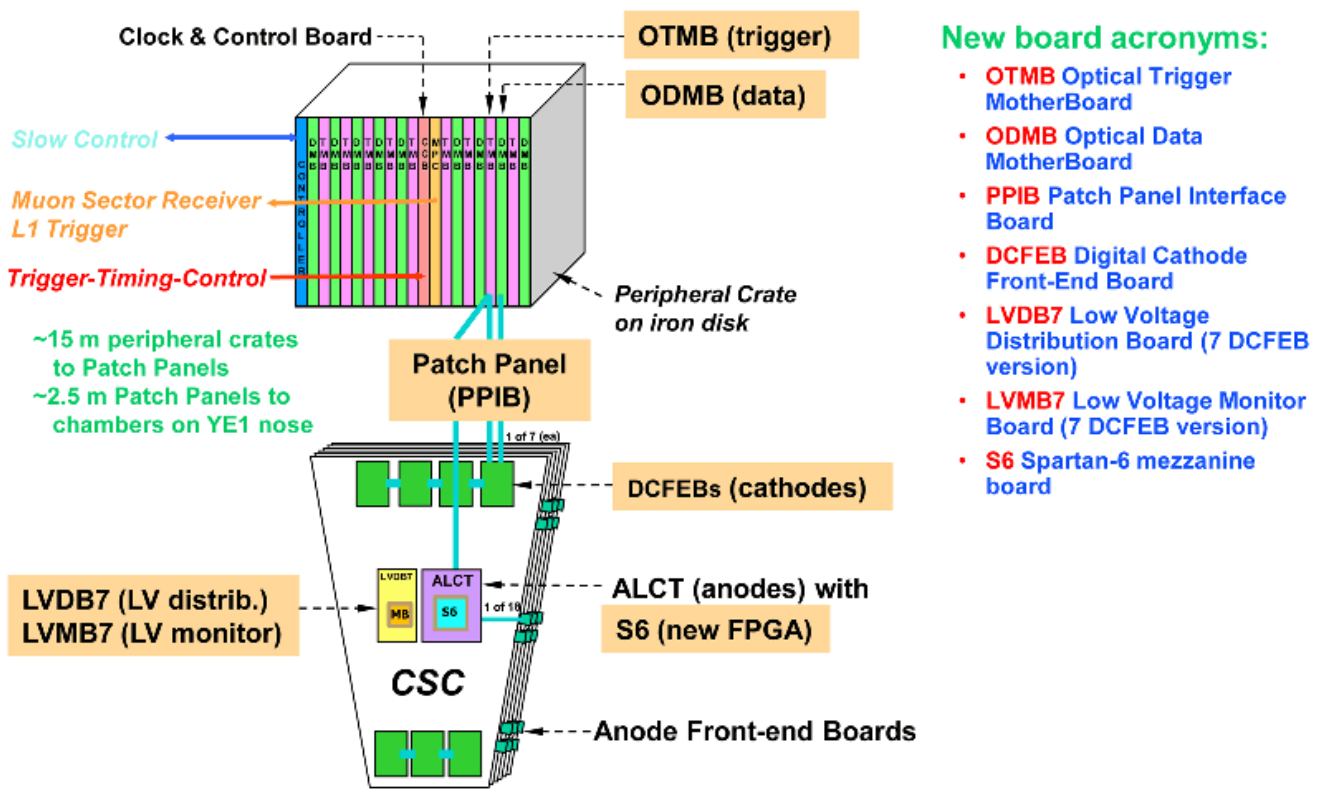
\includegraphics[width=0.85\linewidth]{figures/ME11_upgrade_overview.png}
                \caption{Schematic overview of the ME1/1 electronics upgrade after LS1.}
                \label{fig:me11_upgrade_overview}
        \end{center}
\end{figure}
\clearpage

\newpage
\tracinginput{sections/sec_algorithm.tex}
%\section{Overview of the CSC Local Trigger Algorithms}
\label{sec:csc_algo}

An improved ME1/1 local trigger algorithm to perform sophisticated background rejection is developed for operation under high pile-up running conditions.

\subsection{Results of Improvements in the ME1/1 Local Trigger Algorithm}
\label{sec:SLHC_algo_results}

This chapter presents results of the study of effects of individual improvements described in Sec.~\ref{sec:SLHC_algo} on the ALCT, CLCT, and LCT reconstruction efficiencies.

The study is performed with Monte Carlo simulation of double muon events mixed with PU400 events, where the simulation includes GEN, SIM, DIGI, L1 steps.

Three are three baseline configurations of L1 step used in this study:
\begin{itemize}
	\item Baseline 1: SLHC configuration, where the maximum set of improvements is turned off bringing it to 2007 configuration as close as possible. 
	There are only two differences between Baseline 1 and 2007 configurations: separate treatments of ME1/1a and ME1/1b, and unganging cathode strips in ME1/1a;
	\item Baseline 2: Baseline 1 configuration with all improvements on the ALCT and CLCT processors level turned on;
	\item Baseline SLHC: best CSC4 configuration itself.
\end{itemize}

All algorithm improvements divided into three groups and studied with improvements in the given group turned on one by one on top of each other
\begin{itemize}
	\item ALCT processor level
	\item CLCT processor level
	\item TMB level
\end{itemize}

In the first two groups the L1 step configuration gradually changes from Baseline 1 to Baseline 2 configuration, in the last one --- from Baseline 2 to SLHC configuration.
\clearpage

\newpage
\tracinginput{sections/sec_algorithm_alct.tex}
%\section{Anode Signal Processing}
\label{sec:alct}

\subsection{ALCT Algorithm}
\label{subsec:alct_algo}

Anode wires in CSC are hardwired together at the readout end in groups of 10-15 wires in order to reduce channel count. The anode wire group (WG) signals are fed into the anode front-end boards (AFEBs), each of which contains a single 16-channel amplifier/constant-fraction discriminator chip. The output signals from the AFEBs are sent into the on-chamber ALCT board, which handles triggering and readout of the CSC anode information. Due to the various sizes of CSCs, there are 3 types of ALCT boards, handling 288, 384, and 672 WG channels.

On the ALCT boards, the signals from each AFEB are first delayed by a programmable amount of time in order to perform an average time alignment of the anode signals across the chamber as well as chamber-to-chamber at a sub-bunch crossing level to about 2.2 ns precision. After the AFEB signals are received and time-aligned, then they are latched with bunch crossing frequency and fed to a FPGA (Xilinx Virtex family) mounted on a mezzanine card above the ALCT main board for pattern-finding and readout functions.

The algorithm used in the ALCT FPGA for determining muon segment position and bunch crossing is illustrated below. Since the drift time can be longer than 50 ns, the hits are first stretched by 'one-shots' to 6 BX (150 ns) length. Then, a multi-layer coincidence technique in the ALCT pattern circuitry is used to identify the bunch crossing. For each spatial pattern of anode hits, a low coincidence level, typically 2 or more layers, is used to establish timing, whereas a higher coincidence level, typically 4 layers, is used to establish the existence of a muon track. The general idea of a spatial pattern of CSC wire group hits is illustrated below in Fig.\ref{fig:anode_wire_group_hits}.

\begin{figure}[tbh]
        \begin{center}
                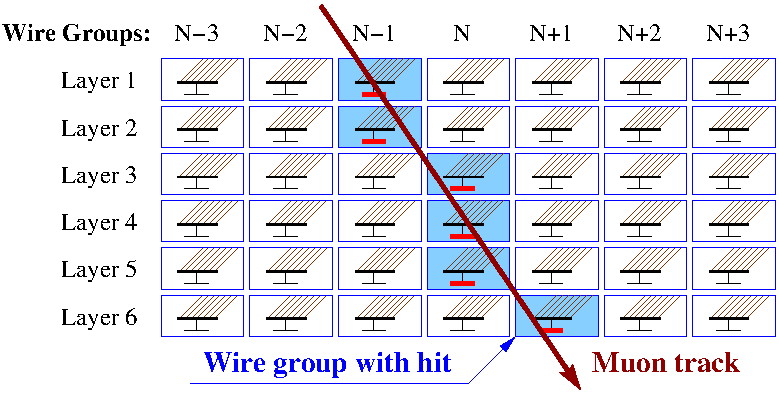
\includegraphics[width=0.6\linewidth]{figures/anode_wire_group_hits.pdf}
                \caption{Illustration of CSC anode wire groups with hits from muon track}
                \label{fig:anode_wire_group_hits}
        \end{center}
\end{figure}

while the general idea of the time stretching of hits, and pretrigger followed by a pattern trigger is shown in Fig.\ref{fig:anode_stretched_hits} (using an example in which one hit is actually missing due to some type of inefficiency).

\begin{figure}[tbh]
        \begin{center}
                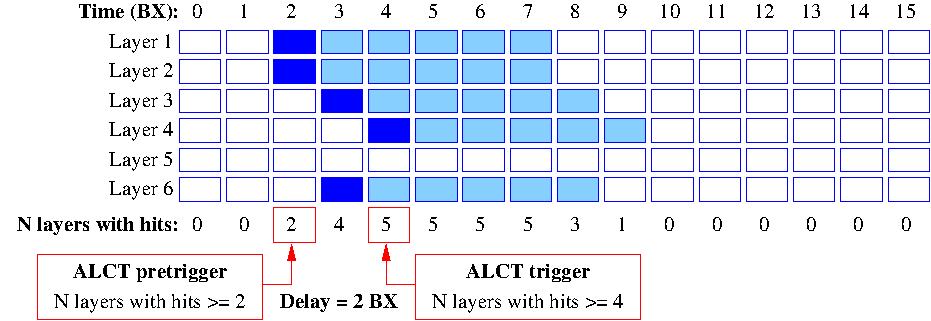
\includegraphics{figures/anode_stretched_hits.pdf}
                \caption{Illustration of anode hits time stretching (6BX) as well as determination of ALCT pretrigger and trigger.}
                \label{fig:anode_stretched_hits}
        \end{center}
\end{figure}

Each pattern detector can detect a programmable "collision" pattern as well as a fixed "accelerator" pattern. The input data for the collision pattern detector are selected as shown below:

\begin{center}
\begin{verbatim}
...n-2 n-1 n...........Layer 1
.......n-1 n...........Layer 2
...........n...........Layer 3
...........n n+1.......Layer 4
...........n n+1 n+2...Layer 5
...........n n+1 n+2...Layer 6
\end{verbatim}
\end{center}

where n in this diagram is the key wire group number, which this particular pattern detector is searching the patterns for. The programming of the programmable collision pattern is implemented as a simple masking-out of the bits that we do not want to include in the pattern. The accelerator pattern is a vertical pattern of 6 layers all with strip n only.

Each ALCT candidate is assigned a quality equal to number of layers with hits minus 3 and passes through a ghost cancellation procedure: it is cancelled if there is another ALCT candidate at the same bunch crossing in the previous wirewith the same or better quality or in the next wire with better quality, or if there is ALCT candidate up to 4 bunch crossing clocks earlier with any quality.

In each bunch crossing two ALCTs with highest quality are sent to the TMB (Trigger MotherBoard), which requires a coincidence between anode and cathode trigger information. In the case of a Level-1 Accept signal from the Global Trigger (distributed via the TTC system to the CCB in each peripheral crate), ALCT data are sequentially transmitted to the Trigger Mother Board and hence to the DAQ Motherboard. These data frames include a few words of ALCT trigger data and a much larger amount of ALCT raw hit data consisting of a time sequence of raw CSC anode wire-group hits that have been stored at the 40 MHz bunch crossing frequence by the ALCT2001. Typically 8 to 16 bunch crossings are read out for each wire group. FIFO data can also be read out much more slowly through VME access via the TMB board using a JTAG electrical interface to the ALCT, if necessary.

For self-monitoring and also for powering and controlling the AFEB cards, the ALCT contains a Slow Control section that supplies power to the AFEBs, controls AFEB thresholds, provides and controls the amplitude of test pulses to the AFEBs, and reads back power supply voltages and currents, as well as on-board temperature. 

\subsection{Improvement of the ALCT Algorithm}
\label{subsec:alct_improvements}

It should be possible to improve the efficiency, rate and timing precision of ALCT stubs by, e.g.
\begin{itemize}
    \item tuning of the ghost cancellation logic (ALCTs in neighboring wiregroups, see "alctGhostCancellationBxDepth" and "alctGhostCancellationSideQuality" parameters in Sec.~\ref{sec:ALCT_conf}) and removing pre-trigger deadtime (see "alctPretrigDeadtime" parameter in Sec.~\ref{sec:ALCT_conf});
    \item using more narrow ALCT pattern in ring 1 chambers (see "alctNarrowMaskForR1" parameter in Sec.~\ref{sec:ALCT_conf});
    \item using more precise algorithm (e.g., running median or truncated average) for BX assignment (see "alctUseCorrectedBx"  parameter in Sec.~\ref{sec:ALCT_conf}).
\end{itemize}

However, here we would only like to focus on how the ALCT stubs would be used by TMB.

ALCTs are reconstructed from the signals in layers of anode wires which are ganged into wiregroups and are continuously covering the whole ME1/1 chamber. Most of the wiregroups can only physically cross only strips either in ME1/1a or only in ME1/1b. A complication specific to ME1/1 is that wires here are not perpendicular to strips, but are slanted at 29 degrees from the straight angle. Thus, some wiregroups are crossing the border between ME1/1a and ME1/1b. If signal is detercted in such a wiregroup, there is an ambiguity about which part of ME1/1 it might belong to.

For the ALCTs received by TMB we propose to split the incoming stubs into two parts, ME1/1a and ME1/1b, that would be used further for LCT matching separately in ME1/1a and ME1/1b. 




\subsection{Emulation of ALCT Algorithm}
\label{subsec:alct_emulation}

ALCT processing includes the following five steps:

\begin{itemize}
    \item Pulse extension;
    \item Pretrigger;
    \item Trigger;
    \item Ghost cancellation;
    \item ALCT construction.
\end{itemize}

\subsubsection{Pulse Extension}

Sofware emulation provides information about all wire signals in DAQ readout window (16 BXs). A search for these signals is performed in a loop over all wire groups, all layers, and all 16 BXs; found signals are stretched over 6 BXs (see Fig.~\ref{fig:alct_pulse_extension}).

\begin{figure}[tbh]
        \begin{center}
                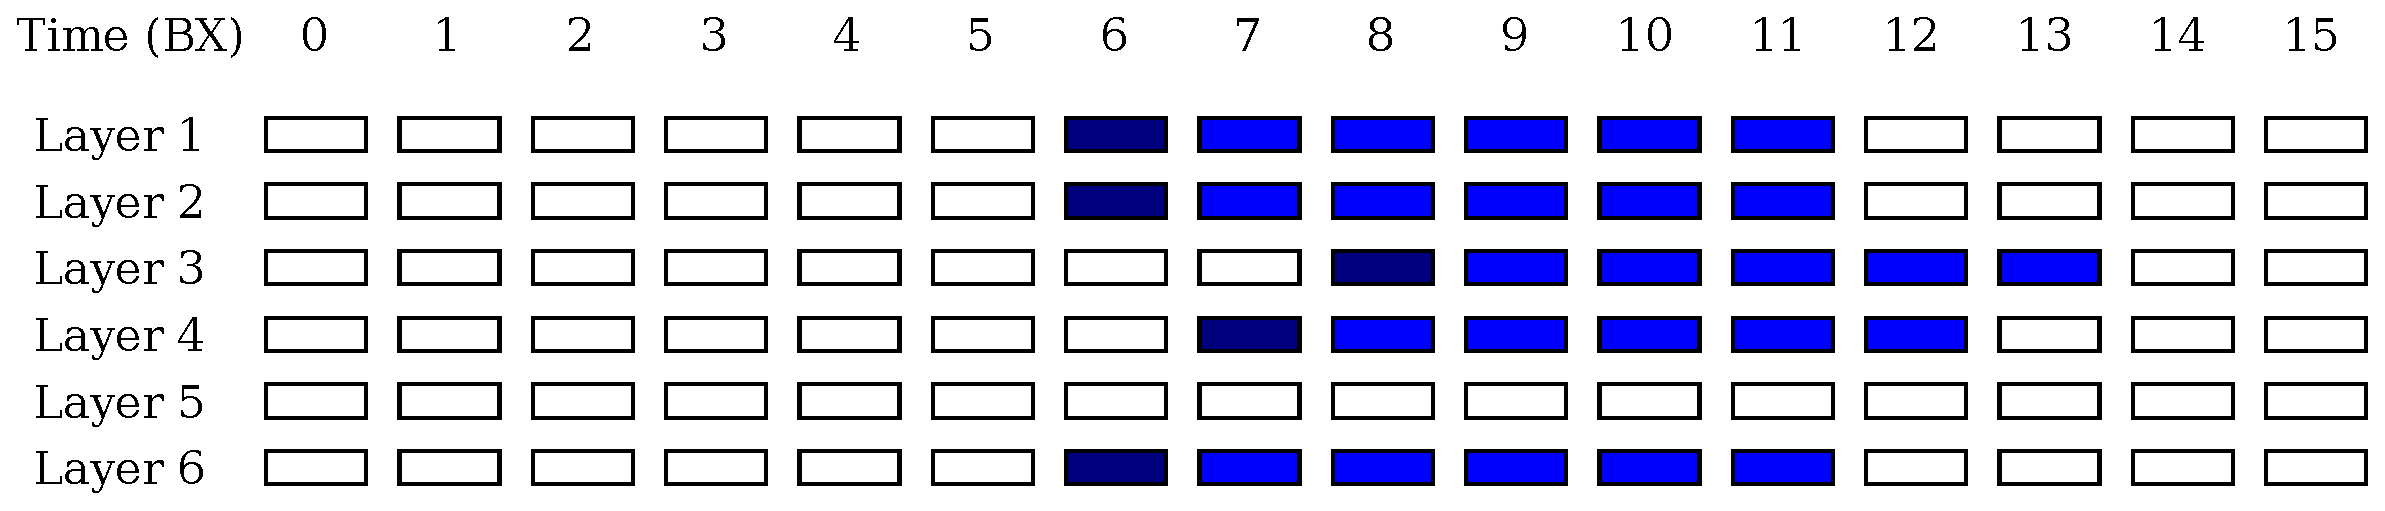
\includegraphics[width=0.9\linewidth]{figures/stretched_hits_alct.pdf}
                \caption{Illustration of ALCT pulse extension for one specific wire group.}
                \label{fig:alct_pulse_extension}
        \end{center}
\end{figure}

\subsubsection{Pretrigger}

After all available wire signals are stretched, a search for ALCT pretriggers is performed in all wire groups and all BXs. For any given wire group and BX, we count the number of layers with hits within the pattern mask shown on Fig.~\ref{fig:alct_pretrigger}, and if this number is greater than or equal to three, then we say that a pretrigger occured in this wire group and BX. The search for next ALCT pretrigger starts 6 BXs later.

\begin{figure}[tbh]
        \begin{center}
                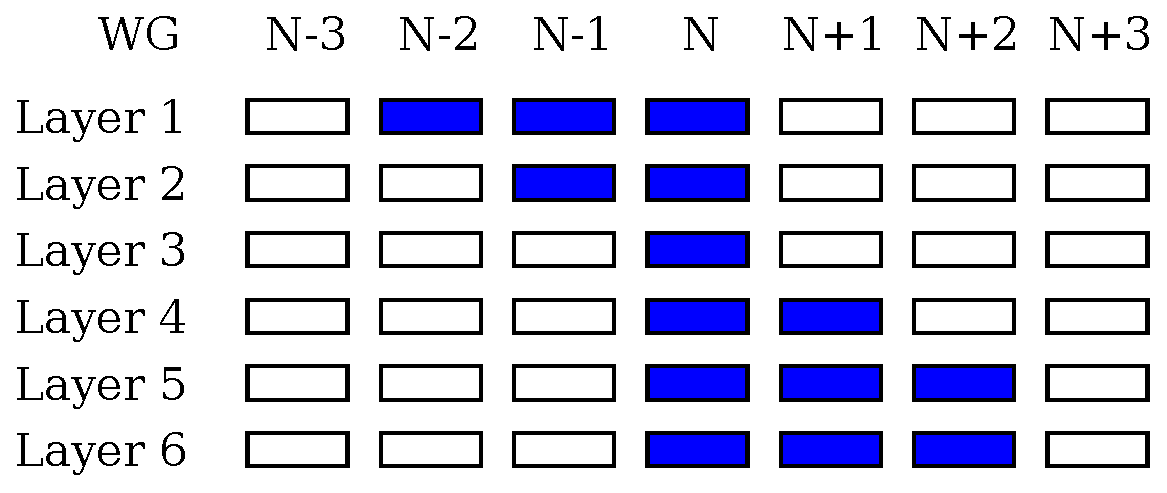
\includegraphics[width=0.45\linewidth]{figures/alct_pretrigger.pdf}
                \caption{ALCT pattern mask for pretriggering and triggering.}
                \label{fig:alct_pretrigger}
        \end{center}
\end{figure}

\subsubsection{Trigger}

After all ALCT pretriggers are found, for each pretrigger in BX = B we check for a trigger in BX = B+2. For any given wire group and BX = B+2, we count the number of layers with hits within the same pattern mask used for pretriggering, and if this number is greater than or equal to four, we say that a pretrigger occured in this wire group and BX, and assign it a quality Q = number of layers with hits-3. If in some wire group more than one trigger occured, we report only the one with the highest quality. If there are two triggers with the same quality, report the earlier one.

\subsubsection{Ghost Cancellation}

Not all triggers found in the previous step are used to construct ALCTs: before that all of them pass through so called ghost cancellation procedure.

A trigger in wire group = N and BX = B is cancelled if there is a trigger in wire group = N-1:
\begin{itemize}
    \item either in the same BX = B and with better or equal quality;
    \item or to 4 BXs earlier, with any quality.
\end{itemize}

In addition, a trigger in wire group = N and BX = B is cancelled if there is a trigger in wire group = N+1:
\begin{itemize}
    \item either in the same BX = B and with better quality;
    \item or to 4 BXs earlier, with any quality.
\end{itemize}

\subsubsection{ALCT Construction}

Construct ALCTs from triggers survived after the ghost cancellation procedure: encode quality, WG, BX (defined by pretrigger BX). In every BX choose best two ALCTs: two ALCTs with the highest quality. If we need to choose one ALCT from two ALCTs with the same quality: choose the one with larger wire group.


\subsection{Sofware Emulation of ALCT Level Improvements}

\subsubsection{Tuning of Ghost Cancellation Procedure}

\textcolor{red}{Current} ghost cancellation:
\begin{itemize}
    \item Loop over wire groups:
    \begin{itemize}
        \item Consider WG = N
        \item Cancel trigger in this wire group if there is trigger in WG = N-1 and:
        \begin{itemize}
            \item with the same BX and with \textcolor{red}{better or equal} quality
            \item up to \textcolor{red}{4} BXs earlier, with \textcolor{red}{any} quality
        \end{itemize}
        \item Cancel trigger in this wire group if there is trigger in WG = N+1 and:
        \begin{itemize}
            \item with the same BX and with \textcolor{red}{better} quality
            \item up to \textcolor{red}{4} BXs earlier, with \textcolor{red}{any} quality
        \end{itemize}
    \end{itemize}
\end{itemize}
\textcolor{blue}{New} ghost cancellation:
\begin{itemize}
    \item Loop over wire groups:
    \begin{itemize}
        \item Consider WG = N
        \item Cancel trigger in this wire group if there is trigger in WG = N-1 and:
        \begin{itemize}
            \item with the same BX and with \textcolor{blue}{better} quality
            \item up to \textcolor{blue}{1} BX earlier, with \textcolor{blue}{better} quality
        \end{itemize}
        \item Cancel trigger in this wire group if there is trigger in WG = N+1 and:
        \begin{itemize}
            \item with the same BX and with \textcolor{blue}{better or equal} quality
            \item up to \textcolor{blue}{1} BX earlier, with \textcolor{blue}{better and equal} quality
        \end{itemize}
    \end{itemize}
\end{itemize}

The following modifications in configuration are related to this improvement:
\begin{itemize}
    \item alctGhostCancellationBxDepth: 4BX to 1BX
    \item alctGhostCancellationSideQuality: False to True
\end{itemize}

\subsubsection{Narrow ALCT Pattern Mask}

Use more narrow ALCT pattern mask for stations in Ring 1 (see Fig.~\ref{fig:narrow_alct_pattern_mask}).

\begin{figure}[tbh]
        \begin{center}
                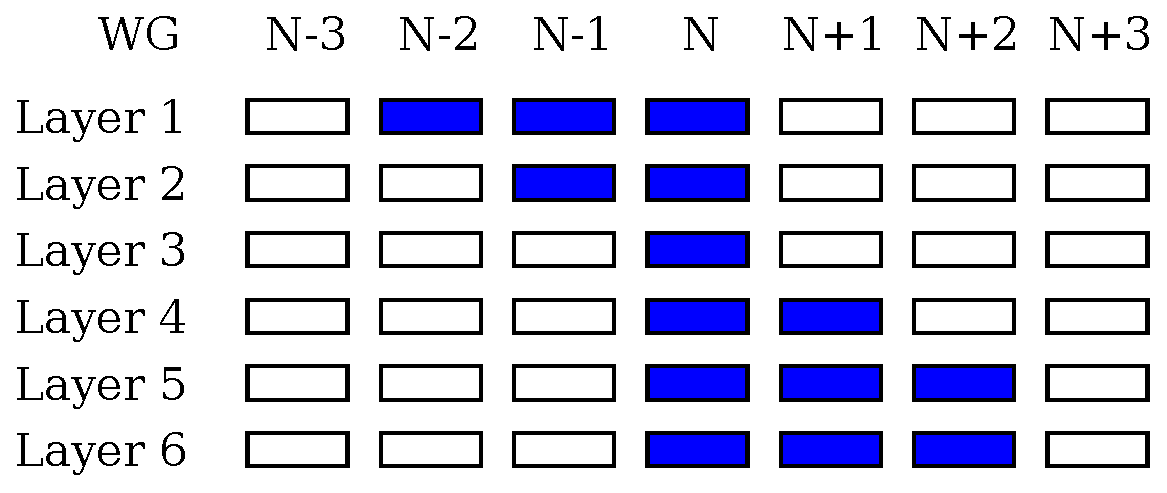
\includegraphics[width=0.49\linewidth]{figures/alct_pretrigger.pdf}\\
                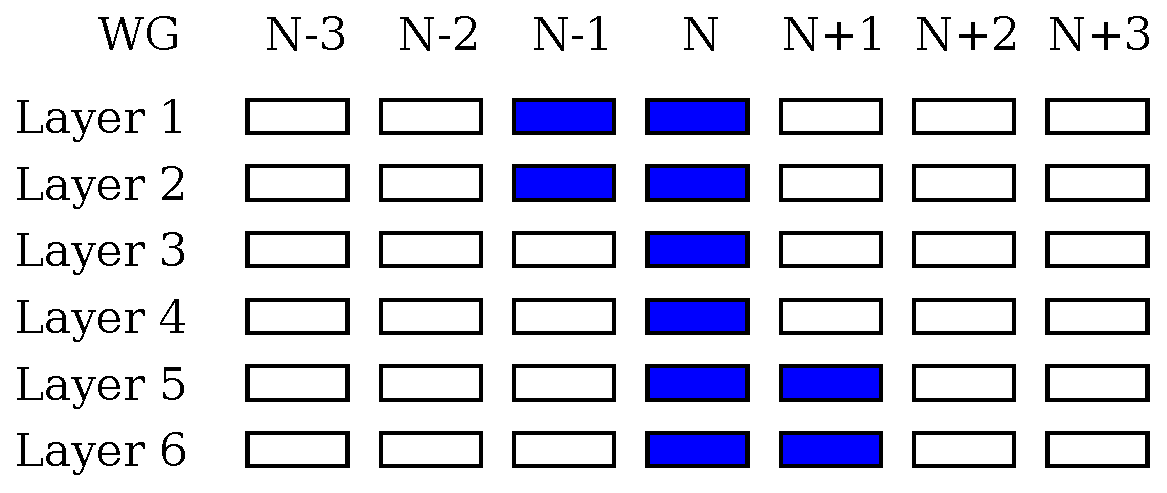
\includegraphics[width=0.49\linewidth]{figures/alct_pretrigger_r1.pdf}
                \caption{Top: default ALCT pattern mask, bottom: narrow ALCT pattern mask.}
                \label{fig:narrow_alct_pattern_mask}
        \end{center}
\end{figure}

The following modifications in configuration are related to this improvement:
\begin{itemize}
    \item alctNarrowMaskForR1: False to True
\end{itemize}

\subsubsection{Reduced ALCT Dead Time}

Currently, if there is pretrigger in BX = B (see Fig.~\ref{fig:alct_deadtime}):
\begin{itemize}
    \item Check for trigger in BX = B + drift time = B+2
    \item Search for next pretrigger starting from BX = B + drift time + extra deadtime = B+6
\end{itemize}

Suggested improvement: decrease extra deadtime from 4 BX to 0 BX.

\begin{figure}[tbh]
        \begin{center}
                \includegraphics[width=0.98\linewidth]{figures/stretched_hits_alct_deadtime.pdf}
                \caption{Top: Dead Time between ALCT pretriggers.}
                \label{fig:alct_deadtime}
        \end{center}
\end{figure}

The following modifications in configuration are related to this improvement:
\begin{itemize}
    \item alctPretrigDeadtime: 4BX to 0BX
\end{itemize}


\subsection{Results of Improvements of the ALCT Processing}

Improvements on the level of ALCT processor are related to the following configuration parameters (see Sec.~\ref{sec:ALCT_conf}):
\begin{itemize}
	\item alctGhostCancellationBxDepth: 4BX to 1BX;
	\item alctGhostCancellationSideQuality: False to True;
	\item alctNarrowMaskForR1: False to True;
	\item alctPretrigDeadtime: 4BX to 0BX.
\end{itemize}

Fig.~\ref{fig:ALCT_improvements_ALCT_recoEff} shows reconstruction efficiency of a good ALCT in ME1/1 station versus pseudorapidity of the simulated muon for different L1 configurations. The good ALCT is defined as ALCT:
\begin{itemize}
	\item read out in the window of 3BX around the central BX (BX6);
	\item reconstructed within 2 anode wire groups from the key wire group.
	\item has hits at least on four layers
\end{itemize}

The major improvement in ALCT reconstruction efficiency comes from the changes in ALCT ghost cancellation procedure.

\begin{figure}[p]
\includegraphics[width=0.98\textwidth]{figures/ALCT_improvements_ALCT_recoEff.png}
\includegraphics[width=0.98\textwidth]{figures/ALCT_improvements_ALCT_recoEff_PU50.png}
\caption{ALCT reconstruction efficiency in ME1/1 station for PU140 (top) and PU50 (bottom). Muons with transverse momentum $10$~GeV$<p_T<50$~ GeV are used in the analysis.}
\label{fig:ALCT_improvements_ALCT_recoEff}
\end{figure}
\clearpage

\newpage
\tracinginput{sections/sec_algorithm_clct.tex}
%\section{Cathode Signal Processing}
\label{sec:clct}

\subsection{CLCT Algorithm}
\label{subsec:clct_algo}

[We need a good picture illustrating CLCT processing process like in the case of ALCT one]

A muon passing through a CSC chamber will produce distinctive patterns of half-strip
hits in the six-layer endcap muon CSC chambers. By identifying these patterns, the CSC Local
Trigger provides high rejection power against backgrounds. The largest background source,
neutron-induced gamma ray conversions, are generally low in energy, and produce mostly single-
layer or short multi-layer hits. Other backgrounds, such as low-momentum muons or punch-
through particles often do not point well enough to the primary interaction region to be considered
high-momentum muon candidates.

\begin{figure}[tbh]
        \begin{center}
                \includegraphics[width=0.73\linewidth]{figures/CLCT_block_diagram.png}
                \caption{CLCT block diagram}
                \label{fig:clct_block_diagram}
        \end{center}
\end{figure}

[Technical description from TMB manual below]

For each of 160 key half-strips consider the 42 neighboring half-strips (i.e. on key 5 use the following half-strips):

\begin{figure}[tbh]
        \begin{center}
                \includegraphics[width=0.48\linewidth]{figures/160_key_half_strips.png}
                \caption{160 key half-strips}
                \label{fig:160_key_half_strips}
        \end{center}
\end{figure}

For each of 160 key half-strips, count layers with hits matching the 9 pattern templates:

\begin{figure}[tbh]
        \begin{center}
                \includegraphics[width=0.98\linewidth]{figures/CLCT_patterns.png}
                \caption{CLCT patterns}
                \label{fig:clct_patterns}
        \end{center}
\end{figure}

Pattern ID=1 is a layer-OR trigger, Pattern ID=0 is no-pattern-found. Result for each of 160 keys is a list of 9 pattern-ID numbers (pid) [2 to A] and corresponding
number of layers [0 to 6] with matching hits (nhits). Find the best 1-of-9 pattern ID numbers for each key by comparing nhits. Ignore bend direction: left and right bends have equal priority (bit 0 of pid implies bend direction).
If two pattern IDs have the same nhits, take the higher pattern ID. A key with no matching hits, would always return pid=A and nhits=0.
Pre-trigger if any 1-of-160 keys have nhits $\geq$ hit\_thresh\_pretrig and pid $\geq$ pid\_thresh\_pretrig.

Construct 7-bit pattern quality pat[7:0] for sorting where pat[7:5]=nhits[2:0], pat[4:0]=pid[3:0]. Ignore the bend direction bit (pid[0]), left and right bends have equal priority. 
Store pat[7:0] for 160 keys for use later to find 2nd CLCT.
Find the best key out 1-of-160 keys by sorting on the 6-bit number pat[7:1]. Store 1st CLCT info: key, pattern ID, and number of hits.
For empty events, key=0, pid=A and nhits=0. If clct\_blanking=1, then key=pid=hits=0.

Mark keys near 1st CLCT as busy from 1st key-nspan to 1st key+pspan.
If clct\_sep\_src=1, pspan and nspan are set equal to clct\_sep\_vme, typically 10 half-strips.
If clct\_sep\_src=0, pspan and nspan are read from RAM and depend on the pattern ID number, this allows two less bending tracks to be closer than more bending tracks.

Find the best key out of 1-of-160 keys by sorting on the 6-bit number pat[7:1]: skip busy keys, if two keys have the same pat[7:1] take the lower key.
Store the same information for the 2nd CLCT as for the 1st one.

Wait for CSC drifting (drift delay of 2BXs) and perform matching to ALCTs.


\subsection{Separation of the CLCTs in ME1/1a and ME1/1b}

In the old TMB f/w, the 16 ganged strip channels from ME1/1a are appended to the 64 ME1/1b strip channels and the reconstruction of CLCTs is performed as if it's a single regular chamber with 80 channels (is there any treatment of the boundary, so that ME1/1a strips are not combined with ME1/1b strips?). The two rather separate and distinctive areas combined and treated like one uniform unit with the maximum of two CLCT stubs on the output.

With unganged ME1/1a and higher pile-up such a simple approach becomes increasingly unnatural and ineffective. The ME1/1a would have x3 more channels now, so it would deserve to be treated like a separate chamber even more. And chances to get multiple stubs are increasing with higher luminosity, especially so in ME1/1a. With multiple stubs, the stubs in ME1/1a would start directly competing with those in ME1/1b.

With a larger size FPGA, it would be beneficial to treat ME1/1a and ME1/1b as two separate chambers for the purpose of CLCT reconstruction, with each area having their own limit on the maximum of 2 CLCTs. Thus, the whole ME1/1 would be able to have maximum 4 CLCTs available for matching with ALCTs. It's important to keep more 2D stubs available so that at the stage of matching we can reduce the number of stubs following some better tuned criteria.

Finally, in the case if we would allow to read out the 2D CLCT stubs without an ALCT match, and we cannot read out more then 2 of them per BX per ME1/1, we can device a selection criteria when comparing stubs from ME1/1a and ME1/1b as follows: e.g., if quality of an ME1/1b stub is the same or less by one then that of an ME1/1a stub, prefer the ME1/1b one. 

\subsection{Localization of the TMB Dead Time}

 The main source of the old TMB inefficiency in high pile-up is the dead time which happens for the whole ME1/1 chamber after there was a triggering CLCT. The TMB's state-machine freezes whole TMB for several BXs after a CLCT trigger while number of coincidence layers stays over the trigger threshold. If anywhere in a chamber there was an CLCT from PU a few BX earlier before a signal muon, it would be impossible to trigger on the signal.

While it's clear that with the comparator information which we recieve in TMB, it's not really possible to distinguish close in time signals in the same strip, there seem to be no apparent reason, other then the complexity of the algorithm, for this dead time to be present in strips that had no trigger.

Thus, the algorithm approach to deal with this issue for the upgrade could be as follows:
\begin{itemize}
    \item when a CLCT trigger happens, mark as busy only those strips within either a fixed dead time zone around CLCT (8 half-strips, see "useDeadTimeZoning" parameter in Sec.~\ref{sec:CLCT_conf}) or within the dead time zone, the width of which depends on the CLCT pattern (from 11 half-strips for the most bent patterns to 3 half-strips for the straightest one, see "useDynamicStateMachineZone" parameter in Sec.~\ref{sec:CLCT_conf}), and also mark the signal half-strip that specifies the triggered CLCT
    \item during the following bunch-crossings, check if the number of coincidence layers drops under the trigger threshold for the signal half-strip
    \begin{itemize}
	\item if it does, remove the "busy" mark from the corresponding strips 
    \end{itemize}
    \item if strips are marked as busy in a BX, they are excluded from pattern recognition 
\end{itemize}

\subsection{Restriction on the CLCT Pattern Bend}

The current set of CLCT patterns (see details in Sec.~\cite{subsec:clct_algo}) is largely geared towards low pt tracks. For tracks with pt>10, only the straighest and the next one bent patterns are significant. The restriction on allowed pattern bending would significantly help with many issues including multiplicity \& rate, ghosting, dead-time and corresponding loss of the efficiency (see "clctPidThreshPretrig" parameter in Sec.~\ref{sec:CLCT_conf}). Positive effect of it would increase with increasing luminosity. However, it would also somewhat reduce the efficiency because of not so good pt-threshold resolution from fairly narrow (11cm) CSC chambers, especially for medium to lower pt muons.

Plots on Fig.~\ref{fig:efficiency_vs_pt} show the efficiency vs $p_T$ for a simulated muon track to have a matching reconstructed CLCT stub for different sets of patterns (which defines maximum thresholds for the bend). Note, that adding GEMs could be helpful for improving the the efficiency of the bend restriction.

\begin{figure}[tbh]
        \begin{center}
                \includegraphics[width=0.48\linewidth]{figures/efficiency_vs_pt.png}
                \includegraphics[width=0.48\linewidth]{figures/efficiency_vs_pt_scale.png}
                \caption{Efficiency vs $p_T$. No pile up is included in the simulated sample.}
                \label{fig:efficiency_vs_pt}
        \end{center}
\end{figure}

\subsection{Improvement of the CLCT Timing}

Currently, the BX time of a CLCT stub is defined as the BX of its pretrigger. Or, in other words, it's first BX when at least three layers fit one of the CLCT patterns. Note that an attempt to latch a trigger pattern is performed after the number of BX after the pretrigger defined by the clctDriftDelay parameter (=2BX). And also note that a CLCT pattern during the pretrigger could be different then the one that happen to match during the trigger.

With higher luminosity there are increasingly larger chances for some strips in some of the layers to be hit by earlier background hit. And that has chances to affect the time when a pretrigger might be detected. A more robust solution would be to define stub's time using the times of its strips, where stub's strips are defined as strips that were matched within a CLCT pattern during the trigger. As for a specific procedure, a median time over those strips' times or some sort of a truncated average could be used (see "clctUseCorrectedBx" parameter in Sec.~\ref{sec:CLCT_conf}, analogously for "alctUseCorrectedBx" parameter in Sec.~\ref{sec:ALCT_conf}).

\newpage
\subsection{Software Emulation of CLCT Processing}

CLCT processing includes the following four steps:

\begin{itemize}
    \item Pulse extension;
    \item Pretrigger;
    \item Trigger;
    \item CLCT construction and CLCT dead time.
\end{itemize}

In contrast to ALCT processing, where all steps are independent and performed one after another for all 16 BXs, during CLCT processing last three steps repeated in one global loop over BXs.

\subsubsection{Pulse Extension}

Sofware emulation provides information about all half-strip signals in DAQ readout window (16 BXs). A search for these signals is performed in a loop over all half-strips, all layers, and all 16 BXs; found signals are stretched over 6 BXs (see Fig.~\ref{fig:clct_pulse_extension}).

\begin{figure}[tbh]
        \begin{center}
                \includegraphics[width=0.9\linewidth]{figures/stretched_hits_clct.pdf}
                \caption{Illustration of ALCT pulse extension for one specific half-strip.}
                \label{fig:clct_pulse_extension}
        \end{center}
\end{figure}

\subsubsection{Pretrigger}

After all available half-strip signals are stretched, start a global loop over all BXs from BX = 0 and search for CLCT pretriggers in all half-strips. For any given BX and half-strip, count the number of layers with hits within the patterns shown on Fig.~\ref{fig:clct_pretrigger}, and if this number is greater than or equal to three, then we say that a pretrigger occured in this BX and this half-strip. This pretrigger is only accepted if its pattern id $\geq$ 2. If there were no CLCTs found in some BX = B, proceed to BX = B+1 and continue searching for pretriggers. If there are some CLCTs found in the current BX, proceed to next step.

\begin{figure}[tbh]
        \begin{center}
                \includegraphics[width=0.48\linewidth]{figures/clct_pattern_01.pdf}
                \includegraphics[width=0.48\linewidth]{figures/clct_pattern_10.pdf}\\
                \includegraphics[width=0.48\linewidth]{figures/clct_pattern_02.pdf}
                \includegraphics[width=0.48\linewidth]{figures/clct_pattern_03.pdf}\\
                \includegraphics[width=0.48\linewidth]{figures/clct_pattern_04.pdf}
                \includegraphics[width=0.48\linewidth]{figures/clct_pattern_05.pdf}\\
                \includegraphics[width=0.48\linewidth]{figures/clct_pattern_06.pdf}
                \includegraphics[width=0.48\linewidth]{figures/clct_pattern_07.pdf}\\
                \includegraphics[width=0.48\linewidth]{figures/clct_pattern_08.pdf}
                \includegraphics[width=0.48\linewidth]{figures/clct_pattern_09.pdf}
                \caption{CLCT patterns for pretriggering and triggering.}
                \label{fig:clct_pretrigger}
        \end{center}
\end{figure}

\subsubsection{Trigger}

As soon as a BX = B with CLCT pretrigger(s) is found, search for triggers in BX = B+2. For each half-strip, count the number of layers with hits within the same patterns used for pretriggering, and if this number is greater than or equal to four, we say that a trigger occured in this half-strip and BX, and remember:
\begin{itemize}
    \item pattern id with the highest number of hit layers (if there are two pattern ids with the same number of hit layers, choose smaller pattern id);
    \item number of hit layers in this pattern id.
\end{itemize}

Proceed to next step.

\subsubsection{CLCT Construction and CLCT Dead Time}

In a BX with CLCT triggers, find up to two best triggers to be used in CLCT construction.

Find the best trigger:
\begin{itemize}
    \item Find trigger with the highest number of hit layers;
    \item If there are two triggers with the same number of hit layers: choose the one with higher pattern id;
    \item If there are two triggers with the same number of hit layers and the same pattern id: choose the one with smaller half-strip.
\end{itemize}

Mark zone of 20 half-strips around the best trigger as used and find the second best trigger among not used half-strips.

Construct up to two best CLCTs from found best triggers: encode quality, pattern, bending direction, half-strip, cfeb, BX (defined by pretrigger BX).

After CLCT construction, keep CLCT "dead": continue the loop over all BXs until there is a BX with no triggers. When such a BX is found go back to pretriggering step.


\newpage
\subsection{Sofware Emulation of CLCT Level Improvements}

\subsubsection{Localizing Dead Zone}

\textcolor{red}{Current implementation of dead time}:
\begin{itemize}
    \item After constructing up to two CLCTs, \textcolor{red}{continue the loop over all BXs until there is a BX with no triggers}
    \\...
    \item In the BX with trigger, construct up to two CLCTs from two best triggers \textcolor{red}{in all half-strips}
    
\end{itemize}
\textcolor{blue}{New implementation of dead time}:
\begin{itemize}
    \item After constructing up to two CLCTs, \textcolor{blue}{mark 16 half-strips around half-strips of these CLCTs as busy while number of hit layers in half-strips of these CLCTs $\geq$ 4}
    \item \textcolor{blue}{After trigger in BX = B, keep searching for pretrigger in strating from BX = B+1}
    \\...
    \item In the BX with trigger, construct up to two CLCTs from two best triggers \textcolor{blue}{in half-strips}
    \begin{itemize}
        \item \textcolor{blue}{within 5 half-strips from pretrigger half-strips}
        \item \textcolor{blue}{which are not marked as busy from previous trigger}
    \end{itemize}
\end{itemize}

The following modifications in configuration are related to this improvement:
\begin{itemize}
    \item useDeadTimeZoning: False to True
\end{itemize}

\subsubsection{Dynamic Dead Zone Width}

\textcolor{red}{Fixed dead time zone}:
\begin{itemize}
    \item After constructing up to two CLCTs, mark \textcolor{red}{16} half-strips around half-strips of these CLCTs as busy while number of hit layers in half-strips of these CLCTs $\geq$ 4
\end{itemize}
\textcolor{blue}{Dynamic dead time zone}:
\begin{itemize}
    \item After constructing up to two CLCTs, mark \textcolor{blue}{K(pid)} half-strips around half-strips of these CLCTs as busy while number of hit layers in half-strips of these CLCTs $\geq$ 4
\end{itemize}
\vskip3mm
K(pid) --- function of pattern id:
\begin{itemize}
    \item K(1,2,3) = 22 half-strips
    \item K(4,5) = 18 half-strips
    \item K(6,7) = 14 half-strips
    \item K(8,9) = 10 half-strips
    \item K(10) = 6 halt-strips
\end{itemize}

The following modifications in configuration are related to this improvement:
\begin{itemize}
    \item useDynamicStateMachineZone: False to True
\end{itemize}

\newpage

\subsubsection{Minimal Pattern ID for Pretriggering}

\textcolor{red}{Current CLCT pretrigger}:
\begin{itemize}
    \item Loop over all BXs (starting from BX = 0) and all half-strips:
    \begin{itemize}
        \item Count number of layers with hits in the following patterns
        \item If this number $\geq$ 3: pretrigger occurs
        \item Accept this pretrigger if its pattern id $\geq$ \textcolor{red}{2}
    \end{itemize}
\end{itemize}
\textcolor{blue}{New CLCT pretrigger}:
\begin{itemize}
    \item Loop over all BXs (starting from BX = 0) and all half-strips:
    \begin{itemize}
        \item Count number of layers with hits in the following patterns
        \item If this number $\geq$ 3: pretrigger occurs
        \item Accept this pretrigger if its pattern id $\geq$ \textcolor{blue}{4}
    \end{itemize}
\end{itemize}

The following modifications in configuration are related to this improvement:
\begin{itemize}
    \item clctPidThreshPretrig: 2 to 4
\end{itemize}

\subsubsection{Minimal Separation Between Two Best CLCTs}

\textcolor{red}{Current construction of up to two CLCTs}:
\begin{itemize}
    \item Search for the best trigger in this BX
    \item Mark \textcolor{red}{20} half-strips around the best trigger as busy
    \item Find the second best trigger among non-busy half-strips
\end{itemize}
\textcolor{blue}{New construction of up to two CLCTs}:
\begin{itemize}
    \item Search for the best trigger in this BX
    \item Mark \textcolor{blue}{10} half-strips around the best trigger as busy
    \item Find the second best trigger among non-busy half-strips
\end{itemize}

The following modifications in configuration are related to this improvement:
\begin{itemize}
    \item clctMinSeparation: 10 to 5 cathode strips
\end{itemize}


\subsection{Results of Improvements of the CLCT Processing}

Improvements on the level of CLCT processor are related to the following configuration parameters (see Sec.~\ref{sec:CLCT_conf}):
\begin{itemize}
	\item useDeadTimeZoning: False to True;
	\item useDynamicStateMachineZone: False to True;
	\item clctPidThreshPretrig: 2 to 4;
	\item clctMinSeparation: 10 to 5 cathode strips.
\end{itemize}

Fig.~\ref{fig:CLCT_improvements_CLCT_recoEff} shows reconstruction efficiency of a good CLCT in ME1/1 station versus pseudorapidity of the simulated muon for different L1 configurations. The good CLCT is defined as CLCT:
\begin{itemize}
        \item read out in the window of 3BX around the central BX (BX6);
        \item reconstructed within 2 cathode strips from the key strip.
	\item has hits at least on four layers
\end{itemize}

The major improvement in CLCT reconstruction efficiency comes from localization of the deadtime zone.

\begin{figure}[p]
\includegraphics[width=0.98\textwidth]{figures/CLCT_improvements_CLCT_recoEff.png}
\includegraphics[width=0.98\textwidth]{figures/CLCT_improvements_CLCT_recoEff_PU50.png}
\caption{CLCT reconstruction efficiency in ME1/1 station for PU140 (top) and PU50 (bottom). Muons with transverse momentum $10$~GeV$<p_T<50$~ GeV are used in the analysis.}
\label{fig:CLCT_improvements_CLCT_recoEff}
\end{figure}
\clearpage

\newpage
\tracinginput{sections/sec_algorithm_lct.tex}
%\section{Cathode-Anode Correlation}

\label{sec:lct}

\subsection{LCT Algorithm}
\label{subsec:lct_algo}

The Trigger Motherboard (TMB) portion of the CLCT/TMB card receives up to two
anode stubs from the ALCT board and two cathode stubs from the CLCT portion of the CLCT/
TMB card. The functions of the TMB circuitry are:

\begin{itemize}
	\item Bunch crossing alignment of the anode and cathode tags.
	\item Correlation of the Anode and Cathode LCT words and construction of two combined LCTs.
	\item Transmission of LCT data to the Muon Port Card (MPC) for triggering, and transmission of DAQ data to the DAQ Motherboard (DAQMB).
\end{itemize}

Incoming anode and cathode LCTs are not aligned in time. Anode LCTs are created
faster than cathode LCTs because of the slow development of the cathode preamp signal, and
because processing inside the ALCT card is faster than processing inside the CLCT logic. The
TMB contains input pipeline logic in order to delay anode LCTs for a programmable number of
bunch crossings up to 10.

The anode and cathode LCTs are matched according to the more precise ALCT bunch
crossing number (BXN). The Cathode LCT BXN can differ by at most $\pm$1 bunch crossing. For each
of the selected muons the TMB outputs a 2-bit bunch crossing match word as shown in
table below. These may be used by later boards in the trigger chain if additional quality information
is needed. They also allow the analysis of the bunch crossing matching in the TMB, since a large
number of bad matches could be an indication of a timing alignment problem.

The ideal case for a high-momentum muon is one anode and one cathode LCT pattern.
However, other cases may occur, which are distinguished by a 2-bit “STA” (Status type A) code:

\begin{itemize}
	\item The TMB may receive one or two anode LCTs and zero cathode LCT patterns. This
happens, for example, for very low-momentum muons. Although the non-zero data is
forwarded to the MPC, this case is flagged by STA=1, as is the similar case of one or two
cathode LCT and zero anode LCT patterns.
	\item If the TMB receives two anode LCTs and one cathode LCT, the TMB outputs two LCTs,
by copying the Cathode LCT bits into both muons. These, and the similar case of two
cathode LCTs and one anode LCT, are flagged by STA=2.
	\item If there are two anode LCTs and two cathode LCTs in one chamber, they are matched
according to their pattern numbers: the largest ALCT and CLCT pattern numbers are
paired, and the second largest ALCT and CLCT pattern numbers are paired. These, and
the ideal case of a single match, are flagged by STA=3.
\end{itemize}

TMBs maintain a local Bunch Crossing Number (BXN) using signals from the Clock
and Control Board. The internal BXN is compared to the BXN received from the ALCT module,
and the Sync Error bit is set if a mismatch is detected.

The TMB sends up to two anode LCT and two cathode LCT patterns for one CSC
chamber to the MPC every 25 ns.

\subsection{Reduction of the Matching Time Window}

The current TMB uses a rather wide time matching window (7BX) that is centered on a CLCT's BX, and is used to look for an ALCT match within it. A wide matching window is not good in high pileup, as propability of incorrect matching with background 2D stubs is higher, resulting in inefficiency.

For the SLHC, we can probably assume that the system is well timed and that we can use the narrowest reasonable matching window of 3BX wide (see "matchTrigWindowSize" parameter in Sec.~\ref{sec:TMB_conf}). 

\subsection{Modification of the Stub Timing Logic in Matching}

 In the old TMB algorithm, the stub timing logic works during the 2D stubs matching as follows:
\begin{itemize}
    \item CLCT-centric approach: CLCTs and their BX are taken as reference points, while ALCTs are waiting in a queue
    \item for a BX with CLCTs we look for a first BX in the matching window that has ALCTs
    \item after matching is dome in this BX, the ALCTs from there are taken off the queue, and cannot be matched with any later CLCT (see "tmbDropUsedClcts" and "matchEarliestClctME11Only" parameters in Sec.~\ref{sec:TMB_conf})
\end{itemize}

The main issues with this approach at high luminosity is that when there is an ALCT from a good signal muon, early CLCTs from background might steal it and form wrong match, and this correct ALCT then would not be available anymore for matching with a later correct CLCT.

Proposal to improve the situation:
\begin{itemize}
    \item ALCT-centric approach: ALCTs and their BXs are taken as reference points, while reconstructed CLCTs are waiting in a matching window-wide queue (see "clctToAlct" parameter in Sec.~\ref{sec:TMB_conf})
    \begin{itemize}
        \item ALCT's BX and the middle BX in the matching window-wide queue are expected to be synchronized 
    \end{itemize}
    \item for an ALCT's BX we look for CLCTs within the queue in the order of arrival try to find maximum 2 LCT matches as follows (see "tmbCrossBxAlgorithm" parameter in Sec.~\ref{sec:TMB_conf}):
    \begin{itemize}
        \item first look for CLCTs in the same BX 2) if we didn't get 2 LCT matches yet, look for CLCTs in BX-1
        \item if we didn't get 2 LCT matches yet, look for CLCTs in BX+1
        \item etc... depending on how wide the matching window is 
    \end{itemize}
    \item can optionally either remove CLCTs from the queue after there was an LCT match, or can keep them for reuse possibilities to be matched with later ALCTs (see "tmbDropUsedClcts" parameter in Sec.~\ref{sec:TMB_conf})
    \item NOTE: all this is supposed to be done separately in ME1/1a and in ME1/1b 
\end{itemize}

\subsection{Selection of the Two Best LCTs per ME1/1}

With the backplane limitations, we can read out only up to two trigger stubs per BX from the whole ME1/1.

Since ME1/1a and ME1/1b now can each have up to two stubs, we need an extra step of selecting the best two ME1/1 stubs out of possible 4. If ME1/1a + ME1/1b has more then two LCTs:
\begin{itemize}
    \item The simplest solution:
    \begin{itemize}
	\item drop the highest eta ones until we have just two. 
    \end{itemize}
    \item Possible improvement:
    \begin{itemize}
        \item rank stubs by special quality value which is the same as stub quality for ME1/1b and is stub quality-1 for ME1/1a stubs
        \item if special quality is the same, rank by eta 
    \end{itemize}
\end{itemize}

\newpage
\subsection{Software Emulation of CLCT and ALCT Matching}

Every BX OTMB receives up to 2 CLCTs and up to two ALCTs from CLCT and ALCT processors, Fig.~\ref{fig:clcts_alcts} shows an example which will be used throughout the subsection.

\begin{figure}[tbh]
        \begin{center}
                \includegraphics[width=0.7\linewidth]{figures/clcts_alcts.pdf}
                \caption{Example of CLCTs and ALCTs received by OTMB.}
                \label{fig:clcts_alcts}
        \end{center}
\end{figure}

There are two approaches to CLCT and ALCT correlation: CLCT-centric and ALCT-centric. We will introduce the former below and discuss the latter later among OTMB level improvements.

CLCT-centric CLCT and ALCT correlation (see Fig.~\ref{fig:clct_alcts}):
\begin{itemize}
    \item Loop over CLCT BXs from BX = 0 to BX = 15
    \item For CLCT BX = B with at least one valid CLCT:
    \begin{itemize}
        \item Loop over ALCT BXs from BX = B-3 to BX = B+3
        \item Find the first ALCT BX in the matching window with at least one valid ALCT and not marked as used before
        \begin{itemize}
            \item Correlate CLCTs and ALCTs in matching ALCT and CLCT BXs
            \item Mark ALCT BX as used
            \item Proceed to next CLCT BX
        \end{itemize}
    \end{itemize}
\end{itemize}

\begin{figure}[tbh]
        \begin{center}
                \includegraphics[width=0.7\linewidth]{figures/clct_alcts.pdf}
                \caption{CLCT-centric CLCT and ALCT correlation.}
                \label{fig:clct_alcts}
        \end{center}
\end{figure}

The results of such a correlation are shown on Fig.~\ref{fig:clct_alcts_end}.

\begin{figure}[tbh]
        \begin{center}
                \includegraphics[width=0.7\linewidth]{figures/clct_alcts_end.pdf}
                \caption{Result of CLCT-centric CLCT and ALCT correlation.}
                \label{fig:clct_alcts_end}
        \end{center}
\end{figure}

By default, LCTs are constructed only from valid CLCTs and ALCTs, but we may optionally allow construction of ALCT-less or CLCT-less LCTs.

If there are no ALCT BXs with at least one valid ALCT in the watching window and ALCT-less LCTs are allowed, construct LCTs from valid CLCTs in the current CLCT BX (see example on Fig.~\ref{fig:clct_alcts_alctless} with results on Fig.~\ref{fig:clct_alcts_alctless_end}).

\begin{figure}[tbh]
        \begin{center}
                \includegraphics[width=0.7\linewidth]{figures/clct_alcts_alctless.pdf}
                \caption{Example of construction of ALCT-less LCTs.}
                \label{fig:clct_alcts_alctless}
        \end{center}
\end{figure}

\begin{figure}[tbh]
        \begin{center}
                \includegraphics[width=0.7\linewidth]{figures/clct_alcts_alctless_end.pdf}
                \caption{Results of construction of ALCT-less LCTs.}
                \label{fig:clct_alcts_alctless_end}
        \end{center}
\end{figure}

If there are no valid CLCTs in the current CLCT BX and CLCT-less LCTs are allowed (see example on Fig.~\ref{fig:clct_alcts_clctless} with results on Fig.~\ref{fig:clct_alcts_clctless_end}):
\begin{itemize}
    \item Find first ALCT BX in the matching window with at least one valid ALCT and not marked as used before;
    \item Construct LCTs from valid ALCTs in that ALCT BX.
\end{itemize}

\begin{figure}[tbh]
        \begin{center}
                \includegraphics[width=0.7\linewidth]{figures/clct_alcts_clctless.pdf}
                \caption{Example of construction of CLCT-less LCTs.}
                \label{fig:clct_alcts_clctless}
        \end{center}
\end{figure}

\begin{figure}[tbh]
        \begin{center}
                \includegraphics[width=0.7\linewidth]{figures/clct_alcts_clctless_end.pdf}
                \caption{Results of construction of CLCT-less LCTs.}
                \label{fig:clct_alcts_clctless_end}
        \end{center}
\end{figure}

When we use default behavior, where LCTs are constructed only from valid CLCTs and ALCTs, the ideal case is when in matching BXs number of valid CLCTs is equal to number of valid ALCTs (see top two examples on Fig.~\ref{fig:clct_alct_corr}).

\begin{figure}[tbh]
        \begin{center}
                \includegraphics[width=0.7\linewidth]{figures/clct_alct_corr.pdf}
                \caption{Construction of LCTs.}
                \label{fig:clct_alct_corr}
        \end{center}
\end{figure}

But when, for example, there is only one valid CLCT and two valid ALCTs, we make the second valid CLCT from the first, analogously, when there are two valid CLCTs and only one valid ALCT (see bottom two examples on Fig.~\ref{fig:clct_alct_corr}).

\newpage
\subsection{Sofware Emulation of TMB Level Improvements}

\subsubsection{Decreased Trigger Matching Window}

Decrease size of trigger matching time window from 7 BXs to 3 BXs (see Fig.~\ref{fig:clct_alcts_short_window}).

\begin{figure}[tbh]
        \begin{center}
                \includegraphics[width=0.98\linewidth]{figures/clct_alcts_short_window.pdf}
                \caption{Decreased trigger matching window.}
                \label{fig:clct_alcts_short_window}
        \end{center}
\end{figure}

The following modifications in configuration are related to this improvement:
\begin{itemize}
    \item matchTrigWindowSize: 7BX to 3BX
\end{itemize}

\subsubsection{ALCT-centric ALCT and CLCT Correlation}

Switch from CLCT-centric matching to ALCT-centric matching (see Fig.~\ref{fig:alct_clcts}).

\textcolor{red}{CLCT-centric matching}
\begin{itemize}
    \item Loop over CLCT BXs from BX = 0 to BX = 15
    \item For CLCT BX = B with at least one valid CLCT:
    \begin{itemize}
        \item Loop over ALCT BXs from BX = B-3 to BX = B+3
    \end{itemize}
\end{itemize}
\textcolor{blue}{ALCT-centric matching}
\begin{itemize}
    \item Loop over ALCT BXs from BX = 0 to BX = 15
    \item For ALCT BX = B with at least one valid ALCT:
    \begin{itemize}
        \item Loop over CLCT BXs from BX = B-3 to BX = B+3
    \end{itemize}
\end{itemize}

\begin{figure}[tbh]
        \begin{center}
                \includegraphics[width=0.98\linewidth]{figures/alct_clcts.pdf}
                \caption{ALCT-centric ALCT anc CLCT correlation.}
                \label{fig:alct_clcts}
        \end{center}
\end{figure}

The following modifications in configuration are related to this improvement:
\begin{itemize}
    \item clctToAlct: True to False
\end{itemize}

\subsubsection{Reusage of Used ALCTs and CLCTs}

Allow reusage of ALCTs and CLCTs already used during ALCT and CLCT correlation (see Fig.~\ref{fig:reuse_alct_clct}).

\textcolor{red}{Current behavior}:
\begin{itemize}
    \item Drop used CLCTs: do not use them with ALCTs in other ALCT BXs;
    \item Proceed to next ALCT BX after matching ALCTs with earliest CLCT BX with at least one valid CLCT.
\end{itemize}
\textcolor{blue}{New behavior}:
\begin{itemize}
    \item Do not drop used CLCTs: reuse them with ALCTs in other ALCT BXs;
    \item Match ALCTs to CLCTs in all CLCT BXs within matching window.
\end{itemize}

\begin{figure}[tbh]
        \begin{center}
                \includegraphics[width=0.98\linewidth]{figures/clct_alcts_end_2.pdf}
                \caption{Reusage of already used ALCTs and CLCTs.}
                \label{fig:reuse_alct_clct}
        \end{center}
\end{figure}

The following modifications in configuration are related to this improvement:
\begin{itemize}
    \item tmbDropUsedClcts: True to False
    \item matchEarliestClctME11Only: True to False
\end{itemize}

\subsubsection{Cross BX Algorithm}

In the situation shown on Fig.~\ref{fig:reuse_alct_clct}, in some given BX = B we can end up having with up to 6 LCTs (made from ALCTs in BX = B and CLCTs in BX = B-1, B, B+2. How do we choose two LCTs to be reported for BX = B?

\textcolor{red}{Current behavior: "cross bx" algorithm is turned off}
\begin{itemize}
    \item Choose two best LCTs with the highest quality
\end{itemize}
\textcolor{blue}{New behavior: "cross bx algorithm"}
\begin{itemize}
    \item Take LCTs with ALCT BX = B and CLCT BX = B
    \item If we still don't have two LCTs, take best ones with ALCT BX = B-1
    \item If we still don't have two LCTs, take best ones with ALCT BX = B+1
\end{itemize}

The following modifications in configuration are related to this improvement:
\begin{itemize}
    \item tmbCrossBxAlgorithm: 0 to 1
\end{itemize}

\newpage

\subsubsection{Corrected ALCT and CLCT Timing}

Use more robust procedure for assignment of ALCT BX and CLCT BX.

\textcolor{red}{Current behavior}:
\begin{itemize}
    \item Use ALCT and CLCT pretrigger BXs to assign ALCT BX and CLCT BX.
\end{itemize}
\textcolor{blue}{New behavior}:
\begin{itemize}
    \item For each hit in ALCT and CLCT trigger patterns, determine "first BX": BX of original hit before hit stretching over 6 BXs;
    \item For ALCTs, consider hits in key WG = N and two neighbouring WGs: WG = N-1 and WG = N+1;
    \item For CLCTs, consider all hits in the pattern;
    \item Store "first BXs" of these hits in two sorted sets (one for ALCT times and another for CLCT times);
    \item Use median elements in these sets to assign ALCT BX and CLCT BX.
\end{itemize}

The following modifications in configuration are related to this improvement:
\begin{itemize}
    \item alctUseCorrectedBx: False to True
    \item clctUseCorrectedBx: False to True
\end{itemize}

\subsubsection{Reading out more LCTs}

[I'm not sure I completely understand the meaning of this improvement]

\textcolor{red}{Current behavior}
\begin{itemize}
    \item In digi$\rightarrow$raw step, LCTs have to be packed into the TMB header, and currently there is room just for two
    \item Take LCTs only from earliest BX in L1A readout with at least one LCT
\end{itemize}
\textcolor{blue}{New behavior}
\begin{itemize}
    \item Take LCTs from the whole L1A readout (from BX = 5 to BX = 11)
\end{itemize}

The following modifications in configuration are related to this improvement:
\begin{itemize}
    \item tmbReadoutEarliest2: True to False
\end{itemize}


\subsection{Results of Improvements of the ALCT and CLCT Matching}

Improvements on the level of TMB are related to the following configuration parameters (see Sec.~\ref{sec:TMB_conf}):
\begin{itemize}
	\item matchTrigWindowSize: 7BX to 3BX;
	\item tmbReadoutEarliest2: True to False;
	\item alctUseCorrectedBx: False to True
	\item clctUseCorrectedBx: False to True;
	\item clctToAlct: True to False;
	\item tmbDropUsedClcts and matchEarliestClctME11Only: True to False;
	\item tmbCrossBxAlgorithm: 0 to 1.
\end{itemize}

Fig.~\ref{fig:TMB_improvements_LCT_recoEff} shows reconstruction efficiency of a good LCT in ME1/1 station versus pseudorapidity of the simulated muon for different L1 configurations. The good LCT is defined as LCT consisted of a good ALCT and a good CLCT.

The major improvement in LCT reconstruction efficiency comes from:
\begin{itemize}
	\item changing the size of a window where ALCTs and CLCTs are read out for further correlation between each other;
	\item stopping to read out only the first two CLCTs;
	\item stopping to drop used CLCTs;
	\item stopping to match only to the earliest CLCT.
\end{itemize}

The effects on the efficiency improvements are more evident if we divide the whole ME1/1 chamber into three different sections by eta:
\begin{itemize}
        \item from $ \eta = 1.65 $ to $ \eta = 2.0 $ to cover the ME1/1b chamber alone;
        \item from $ \eta = 2.0 $ to $ \eta = 2.2 $ to cover the gap between ME1/1a and ME1/1b;
        \item from $ \eta = 2.2 $ to $\eta = 2.45 $ to cover the ME1/1a chamber alone;
\end{itemize}

The effects on the efficiency for each one of the TMB improvment in the main $\eta$ partitions defined above are summarized in Tab.~\ref{eff_pu140} for PU140 and in Tab.~\ref{eff_pu50} for PU50. A more detailed study comparing each improvment over the whole $\eta$ range for the ME1/1 chamber can be found in Appendix.

\begin{figure}[p]
\includegraphics[width=0.98\textwidth]{figures/TMB_improvements_LCT_recoEff.png}
\includegraphics[width=0.98\textwidth]{figures/TMB_improvements_LCT_recoEff_PU50.png}
\caption{LCT reconstruction efficiency in ME1/1 station for PU140 (top) and PU50 (bottom). Muons with transverse momentum $10$~GeV$<p_T<50$~ GeV are used in the analysis.}
\label{fig:TMB_improvements_LCT_recoEff}
\end{figure}

\begin{table}[h]
\begin{tabular}{| p{7.4 cm}| c | c | c | c | c | c | }
\hline
\multirow{2}{*}{Improvment} & \multicolumn {2}{|c|}{ME1/1b} & \multicolumn{2}{|c|}{Gap Region} & \multicolumn{2}{|c|}{ME1/1a} \\ \cline{2-7}
                            & $\epsilon$ (\%)  & $\delta \epsilon$ & $\epsilon$ (\%) & $\delta \epsilon$ & $\epsilon$ (\%) & $\delta \epsilon$ \\  \hline
TMB Baseline 1 & 89.92 & 0.13 & 82.62 & 0.16 & 82.54 & 0.16 \\ \hline
TMB Baseline 2 & 92.63 & 0.11 & 86.53 & 0.15 & 86.38 & 0.15 \\ \hline
matchTrigWindowsSize: 7BX to 3 BX & 94.38 & 0.09 & 89.27 & 0.13 & 88.97 & 0.13 \\ \hline
alctUseCorrectedBX: False to True & 95.00 & 0.09 & 89.36 & 0.13 & 89.35 &  0.13  \\ \hline 
clctUseCorrectedBX: False to True & 95.01 & 0.09 & 89.37 & 0.13 & 89.36 & 0.13 \\ \hline
clctToAlct: True to False & 95.11 & 0.09 & 89.40 & 0.13 & 80.36 & 0.13 \\ \hline
tmbDropUsedClcts and matchEarliestClctME11Only: False to True & 96.27 & 0.08 & 90.54 & 0.12 & 90.59 & 0.12 \\ \hline
tmbCrossBXAlgorithm: 0 to 1 & 95.69 & 0.09 & 90.24 & 0.13 & 90.33 & 0.13 \\ \hline
tmbReadoutEarliest2: True to False & 97.00 & 0.07 & 91.65 & 0.12 & 91.97 & 0.12 \\ \hline
TMB Baseline SLHC & 97.00 & 0.07 & 91.65 & 0.12 & 91.97 & 0.12 \\ \hline
\end{tabular}
\caption{LCT reconstruction efficiencies in ME1/1 station after individual improvements in algorithm for PU140. Muons with transverse momentum $10$~GeV$<p_T<50$~ GeV are used in the analysis.}
\label{eff_pu140}
\end{table}

\begin{table}[h]
\begin{tabular}{| p{7.4 cm}| c | c | c | c | c | c | }
\hline
\multirow{2}{*}{Improvment} & \multicolumn {2}{|c|}{ME1/1b} & \multicolumn{2}{|c|}{Gap Region} & \multicolumn{2}{|c|}{ME1/1a} \\ \cline{2-7}
                            & $\epsilon$ (\%)  & $\delta \epsilon$ & $\epsilon$ (\%) & $\delta \epsilon$ & $\epsilon$ (\%) & $\delta \epsilon$ \\  \hline
TMB Baseline 1 & 94.95 & 0.09 & 89.18 & 0.13 & 90.38 & 0.13 \\ \hline
TMB Baseline 2 & 96.32 & 0.08 & 90.74 & 0.12 & 91.78 & 0.12 \\ \hline
matchTrigWindowsSize: 7BX to 3 BX & 97.13 & 0.07 & 91.72 & 0.12 & 92.91 & 0.11 \\ \hline
alctUseCorrectedBX: False to True & 97.13 & 0.07 & 91.80 & 0.12 & 93.00 & 0.11 \\ \hline
clctUseCorrectedBX: False to True & 97.03 & 0.07 & 91.80 & 0.12 & 93.06 & 0.11 \\ \hline
clctToAlct: True to False & 97.03 & 0.07 & 91.80 & 0.12 & 93.06 & 0.11 \\ \hline
tmbDropUsedClcts and matchEarliestClctME11Only: False to True & 97.52 & 0.07 & 92.23 & 0.11 & 93.61 & 0.10 \\ \hline
tmbCrossBXAlgorithm: 0 to 1 & 97.03 & 0.07 & 91.86 & 0.12 & 93.39 & 0.11 \\ \hline
tmbReadoutEarliest2: True to False & 97.69 & 0.06 & 92.62 & 0.11 & 94.07 & 0.10 \\ \hline 
TMB Baseline SLHC & 97.69 & 0.06 & 92.62 & 0.11 & 94.07 & 0.10 \\ \hline 
\end{tabular}
\caption{LCT reconstruction efficiencies in ME1/1 station after individual improvements in algorithm for PU50. Muons with transverse momentum $10$~GeV$<p_T<50$~ GeV are used in the analysis.}
\label{eff_pu50}
\end{table}

\clearpage

% >> acknowledgements (for journal papers)
% Please include the latest version from https://twiki.cern.ch/twiki/bin/viewauth/CMS/Internal/PubAcknow.
%\section*{Acknowledgements}
% ack-text

%% **DO NOT REMOVE BIBLIOGRAPHY**
\bibliography{auto_generated}   % will be created by the tdr script.
%% Customizable fields and text areas start with % >> below.
% Lines starting with the comment character (%) are normally removed before release outside the collaboration, but not those comments ending lines

% svn info. These are modified by svn at checkout time.
% The last version of these macros found before the maketitle will be the one on the front page,
% so only the main file is tracked.
% Do not edit by hand!
\RCS$Revision: 315441 $
\RCS$HeadURL: svn+ssh://pakhotin@svn.cern.ch/reps/tdr2/notes/DN-13-022/trunk/DN-13-022.tex $
\RCS$Id: DN-13-022.tex 315441 2015-12-17 00:18:24Z pakhotin $
%%%%%%%%%%%%% local definitions %%%%%%%%%%%%%%%%%%%%%
% This allows for switching between one column and two column (cms@external) layouts
% The widths should  be modified for your particular figures. You'll need additional copies if you have more than one standard figure size.
\newlength\cmsFigWidth
\ifthenelse{\boolean{cms@external}}{\setlength\cmsFigWidth{0.85\columnwidth}}{\setlength\cmsFigWidth{0.4\textwidth}}
\ifthenelse{\boolean{cms@external}}{\providecommand{\cmsLeft}{top}}{\providecommand{\cmsLeft}{left}}
\ifthenelse{\boolean{cms@external}}{\providecommand{\cmsRight}{bottom}}{\providecommand{\cmsRight}{right}}
%%%%%%%%%%%%%%%  Title page %%%%%%%%%%%%%%%%%%%%%%%%
\cmsNoteHeader{DN-13-022} % This is over-written in the CMS environment: useful as preprint no. for export versions
% >> Title: please make sure that the non-TeX equivalent is in PDFTitle below
\title{ME1/1 Local Trigger Algorithm \\ for Operation under High Pile-Up Running Conditions}

% >> Authors
%Author is always "The CMS Collaboration" for PAS and papers, so author, etc, below will be ignored in those cases
%For multiple affiliations, create an address entry for the combination
%To mark authors as primary, use the \author* form
%\address[ghent]{Ghent University}
\address[tamu]{Texas A\&M University}
\address[ucla]{University of California, Los Angeles}
\address[ufl]{University of Florida}
\author[tamu]{Sven Dildick}
\author[tamu]{Jose Roberto Dimas Valle}
\author[tamu]{Jason Gilmore}
\author[ucla]{Jay Hauser}
\author[tamu]{Tao Huang}
\author[tamu]{Vadim Khotilovich}
\author[tamu]{Vyacheslav Krutelyov}
\author[ufl]{Alexander Madorsky}
\author[tamu]{Yuriy Pakhotin}
\author[ucla]{Andrew Peck}
\author[tamu]{Alexei Safonov}
\author[tamu]{Aysen Tatarinov}
\author[ucla]{Vyacheslav Valuev}

% >> Date
% The date is in yyyy/mm/dd format. Today has been
% redefined to match, but if the date needs to be fixed, please write it in this fashion.
% For papers and PAS, \today is taken as the date the head file (this one) was last modified according to svn: see the RCS Id string above.
% For the final version it is best to "touch" the head file to make sure it has the latest date.
\date{\today}

% >> Abstract
% Abstract processing:
% 1. **DO NOT use \include or \input** to include the abstract: our abstract extractor will not search through other files than this one.
% 2. **DO NOT use %**                  to comment out sections of the abstract: the extractor will still grab those lines (and they won't be comments any longer!).
% 3. For PASs: **DO NOT use tex macros**         in the abstract: CDS MathJax processor used on the abstract doesn't understand them _and_ will only look within $$. The abstracts for papers are hand formatted so macros are okay.
\abstract{
An important piece of the CMS muon trigger upgrade is developing and maintaining FPGA firmware for new custom electronics - optical trigger mother-board for ME1/1 muon detectors. This firmware uses massively parallel pattern recognition algorithm to find quality muon stubs. An improved local trigger algorithm to perform sophisticated background rejection is developed for operation under high pile-up running conditions. Implementation of the improvements to the algorithm is described. Configuration of the CMS software for the algorithm simulation is specified. Individual effects of the improvements on the ME1/1 local trigger efficiency are quantified and ranked using simulated samples.
}

% >> PDF Metadata
% Do not comment out the following hypersetup lines (metadata). They will disappear in NODRAFT mode and are needed by CDS.
% Also: make sure that the values of the metadata items are sensible and are in plain text:
% (1) no TeX! -- for \sqrt{s} use sqrt(s) -- this will show with extra quote marks in the draft version but is okay).
% (2) no %.
% (3) No curly braces {}.
\hypersetup{%
pdfauthor={Aysen Tatarinov, Yuriy Pakhotin},%
pdftitle={ME1/1 Local Trigger Algorithm for Operation under High Pile-Up Running Conditions},%
pdfsubject={CMS},%
pdfkeywords={LHC, CMS, Muons, CSC, Trigger}}

\maketitle %maketitle comes after all the front information has been supplied
% >> Text
%%%%%%%%%%%%%%%%%%%%%%%%%%%%%%%%  Begin text %%%%%%%%%%%%%%%%%%%%%%%%%%%%%
%% **DO NOT REMOVE THE BIBLIOGRAPHY** which is located before the appendix.
%% You can take the text between here and the bibiliography as an example which you should replace with the actual text of your document.
%% If you include other TeX files, be sure to use "\input{filename}" rather than "\input filename".
%% The latter works for you, but our parser looks for the braces and will break when uploading the document.

\tableofcontents

\newpage
\tracinginput{sections/sec_introduction.tex}
%\section{Introduction}

Muon system is hosted in the steel yokes of the CMS detector~\cite{Chatrchyan:2008aa} and it is divided into a central part (barrel: $|\eta| < 1.2$) with Drift-Tube (DT) detectors and two forward parts (endcaps: $0.9 < |\eta| < 2.4$) with Cathode Strip Chambers (CSC) as shown in Fig.~\ref{fig:CMS_muon_system}. Resistive Plate Chambers (RPC) are located in barrel and endcap parts ($|\eta| < 1.9$). The detectors of the muon system identify muons, provide a fast muon trigger, and give a precise measurement of the muon trajectory. Performance of the CMS muon system in LHC Run1 is described in~\cite{Chatrchyan:2013sba}.

\begin{figure}[b]
        \begin{center}
                \includegraphics[width=0.99\linewidth]{figures/cms_upg_o_g_b_ni_ge11_r_grid_130919.pdf}
                \caption{Quarter-view of the CMS cross section. Detectors in the muon system are highlighted: DT -- orange, CSC -- green, RPC -- blue and future GE1/1 -- red.}
                \label{fig:CMS_muon_system}
        \end{center}
\end{figure}

The muon trigger is a tracking trigger that determines the momentum of muons using hits (position and angular measurements) in the muon system chambers situated in the magnetic field of the CMS detector. In this paper we describe several major improvements and upgrades to the muons system and their effect on the muon trigger performance. The focus of the muon trigger upgrade is to improve its rate reduction capability without significantly affecting the efficiency. We overview implementation of the muon trigger in endcaps in Section~\ref{sec:endcap_trigger}.

Installation of the outermost ring of CSCs in the fourth disk of each endcap (ME4/2) during 2013-2015 shutdown of the LHC (Long Shutdown 1 or LS1) allows to increase the number of muon hits along its trajectory. Major revision of the electronics for innermost ring of CSCs in the first disk (ME1/1) and unganging strips in the bottom part of these chambers allow to significantly enhance their performance in the trigger and in offline reconstruction. We describe details of the CSC upgrade during LS1 in Section~\ref{sec:csc_upgrade}.

New, robust and sophisticated, ME1/1 local trigger algorithm which is tolerant of the increased pile-up was also developed during LS1. Individual improvements of the upgraded algorithm are studied in details using simulation, and ranked in terms of their importance. The goal is to have improved ME1/1 local trigger algorithm commissioned during the 2015-16 Year-End Technical Stop (YETS), so that the upgraded trigger will be available to operate under high pile-up running conditions in 2016. Overview of the CSC local trigger algorithm is in Section~\ref{sec:csc_algo}. Specifics of the previous and upgraded algorithms implementation in electronics firmware, emulation in CMS software, as well as results of individual improvements are described in three sections:
\begin{enumerate}
\item anode signal processing (see Section~\ref{sec:alct}),
\item cathode signal processing (see Section~\ref{sec:clct}),
\item cathode-anode correlation (see Section~\ref{sec:lct}).
\end{enumerate}

As a part of future upgrade for Phase II of LHC running, the CMS will be equipped with Gas Electron Multiplier (GEM) detectors in the high pseudorapidity region ($1.5 < |\eta| < 2.2$) as shown in Fig.~\ref{fig:CMS_muon_system}. Pairs of triple-GEM chambers will be installed in the currently vacant position in front of the ME1/1 chambers and are dubbed GE1/1. The addition of such chambers allows to measure the bending angle of a track between GE1/1 and ME1/1. Usage of the bending angle at L1 can help to keep the rates down while having the efficiency high. Several implementation possibilities of the combined GEM-CSC local trigger algorithm for the high luminosity run of LHC are investigated in details in~\cite{CMS_DN-14-018}.
\clearpage

\newpage
\tracinginput{sections/sec_endcap_trigger.tex}
%\section{Muon Trigger in Endcaps}
\label{sec:endcap_trigger}

Each CSC can provide up to two local charged track (LCT) segments to the trigger logic per BX. These are formed in the trigger motherboard (TMB) combining cathode (CLCT) and anode (ALCT) segments. Present and improved logics of the algorithm which constructs LCTs are described in Section~\ref{sec:present_algo} and Section~\ref{sec:SLHC_algo}, respectively. The CLCT data contains information on the azimuthal position of the segment ($\phi$), the bend angle, and the pattern of cathode half-strips with hits in a chamber. The ALCT data contains information on the radial position from the beamline of the segment (equivalent to $\eta$), and the pattern of anode wires with hits in a chamber. The timing information from anodes is used to define the time of the combined LCT. There is one TMB per CSC, located in a crate on the periphery of the detector. The TMB sends up to two LCTs over a custom backplane to the muon port card (MPC), which is located in the same peripheral crate. One MPC can receive data from up to 9 TMBs, or equivalently, can receive up to 18 LCTs. The LCTs in a MPC are sorted by rank (see definition in MPC documentation). The best three LCTs are sent over optical fibers to the CSCTF. There are a total of sixty peripheral crates for the CSC system, each with one MPC.

The CSCTF system is partitioned into sectors, each of which corresponds to a $60^{o}$ azimuthal region of an endcap. Twelve ``sector processors'' are required for the entire endcap muon system, six per endcap. Each sector processor is a 9U VME card that is housed in a single crate. Three 1.6 Gb/s optical links from each of five MPCs are received by each sector processor, for a total of 180 optical links for the entire system. The CSCTF sectors are independent, since there is no sharing of data across boundaries of neighboring sectors, leading to slight inefficiencies.

There are several Field Programmable Gate Arrays (FPGAs) on each ``sector processor'', but the main FPGA for the track-finding algorithms is from the Xilinx Virtex-5 family. The conversion of strip and wire positions of each track segment to ($\eta, \phi$) coordinates is accomplished via a set of cascaded SRAM look-up tables (LUTs), each $512K\times16$ bits. These coordinates are then used for track-finding and momentum assignment.

The CSCTF track-finding logic consists of pairwise comparisons of track segments in different detector stations. These test for compatibility in $\phi$ and $\eta$ with a muon emanating from the collision vertex within certain tolerance windows. The comparisons are then analyzed and built into tracks consisting of possibly more than two segments from different stations. Possible duplicate (?ghost?) tracks are canceled. The track-finding logic has the ability to accept segments in different assigned bunch crossings by analyzing across a sliding time window of programmable length (nominally 2 BX) every bunch crossing. Duplicate tracks found on consecutive bunch crossings are canceled. The bunch crossing of a track is given by the second arriving track segment.

The $p_T$ of a muon candidate is calculated by using a large LUT implemented in SRAM. Information such as the track type, track $\eta$, the segment $\phi$ differences between a maximum of 3 stations, and the segment bend angle in the first measurement station are used to calculate the LUT address.

In addition to identifying muons from proton collisions, the CSCTF processors also simultaneously identifies any beam halo muons for monitoring and veto purposes by looking for trajectories approximately parallel to the beam line.

Each CSCTF sends up to three muon candidates per bunch crossing over a custom backplane to a muon sorter (MS). The MS then sorts the candidates by momentum and quality and selects the best 4 for the GMT. The CSCTF data are also sent to a DAQ card with SLINK interface which puts the trigger data into the event record.

\clearpage

\newpage
\tracinginput{sections/sec_endcap_upgrade.tex}
%\section{Endcap Muon System Upgrade}
\label{sec:csc_upgrade}

All CSCs in ME4/2 rings have been installed during LS1. This results in four measurement stations for muons in the region $1.25 < |\eta| < 1.8$ providing additional redundancy in a high rate environment. This redundancy is especially important for future upgraded Global Muon Trigger (GMT) algorithms. For the CSC Track Finder (TF) additional measurement in this region will increase the efficiency and improve the rate reduction since it will be more likely to have 3 or more hits used in the $p_T$ assignment logic. No additional hardware or reconfiguration of the present muon trigger was required after this upgrade. The muon sector receiver boards for the fourth disk already were in place and the present CSCTF already had logic to process trigger data from these chambers.

Electronics for the CSCs have been also under major revision during LS1. All CSCs in ME1/1 rings received new digital cathode front-end boards (DCFEB) as well as new optical trigger motherboards (OTMB) and optical data acquisition motherboars (ODMB) as schematically shown in Fig.~\ref{fig:me11_upgrade_overview}. The new electronics will significantly enhance ME1/1 performance in the trigger and in the offline reconstruction providing a key sagitta measurement for the muon L1 trigger in the region $1.6 < |\eta| < 2.4$. The recovered old electronic boards were used to instrument the newly installed ME4/2 chambers.

The strips of the ME1/1 chambers are split into two regions at $|\eta| = 2.1$ (see details on mechanical layout and signal readout of the ME1/1 chambers in Appendix~\ref{app:me11}). The bottom region ($2.1 < |\eta| < 2.4$) previously had 48 strips triple-ganged to 16 channels in the electronics for both the trigger and the readout, making hit recognition ambiguous. The ambiguity can be mitigated using measurements from the outer stations. However, the $p_T$ resolution using only the outer stations is quite coarse, leading to a significantly increased single muon trigger rate in the forward region $2.1<|\eta|<2.4$. As a result, this region generated a single muon trigger rate comparable to that of the entire region $|\eta| < 2.1$. With the new seven DCFEBs per chamber, this triple-ganging is removed, leading to improved triggering performance in the forward region which allows to maintain highly efficient muon trigger coverage up to $|\eta| = 2.4$.

\begin{figure}[b]
        \begin{center}
                \includegraphics[width=0.85\linewidth]{figures/ME11_upgrade_overview.png}
                \caption{Schematic overview of the ME1/1 electronics upgrade after LS1.}
                \label{fig:me11_upgrade_overview}
        \end{center}
\end{figure}
\clearpage

\newpage
\tracinginput{sections/sec_algorithm.tex}
%\section{Overview of the CSC Local Trigger Algorithms}
\label{sec:csc_algo}

An improved ME1/1 local trigger algorithm to perform sophisticated background rejection is developed for operation under high pile-up running conditions.

\subsection{Results of Improvements in the ME1/1 Local Trigger Algorithm}
\label{sec:SLHC_algo_results}

This chapter presents results of the study of effects of individual improvements described in Sec.~\ref{sec:SLHC_algo} on the ALCT, CLCT, and LCT reconstruction efficiencies.

The study is performed with Monte Carlo simulation of double muon events mixed with PU400 events, where the simulation includes GEN, SIM, DIGI, L1 steps.

Three are three baseline configurations of L1 step used in this study:
\begin{itemize}
	\item Baseline 1: SLHC configuration, where the maximum set of improvements is turned off bringing it to 2007 configuration as close as possible. 
	There are only two differences between Baseline 1 and 2007 configurations: separate treatments of ME1/1a and ME1/1b, and unganging cathode strips in ME1/1a;
	\item Baseline 2: Baseline 1 configuration with all improvements on the ALCT and CLCT processors level turned on;
	\item Baseline SLHC: best CSC4 configuration itself.
\end{itemize}

All algorithm improvements divided into three groups and studied with improvements in the given group turned on one by one on top of each other
\begin{itemize}
	\item ALCT processor level
	\item CLCT processor level
	\item TMB level
\end{itemize}

In the first two groups the L1 step configuration gradually changes from Baseline 1 to Baseline 2 configuration, in the last one --- from Baseline 2 to SLHC configuration.
\clearpage

\newpage
\tracinginput{sections/sec_algorithm_alct.tex}
%\section{Anode Signal Processing}
\label{sec:alct}

\subsection{ALCT Algorithm}
\label{subsec:alct_algo}

Anode wires in CSC are hardwired together at the readout end in groups of 10-15 wires in order to reduce channel count. The anode wire group (WG) signals are fed into the anode front-end boards (AFEBs), each of which contains a single 16-channel amplifier/constant-fraction discriminator chip. The output signals from the AFEBs are sent into the on-chamber ALCT board, which handles triggering and readout of the CSC anode information. Due to the various sizes of CSCs, there are 3 types of ALCT boards, handling 288, 384, and 672 WG channels.

On the ALCT boards, the signals from each AFEB are first delayed by a programmable amount of time in order to perform an average time alignment of the anode signals across the chamber as well as chamber-to-chamber at a sub-bunch crossing level to about 2.2 ns precision. After the AFEB signals are received and time-aligned, then they are latched with bunch crossing frequency and fed to a FPGA (Xilinx Virtex family) mounted on a mezzanine card above the ALCT main board for pattern-finding and readout functions.

The algorithm used in the ALCT FPGA for determining muon segment position and bunch crossing is illustrated below. Since the drift time can be longer than 50 ns, the hits are first stretched by 'one-shots' to 6 BX (150 ns) length. Then, a multi-layer coincidence technique in the ALCT pattern circuitry is used to identify the bunch crossing. For each spatial pattern of anode hits, a low coincidence level, typically 2 or more layers, is used to establish timing, whereas a higher coincidence level, typically 4 layers, is used to establish the existence of a muon track. The general idea of a spatial pattern of CSC wire group hits is illustrated below in Fig.\ref{fig:anode_wire_group_hits}.

\begin{figure}[tbh]
        \begin{center}
                \includegraphics[width=0.6\linewidth]{figures/anode_wire_group_hits.pdf}
                \caption{Illustration of CSC anode wire groups with hits from muon track}
                \label{fig:anode_wire_group_hits}
        \end{center}
\end{figure}

while the general idea of the time stretching of hits, and pretrigger followed by a pattern trigger is shown in Fig.\ref{fig:anode_stretched_hits} (using an example in which one hit is actually missing due to some type of inefficiency).

\begin{figure}[tbh]
        \begin{center}
                \includegraphics{figures/anode_stretched_hits.pdf}
                \caption{Illustration of anode hits time stretching (6BX) as well as determination of ALCT pretrigger and trigger.}
                \label{fig:anode_stretched_hits}
        \end{center}
\end{figure}

Each pattern detector can detect a programmable "collision" pattern as well as a fixed "accelerator" pattern. The input data for the collision pattern detector are selected as shown below:

\begin{center}
\begin{verbatim}
...n-2 n-1 n...........Layer 1
.......n-1 n...........Layer 2
...........n...........Layer 3
...........n n+1.......Layer 4
...........n n+1 n+2...Layer 5
...........n n+1 n+2...Layer 6
\end{verbatim}
\end{center}

where n in this diagram is the key wire group number, which this particular pattern detector is searching the patterns for. The programming of the programmable collision pattern is implemented as a simple masking-out of the bits that we do not want to include in the pattern. The accelerator pattern is a vertical pattern of 6 layers all with strip n only.

Each ALCT candidate is assigned a quality equal to number of layers with hits minus 3 and passes through a ghost cancellation procedure: it is cancelled if there is another ALCT candidate at the same bunch crossing in the previous wirewith the same or better quality or in the next wire with better quality, or if there is ALCT candidate up to 4 bunch crossing clocks earlier with any quality.

In each bunch crossing two ALCTs with highest quality are sent to the TMB (Trigger MotherBoard), which requires a coincidence between anode and cathode trigger information. In the case of a Level-1 Accept signal from the Global Trigger (distributed via the TTC system to the CCB in each peripheral crate), ALCT data are sequentially transmitted to the Trigger Mother Board and hence to the DAQ Motherboard. These data frames include a few words of ALCT trigger data and a much larger amount of ALCT raw hit data consisting of a time sequence of raw CSC anode wire-group hits that have been stored at the 40 MHz bunch crossing frequence by the ALCT2001. Typically 8 to 16 bunch crossings are read out for each wire group. FIFO data can also be read out much more slowly through VME access via the TMB board using a JTAG electrical interface to the ALCT, if necessary.

For self-monitoring and also for powering and controlling the AFEB cards, the ALCT contains a Slow Control section that supplies power to the AFEBs, controls AFEB thresholds, provides and controls the amplitude of test pulses to the AFEBs, and reads back power supply voltages and currents, as well as on-board temperature. 

\subsection{Improvement of the ALCT Algorithm}
\label{subsec:alct_improvements}

It should be possible to improve the efficiency, rate and timing precision of ALCT stubs by, e.g.
\begin{itemize}
    \item tuning of the ghost cancellation logic (ALCTs in neighboring wiregroups, see "alctGhostCancellationBxDepth" and "alctGhostCancellationSideQuality" parameters in Sec.~\ref{sec:ALCT_conf}) and removing pre-trigger deadtime (see "alctPretrigDeadtime" parameter in Sec.~\ref{sec:ALCT_conf});
    \item using more narrow ALCT pattern in ring 1 chambers (see "alctNarrowMaskForR1" parameter in Sec.~\ref{sec:ALCT_conf});
    \item using more precise algorithm (e.g., running median or truncated average) for BX assignment (see "alctUseCorrectedBx"  parameter in Sec.~\ref{sec:ALCT_conf}).
\end{itemize}

However, here we would only like to focus on how the ALCT stubs would be used by TMB.

ALCTs are reconstructed from the signals in layers of anode wires which are ganged into wiregroups and are continuously covering the whole ME1/1 chamber. Most of the wiregroups can only physically cross only strips either in ME1/1a or only in ME1/1b. A complication specific to ME1/1 is that wires here are not perpendicular to strips, but are slanted at 29 degrees from the straight angle. Thus, some wiregroups are crossing the border between ME1/1a and ME1/1b. If signal is detercted in such a wiregroup, there is an ambiguity about which part of ME1/1 it might belong to.

For the ALCTs received by TMB we propose to split the incoming stubs into two parts, ME1/1a and ME1/1b, that would be used further for LCT matching separately in ME1/1a and ME1/1b. 




\subsection{Emulation of ALCT Algorithm}
\label{subsec:alct_emulation}

ALCT processing includes the following five steps:

\begin{itemize}
    \item Pulse extension;
    \item Pretrigger;
    \item Trigger;
    \item Ghost cancellation;
    \item ALCT construction.
\end{itemize}

\subsubsection{Pulse Extension}

Sofware emulation provides information about all wire signals in DAQ readout window (16 BXs). A search for these signals is performed in a loop over all wire groups, all layers, and all 16 BXs; found signals are stretched over 6 BXs (see Fig.~\ref{fig:alct_pulse_extension}).

\begin{figure}[tbh]
        \begin{center}
                \includegraphics[width=0.9\linewidth]{figures/stretched_hits_alct.pdf}
                \caption{Illustration of ALCT pulse extension for one specific wire group.}
                \label{fig:alct_pulse_extension}
        \end{center}
\end{figure}

\subsubsection{Pretrigger}

After all available wire signals are stretched, a search for ALCT pretriggers is performed in all wire groups and all BXs. For any given wire group and BX, we count the number of layers with hits within the pattern mask shown on Fig.~\ref{fig:alct_pretrigger}, and if this number is greater than or equal to three, then we say that a pretrigger occured in this wire group and BX. The search for next ALCT pretrigger starts 6 BXs later.

\begin{figure}[tbh]
        \begin{center}
                \includegraphics[width=0.45\linewidth]{figures/alct_pretrigger.pdf}
                \caption{ALCT pattern mask for pretriggering and triggering.}
                \label{fig:alct_pretrigger}
        \end{center}
\end{figure}

\subsubsection{Trigger}

After all ALCT pretriggers are found, for each pretrigger in BX = B we check for a trigger in BX = B+2. For any given wire group and BX = B+2, we count the number of layers with hits within the same pattern mask used for pretriggering, and if this number is greater than or equal to four, we say that a pretrigger occured in this wire group and BX, and assign it a quality Q = number of layers with hits-3. If in some wire group more than one trigger occured, we report only the one with the highest quality. If there are two triggers with the same quality, report the earlier one.

\subsubsection{Ghost Cancellation}

Not all triggers found in the previous step are used to construct ALCTs: before that all of them pass through so called ghost cancellation procedure.

A trigger in wire group = N and BX = B is cancelled if there is a trigger in wire group = N-1:
\begin{itemize}
    \item either in the same BX = B and with better or equal quality;
    \item or to 4 BXs earlier, with any quality.
\end{itemize}

In addition, a trigger in wire group = N and BX = B is cancelled if there is a trigger in wire group = N+1:
\begin{itemize}
    \item either in the same BX = B and with better quality;
    \item or to 4 BXs earlier, with any quality.
\end{itemize}

\subsubsection{ALCT Construction}

Construct ALCTs from triggers survived after the ghost cancellation procedure: encode quality, WG, BX (defined by pretrigger BX). In every BX choose best two ALCTs: two ALCTs with the highest quality. If we need to choose one ALCT from two ALCTs with the same quality: choose the one with larger wire group.


\subsection{Sofware Emulation of ALCT Level Improvements}

\subsubsection{Tuning of Ghost Cancellation Procedure}

\textcolor{red}{Current} ghost cancellation:
\begin{itemize}
    \item Loop over wire groups:
    \begin{itemize}
        \item Consider WG = N
        \item Cancel trigger in this wire group if there is trigger in WG = N-1 and:
        \begin{itemize}
            \item with the same BX and with \textcolor{red}{better or equal} quality
            \item up to \textcolor{red}{4} BXs earlier, with \textcolor{red}{any} quality
        \end{itemize}
        \item Cancel trigger in this wire group if there is trigger in WG = N+1 and:
        \begin{itemize}
            \item with the same BX and with \textcolor{red}{better} quality
            \item up to \textcolor{red}{4} BXs earlier, with \textcolor{red}{any} quality
        \end{itemize}
    \end{itemize}
\end{itemize}
\textcolor{blue}{New} ghost cancellation:
\begin{itemize}
    \item Loop over wire groups:
    \begin{itemize}
        \item Consider WG = N
        \item Cancel trigger in this wire group if there is trigger in WG = N-1 and:
        \begin{itemize}
            \item with the same BX and with \textcolor{blue}{better} quality
            \item up to \textcolor{blue}{1} BX earlier, with \textcolor{blue}{better} quality
        \end{itemize}
        \item Cancel trigger in this wire group if there is trigger in WG = N+1 and:
        \begin{itemize}
            \item with the same BX and with \textcolor{blue}{better or equal} quality
            \item up to \textcolor{blue}{1} BX earlier, with \textcolor{blue}{better and equal} quality
        \end{itemize}
    \end{itemize}
\end{itemize}

The following modifications in configuration are related to this improvement:
\begin{itemize}
    \item alctGhostCancellationBxDepth: 4BX to 1BX
    \item alctGhostCancellationSideQuality: False to True
\end{itemize}

\subsubsection{Narrow ALCT Pattern Mask}

Use more narrow ALCT pattern mask for stations in Ring 1 (see Fig.~\ref{fig:narrow_alct_pattern_mask}).

\begin{figure}[tbh]
        \begin{center}
                \includegraphics[width=0.49\linewidth]{figures/alct_pretrigger.pdf}\\
                \includegraphics[width=0.49\linewidth]{figures/alct_pretrigger_r1.pdf}
                \caption{Top: default ALCT pattern mask, bottom: narrow ALCT pattern mask.}
                \label{fig:narrow_alct_pattern_mask}
        \end{center}
\end{figure}

The following modifications in configuration are related to this improvement:
\begin{itemize}
    \item alctNarrowMaskForR1: False to True
\end{itemize}

\subsubsection{Reduced ALCT Dead Time}

Currently, if there is pretrigger in BX = B (see Fig.~\ref{fig:alct_deadtime}):
\begin{itemize}
    \item Check for trigger in BX = B + drift time = B+2
    \item Search for next pretrigger starting from BX = B + drift time + extra deadtime = B+6
\end{itemize}

Suggested improvement: decrease extra deadtime from 4 BX to 0 BX.

\begin{figure}[tbh]
        \begin{center}
                \includegraphics[width=0.98\linewidth]{figures/stretched_hits_alct_deadtime.pdf}
                \caption{Top: Dead Time between ALCT pretriggers.}
                \label{fig:alct_deadtime}
        \end{center}
\end{figure}

The following modifications in configuration are related to this improvement:
\begin{itemize}
    \item alctPretrigDeadtime: 4BX to 0BX
\end{itemize}


\subsection{Results of Improvements of the ALCT Processing}

Improvements on the level of ALCT processor are related to the following configuration parameters (see Sec.~\ref{sec:ALCT_conf}):
\begin{itemize}
	\item alctGhostCancellationBxDepth: 4BX to 1BX;
	\item alctGhostCancellationSideQuality: False to True;
	\item alctNarrowMaskForR1: False to True;
	\item alctPretrigDeadtime: 4BX to 0BX.
\end{itemize}

Fig.~\ref{fig:ALCT_improvements_ALCT_recoEff} shows reconstruction efficiency of a good ALCT in ME1/1 station versus pseudorapidity of the simulated muon for different L1 configurations. The good ALCT is defined as ALCT:
\begin{itemize}
	\item read out in the window of 3BX around the central BX (BX6);
	\item reconstructed within 2 anode wire groups from the key wire group.
	\item has hits at least on four layers
\end{itemize}

The major improvement in ALCT reconstruction efficiency comes from the changes in ALCT ghost cancellation procedure.

\begin{figure}[p]
\includegraphics[width=0.98\textwidth]{figures/ALCT_improvements_ALCT_recoEff.png}
\includegraphics[width=0.98\textwidth]{figures/ALCT_improvements_ALCT_recoEff_PU50.png}
\caption{ALCT reconstruction efficiency in ME1/1 station for PU140 (top) and PU50 (bottom). Muons with transverse momentum $10$~GeV$<p_T<50$~ GeV are used in the analysis.}
\label{fig:ALCT_improvements_ALCT_recoEff}
\end{figure}
\clearpage

\newpage
\tracinginput{sections/sec_algorithm_clct.tex}
%\section{Cathode Signal Processing}
\label{sec:clct}

\subsection{CLCT Algorithm}
\label{subsec:clct_algo}

[We need a good picture illustrating CLCT processing process like in the case of ALCT one]

A muon passing through a CSC chamber will produce distinctive patterns of half-strip
hits in the six-layer endcap muon CSC chambers. By identifying these patterns, the CSC Local
Trigger provides high rejection power against backgrounds. The largest background source,
neutron-induced gamma ray conversions, are generally low in energy, and produce mostly single-
layer or short multi-layer hits. Other backgrounds, such as low-momentum muons or punch-
through particles often do not point well enough to the primary interaction region to be considered
high-momentum muon candidates.

\begin{figure}[tbh]
        \begin{center}
                \includegraphics[width=0.73\linewidth]{figures/CLCT_block_diagram.png}
                \caption{CLCT block diagram}
                \label{fig:clct_block_diagram}
        \end{center}
\end{figure}

[Technical description from TMB manual below]

For each of 160 key half-strips consider the 42 neighboring half-strips (i.e. on key 5 use the following half-strips):

\begin{figure}[tbh]
        \begin{center}
                \includegraphics[width=0.48\linewidth]{figures/160_key_half_strips.png}
                \caption{160 key half-strips}
                \label{fig:160_key_half_strips}
        \end{center}
\end{figure}

For each of 160 key half-strips, count layers with hits matching the 9 pattern templates:

\begin{figure}[tbh]
        \begin{center}
                \includegraphics[width=0.98\linewidth]{figures/CLCT_patterns.png}
                \caption{CLCT patterns}
                \label{fig:clct_patterns}
        \end{center}
\end{figure}

Pattern ID=1 is a layer-OR trigger, Pattern ID=0 is no-pattern-found. Result for each of 160 keys is a list of 9 pattern-ID numbers (pid) [2 to A] and corresponding
number of layers [0 to 6] with matching hits (nhits). Find the best 1-of-9 pattern ID numbers for each key by comparing nhits. Ignore bend direction: left and right bends have equal priority (bit 0 of pid implies bend direction).
If two pattern IDs have the same nhits, take the higher pattern ID. A key with no matching hits, would always return pid=A and nhits=0.
Pre-trigger if any 1-of-160 keys have nhits $\geq$ hit\_thresh\_pretrig and pid $\geq$ pid\_thresh\_pretrig.

Construct 7-bit pattern quality pat[7:0] for sorting where pat[7:5]=nhits[2:0], pat[4:0]=pid[3:0]. Ignore the bend direction bit (pid[0]), left and right bends have equal priority. 
Store pat[7:0] for 160 keys for use later to find 2nd CLCT.
Find the best key out 1-of-160 keys by sorting on the 6-bit number pat[7:1]. Store 1st CLCT info: key, pattern ID, and number of hits.
For empty events, key=0, pid=A and nhits=0. If clct\_blanking=1, then key=pid=hits=0.

Mark keys near 1st CLCT as busy from 1st key-nspan to 1st key+pspan.
If clct\_sep\_src=1, pspan and nspan are set equal to clct\_sep\_vme, typically 10 half-strips.
If clct\_sep\_src=0, pspan and nspan are read from RAM and depend on the pattern ID number, this allows two less bending tracks to be closer than more bending tracks.

Find the best key out of 1-of-160 keys by sorting on the 6-bit number pat[7:1]: skip busy keys, if two keys have the same pat[7:1] take the lower key.
Store the same information for the 2nd CLCT as for the 1st one.

Wait for CSC drifting (drift delay of 2BXs) and perform matching to ALCTs.


\subsection{Separation of the CLCTs in ME1/1a and ME1/1b}

In the old TMB f/w, the 16 ganged strip channels from ME1/1a are appended to the 64 ME1/1b strip channels and the reconstruction of CLCTs is performed as if it's a single regular chamber with 80 channels (is there any treatment of the boundary, so that ME1/1a strips are not combined with ME1/1b strips?). The two rather separate and distinctive areas combined and treated like one uniform unit with the maximum of two CLCT stubs on the output.

With unganged ME1/1a and higher pile-up such a simple approach becomes increasingly unnatural and ineffective. The ME1/1a would have x3 more channels now, so it would deserve to be treated like a separate chamber even more. And chances to get multiple stubs are increasing with higher luminosity, especially so in ME1/1a. With multiple stubs, the stubs in ME1/1a would start directly competing with those in ME1/1b.

With a larger size FPGA, it would be beneficial to treat ME1/1a and ME1/1b as two separate chambers for the purpose of CLCT reconstruction, with each area having their own limit on the maximum of 2 CLCTs. Thus, the whole ME1/1 would be able to have maximum 4 CLCTs available for matching with ALCTs. It's important to keep more 2D stubs available so that at the stage of matching we can reduce the number of stubs following some better tuned criteria.

Finally, in the case if we would allow to read out the 2D CLCT stubs without an ALCT match, and we cannot read out more then 2 of them per BX per ME1/1, we can device a selection criteria when comparing stubs from ME1/1a and ME1/1b as follows: e.g., if quality of an ME1/1b stub is the same or less by one then that of an ME1/1a stub, prefer the ME1/1b one. 

\subsection{Localization of the TMB Dead Time}

 The main source of the old TMB inefficiency in high pile-up is the dead time which happens for the whole ME1/1 chamber after there was a triggering CLCT. The TMB's state-machine freezes whole TMB for several BXs after a CLCT trigger while number of coincidence layers stays over the trigger threshold. If anywhere in a chamber there was an CLCT from PU a few BX earlier before a signal muon, it would be impossible to trigger on the signal.

While it's clear that with the comparator information which we recieve in TMB, it's not really possible to distinguish close in time signals in the same strip, there seem to be no apparent reason, other then the complexity of the algorithm, for this dead time to be present in strips that had no trigger.

Thus, the algorithm approach to deal with this issue for the upgrade could be as follows:
\begin{itemize}
    \item when a CLCT trigger happens, mark as busy only those strips within either a fixed dead time zone around CLCT (8 half-strips, see "useDeadTimeZoning" parameter in Sec.~\ref{sec:CLCT_conf}) or within the dead time zone, the width of which depends on the CLCT pattern (from 11 half-strips for the most bent patterns to 3 half-strips for the straightest one, see "useDynamicStateMachineZone" parameter in Sec.~\ref{sec:CLCT_conf}), and also mark the signal half-strip that specifies the triggered CLCT
    \item during the following bunch-crossings, check if the number of coincidence layers drops under the trigger threshold for the signal half-strip
    \begin{itemize}
	\item if it does, remove the "busy" mark from the corresponding strips 
    \end{itemize}
    \item if strips are marked as busy in a BX, they are excluded from pattern recognition 
\end{itemize}

\subsection{Restriction on the CLCT Pattern Bend}

The current set of CLCT patterns (see details in Sec.~\cite{subsec:clct_algo}) is largely geared towards low pt tracks. For tracks with pt>10, only the straighest and the next one bent patterns are significant. The restriction on allowed pattern bending would significantly help with many issues including multiplicity \& rate, ghosting, dead-time and corresponding loss of the efficiency (see "clctPidThreshPretrig" parameter in Sec.~\ref{sec:CLCT_conf}). Positive effect of it would increase with increasing luminosity. However, it would also somewhat reduce the efficiency because of not so good pt-threshold resolution from fairly narrow (11cm) CSC chambers, especially for medium to lower pt muons.

Plots on Fig.~\ref{fig:efficiency_vs_pt} show the efficiency vs $p_T$ for a simulated muon track to have a matching reconstructed CLCT stub for different sets of patterns (which defines maximum thresholds for the bend). Note, that adding GEMs could be helpful for improving the the efficiency of the bend restriction.

\begin{figure}[tbh]
        \begin{center}
                \includegraphics[width=0.48\linewidth]{figures/efficiency_vs_pt.png}
                \includegraphics[width=0.48\linewidth]{figures/efficiency_vs_pt_scale.png}
                \caption{Efficiency vs $p_T$. No pile up is included in the simulated sample.}
                \label{fig:efficiency_vs_pt}
        \end{center}
\end{figure}

\subsection{Improvement of the CLCT Timing}

Currently, the BX time of a CLCT stub is defined as the BX of its pretrigger. Or, in other words, it's first BX when at least three layers fit one of the CLCT patterns. Note that an attempt to latch a trigger pattern is performed after the number of BX after the pretrigger defined by the clctDriftDelay parameter (=2BX). And also note that a CLCT pattern during the pretrigger could be different then the one that happen to match during the trigger.

With higher luminosity there are increasingly larger chances for some strips in some of the layers to be hit by earlier background hit. And that has chances to affect the time when a pretrigger might be detected. A more robust solution would be to define stub's time using the times of its strips, where stub's strips are defined as strips that were matched within a CLCT pattern during the trigger. As for a specific procedure, a median time over those strips' times or some sort of a truncated average could be used (see "clctUseCorrectedBx" parameter in Sec.~\ref{sec:CLCT_conf}, analogously for "alctUseCorrectedBx" parameter in Sec.~\ref{sec:ALCT_conf}).

\newpage
\subsection{Software Emulation of CLCT Processing}

CLCT processing includes the following four steps:

\begin{itemize}
    \item Pulse extension;
    \item Pretrigger;
    \item Trigger;
    \item CLCT construction and CLCT dead time.
\end{itemize}

In contrast to ALCT processing, where all steps are independent and performed one after another for all 16 BXs, during CLCT processing last three steps repeated in one global loop over BXs.

\subsubsection{Pulse Extension}

Sofware emulation provides information about all half-strip signals in DAQ readout window (16 BXs). A search for these signals is performed in a loop over all half-strips, all layers, and all 16 BXs; found signals are stretched over 6 BXs (see Fig.~\ref{fig:clct_pulse_extension}).

\begin{figure}[tbh]
        \begin{center}
                \includegraphics[width=0.9\linewidth]{figures/stretched_hits_clct.pdf}
                \caption{Illustration of ALCT pulse extension for one specific half-strip.}
                \label{fig:clct_pulse_extension}
        \end{center}
\end{figure}

\subsubsection{Pretrigger}

After all available half-strip signals are stretched, start a global loop over all BXs from BX = 0 and search for CLCT pretriggers in all half-strips. For any given BX and half-strip, count the number of layers with hits within the patterns shown on Fig.~\ref{fig:clct_pretrigger}, and if this number is greater than or equal to three, then we say that a pretrigger occured in this BX and this half-strip. This pretrigger is only accepted if its pattern id $\geq$ 2. If there were no CLCTs found in some BX = B, proceed to BX = B+1 and continue searching for pretriggers. If there are some CLCTs found in the current BX, proceed to next step.

\begin{figure}[tbh]
        \begin{center}
                \includegraphics[width=0.48\linewidth]{figures/clct_pattern_01.pdf}
                \includegraphics[width=0.48\linewidth]{figures/clct_pattern_10.pdf}\\
                \includegraphics[width=0.48\linewidth]{figures/clct_pattern_02.pdf}
                \includegraphics[width=0.48\linewidth]{figures/clct_pattern_03.pdf}\\
                \includegraphics[width=0.48\linewidth]{figures/clct_pattern_04.pdf}
                \includegraphics[width=0.48\linewidth]{figures/clct_pattern_05.pdf}\\
                \includegraphics[width=0.48\linewidth]{figures/clct_pattern_06.pdf}
                \includegraphics[width=0.48\linewidth]{figures/clct_pattern_07.pdf}\\
                \includegraphics[width=0.48\linewidth]{figures/clct_pattern_08.pdf}
                \includegraphics[width=0.48\linewidth]{figures/clct_pattern_09.pdf}
                \caption{CLCT patterns for pretriggering and triggering.}
                \label{fig:clct_pretrigger}
        \end{center}
\end{figure}

\subsubsection{Trigger}

As soon as a BX = B with CLCT pretrigger(s) is found, search for triggers in BX = B+2. For each half-strip, count the number of layers with hits within the same patterns used for pretriggering, and if this number is greater than or equal to four, we say that a trigger occured in this half-strip and BX, and remember:
\begin{itemize}
    \item pattern id with the highest number of hit layers (if there are two pattern ids with the same number of hit layers, choose smaller pattern id);
    \item number of hit layers in this pattern id.
\end{itemize}

Proceed to next step.

\subsubsection{CLCT Construction and CLCT Dead Time}

In a BX with CLCT triggers, find up to two best triggers to be used in CLCT construction.

Find the best trigger:
\begin{itemize}
    \item Find trigger with the highest number of hit layers;
    \item If there are two triggers with the same number of hit layers: choose the one with higher pattern id;
    \item If there are two triggers with the same number of hit layers and the same pattern id: choose the one with smaller half-strip.
\end{itemize}

Mark zone of 20 half-strips around the best trigger as used and find the second best trigger among not used half-strips.

Construct up to two best CLCTs from found best triggers: encode quality, pattern, bending direction, half-strip, cfeb, BX (defined by pretrigger BX).

After CLCT construction, keep CLCT "dead": continue the loop over all BXs until there is a BX with no triggers. When such a BX is found go back to pretriggering step.


\newpage
\subsection{Sofware Emulation of CLCT Level Improvements}

\subsubsection{Localizing Dead Zone}

\textcolor{red}{Current implementation of dead time}:
\begin{itemize}
    \item After constructing up to two CLCTs, \textcolor{red}{continue the loop over all BXs until there is a BX with no triggers}
    \\...
    \item In the BX with trigger, construct up to two CLCTs from two best triggers \textcolor{red}{in all half-strips}
    
\end{itemize}
\textcolor{blue}{New implementation of dead time}:
\begin{itemize}
    \item After constructing up to two CLCTs, \textcolor{blue}{mark 16 half-strips around half-strips of these CLCTs as busy while number of hit layers in half-strips of these CLCTs $\geq$ 4}
    \item \textcolor{blue}{After trigger in BX = B, keep searching for pretrigger in strating from BX = B+1}
    \\...
    \item In the BX with trigger, construct up to two CLCTs from two best triggers \textcolor{blue}{in half-strips}
    \begin{itemize}
        \item \textcolor{blue}{within 5 half-strips from pretrigger half-strips}
        \item \textcolor{blue}{which are not marked as busy from previous trigger}
    \end{itemize}
\end{itemize}

The following modifications in configuration are related to this improvement:
\begin{itemize}
    \item useDeadTimeZoning: False to True
\end{itemize}

\subsubsection{Dynamic Dead Zone Width}

\textcolor{red}{Fixed dead time zone}:
\begin{itemize}
    \item After constructing up to two CLCTs, mark \textcolor{red}{16} half-strips around half-strips of these CLCTs as busy while number of hit layers in half-strips of these CLCTs $\geq$ 4
\end{itemize}
\textcolor{blue}{Dynamic dead time zone}:
\begin{itemize}
    \item After constructing up to two CLCTs, mark \textcolor{blue}{K(pid)} half-strips around half-strips of these CLCTs as busy while number of hit layers in half-strips of these CLCTs $\geq$ 4
\end{itemize}
\vskip3mm
K(pid) --- function of pattern id:
\begin{itemize}
    \item K(1,2,3) = 22 half-strips
    \item K(4,5) = 18 half-strips
    \item K(6,7) = 14 half-strips
    \item K(8,9) = 10 half-strips
    \item K(10) = 6 halt-strips
\end{itemize}

The following modifications in configuration are related to this improvement:
\begin{itemize}
    \item useDynamicStateMachineZone: False to True
\end{itemize}

\newpage

\subsubsection{Minimal Pattern ID for Pretriggering}

\textcolor{red}{Current CLCT pretrigger}:
\begin{itemize}
    \item Loop over all BXs (starting from BX = 0) and all half-strips:
    \begin{itemize}
        \item Count number of layers with hits in the following patterns
        \item If this number $\geq$ 3: pretrigger occurs
        \item Accept this pretrigger if its pattern id $\geq$ \textcolor{red}{2}
    \end{itemize}
\end{itemize}
\textcolor{blue}{New CLCT pretrigger}:
\begin{itemize}
    \item Loop over all BXs (starting from BX = 0) and all half-strips:
    \begin{itemize}
        \item Count number of layers with hits in the following patterns
        \item If this number $\geq$ 3: pretrigger occurs
        \item Accept this pretrigger if its pattern id $\geq$ \textcolor{blue}{4}
    \end{itemize}
\end{itemize}

The following modifications in configuration are related to this improvement:
\begin{itemize}
    \item clctPidThreshPretrig: 2 to 4
\end{itemize}

\subsubsection{Minimal Separation Between Two Best CLCTs}

\textcolor{red}{Current construction of up to two CLCTs}:
\begin{itemize}
    \item Search for the best trigger in this BX
    \item Mark \textcolor{red}{20} half-strips around the best trigger as busy
    \item Find the second best trigger among non-busy half-strips
\end{itemize}
\textcolor{blue}{New construction of up to two CLCTs}:
\begin{itemize}
    \item Search for the best trigger in this BX
    \item Mark \textcolor{blue}{10} half-strips around the best trigger as busy
    \item Find the second best trigger among non-busy half-strips
\end{itemize}

The following modifications in configuration are related to this improvement:
\begin{itemize}
    \item clctMinSeparation: 10 to 5 cathode strips
\end{itemize}


\subsection{Results of Improvements of the CLCT Processing}

Improvements on the level of CLCT processor are related to the following configuration parameters (see Sec.~\ref{sec:CLCT_conf}):
\begin{itemize}
	\item useDeadTimeZoning: False to True;
	\item useDynamicStateMachineZone: False to True;
	\item clctPidThreshPretrig: 2 to 4;
	\item clctMinSeparation: 10 to 5 cathode strips.
\end{itemize}

Fig.~\ref{fig:CLCT_improvements_CLCT_recoEff} shows reconstruction efficiency of a good CLCT in ME1/1 station versus pseudorapidity of the simulated muon for different L1 configurations. The good CLCT is defined as CLCT:
\begin{itemize}
        \item read out in the window of 3BX around the central BX (BX6);
        \item reconstructed within 2 cathode strips from the key strip.
	\item has hits at least on four layers
\end{itemize}

The major improvement in CLCT reconstruction efficiency comes from localization of the deadtime zone.

\begin{figure}[p]
\includegraphics[width=0.98\textwidth]{figures/CLCT_improvements_CLCT_recoEff.png}
\includegraphics[width=0.98\textwidth]{figures/CLCT_improvements_CLCT_recoEff_PU50.png}
\caption{CLCT reconstruction efficiency in ME1/1 station for PU140 (top) and PU50 (bottom). Muons with transverse momentum $10$~GeV$<p_T<50$~ GeV are used in the analysis.}
\label{fig:CLCT_improvements_CLCT_recoEff}
\end{figure}
\clearpage

\newpage
\tracinginput{sections/sec_algorithm_lct.tex}
%\section{Cathode-Anode Correlation}

\label{sec:lct}

\subsection{LCT Algorithm}
\label{subsec:lct_algo}

The Trigger Motherboard (TMB) portion of the CLCT/TMB card receives up to two
anode stubs from the ALCT board and two cathode stubs from the CLCT portion of the CLCT/
TMB card. The functions of the TMB circuitry are:

\begin{itemize}
	\item Bunch crossing alignment of the anode and cathode tags.
	\item Correlation of the Anode and Cathode LCT words and construction of two combined LCTs.
	\item Transmission of LCT data to the Muon Port Card (MPC) for triggering, and transmission of DAQ data to the DAQ Motherboard (DAQMB).
\end{itemize}

Incoming anode and cathode LCTs are not aligned in time. Anode LCTs are created
faster than cathode LCTs because of the slow development of the cathode preamp signal, and
because processing inside the ALCT card is faster than processing inside the CLCT logic. The
TMB contains input pipeline logic in order to delay anode LCTs for a programmable number of
bunch crossings up to 10.

The anode and cathode LCTs are matched according to the more precise ALCT bunch
crossing number (BXN). The Cathode LCT BXN can differ by at most $\pm$1 bunch crossing. For each
of the selected muons the TMB outputs a 2-bit bunch crossing match word as shown in
table below. These may be used by later boards in the trigger chain if additional quality information
is needed. They also allow the analysis of the bunch crossing matching in the TMB, since a large
number of bad matches could be an indication of a timing alignment problem.

The ideal case for a high-momentum muon is one anode and one cathode LCT pattern.
However, other cases may occur, which are distinguished by a 2-bit “STA” (Status type A) code:

\begin{itemize}
	\item The TMB may receive one or two anode LCTs and zero cathode LCT patterns. This
happens, for example, for very low-momentum muons. Although the non-zero data is
forwarded to the MPC, this case is flagged by STA=1, as is the similar case of one or two
cathode LCT and zero anode LCT patterns.
	\item If the TMB receives two anode LCTs and one cathode LCT, the TMB outputs two LCTs,
by copying the Cathode LCT bits into both muons. These, and the similar case of two
cathode LCTs and one anode LCT, are flagged by STA=2.
	\item If there are two anode LCTs and two cathode LCTs in one chamber, they are matched
according to their pattern numbers: the largest ALCT and CLCT pattern numbers are
paired, and the second largest ALCT and CLCT pattern numbers are paired. These, and
the ideal case of a single match, are flagged by STA=3.
\end{itemize}

TMBs maintain a local Bunch Crossing Number (BXN) using signals from the Clock
and Control Board. The internal BXN is compared to the BXN received from the ALCT module,
and the Sync Error bit is set if a mismatch is detected.

The TMB sends up to two anode LCT and two cathode LCT patterns for one CSC
chamber to the MPC every 25 ns.

\subsection{Reduction of the Matching Time Window}

The current TMB uses a rather wide time matching window (7BX) that is centered on a CLCT's BX, and is used to look for an ALCT match within it. A wide matching window is not good in high pileup, as propability of incorrect matching with background 2D stubs is higher, resulting in inefficiency.

For the SLHC, we can probably assume that the system is well timed and that we can use the narrowest reasonable matching window of 3BX wide (see "matchTrigWindowSize" parameter in Sec.~\ref{sec:TMB_conf}). 

\subsection{Modification of the Stub Timing Logic in Matching}

 In the old TMB algorithm, the stub timing logic works during the 2D stubs matching as follows:
\begin{itemize}
    \item CLCT-centric approach: CLCTs and their BX are taken as reference points, while ALCTs are waiting in a queue
    \item for a BX with CLCTs we look for a first BX in the matching window that has ALCTs
    \item after matching is dome in this BX, the ALCTs from there are taken off the queue, and cannot be matched with any later CLCT (see "tmbDropUsedClcts" and "matchEarliestClctME11Only" parameters in Sec.~\ref{sec:TMB_conf})
\end{itemize}

The main issues with this approach at high luminosity is that when there is an ALCT from a good signal muon, early CLCTs from background might steal it and form wrong match, and this correct ALCT then would not be available anymore for matching with a later correct CLCT.

Proposal to improve the situation:
\begin{itemize}
    \item ALCT-centric approach: ALCTs and their BXs are taken as reference points, while reconstructed CLCTs are waiting in a matching window-wide queue (see "clctToAlct" parameter in Sec.~\ref{sec:TMB_conf})
    \begin{itemize}
        \item ALCT's BX and the middle BX in the matching window-wide queue are expected to be synchronized 
    \end{itemize}
    \item for an ALCT's BX we look for CLCTs within the queue in the order of arrival try to find maximum 2 LCT matches as follows (see "tmbCrossBxAlgorithm" parameter in Sec.~\ref{sec:TMB_conf}):
    \begin{itemize}
        \item first look for CLCTs in the same BX 2) if we didn't get 2 LCT matches yet, look for CLCTs in BX-1
        \item if we didn't get 2 LCT matches yet, look for CLCTs in BX+1
        \item etc... depending on how wide the matching window is 
    \end{itemize}
    \item can optionally either remove CLCTs from the queue after there was an LCT match, or can keep them for reuse possibilities to be matched with later ALCTs (see "tmbDropUsedClcts" parameter in Sec.~\ref{sec:TMB_conf})
    \item NOTE: all this is supposed to be done separately in ME1/1a and in ME1/1b 
\end{itemize}

\subsection{Selection of the Two Best LCTs per ME1/1}

With the backplane limitations, we can read out only up to two trigger stubs per BX from the whole ME1/1.

Since ME1/1a and ME1/1b now can each have up to two stubs, we need an extra step of selecting the best two ME1/1 stubs out of possible 4. If ME1/1a + ME1/1b has more then two LCTs:
\begin{itemize}
    \item The simplest solution:
    \begin{itemize}
	\item drop the highest eta ones until we have just two. 
    \end{itemize}
    \item Possible improvement:
    \begin{itemize}
        \item rank stubs by special quality value which is the same as stub quality for ME1/1b and is stub quality-1 for ME1/1a stubs
        \item if special quality is the same, rank by eta 
    \end{itemize}
\end{itemize}

\newpage
\subsection{Software Emulation of CLCT and ALCT Matching}

Every BX OTMB receives up to 2 CLCTs and up to two ALCTs from CLCT and ALCT processors, Fig.~\ref{fig:clcts_alcts} shows an example which will be used throughout the subsection.

\begin{figure}[tbh]
        \begin{center}
                \includegraphics[width=0.7\linewidth]{figures/clcts_alcts.pdf}
                \caption{Example of CLCTs and ALCTs received by OTMB.}
                \label{fig:clcts_alcts}
        \end{center}
\end{figure}

There are two approaches to CLCT and ALCT correlation: CLCT-centric and ALCT-centric. We will introduce the former below and discuss the latter later among OTMB level improvements.

CLCT-centric CLCT and ALCT correlation (see Fig.~\ref{fig:clct_alcts}):
\begin{itemize}
    \item Loop over CLCT BXs from BX = 0 to BX = 15
    \item For CLCT BX = B with at least one valid CLCT:
    \begin{itemize}
        \item Loop over ALCT BXs from BX = B-3 to BX = B+3
        \item Find the first ALCT BX in the matching window with at least one valid ALCT and not marked as used before
        \begin{itemize}
            \item Correlate CLCTs and ALCTs in matching ALCT and CLCT BXs
            \item Mark ALCT BX as used
            \item Proceed to next CLCT BX
        \end{itemize}
    \end{itemize}
\end{itemize}

\begin{figure}[tbh]
        \begin{center}
                \includegraphics[width=0.7\linewidth]{figures/clct_alcts.pdf}
                \caption{CLCT-centric CLCT and ALCT correlation.}
                \label{fig:clct_alcts}
        \end{center}
\end{figure}

The results of such a correlation are shown on Fig.~\ref{fig:clct_alcts_end}.

\begin{figure}[tbh]
        \begin{center}
                \includegraphics[width=0.7\linewidth]{figures/clct_alcts_end.pdf}
                \caption{Result of CLCT-centric CLCT and ALCT correlation.}
                \label{fig:clct_alcts_end}
        \end{center}
\end{figure}

By default, LCTs are constructed only from valid CLCTs and ALCTs, but we may optionally allow construction of ALCT-less or CLCT-less LCTs.

If there are no ALCT BXs with at least one valid ALCT in the watching window and ALCT-less LCTs are allowed, construct LCTs from valid CLCTs in the current CLCT BX (see example on Fig.~\ref{fig:clct_alcts_alctless} with results on Fig.~\ref{fig:clct_alcts_alctless_end}).

\begin{figure}[tbh]
        \begin{center}
                \includegraphics[width=0.7\linewidth]{figures/clct_alcts_alctless.pdf}
                \caption{Example of construction of ALCT-less LCTs.}
                \label{fig:clct_alcts_alctless}
        \end{center}
\end{figure}

\begin{figure}[tbh]
        \begin{center}
                \includegraphics[width=0.7\linewidth]{figures/clct_alcts_alctless_end.pdf}
                \caption{Results of construction of ALCT-less LCTs.}
                \label{fig:clct_alcts_alctless_end}
        \end{center}
\end{figure}

If there are no valid CLCTs in the current CLCT BX and CLCT-less LCTs are allowed (see example on Fig.~\ref{fig:clct_alcts_clctless} with results on Fig.~\ref{fig:clct_alcts_clctless_end}):
\begin{itemize}
    \item Find first ALCT BX in the matching window with at least one valid ALCT and not marked as used before;
    \item Construct LCTs from valid ALCTs in that ALCT BX.
\end{itemize}

\begin{figure}[tbh]
        \begin{center}
                \includegraphics[width=0.7\linewidth]{figures/clct_alcts_clctless.pdf}
                \caption{Example of construction of CLCT-less LCTs.}
                \label{fig:clct_alcts_clctless}
        \end{center}
\end{figure}

\begin{figure}[tbh]
        \begin{center}
                \includegraphics[width=0.7\linewidth]{figures/clct_alcts_clctless_end.pdf}
                \caption{Results of construction of CLCT-less LCTs.}
                \label{fig:clct_alcts_clctless_end}
        \end{center}
\end{figure}

When we use default behavior, where LCTs are constructed only from valid CLCTs and ALCTs, the ideal case is when in matching BXs number of valid CLCTs is equal to number of valid ALCTs (see top two examples on Fig.~\ref{fig:clct_alct_corr}).

\begin{figure}[tbh]
        \begin{center}
                \includegraphics[width=0.7\linewidth]{figures/clct_alct_corr.pdf}
                \caption{Construction of LCTs.}
                \label{fig:clct_alct_corr}
        \end{center}
\end{figure}

But when, for example, there is only one valid CLCT and two valid ALCTs, we make the second valid CLCT from the first, analogously, when there are two valid CLCTs and only one valid ALCT (see bottom two examples on Fig.~\ref{fig:clct_alct_corr}).

\newpage
\subsection{Sofware Emulation of TMB Level Improvements}

\subsubsection{Decreased Trigger Matching Window}

Decrease size of trigger matching time window from 7 BXs to 3 BXs (see Fig.~\ref{fig:clct_alcts_short_window}).

\begin{figure}[tbh]
        \begin{center}
                \includegraphics[width=0.98\linewidth]{figures/clct_alcts_short_window.pdf}
                \caption{Decreased trigger matching window.}
                \label{fig:clct_alcts_short_window}
        \end{center}
\end{figure}

The following modifications in configuration are related to this improvement:
\begin{itemize}
    \item matchTrigWindowSize: 7BX to 3BX
\end{itemize}

\subsubsection{ALCT-centric ALCT and CLCT Correlation}

Switch from CLCT-centric matching to ALCT-centric matching (see Fig.~\ref{fig:alct_clcts}).

\textcolor{red}{CLCT-centric matching}
\begin{itemize}
    \item Loop over CLCT BXs from BX = 0 to BX = 15
    \item For CLCT BX = B with at least one valid CLCT:
    \begin{itemize}
        \item Loop over ALCT BXs from BX = B-3 to BX = B+3
    \end{itemize}
\end{itemize}
\textcolor{blue}{ALCT-centric matching}
\begin{itemize}
    \item Loop over ALCT BXs from BX = 0 to BX = 15
    \item For ALCT BX = B with at least one valid ALCT:
    \begin{itemize}
        \item Loop over CLCT BXs from BX = B-3 to BX = B+3
    \end{itemize}
\end{itemize}

\begin{figure}[tbh]
        \begin{center}
                \includegraphics[width=0.98\linewidth]{figures/alct_clcts.pdf}
                \caption{ALCT-centric ALCT anc CLCT correlation.}
                \label{fig:alct_clcts}
        \end{center}
\end{figure}

The following modifications in configuration are related to this improvement:
\begin{itemize}
    \item clctToAlct: True to False
\end{itemize}

\subsubsection{Reusage of Used ALCTs and CLCTs}

Allow reusage of ALCTs and CLCTs already used during ALCT and CLCT correlation (see Fig.~\ref{fig:reuse_alct_clct}).

\textcolor{red}{Current behavior}:
\begin{itemize}
    \item Drop used CLCTs: do not use them with ALCTs in other ALCT BXs;
    \item Proceed to next ALCT BX after matching ALCTs with earliest CLCT BX with at least one valid CLCT.
\end{itemize}
\textcolor{blue}{New behavior}:
\begin{itemize}
    \item Do not drop used CLCTs: reuse them with ALCTs in other ALCT BXs;
    \item Match ALCTs to CLCTs in all CLCT BXs within matching window.
\end{itemize}

\begin{figure}[tbh]
        \begin{center}
                \includegraphics[width=0.98\linewidth]{figures/clct_alcts_end_2.pdf}
                \caption{Reusage of already used ALCTs and CLCTs.}
                \label{fig:reuse_alct_clct}
        \end{center}
\end{figure}

The following modifications in configuration are related to this improvement:
\begin{itemize}
    \item tmbDropUsedClcts: True to False
    \item matchEarliestClctME11Only: True to False
\end{itemize}

\subsubsection{Cross BX Algorithm}

In the situation shown on Fig.~\ref{fig:reuse_alct_clct}, in some given BX = B we can end up having with up to 6 LCTs (made from ALCTs in BX = B and CLCTs in BX = B-1, B, B+2. How do we choose two LCTs to be reported for BX = B?

\textcolor{red}{Current behavior: "cross bx" algorithm is turned off}
\begin{itemize}
    \item Choose two best LCTs with the highest quality
\end{itemize}
\textcolor{blue}{New behavior: "cross bx algorithm"}
\begin{itemize}
    \item Take LCTs with ALCT BX = B and CLCT BX = B
    \item If we still don't have two LCTs, take best ones with ALCT BX = B-1
    \item If we still don't have two LCTs, take best ones with ALCT BX = B+1
\end{itemize}

The following modifications in configuration are related to this improvement:
\begin{itemize}
    \item tmbCrossBxAlgorithm: 0 to 1
\end{itemize}

\newpage

\subsubsection{Corrected ALCT and CLCT Timing}

Use more robust procedure for assignment of ALCT BX and CLCT BX.

\textcolor{red}{Current behavior}:
\begin{itemize}
    \item Use ALCT and CLCT pretrigger BXs to assign ALCT BX and CLCT BX.
\end{itemize}
\textcolor{blue}{New behavior}:
\begin{itemize}
    \item For each hit in ALCT and CLCT trigger patterns, determine "first BX": BX of original hit before hit stretching over 6 BXs;
    \item For ALCTs, consider hits in key WG = N and two neighbouring WGs: WG = N-1 and WG = N+1;
    \item For CLCTs, consider all hits in the pattern;
    \item Store "first BXs" of these hits in two sorted sets (one for ALCT times and another for CLCT times);
    \item Use median elements in these sets to assign ALCT BX and CLCT BX.
\end{itemize}

The following modifications in configuration are related to this improvement:
\begin{itemize}
    \item alctUseCorrectedBx: False to True
    \item clctUseCorrectedBx: False to True
\end{itemize}

\subsubsection{Reading out more LCTs}

[I'm not sure I completely understand the meaning of this improvement]

\textcolor{red}{Current behavior}
\begin{itemize}
    \item In digi$\rightarrow$raw step, LCTs have to be packed into the TMB header, and currently there is room just for two
    \item Take LCTs only from earliest BX in L1A readout with at least one LCT
\end{itemize}
\textcolor{blue}{New behavior}
\begin{itemize}
    \item Take LCTs from the whole L1A readout (from BX = 5 to BX = 11)
\end{itemize}

The following modifications in configuration are related to this improvement:
\begin{itemize}
    \item tmbReadoutEarliest2: True to False
\end{itemize}


\subsection{Results of Improvements of the ALCT and CLCT Matching}

Improvements on the level of TMB are related to the following configuration parameters (see Sec.~\ref{sec:TMB_conf}):
\begin{itemize}
	\item matchTrigWindowSize: 7BX to 3BX;
	\item tmbReadoutEarliest2: True to False;
	\item alctUseCorrectedBx: False to True
	\item clctUseCorrectedBx: False to True;
	\item clctToAlct: True to False;
	\item tmbDropUsedClcts and matchEarliestClctME11Only: True to False;
	\item tmbCrossBxAlgorithm: 0 to 1.
\end{itemize}

Fig.~\ref{fig:TMB_improvements_LCT_recoEff} shows reconstruction efficiency of a good LCT in ME1/1 station versus pseudorapidity of the simulated muon for different L1 configurations. The good LCT is defined as LCT consisted of a good ALCT and a good CLCT.

The major improvement in LCT reconstruction efficiency comes from:
\begin{itemize}
	\item changing the size of a window where ALCTs and CLCTs are read out for further correlation between each other;
	\item stopping to read out only the first two CLCTs;
	\item stopping to drop used CLCTs;
	\item stopping to match only to the earliest CLCT.
\end{itemize}

The effects on the efficiency improvements are more evident if we divide the whole ME1/1 chamber into three different sections by eta:
\begin{itemize}
        \item from $ \eta = 1.65 $ to $ \eta = 2.0 $ to cover the ME1/1b chamber alone;
        \item from $ \eta = 2.0 $ to $ \eta = 2.2 $ to cover the gap between ME1/1a and ME1/1b;
        \item from $ \eta = 2.2 $ to $\eta = 2.45 $ to cover the ME1/1a chamber alone;
\end{itemize}

The effects on the efficiency for each one of the TMB improvment in the main $\eta$ partitions defined above are summarized in Tab.~\ref{eff_pu140} for PU140 and in Tab.~\ref{eff_pu50} for PU50. A more detailed study comparing each improvment over the whole $\eta$ range for the ME1/1 chamber can be found in Appendix.

\begin{figure}[p]
\includegraphics[width=0.98\textwidth]{figures/TMB_improvements_LCT_recoEff.png}
\includegraphics[width=0.98\textwidth]{figures/TMB_improvements_LCT_recoEff_PU50.png}
\caption{LCT reconstruction efficiency in ME1/1 station for PU140 (top) and PU50 (bottom). Muons with transverse momentum $10$~GeV$<p_T<50$~ GeV are used in the analysis.}
\label{fig:TMB_improvements_LCT_recoEff}
\end{figure}

\begin{table}[h]
\begin{tabular}{| p{7.4 cm}| c | c | c | c | c | c | }
\hline
\multirow{2}{*}{Improvment} & \multicolumn {2}{|c|}{ME1/1b} & \multicolumn{2}{|c|}{Gap Region} & \multicolumn{2}{|c|}{ME1/1a} \\ \cline{2-7}
                            & $\epsilon$ (\%)  & $\delta \epsilon$ & $\epsilon$ (\%) & $\delta \epsilon$ & $\epsilon$ (\%) & $\delta \epsilon$ \\  \hline
TMB Baseline 1 & 89.92 & 0.13 & 82.62 & 0.16 & 82.54 & 0.16 \\ \hline
TMB Baseline 2 & 92.63 & 0.11 & 86.53 & 0.15 & 86.38 & 0.15 \\ \hline
matchTrigWindowsSize: 7BX to 3 BX & 94.38 & 0.09 & 89.27 & 0.13 & 88.97 & 0.13 \\ \hline
alctUseCorrectedBX: False to True & 95.00 & 0.09 & 89.36 & 0.13 & 89.35 &  0.13  \\ \hline 
clctUseCorrectedBX: False to True & 95.01 & 0.09 & 89.37 & 0.13 & 89.36 & 0.13 \\ \hline
clctToAlct: True to False & 95.11 & 0.09 & 89.40 & 0.13 & 80.36 & 0.13 \\ \hline
tmbDropUsedClcts and matchEarliestClctME11Only: False to True & 96.27 & 0.08 & 90.54 & 0.12 & 90.59 & 0.12 \\ \hline
tmbCrossBXAlgorithm: 0 to 1 & 95.69 & 0.09 & 90.24 & 0.13 & 90.33 & 0.13 \\ \hline
tmbReadoutEarliest2: True to False & 97.00 & 0.07 & 91.65 & 0.12 & 91.97 & 0.12 \\ \hline
TMB Baseline SLHC & 97.00 & 0.07 & 91.65 & 0.12 & 91.97 & 0.12 \\ \hline
\end{tabular}
\caption{LCT reconstruction efficiencies in ME1/1 station after individual improvements in algorithm for PU140. Muons with transverse momentum $10$~GeV$<p_T<50$~ GeV are used in the analysis.}
\label{eff_pu140}
\end{table}

\begin{table}[h]
\begin{tabular}{| p{7.4 cm}| c | c | c | c | c | c | }
\hline
\multirow{2}{*}{Improvment} & \multicolumn {2}{|c|}{ME1/1b} & \multicolumn{2}{|c|}{Gap Region} & \multicolumn{2}{|c|}{ME1/1a} \\ \cline{2-7}
                            & $\epsilon$ (\%)  & $\delta \epsilon$ & $\epsilon$ (\%) & $\delta \epsilon$ & $\epsilon$ (\%) & $\delta \epsilon$ \\  \hline
TMB Baseline 1 & 94.95 & 0.09 & 89.18 & 0.13 & 90.38 & 0.13 \\ \hline
TMB Baseline 2 & 96.32 & 0.08 & 90.74 & 0.12 & 91.78 & 0.12 \\ \hline
matchTrigWindowsSize: 7BX to 3 BX & 97.13 & 0.07 & 91.72 & 0.12 & 92.91 & 0.11 \\ \hline
alctUseCorrectedBX: False to True & 97.13 & 0.07 & 91.80 & 0.12 & 93.00 & 0.11 \\ \hline
clctUseCorrectedBX: False to True & 97.03 & 0.07 & 91.80 & 0.12 & 93.06 & 0.11 \\ \hline
clctToAlct: True to False & 97.03 & 0.07 & 91.80 & 0.12 & 93.06 & 0.11 \\ \hline
tmbDropUsedClcts and matchEarliestClctME11Only: False to True & 97.52 & 0.07 & 92.23 & 0.11 & 93.61 & 0.10 \\ \hline
tmbCrossBXAlgorithm: 0 to 1 & 97.03 & 0.07 & 91.86 & 0.12 & 93.39 & 0.11 \\ \hline
tmbReadoutEarliest2: True to False & 97.69 & 0.06 & 92.62 & 0.11 & 94.07 & 0.10 \\ \hline 
TMB Baseline SLHC & 97.69 & 0.06 & 92.62 & 0.11 & 94.07 & 0.10 \\ \hline 
\end{tabular}
\caption{LCT reconstruction efficiencies in ME1/1 station after individual improvements in algorithm for PU50. Muons with transverse momentum $10$~GeV$<p_T<50$~ GeV are used in the analysis.}
\label{eff_pu50}
\end{table}

\clearpage

% >> acknowledgements (for journal papers)
% Please include the latest version from https://twiki.cern.ch/twiki/bin/viewauth/CMS/Internal/PubAcknow.
%\section*{Acknowledgements}
% ack-text

%% **DO NOT REMOVE BIBLIOGRAPHY**
\bibliography{auto_generated}   % will be created by the tdr script.
%% Customizable fields and text areas start with % >> below.
% Lines starting with the comment character (%) are normally removed before release outside the collaboration, but not those comments ending lines

% svn info. These are modified by svn at checkout time.
% The last version of these macros found before the maketitle will be the one on the front page,
% so only the main file is tracked.
% Do not edit by hand!
\RCS$Revision: 315441 $
\RCS$HeadURL: svn+ssh://pakhotin@svn.cern.ch/reps/tdr2/notes/DN-13-022/trunk/DN-13-022.tex $
\RCS$Id: DN-13-022.tex 315441 2015-12-17 00:18:24Z pakhotin $
%%%%%%%%%%%%% local definitions %%%%%%%%%%%%%%%%%%%%%
% This allows for switching between one column and two column (cms@external) layouts
% The widths should  be modified for your particular figures. You'll need additional copies if you have more than one standard figure size.
\newlength\cmsFigWidth
\ifthenelse{\boolean{cms@external}}{\setlength\cmsFigWidth{0.85\columnwidth}}{\setlength\cmsFigWidth{0.4\textwidth}}
\ifthenelse{\boolean{cms@external}}{\providecommand{\cmsLeft}{top}}{\providecommand{\cmsLeft}{left}}
\ifthenelse{\boolean{cms@external}}{\providecommand{\cmsRight}{bottom}}{\providecommand{\cmsRight}{right}}
%%%%%%%%%%%%%%%  Title page %%%%%%%%%%%%%%%%%%%%%%%%
\cmsNoteHeader{DN-13-022} % This is over-written in the CMS environment: useful as preprint no. for export versions
% >> Title: please make sure that the non-TeX equivalent is in PDFTitle below
\title{ME1/1 Local Trigger Algorithm \\ for Operation under High Pile-Up Running Conditions}

% >> Authors
%Author is always "The CMS Collaboration" for PAS and papers, so author, etc, below will be ignored in those cases
%For multiple affiliations, create an address entry for the combination
%To mark authors as primary, use the \author* form
%\address[ghent]{Ghent University}
\address[tamu]{Texas A\&M University}
\address[ucla]{University of California, Los Angeles}
\address[ufl]{University of Florida}
\author[tamu]{Sven Dildick}
\author[tamu]{Jose Roberto Dimas Valle}
\author[tamu]{Jason Gilmore}
\author[ucla]{Jay Hauser}
\author[tamu]{Tao Huang}
\author[tamu]{Vadim Khotilovich}
\author[tamu]{Vyacheslav Krutelyov}
\author[ufl]{Alexander Madorsky}
\author[tamu]{Yuriy Pakhotin}
\author[ucla]{Andrew Peck}
\author[tamu]{Alexei Safonov}
\author[tamu]{Aysen Tatarinov}
\author[ucla]{Vyacheslav Valuev}

% >> Date
% The date is in yyyy/mm/dd format. Today has been
% redefined to match, but if the date needs to be fixed, please write it in this fashion.
% For papers and PAS, \today is taken as the date the head file (this one) was last modified according to svn: see the RCS Id string above.
% For the final version it is best to "touch" the head file to make sure it has the latest date.
\date{\today}

% >> Abstract
% Abstract processing:
% 1. **DO NOT use \include or \input** to include the abstract: our abstract extractor will not search through other files than this one.
% 2. **DO NOT use %**                  to comment out sections of the abstract: the extractor will still grab those lines (and they won't be comments any longer!).
% 3. For PASs: **DO NOT use tex macros**         in the abstract: CDS MathJax processor used on the abstract doesn't understand them _and_ will only look within $$. The abstracts for papers are hand formatted so macros are okay.
\abstract{
An important piece of the CMS muon trigger upgrade is developing and maintaining FPGA firmware for new custom electronics - optical trigger mother-board for ME1/1 muon detectors. This firmware uses massively parallel pattern recognition algorithm to find quality muon stubs. An improved local trigger algorithm to perform sophisticated background rejection is developed for operation under high pile-up running conditions. Implementation of the improvements to the algorithm is described. Configuration of the CMS software for the algorithm simulation is specified. Individual effects of the improvements on the ME1/1 local trigger efficiency are quantified and ranked using simulated samples.
}

% >> PDF Metadata
% Do not comment out the following hypersetup lines (metadata). They will disappear in NODRAFT mode and are needed by CDS.
% Also: make sure that the values of the metadata items are sensible and are in plain text:
% (1) no TeX! -- for \sqrt{s} use sqrt(s) -- this will show with extra quote marks in the draft version but is okay).
% (2) no %.
% (3) No curly braces {}.
\hypersetup{%
pdfauthor={Aysen Tatarinov, Yuriy Pakhotin},%
pdftitle={ME1/1 Local Trigger Algorithm for Operation under High Pile-Up Running Conditions},%
pdfsubject={CMS},%
pdfkeywords={LHC, CMS, Muons, CSC, Trigger}}

\maketitle %maketitle comes after all the front information has been supplied
% >> Text
%%%%%%%%%%%%%%%%%%%%%%%%%%%%%%%%  Begin text %%%%%%%%%%%%%%%%%%%%%%%%%%%%%
%% **DO NOT REMOVE THE BIBLIOGRAPHY** which is located before the appendix.
%% You can take the text between here and the bibiliography as an example which you should replace with the actual text of your document.
%% If you include other TeX files, be sure to use "\input{filename}" rather than "\input filename".
%% The latter works for you, but our parser looks for the braces and will break when uploading the document.

\tableofcontents

\newpage
\tracinginput{sections/sec_introduction.tex}
%\input{sections/sec_introduction}
\clearpage

\newpage
\tracinginput{sections/sec_endcap_trigger.tex}
%\input{sections/sec_endcap_trigger}
\clearpage

\newpage
\tracinginput{sections/sec_endcap_upgrade.tex}
%\input{sections/sec_endcap_upgrade}
\clearpage

\newpage
\tracinginput{sections/sec_algorithm.tex}
%\input{sections/sec_algorithm}
\clearpage

\newpage
\tracinginput{sections/sec_algorithm_alct.tex}
%\input{sections/sec_algorithm_alct}
\clearpage

\newpage
\tracinginput{sections/sec_algorithm_clct.tex}
%\input{sections/sec_algorithm_clct}
\clearpage

\newpage
\tracinginput{sections/sec_algorithm_lct.tex}
%\input{sections/sec_algorithm_lct}
\clearpage

% >> acknowledgements (for journal papers)
% Please include the latest version from https://twiki.cern.ch/twiki/bin/viewauth/CMS/Internal/PubAcknow.
%\section*{Acknowledgements}
% ack-text

%% **DO NOT REMOVE BIBLIOGRAPHY**
\bibliography{auto_generated}   % will be created by the tdr script.
%\input{DN-13-022.bib}

\appendix

\newpage
\tracinginput{sections/app_me11.tex}
%\input{sections/app_me11}
\clearpage

\newpage
\tracinginput{sections/app_configuration.tex}
%\input{sections/app_configuration}
\clearpage

\newpage
\tracinginput{sections/app_results.tex}
%\input{sections/app_results}
\clearpage


\appendix

\newpage
\tracinginput{sections/app_me11.tex}
%\section{Mechanical Layout and Signal Readout of the ME1/1 Chambers}
\label{app:me11}

The ME1/1 is the first muon station of CMS Endcaps~\cite{CMS:1997dma} in very forward region $2.43 < |\eta| < 1.55$. It is composed of $36$ Cathode Strip Chambers (CSC)~\cite{Acosta:2000ty, Ershov:2006sf}, in each Endcap (see Fig.~\ref{fig:CMS_muon_system}). The ME1/1 CSC should provide very good spatial resolution of 75 $\mu$m per station in order to achieve the required momentum resolution in the endcap muon system. This spatial resolution should be delivered in the presence of a strong axial magnetic field in excess of 3 Tesla. The chambers must provide efficient pattern recognition and matching with the inner tracker. The chambers should be very fast in order to identify the bunch-crossing. Their recovery time should be also very fast because the chambers will operate in the presence of the highest particle background rate in the CMS Muon System, up to 1 kHz/cm$^2$, which corresponds to a rate of 100 kHz per cathode readout channel.

The design parameters of the ME1/1 CSC are optimized to meet the specified requirements. The ME1/1 CSC layout is shown in Fig.~\ref{fig:me11_layout} and the basic chamber parameters are presented in Tab.~\ref{tab:me11}. It is a unit of 6 layers of identical proportional chambers of a trapezoidal shape with a cathode strip readout. Each layer is formed by 2 cathode electrodes: strips and continuous plane, having a gap of $7$~mm. The radial strip structure of one ME1/1 CSC covers an angle of $\phi = \pm 5.42^{o}$ to provide an overlap with the neighboring chambers. The anode wires are placed in the middle of the gap. To compensate for the effect of the CSC spatial resolution deterioration due to the presence of the strong axial magnetic field at a nominal value of 3.8 Tesla (Lorentz effect) the anode wires are positioned at an inclination angle of 29$^o$ with respect to and perpendicular to the central strip axis. The groups of 11 anode wires are connected to one readout channel providing radial coordinate measurements, while the interpolation of charges induced on strips gives the precise measurement of $\phi$ coordinate.

The background rate at the bottom of the ME1/1 CSC ($|\eta| \sim 2.4$) is expected to be significantly higher than that at the top ($|\eta| \sim 1.6$). To decrease the counting rate per strip readout channel, the cathode planes of the ME1/1 CSC are mechanically separated into two parts at $|\eta| = 2.09$. The bottom part ME1/1a ($2.09 < |\eta| < 2.43$) has 48 strips and the top part ME1/1b ($1.55 < |\eta| < 2.09$) has 64 strips. 

Electronics and read out configuration of the signals from cathode strips of the ME1/1 CSC were significantly upgraded during Long Shutdown 1 (LS1) of the LHC in 2013-2015. Signals from the cathode strips are amplified and shaped by seven 96-channel Digital Cathode Front End Boards (DCFEB). Each DCFEB reads out a "tower" of 16 strips from all 6 layers. There are 4 DCFEBs attached to the wide part of a chamber (reading out 64 strips per layer in top region) and 3 DCFEBs attached to the narrow part (reading out 48 strips per layer in bottom region). During upgrade new DCFEBs replaced old CFEBs (not digital). Also before upgrade all 48 cathode strips in bottom part of a chamber were triple-ganged to 16 channels in the electronics for both the trigger and the readout, making hit recognition ambiguous. Only one CFEB was used to read out entire bottom part of the ME1/1 CSC. After upgrade the 48 strips in bottom part of the chambers were unganged and connected to three DCFEBs, removing ambiguity in hit recognition.

Signals from the anode wires are amplified and discriminated by the Anode Front End Boards (AFEB). Each AFEB reads out 16 wire groups from 2 layers of the CSC. The discriminator bits are transmitted to the Anode Local Charge Track (ALCT) board where signals are stored as hits. An ALCT board reads out all 18 AFEBs.

\begin{table}[h]
\caption{Parameters of ME1/1 CSC.}
\label{tab:me11}
\begin{center}
\begin{tabular}{|l|l|c|}
\hline
ME1/1 CSC & Inner radius   & 1060 mm ($|\eta|=2.43$) \\
          & Strips cut radius & 1500 mm ($|\eta|=2.09$) \\
          & Outer radius & 2565 mm ($|\eta|=1.55$) \\
          & Strip channels per chamber & 672 \\
          & Anode channels per chamber & 288 \\
          & Layers per chamber & 6 \\ \hline
Layer     & Strip channels per layer & 112 \\
          & $-$ top part & 64  \\
          & $-$ bottom part & 48  \\
          & Anode channels per layer & 48 \\
          & Number of wires: &  \\
          & $-$ total per anode channel ($1$) & 37 \\
          & $-$ total per anode channel ($2-47$) & 11 \\
          & $-$ total per anode channel ($48$) & 44 \\
          & $-$ total per layer & 587 \\
\hline
\end{tabular}
\end{center}
\end{table}

\begin{figure}[t]
  \begin{center}
    \includegraphics[width=0.52\linewidth]{figures/ME11_layout.png}
    \includegraphics[width=0.47\linewidth]{figures/ME11_wires.pdf}
    \put (-281,3) {\textcolor{red}{$|\eta| = 2.43$}}
    \put (-281,58) {\textcolor{red}{$|\eta| = 2.09$}}
    \put (-281,200) {\textcolor{red}{$|\eta| = 1.55$}}
    \caption{Overall mechanical layout of ME1/1 CSC (left)~\cite{Ershov:2006sf} and layout of 48 anode wire groups positioned at an inclination angle of 29$^o$ (right). All dimensions are in millimeters.}
    \label{fig:me11_layout}
  \end{center}
\end{figure}
\clearpage

\newpage
\tracinginput{sections/app_configuration.tex}
%\section{Configuration of the Local Trigger Algorithm in the CMS Software}

For simulated studies the local trigger algorithm is emulated in the CMS software\footnote{See actual code in \url{https://github.com/cms-sw/cmssw/tree/CMSSW\_6\_2\_X\_SLHC/L1Trigger/CSCTriggerPrimitives}}:
\begin{itemize}
\item branch: \verb|CMSSW_6_2_X_SLHC|
\item package: \verb|L1Trigger/CSCTriggerPrimitives|.
\end{itemize}
The software emulator is divided in three logical levels:
\begin{enumerate}
\item ALCT processing\footnote{ALCT processing emulator defined in \url{https://github.com/cms-sw/cmssw/blob/CMSSW\_6\_2\_X\_SLHC/L1Trigger/CSCTriggerPrimitives/src/CSCAnodeLCTProcessor.cc}},
\item CLCT processing\footnote{CLCT processing emulator defined in \url{https://github.com/cms-sw/cmssw/blob/CMSSW\_6\_2\_X\_SLHC/L1Trigger/CSCTriggerPrimitives/src/CSCCathodeLCTProcessor.cc}},
\item ALCT and CLCT matching\footnote{ALCT and CLCT matching defined in \url{https://github.com/cms-sw/cmssw/blob/CMSSW\_6\_2\_X\_SLHC/L1Trigger/CSCTriggerPrimitives/src/CSCMotherboard.cc}}.
\end{enumerate}
Each part of the emulator has its own set of parameters listed in the following Sections.

\subsection{Algorithm Selection and Common Configuration}
\label{subsec:algo_selection}

There are three main local trigger algorithms emulated in the CMS software:
\begin{enumerate}
\item \textcolor{red}{MTCC} --- algorithm developed for Magnet Test and Cosmic Challenge studies,
\item \textcolor{red}{TMB07} --- default (before upgrade) algorithm for LHC Run 1 studies,
\item \textcolor{red}{SLHC} --- new algorithm for studies of operation under high pile-up running conditions.
\end{enumerate}
Selection of the algorithm in software emulator is configured using the following parameters:
\begin{center}
\begin{tabular}{|l|c|c|c|}
\hline
   & \multicolumn{3}{c|}{Algorithm}\\
\hline
   & \textcolor{red}{MTCC} & \textcolor{red}{TMB07} & \textcolor{red}{SLHC} \\
\hline
\hline
\textcolor{blue}{\texttt{isMTCC}} & True & \multicolumn{2}{c|}{False} \\
\hline
\textcolor{blue}{\texttt{isTMB07}} & False & \multicolumn{2}{c|}{True} \\
\hline
\textcolor{blue}{\texttt{isSLHC}}  & False & False & True \\
\hline
\end{tabular}
\end{center}
The \textcolor{red}{SLHC} algorithm is strongly depends on \textcolor{red}{TMB07} algorithm, and, thus, requires both \textcolor{blue}{\texttt{isTMB07}} and \textcolor{blue}{\texttt{isSLHC}} to be set to True. The \textcolor{red}{MTCC} algorithm is not subject of the studies performed in this paper, therefore it is omitted from the following descriptions.

Configuration parameters common for all levels of the algorithm processing are the following:
\begin{center}
\begin{tabular}{|l|c|c|}
\hline
   & \textcolor{red}{TMB07} & \textcolor{red}{SLHC} \\
\hline
\hline
\textcolor{blue}{\texttt{smartME1aME1b}} & False & True \\
\hline
\textcolor{blue}{\texttt{gangedME1a}} & True & False \\
\hline
\textcolor{blue}{\texttt{disableME1a}} & \multicolumn{2}{c|}{False} \\
\hline
\textcolor{blue}{\texttt{disableME42}} & \multicolumn{2}{c|}{False} \\
\hline
\end{tabular}
\end{center}

\begin{itemize}
\item \textcolor{blue}{\texttt{smartME1aME1b}} --- allows one ALCT finder and two CLCT finders per ME1/1 chamber with additional logic for ALCT and CLCT matching with ME1/1a unganged. It allows to set the following CLCT processing configuration parameters in \textcolor{red}{SLHC} algorithm:
  \begin{itemize}
  \item \textcolor{blue}{\texttt{useDeadTimeZoning}}
  \item \textcolor{blue}{\texttt{clctStateMachineZone}}
  \item \textcolor{blue}{\texttt{useDynamicStateMachineZone}}
  \item \textcolor{blue}{\texttt{clctPretriggerTriggerZone}}
  \item \textcolor{blue}{\texttt{use\_corrected\_bx}}
  \end{itemize}
\item \textcolor{blue}{\texttt{gangedME1a}} --- has effect only if \textcolor{blue}{\texttt{smartME1aME1b}}=True and defines number of readout channels from ME1/1a:
  \begin{itemize}
  \item all 48 cathode strips triple ganged into 16 strip groups, read out by 1 CFEB (default in \textcolor{red}{TMB07})
  \item all 48 cathode strips are separately read out by 3 DCFEBs (default in \textcolor{red}{SLHC})
  \end{itemize}
\item \textcolor{blue}{\texttt{disableME1a}} and \textcolor{blue}{\texttt{disableME42}} --- allow to disable finding stubs in ME1/1a or ME4/2 chambers.
\end{itemize}

\subsection{Configuration of the ALCT Processing Emulator}
\label{sec:ALCT_conf}

There are 18 configuration parameters for the ALCT processing emulator with 5 of them different between \textcolor{red}{TMB07} and \textcolor{red}{SLHC}. List of all parameters is the following:

\begin{center}
\begin{tabular}{|l|c|c|}
\hline
  & \textcolor{red}{TMB07} & \textcolor{red}{SLHC} \\
\hline
\hline
\textcolor{blue}{\texttt{alctFifoTbins}} & \multicolumn{2}{c|}{16} \\
\hline
\textcolor{blue}{\texttt{alctFifoPretrig}} & \multicolumn{2}{c|}{10} \\
\hline
\textcolor{blue}{\texttt{alctDriftDelay}} & \multicolumn{2}{c|}{2} \\
\hline
\textcolor{blue}{\texttt{alctNplanesHitPretrig}} & \multicolumn{2}{c|}{3} \\
\hline
\textcolor{blue}{\texttt{alctNplanesHitPattern}} & \multicolumn{2}{c|}{4} \\
\hline
\textcolor{blue}{\texttt{alctNplanesHitAccelPretrig}} & \multicolumn{2}{c|}{3} \\
\hline
\textcolor{blue}{\texttt{alctNplanesHitAccelPattern}} & \multicolumn{2}{c|}{4} \\
\hline
\textcolor{blue}{\texttt{alctTrigMode}} & \multicolumn{2}{c|}{2} \\
\hline
\textcolor{blue}{\texttt{alctAccelMode}} & \multicolumn{2}{c|}{0} \\
\hline
\textcolor{blue}{\texttt{alctL1aWindowWidth}} & \multicolumn{2}{c|}{7} \\
\hline
\textcolor{blue}{\texttt{verbosity}} & \multicolumn{2}{c|}{0} \\
\hline
\textcolor{blue}{\texttt{alctEarlyTbins}} & \multicolumn{2}{c|}{4} \\
\hline
\textcolor{blue}{\texttt{alctNarrowMaskForR1}} & False & True \\
\hline
\textcolor{blue}{\texttt{alctHitPersist}} & \multicolumn{2}{c|}{6} \\
\hline
\textcolor{blue}{\texttt{alctGhostCancellationBxDepth}}  & 4 & 1 \\
\hline
\textcolor{blue}{\texttt{alctGhostCancellationSideQuality}} & False & True \\
\hline
\textcolor{blue}{\texttt{alctPretrigDeadtime}} & 4 & 0 \\
\hline
\textcolor{blue}{\texttt{alctUseCorrectedBx}} & --- & True \\
\hline
\end{tabular}
\end{center}

\begin{itemize}
  \item \textcolor{blue}{\texttt{alctFifoTbins}} --- width of ALCT FIFO window in BX clocks\footnote{Note, that 1 BX clock = 25 ns}. Total number of time bins in ALCT DAQ readout, which thus determines the maximum length of readout time interval.
  \item \textcolor{blue}{\texttt{alctFifoPretrig}} --- width of ALCT FIFO window in BX clocks where pretrigger can happen. Anode raw hits in DAQ readout start \textcolor{blue}{\texttt{alctFifoPretrig}}$-$\texttt{fpga\_latency}\footnote{\texttt{fpga\_latency} $=6$, as determined in \url{https://github.com/cms-sw/cmssw/blob/CMSSW\_6\_2\_X\_SLHC/L1Trigger/CSCTriggerPrimitives/src/CSCAnodeLCTProcessor.cc\#L229}} BX clocks before L1A.The \textcolor{blue}{\texttt{alctFifoPretrig}} parameter should be shorter than \textcolor{blue}{\texttt{alctFifoTbins}} by the sum of \textcolor{blue}{\texttt{alctDriftDelay}} and \textcolor{blue}{\texttt{alctPretrigDeadtime}}.
  \item \textcolor{blue}{\texttt{alctDriftDelay}} --- drift delay in BX clocks after pre-trigger. If pretrigger happen in BX = B, then trigger is checked in BX = B + \textcolor{blue}{\texttt{alctDriftDelay}}.
  \item \textcolor{blue}{\texttt{alctNplanesHitPretrig}} --- minimum number of layers with hits for pretrigger in ``collision'' pattern for a particular key WG.
  \item \textcolor{blue}{\texttt{alctNplanesHitPattern}} --- minimum number of layers with hits for trigger in ``collision'' pattern for a particular key WG.
  \item \textcolor{blue}{\texttt{alctNplanesHitAccelPretrig}} --- minimum number of layers with hits for pretrigger in ``accelerator'' pattern for a particular key WG.
  \item \textcolor{blue}{\texttt{alctNplanesHitAccelPattern}} --- minimum number of layers with hits for trigger in ``accelerator'' pattern for a particular key WG.
  \item \textcolor{blue}{\texttt{alctTrigMode}} --- enables/disables either ``collision'' or ``accelerator'' stubs:
  \begin{itemize}
    \item $=0$ --- enables both ``collision'' or ``accelerator'' stubs,
    \item $=1$ --- disables ``collision'' stub,
    \item $=2$ --- disables ``accelerator'' stub (default in \textcolor{red}{TMB07} and \textcolor{red}{SLHC}),
    \item $=3$ --- disables ``collision'' stub if there is an ``accelerator'' stub found in the same wire group at the same time.
  \end{itemize}
  \item \textcolor{blue}{\texttt{alctAccelMode}} --- sets preference to either ``accelerator'' or ``collision'' stubs, current mode ignores ``accelerator'' patterns completely:
  \begin{itemize}
      \item $=0$ --- ignore ``accelerator'' stubs (default in \textcolor{red}{TMB07} and \textcolor{red}{SLHC}),
      \item $=1$ --- prefer ``collision'' stubs by adding promotion bit,
      \item $=2$ --- prefer ``accelerator'' stubs by adding promotion bit,
      \item $=3$ --- ignore ``collision'' stubs.
    \end{itemize}
  \item \textcolor{blue}{\texttt{alctL1aWindowWidth}} --- width of L1A window in BX clocks, the window spans from \textcolor{blue}{\texttt{alctEarlyTbins}} to \textcolor{blue}{\texttt{alctEarlyTbins}}+\textcolor{blue}{\texttt{alctL1aWindowWidth}}.
  \item \textcolor{blue}{\texttt{verbosity}} --- turns on debugging messages during ALCT processing.
  \item \textcolor{blue}{\texttt{alctNarrowMaskForR1}} --- enables/disables narrow ALCT pattern for chambers in Ring 1 (see Fig.~\ref{fig:narrow_alct_pattern_mask}).
  \item \textcolor{blue}{\texttt{alctHitPersist}} --- sets persistence of anode wire hits in BX clocks to signify the duration of a signal.
  \item \textcolor{blue}{\texttt{alctGhostCancellationBxDepth}} --- configures up to how many BX clocks in the past ghost cancellation in neighboring WGs (N+1 and N-1) for a stub in current WG=N may happen.
  \item \textcolor{blue}{\texttt{alctGhostCancellationSideQuality}} --- enebles/disables whether to compare the quality of stubs in neighboring WGs (N-1 and N+1) in the past to the quality of a stub in current WG=N when doing ghost cancellation .
  \item \textcolor{blue}{\texttt{alctPretrigDeadtime}} --- defines how soon after pretrigger and \textcolor{blue}{\texttt{alctDriftDelay}} can next pretrigger happen. This is extra in addition to drift delay, so total deadtime = \textcolor{blue}{\texttt{alctDriftDelay}} + \textcolor{blue}{\texttt{alctPretrigDeadtime}}.
  \item \textcolor{blue}{\texttt{alctUseCorrectedBx}} --- defines whether to calculate ``corrected'' ALCT stub time (currently it is median time of hits in a pattern) instead of pretrigger one. Implemented only in \textcolor{red}{SLHC} algorithm.
\end{itemize}

\newpage

\subsection{Configuration of the CLCT Processing Emulator}
\label{sec:CLCT_conf}

Configuration parameters for the CLCT level of the algorithm processing are the following:

\begin{center}
\begin{tabular}{|l|c|c|}
\hline
  & \textcolor{red}{TMB07} & \textcolor{red}{SLHC} \\
\hline
\hline
\textcolor{blue}{\texttt{clctFifoTbins}} & \multicolumn{2}{c|}{12} \\
\hline
\textcolor{blue}{\texttt{clctFifoPretrig}} & \multicolumn{2}{c|}{7} \\
\hline
\textcolor{blue}{\texttt{clctHitPersist}} & \multicolumn{2}{c|}{4} \\
\hline
\textcolor{blue}{\texttt{clctDriftDelay}} & \multicolumn{2}{c|}{2} \\
\hline
\textcolor{blue}{\texttt{clctNplanesHitPretrig}} & \multicolumn{2}{c|}{3} \\
\hline
\textcolor{blue}{\texttt{clctNplanesHitPattern}} & \multicolumn{2}{c|}{4} \\
\hline
\textcolor{blue}{\texttt{clctPidThreshPretrig}} & 2 & 4 \\
\hline
\textcolor{blue}{\texttt{clctMinSeparation}}  & 10 & 5 \\
\hline
\textcolor{blue}{\texttt{verbosity}} & \multicolumn{2}{c|}{0} \\
\hline
\textcolor{blue}{\texttt{useDeadTimeZoning}} & --- & True \\
\hline
\textcolor{blue}{\texttt{clctStateMachineZone}} & --- & 8 \\
\hline
\textcolor{blue}{\texttt{useDynamicStateMachineZone}} & --- & True \\
\hline
\textcolor{blue}{\texttt{clctPretriggerTriggerZone}} & --- & 5 \\
\hline
\textcolor{blue}{\texttt{clctUseCorrectedBx}} & --- & True \\
\hline
\end{tabular}
\end{center}

\begin{itemize}	
  \item \textcolor{blue}{\texttt{clctFifoTbins}} --- width of FIFO data window in bunch crossing clocks
  \item \textcolor{blue}{\texttt{clctFifoPretrig}} --- width of FIFO data window in bunch crossing clocks where pretrigger can occur
  \item \textcolor{blue}{\texttt{clctHitPersist}} --- cathode strip hits are stretched to this number of bunch crossings
  \item \textcolor{blue}{\texttt{clctDriftDelay}} --- if pretrigger occured in BX N, then the occurence of trigger is checked in BX = N + \textcolor{blue}{clctDriftDelay}
  \item \textcolor{blue}{\texttt{clctNplanesHitPretrig}} --- number of layers with hits required for pretriggering
  \item \textcolor{blue}{\texttt{clctNplanesHitPattern}} --- number of layers with hits required for triggering
  \item \textcolor{blue}{\texttt{clctPidThreshPretrig}}: increase pattern ID threshold from 2 to 4 to trigger on higher pt tracks
  \item \textcolor{blue}{\texttt{clctMinSeparation}}: minimal allowed separation in half-strips between two CLCTs in one BX
  \item \textcolor{blue}{\texttt{verbosity}} --- turns on debugging messages during CLCT processing
  \item \textcolor{blue}{\texttt{useDeadTimeZoning}}: in 2007 algorithm after a CLCT trigger occured the whole CLCT processor is frozen for several bunch crossings until the number of layers with hits drops below the triggering threshold, in SLHC algorithm strips within certain dead zone are marked as busy:
  \begin{itemize}
    \item \textcolor{blue}{\texttt{useDeadTimeZoning}} --- enables usage of such a dead zone
    \item \textcolor{blue}{\texttt{clctStateMachineZone}} --- width of a fixed dead zone around a key half-strip \\ (in half-strips)
    \item \textcolor{blue}{\texttt{useDynamicStateMachineZone}}: use variable dead zone which depends on the width of triggered CLCT pattern (changes from 10 half-strips for the most bent patterns to 2 half-strips for the most straight pattern)
    \item \textcolor{blue}{\texttt{clctPretriggerTriggerZone}}: width of a fixed dead zone around a key pretrigger \\ (in half-strips)
  \end{itemize}
  \item \textcolor{blue}{\texttt{clctUseCorrectedBx}}: ``corrected'' CLCT stub time --- use median time of all hits to set CLCT time
\end{itemize}

\newpage

\subsection{Configuration of the ALCT and CLCT Matching Emulator}
\label{sec:TMB_conf}

Configuration parameters for the ALCT and CLCT matching part of the algorithm processing are the following:

\begin{center}
\begin{tabular}{|l|c|c|}
\hline
  & \textcolor{red}{TMB07} & \textcolor{red}{SLHC} \\
\hline
\hline
\textcolor{blue}{\texttt{mpcBlockMe1a}} & \multicolumn{2}{c|}{0} \\
\hline
\textcolor{blue}{\texttt{alctTrigEnable}} & \multicolumn{2}{c|}{0} \\
\hline
\textcolor{blue}{\texttt{clctTrigEnable}} & \multicolumn{2}{c|}{0} \\
\hline
\textcolor{blue}{\texttt{matchTrigEnable}} & \multicolumn{2}{c|}{1} \\
\hline
\textcolor{blue}{\texttt{matchTrigWindowSize}} & 7 & 3 \\
\hline
\textcolor{blue}{\texttt{tmbL1aWindowSize}} & \multicolumn{2}{c|}{7} \\
\hline
\textcolor{blue}{\texttt{verbosity}} & \multicolumn{2}{c|}{0} \\
\hline
\textcolor{blue}{\texttt{tmbEarlyTbins}} & \multicolumn{2}{c|}{4} \\
\hline
\textcolor{blue}{\texttt{tmbReadoutEarliest2}}  & True & False \\
\hline
\textcolor{blue}{\texttt{tmbDropUsedAlcts}} & True & False \\
\hline
\textcolor{blue}{\texttt{clctToAlct}} & --- & False \\
\hline
\textcolor{blue}{\texttt{tmbDropUsedClcts}} & --- & False \\
\hline
\textcolor{blue}{\texttt{matchEarliestAlctME11Only}} & --- & False \\
\hline
\textcolor{blue}{\texttt{matchEarliestClctME11Only}} & --- & False \\
\hline
\textcolor{blue}{\texttt{tmbCrossBxAlgorithm}} & --- & True \\
\hline
\textcolor{blue}{\texttt{maxME11LCTs}} & --- & 2 \\
\hline
\end{tabular}
\end{center}

\begin{itemize}
  \item \textcolor{blue}{\texttt{mpcBlockMe1a}} --- disables reporting LCTs found in ME1a
  \item \textcolor{blue}{\texttt{alctTrigEnable}} --- enables ALCT-only LCTs if there are no CLCTs
  \item \textcolor{blue}{\texttt{clctTrigEnable}} --- enables CLCT-only LCTs if there are no ALCTs
  \item \textcolor{blue}{\texttt{matchTrigEnable}} --- enables LCTs constructed from valid ALCTs and CLCTs
  \item \textcolor{blue}{\texttt{matchTrigWindowSize}}: rather wide time matching window (7BX) in 2007 algorithm , decrease to 3BX in SLHC algorithm
  \item \textcolor{blue}{\texttt{tmbL1aWindowWidth}} --- width of L1A window in bunch crossing clocks, the L1 window spans from \textcolor{blue}{tmbEarlyTbins} to \textcolor{blue}{tmbEarlyTbins}+\textcolor{blue}{alctL1aWindowWidth}
  \item \textcolor{blue}{\texttt{verbosity}} --- turns on debugging messages during TMB emulation
  \item \textcolor{blue}{\texttt{tmbReadoutEarliest2}}: read out only first 2 LCTs in L1A window
  \item \textcolor{blue}{\texttt{clctToAlct}}: stub matching logic --- either CLCT-centric or ALCT-centric
  \begin{itemize}
    \item CLCT-centric matching, default non-upgrade behavior
    \item ALCT-centric matching, recommended for SLHC
  \end{itemize}
  \item \textcolor{blue}{\texttt{tmbDropUsedAlcts}}: in CLCT-centric matching, whether to use already matched ALCTs for further matching, analogously for \textcolor{blue}{tmbDropUsedClcts}
  \item \textcolor{blue}{\texttt{matchEarliestAlctME11Only}}: in CLCT-centric matching in ME11, break after finding the first BX with matching ALCT, analogously for \textcolor{blue}{matchEarliestClctME11Only}
  \item \textcolor{blue}{\texttt{tmbCrossBxAlgorithm}}: instead of matching CLCTs to ALCTs (or vise versa) in the order of arrival time, start matching in the central BX, then in the previous and the next BX
  \item \textcolor{blue}{\texttt{maxME11LCTs}}: how many maximum LCTs per whole ME11 chamber per BX to keep (ME1b and ME1a can have max 2 each)
\end{itemize}

\newpage

\clearpage

\newpage
\tracinginput{sections/app_results.tex}
%\section{More Results of Improvements in the ME1/1 Local Trigger Algorithm}
\label{app:SLHC_algo_results_more_details}

This chapter presents results of the study of effects of individual improvements described in Sec.~\ref{sec:SLHC_algo_results} on the LCT reconstruction efficiencies.

Three are three baseline configurations of L1 step used in this study:
\begin{itemize}
	\item Baseline 1: SLHC configuration, where the maximum set of improvements is turned off bringing it to 2007 configuration as close as possible. 
	There are only two differences between Baseline 1 and 2007 configurations: separate treatments of ME1a and ME1b, and unganging cathode strips in ME1a;
	\item Baseline 2: Baseline 1 configuration with all improvements on the ALCT and CLCT processors level turned on;
	\item SLHC configuration itself.
\end{itemize}

Improvements on the level of TMB are related to the following configuration parameters (see Sec.~\ref{sec:common_conf}):
\begin{itemize}
	\item matchTrigWindowSize: 7BX to 3BX;
	\item alctUseCorrectedBx: False to True
	\item clctUseCorrectedBx: False to True;
	\item clctToAlct: True to False;
	\item tmbDropUsedClcts and matchEarliestClctME11Only: True to False;
	\item tmbCrossBxAlgorithm: 0 to 1;
	\item tmbReadoutEarliest2: True to False;
\end{itemize}

\newpage

\begin{figure} [h!]
\includegraphics[width=0.98\textwidth]{figures/PU140_Improv_from1_to_2.png}
\includegraphics[width=0.98\textwidth]{figures/PU50_Improv_from1_to_2.png}
\caption{LCT reconstruction efficiency in ME1/1 station for PU140 (top) and PU50 (bottom). The efficiencies increase due to change from TMB Baseline 1 configuration to TMB Baseline 2 configuration. Muons with transverse momentum $10$~GeV$<p_T<50$~ GeV are used in the analysis.}
\label{fig:From1to2}
\end{figure}
\begin{figure} [h!]
\includegraphics[width=0.98\textwidth]{figures/PU140_Improv_from2_to_3.png}
\includegraphics[width=0.98\textwidth]{figures/PU50_Improv_from2_to_3.png}
\caption{LCT reconstruction efficiency in ME1/1 station for PU140 (top) and PU50 (bottom). The efficiencies increase due to change of \textcolor{blue}{matchTrigWindowSize} from 7BX to 3BX. Muons with transverse momentum $10$~GeV$<p_T<50$~ GeV are used in the analysis.}
\label{fig:From2to3}
\end{figure}
\begin{figure} [h!]
\includegraphics[width=0.98\textwidth]{figures/PU140_Improv_from3_to_4.png}
\includegraphics[width=0.98\textwidth]{figures/PU50_Improv_from3_to_4.png}
\caption{LCT reconstruction efficiency in ME1/1 station for PU140 (top) and PU50 (bottom). The efficiencies increase due to change of \textcolor{blue}{alctUseCorrectedBx} from False to True. Muons with transverse momentum $10$~GeV$<p_T<50$~ GeV are used in the analysis.}
\label{fig:From3to4}
\end{figure}
\begin{figure}[h!]
\includegraphics[width=0.98\textwidth]{figures/PU140_Improv_from4_to_5.png}
\includegraphics[width=0.98\textwidth]{figures/PU50_Improv_from4_to_5.png}
\caption{LCT reconstruction efficiency in ME1/1 station for PU140 (top) and PU50 (bottom). The efficiencies increase due to change of \textcolor{blue}{clctUseCorrectedBx} from False to True. Muons with transverse momentum $10$~GeV$<p_T<50$~ GeV are used in the analysis.}
\label{fig:From4to5}
\end{figure}
\begin{figure}[h!]
\includegraphics[width=0.98\textwidth]{figures/PU140_Improv_from5_to_6.png}
\includegraphics[width=0.98\textwidth]{figures/PU50_Improv_from5_to_6.png}
\caption{LCT reconstruction efficiency in ME1/1 station for PU140 (top) and PU50 (bottom). The efficiencies increase due to change of \textcolor{blue}{clctToAlct} from True to False. Muons with transverse momentum $10$~GeV$<p_T<50$~ GeV are used in the analysis.}
\label{fig:From5to6}
\end{figure}
\begin{figure}[h!]
\includegraphics[width=0.98\textwidth]{figures/PU140_Improv_from6_to_7.png}
\includegraphics[width=0.98\textwidth]{figures/PU50_Improv_from6_to_7.png}
\caption{LCT reconstruction efficiency in ME1/1 station for PU140 (top) and PU50 (bottom). The efficiencies increase due to change of \textcolor{blue}{tmbDropUsedClcts} and \textcolor{blue}{matchEarliestClctME11Only} from True to False. Muons with transverse momentum $10$~GeV$<p_T<50$~ GeV are used in the analysis.}
\label{fig:From6to7}
\end{figure}
\begin{figure}[h!]
\includegraphics[width=0.98\textwidth]{figures/PU140_Improv_from7_to_8.png}
\includegraphics[width=0.98\textwidth]{figures/PU50_Improv_from7_to_8.png}
\caption{LCT reconstruction efficiency in ME1/1 station for PU140 (top) and PU50 (bottom). The efficiencies increase due to change of \textcolor{blue}{tmbCrossBxAlgorithm} from 0 to 1. Muons with transverse momentum $10$~GeV$<p_T<50$~ GeV are used in the analysis.}
\label{fig:From7to8}
\end{figure}
\begin{figure}[h!]
\includegraphics[width=0.98\textwidth]{figures/PU140_Improv_from8_to_9.png}
\includegraphics[width=0.98\textwidth]{figures/PU50_Improv_from8_to_9.png}
\caption{LCT reconstruction efficiency in ME1/1 station for PU140 (top) and PU50 (bottom). The efficiencies increase due to change of \textcolor{blue}{tmbReadoutEarliest2} from True to False. Muons with transverse momentum $10$~GeV$<p_T<50$~ GeV are used in the analysis.}
\label{fig:From8to9}
\end{figure}
\begin{figure}[h!]
\includegraphics[width=0.98\textwidth]{figures/PU140_Improv_from9_to_10.png}
\includegraphics[width=0.98\textwidth]{figures/PU50_Improv_from9_to_10.png}
\caption{LCT reconstruction efficiency in ME1/1 station for PU140 (top) and PU50 (bottom). After the last improvment we are on the current TMB SLHC suggested configuration therefore it's expected that the efficiencies agree. Muons with transverse momentum $10$~GeV$<p_T<50$~ GeV are used in the analysis.}
\label{fig:From9to10}
\end{figure}
\clearpage


\appendix

\newpage
\tracinginput{sections/app_me11.tex}
%\section{Mechanical Layout and Signal Readout of the ME1/1 Chambers}
\label{app:me11}

The ME1/1 is the first muon station of CMS Endcaps~\cite{CMS:1997dma} in very forward region $2.43 < |\eta| < 1.55$. It is composed of $36$ Cathode Strip Chambers (CSC)~\cite{Acosta:2000ty, Ershov:2006sf}, in each Endcap (see Fig.~\ref{fig:CMS_muon_system}). The ME1/1 CSC should provide very good spatial resolution of 75 $\mu$m per station in order to achieve the required momentum resolution in the endcap muon system. This spatial resolution should be delivered in the presence of a strong axial magnetic field in excess of 3 Tesla. The chambers must provide efficient pattern recognition and matching with the inner tracker. The chambers should be very fast in order to identify the bunch-crossing. Their recovery time should be also very fast because the chambers will operate in the presence of the highest particle background rate in the CMS Muon System, up to 1 kHz/cm$^2$, which corresponds to a rate of 100 kHz per cathode readout channel.

The design parameters of the ME1/1 CSC are optimized to meet the specified requirements. The ME1/1 CSC layout is shown in Fig.~\ref{fig:me11_layout} and the basic chamber parameters are presented in Tab.~\ref{tab:me11}. It is a unit of 6 layers of identical proportional chambers of a trapezoidal shape with a cathode strip readout. Each layer is formed by 2 cathode electrodes: strips and continuous plane, having a gap of $7$~mm. The radial strip structure of one ME1/1 CSC covers an angle of $\phi = \pm 5.42^{o}$ to provide an overlap with the neighboring chambers. The anode wires are placed in the middle of the gap. To compensate for the effect of the CSC spatial resolution deterioration due to the presence of the strong axial magnetic field at a nominal value of 3.8 Tesla (Lorentz effect) the anode wires are positioned at an inclination angle of 29$^o$ with respect to and perpendicular to the central strip axis. The groups of 11 anode wires are connected to one readout channel providing radial coordinate measurements, while the interpolation of charges induced on strips gives the precise measurement of $\phi$ coordinate.

The background rate at the bottom of the ME1/1 CSC ($|\eta| \sim 2.4$) is expected to be significantly higher than that at the top ($|\eta| \sim 1.6$). To decrease the counting rate per strip readout channel, the cathode planes of the ME1/1 CSC are mechanically separated into two parts at $|\eta| = 2.09$. The bottom part ME1/1a ($2.09 < |\eta| < 2.43$) has 48 strips and the top part ME1/1b ($1.55 < |\eta| < 2.09$) has 64 strips. 

Electronics and read out configuration of the signals from cathode strips of the ME1/1 CSC were significantly upgraded during Long Shutdown 1 (LS1) of the LHC in 2013-2015. Signals from the cathode strips are amplified and shaped by seven 96-channel Digital Cathode Front End Boards (DCFEB). Each DCFEB reads out a "tower" of 16 strips from all 6 layers. There are 4 DCFEBs attached to the wide part of a chamber (reading out 64 strips per layer in top region) and 3 DCFEBs attached to the narrow part (reading out 48 strips per layer in bottom region). During upgrade new DCFEBs replaced old CFEBs (not digital). Also before upgrade all 48 cathode strips in bottom part of a chamber were triple-ganged to 16 channels in the electronics for both the trigger and the readout, making hit recognition ambiguous. Only one CFEB was used to read out entire bottom part of the ME1/1 CSC. After upgrade the 48 strips in bottom part of the chambers were unganged and connected to three DCFEBs, removing ambiguity in hit recognition.

Signals from the anode wires are amplified and discriminated by the Anode Front End Boards (AFEB). Each AFEB reads out 16 wire groups from 2 layers of the CSC. The discriminator bits are transmitted to the Anode Local Charge Track (ALCT) board where signals are stored as hits. An ALCT board reads out all 18 AFEBs.

\begin{table}[h]
\caption{Parameters of ME1/1 CSC.}
\label{tab:me11}
\begin{center}
\begin{tabular}{|l|l|c|}
\hline
ME1/1 CSC & Inner radius   & 1060 mm ($|\eta|=2.43$) \\
          & Strips cut radius & 1500 mm ($|\eta|=2.09$) \\
          & Outer radius & 2565 mm ($|\eta|=1.55$) \\
          & Strip channels per chamber & 672 \\
          & Anode channels per chamber & 288 \\
          & Layers per chamber & 6 \\ \hline
Layer     & Strip channels per layer & 112 \\
          & $-$ top part & 64  \\
          & $-$ bottom part & 48  \\
          & Anode channels per layer & 48 \\
          & Number of wires: &  \\
          & $-$ total per anode channel ($1$) & 37 \\
          & $-$ total per anode channel ($2-47$) & 11 \\
          & $-$ total per anode channel ($48$) & 44 \\
          & $-$ total per layer & 587 \\
\hline
\end{tabular}
\end{center}
\end{table}

\begin{figure}[t]
  \begin{center}
    \includegraphics[width=0.52\linewidth]{figures/ME11_layout.png}
    \includegraphics[width=0.47\linewidth]{figures/ME11_wires.pdf}
    \put (-281,3) {\textcolor{red}{$|\eta| = 2.43$}}
    \put (-281,58) {\textcolor{red}{$|\eta| = 2.09$}}
    \put (-281,200) {\textcolor{red}{$|\eta| = 1.55$}}
    \caption{Overall mechanical layout of ME1/1 CSC (left)~\cite{Ershov:2006sf} and layout of 48 anode wire groups positioned at an inclination angle of 29$^o$ (right). All dimensions are in millimeters.}
    \label{fig:me11_layout}
  \end{center}
\end{figure}
\clearpage

\newpage
\tracinginput{sections/app_configuration.tex}
%\section{Configuration of the Local Trigger Algorithm in the CMS Software}

For simulated studies the local trigger algorithm is emulated in the CMS software\footnote{See actual code in \url{https://github.com/cms-sw/cmssw/tree/CMSSW\_6\_2\_X\_SLHC/L1Trigger/CSCTriggerPrimitives}}:
\begin{itemize}
\item branch: \verb|CMSSW_6_2_X_SLHC|
\item package: \verb|L1Trigger/CSCTriggerPrimitives|.
\end{itemize}
The software emulator is divided in three logical levels:
\begin{enumerate}
\item ALCT processing\footnote{ALCT processing emulator defined in \url{https://github.com/cms-sw/cmssw/blob/CMSSW\_6\_2\_X\_SLHC/L1Trigger/CSCTriggerPrimitives/src/CSCAnodeLCTProcessor.cc}},
\item CLCT processing\footnote{CLCT processing emulator defined in \url{https://github.com/cms-sw/cmssw/blob/CMSSW\_6\_2\_X\_SLHC/L1Trigger/CSCTriggerPrimitives/src/CSCCathodeLCTProcessor.cc}},
\item ALCT and CLCT matching\footnote{ALCT and CLCT matching defined in \url{https://github.com/cms-sw/cmssw/blob/CMSSW\_6\_2\_X\_SLHC/L1Trigger/CSCTriggerPrimitives/src/CSCMotherboard.cc}}.
\end{enumerate}
Each part of the emulator has its own set of parameters listed in the following Sections.

\subsection{Algorithm Selection and Common Configuration}
\label{subsec:algo_selection}

There are three main local trigger algorithms emulated in the CMS software:
\begin{enumerate}
\item \textcolor{red}{MTCC} --- algorithm developed for Magnet Test and Cosmic Challenge studies,
\item \textcolor{red}{TMB07} --- default (before upgrade) algorithm for LHC Run 1 studies,
\item \textcolor{red}{SLHC} --- new algorithm for studies of operation under high pile-up running conditions.
\end{enumerate}
Selection of the algorithm in software emulator is configured using the following parameters:
\begin{center}
\begin{tabular}{|l|c|c|c|}
\hline
   & \multicolumn{3}{c|}{Algorithm}\\
\hline
   & \textcolor{red}{MTCC} & \textcolor{red}{TMB07} & \textcolor{red}{SLHC} \\
\hline
\hline
\textcolor{blue}{\texttt{isMTCC}} & True & \multicolumn{2}{c|}{False} \\
\hline
\textcolor{blue}{\texttt{isTMB07}} & False & \multicolumn{2}{c|}{True} \\
\hline
\textcolor{blue}{\texttt{isSLHC}}  & False & False & True \\
\hline
\end{tabular}
\end{center}
The \textcolor{red}{SLHC} algorithm is strongly depends on \textcolor{red}{TMB07} algorithm, and, thus, requires both \textcolor{blue}{\texttt{isTMB07}} and \textcolor{blue}{\texttt{isSLHC}} to be set to True. The \textcolor{red}{MTCC} algorithm is not subject of the studies performed in this paper, therefore it is omitted from the following descriptions.

Configuration parameters common for all levels of the algorithm processing are the following:
\begin{center}
\begin{tabular}{|l|c|c|}
\hline
   & \textcolor{red}{TMB07} & \textcolor{red}{SLHC} \\
\hline
\hline
\textcolor{blue}{\texttt{smartME1aME1b}} & False & True \\
\hline
\textcolor{blue}{\texttt{gangedME1a}} & True & False \\
\hline
\textcolor{blue}{\texttt{disableME1a}} & \multicolumn{2}{c|}{False} \\
\hline
\textcolor{blue}{\texttt{disableME42}} & \multicolumn{2}{c|}{False} \\
\hline
\end{tabular}
\end{center}

\begin{itemize}
\item \textcolor{blue}{\texttt{smartME1aME1b}} --- allows one ALCT finder and two CLCT finders per ME1/1 chamber with additional logic for ALCT and CLCT matching with ME1/1a unganged. It allows to set the following CLCT processing configuration parameters in \textcolor{red}{SLHC} algorithm:
  \begin{itemize}
  \item \textcolor{blue}{\texttt{useDeadTimeZoning}}
  \item \textcolor{blue}{\texttt{clctStateMachineZone}}
  \item \textcolor{blue}{\texttt{useDynamicStateMachineZone}}
  \item \textcolor{blue}{\texttt{clctPretriggerTriggerZone}}
  \item \textcolor{blue}{\texttt{use\_corrected\_bx}}
  \end{itemize}
\item \textcolor{blue}{\texttt{gangedME1a}} --- has effect only if \textcolor{blue}{\texttt{smartME1aME1b}}=True and defines number of readout channels from ME1/1a:
  \begin{itemize}
  \item all 48 cathode strips triple ganged into 16 strip groups, read out by 1 CFEB (default in \textcolor{red}{TMB07})
  \item all 48 cathode strips are separately read out by 3 DCFEBs (default in \textcolor{red}{SLHC})
  \end{itemize}
\item \textcolor{blue}{\texttt{disableME1a}} and \textcolor{blue}{\texttt{disableME42}} --- allow to disable finding stubs in ME1/1a or ME4/2 chambers.
\end{itemize}

\subsection{Configuration of the ALCT Processing Emulator}
\label{sec:ALCT_conf}

There are 18 configuration parameters for the ALCT processing emulator with 5 of them different between \textcolor{red}{TMB07} and \textcolor{red}{SLHC}. List of all parameters is the following:

\begin{center}
\begin{tabular}{|l|c|c|}
\hline
  & \textcolor{red}{TMB07} & \textcolor{red}{SLHC} \\
\hline
\hline
\textcolor{blue}{\texttt{alctFifoTbins}} & \multicolumn{2}{c|}{16} \\
\hline
\textcolor{blue}{\texttt{alctFifoPretrig}} & \multicolumn{2}{c|}{10} \\
\hline
\textcolor{blue}{\texttt{alctDriftDelay}} & \multicolumn{2}{c|}{2} \\
\hline
\textcolor{blue}{\texttt{alctNplanesHitPretrig}} & \multicolumn{2}{c|}{3} \\
\hline
\textcolor{blue}{\texttt{alctNplanesHitPattern}} & \multicolumn{2}{c|}{4} \\
\hline
\textcolor{blue}{\texttt{alctNplanesHitAccelPretrig}} & \multicolumn{2}{c|}{3} \\
\hline
\textcolor{blue}{\texttt{alctNplanesHitAccelPattern}} & \multicolumn{2}{c|}{4} \\
\hline
\textcolor{blue}{\texttt{alctTrigMode}} & \multicolumn{2}{c|}{2} \\
\hline
\textcolor{blue}{\texttt{alctAccelMode}} & \multicolumn{2}{c|}{0} \\
\hline
\textcolor{blue}{\texttt{alctL1aWindowWidth}} & \multicolumn{2}{c|}{7} \\
\hline
\textcolor{blue}{\texttt{verbosity}} & \multicolumn{2}{c|}{0} \\
\hline
\textcolor{blue}{\texttt{alctEarlyTbins}} & \multicolumn{2}{c|}{4} \\
\hline
\textcolor{blue}{\texttt{alctNarrowMaskForR1}} & False & True \\
\hline
\textcolor{blue}{\texttt{alctHitPersist}} & \multicolumn{2}{c|}{6} \\
\hline
\textcolor{blue}{\texttt{alctGhostCancellationBxDepth}}  & 4 & 1 \\
\hline
\textcolor{blue}{\texttt{alctGhostCancellationSideQuality}} & False & True \\
\hline
\textcolor{blue}{\texttt{alctPretrigDeadtime}} & 4 & 0 \\
\hline
\textcolor{blue}{\texttt{alctUseCorrectedBx}} & --- & True \\
\hline
\end{tabular}
\end{center}

\begin{itemize}
  \item \textcolor{blue}{\texttt{alctFifoTbins}} --- width of ALCT FIFO window in BX clocks\footnote{Note, that 1 BX clock = 25 ns}. Total number of time bins in ALCT DAQ readout, which thus determines the maximum length of readout time interval.
  \item \textcolor{blue}{\texttt{alctFifoPretrig}} --- width of ALCT FIFO window in BX clocks where pretrigger can happen. Anode raw hits in DAQ readout start \textcolor{blue}{\texttt{alctFifoPretrig}}$-$\texttt{fpga\_latency}\footnote{\texttt{fpga\_latency} $=6$, as determined in \url{https://github.com/cms-sw/cmssw/blob/CMSSW\_6\_2\_X\_SLHC/L1Trigger/CSCTriggerPrimitives/src/CSCAnodeLCTProcessor.cc\#L229}} BX clocks before L1A.The \textcolor{blue}{\texttt{alctFifoPretrig}} parameter should be shorter than \textcolor{blue}{\texttt{alctFifoTbins}} by the sum of \textcolor{blue}{\texttt{alctDriftDelay}} and \textcolor{blue}{\texttt{alctPretrigDeadtime}}.
  \item \textcolor{blue}{\texttt{alctDriftDelay}} --- drift delay in BX clocks after pre-trigger. If pretrigger happen in BX = B, then trigger is checked in BX = B + \textcolor{blue}{\texttt{alctDriftDelay}}.
  \item \textcolor{blue}{\texttt{alctNplanesHitPretrig}} --- minimum number of layers with hits for pretrigger in ``collision'' pattern for a particular key WG.
  \item \textcolor{blue}{\texttt{alctNplanesHitPattern}} --- minimum number of layers with hits for trigger in ``collision'' pattern for a particular key WG.
  \item \textcolor{blue}{\texttt{alctNplanesHitAccelPretrig}} --- minimum number of layers with hits for pretrigger in ``accelerator'' pattern for a particular key WG.
  \item \textcolor{blue}{\texttt{alctNplanesHitAccelPattern}} --- minimum number of layers with hits for trigger in ``accelerator'' pattern for a particular key WG.
  \item \textcolor{blue}{\texttt{alctTrigMode}} --- enables/disables either ``collision'' or ``accelerator'' stubs:
  \begin{itemize}
    \item $=0$ --- enables both ``collision'' or ``accelerator'' stubs,
    \item $=1$ --- disables ``collision'' stub,
    \item $=2$ --- disables ``accelerator'' stub (default in \textcolor{red}{TMB07} and \textcolor{red}{SLHC}),
    \item $=3$ --- disables ``collision'' stub if there is an ``accelerator'' stub found in the same wire group at the same time.
  \end{itemize}
  \item \textcolor{blue}{\texttt{alctAccelMode}} --- sets preference to either ``accelerator'' or ``collision'' stubs, current mode ignores ``accelerator'' patterns completely:
  \begin{itemize}
      \item $=0$ --- ignore ``accelerator'' stubs (default in \textcolor{red}{TMB07} and \textcolor{red}{SLHC}),
      \item $=1$ --- prefer ``collision'' stubs by adding promotion bit,
      \item $=2$ --- prefer ``accelerator'' stubs by adding promotion bit,
      \item $=3$ --- ignore ``collision'' stubs.
    \end{itemize}
  \item \textcolor{blue}{\texttt{alctL1aWindowWidth}} --- width of L1A window in BX clocks, the window spans from \textcolor{blue}{\texttt{alctEarlyTbins}} to \textcolor{blue}{\texttt{alctEarlyTbins}}+\textcolor{blue}{\texttt{alctL1aWindowWidth}}.
  \item \textcolor{blue}{\texttt{verbosity}} --- turns on debugging messages during ALCT processing.
  \item \textcolor{blue}{\texttt{alctNarrowMaskForR1}} --- enables/disables narrow ALCT pattern for chambers in Ring 1 (see Fig.~\ref{fig:narrow_alct_pattern_mask}).
  \item \textcolor{blue}{\texttt{alctHitPersist}} --- sets persistence of anode wire hits in BX clocks to signify the duration of a signal.
  \item \textcolor{blue}{\texttt{alctGhostCancellationBxDepth}} --- configures up to how many BX clocks in the past ghost cancellation in neighboring WGs (N+1 and N-1) for a stub in current WG=N may happen.
  \item \textcolor{blue}{\texttt{alctGhostCancellationSideQuality}} --- enebles/disables whether to compare the quality of stubs in neighboring WGs (N-1 and N+1) in the past to the quality of a stub in current WG=N when doing ghost cancellation .
  \item \textcolor{blue}{\texttt{alctPretrigDeadtime}} --- defines how soon after pretrigger and \textcolor{blue}{\texttt{alctDriftDelay}} can next pretrigger happen. This is extra in addition to drift delay, so total deadtime = \textcolor{blue}{\texttt{alctDriftDelay}} + \textcolor{blue}{\texttt{alctPretrigDeadtime}}.
  \item \textcolor{blue}{\texttt{alctUseCorrectedBx}} --- defines whether to calculate ``corrected'' ALCT stub time (currently it is median time of hits in a pattern) instead of pretrigger one. Implemented only in \textcolor{red}{SLHC} algorithm.
\end{itemize}

\newpage

\subsection{Configuration of the CLCT Processing Emulator}
\label{sec:CLCT_conf}

Configuration parameters for the CLCT level of the algorithm processing are the following:

\begin{center}
\begin{tabular}{|l|c|c|}
\hline
  & \textcolor{red}{TMB07} & \textcolor{red}{SLHC} \\
\hline
\hline
\textcolor{blue}{\texttt{clctFifoTbins}} & \multicolumn{2}{c|}{12} \\
\hline
\textcolor{blue}{\texttt{clctFifoPretrig}} & \multicolumn{2}{c|}{7} \\
\hline
\textcolor{blue}{\texttt{clctHitPersist}} & \multicolumn{2}{c|}{4} \\
\hline
\textcolor{blue}{\texttt{clctDriftDelay}} & \multicolumn{2}{c|}{2} \\
\hline
\textcolor{blue}{\texttt{clctNplanesHitPretrig}} & \multicolumn{2}{c|}{3} \\
\hline
\textcolor{blue}{\texttt{clctNplanesHitPattern}} & \multicolumn{2}{c|}{4} \\
\hline
\textcolor{blue}{\texttt{clctPidThreshPretrig}} & 2 & 4 \\
\hline
\textcolor{blue}{\texttt{clctMinSeparation}}  & 10 & 5 \\
\hline
\textcolor{blue}{\texttt{verbosity}} & \multicolumn{2}{c|}{0} \\
\hline
\textcolor{blue}{\texttt{useDeadTimeZoning}} & --- & True \\
\hline
\textcolor{blue}{\texttt{clctStateMachineZone}} & --- & 8 \\
\hline
\textcolor{blue}{\texttt{useDynamicStateMachineZone}} & --- & True \\
\hline
\textcolor{blue}{\texttt{clctPretriggerTriggerZone}} & --- & 5 \\
\hline
\textcolor{blue}{\texttt{clctUseCorrectedBx}} & --- & True \\
\hline
\end{tabular}
\end{center}

\begin{itemize}	
  \item \textcolor{blue}{\texttt{clctFifoTbins}} --- width of FIFO data window in bunch crossing clocks
  \item \textcolor{blue}{\texttt{clctFifoPretrig}} --- width of FIFO data window in bunch crossing clocks where pretrigger can occur
  \item \textcolor{blue}{\texttt{clctHitPersist}} --- cathode strip hits are stretched to this number of bunch crossings
  \item \textcolor{blue}{\texttt{clctDriftDelay}} --- if pretrigger occured in BX N, then the occurence of trigger is checked in BX = N + \textcolor{blue}{clctDriftDelay}
  \item \textcolor{blue}{\texttt{clctNplanesHitPretrig}} --- number of layers with hits required for pretriggering
  \item \textcolor{blue}{\texttt{clctNplanesHitPattern}} --- number of layers with hits required for triggering
  \item \textcolor{blue}{\texttt{clctPidThreshPretrig}}: increase pattern ID threshold from 2 to 4 to trigger on higher pt tracks
  \item \textcolor{blue}{\texttt{clctMinSeparation}}: minimal allowed separation in half-strips between two CLCTs in one BX
  \item \textcolor{blue}{\texttt{verbosity}} --- turns on debugging messages during CLCT processing
  \item \textcolor{blue}{\texttt{useDeadTimeZoning}}: in 2007 algorithm after a CLCT trigger occured the whole CLCT processor is frozen for several bunch crossings until the number of layers with hits drops below the triggering threshold, in SLHC algorithm strips within certain dead zone are marked as busy:
  \begin{itemize}
    \item \textcolor{blue}{\texttt{useDeadTimeZoning}} --- enables usage of such a dead zone
    \item \textcolor{blue}{\texttt{clctStateMachineZone}} --- width of a fixed dead zone around a key half-strip \\ (in half-strips)
    \item \textcolor{blue}{\texttt{useDynamicStateMachineZone}}: use variable dead zone which depends on the width of triggered CLCT pattern (changes from 10 half-strips for the most bent patterns to 2 half-strips for the most straight pattern)
    \item \textcolor{blue}{\texttt{clctPretriggerTriggerZone}}: width of a fixed dead zone around a key pretrigger \\ (in half-strips)
  \end{itemize}
  \item \textcolor{blue}{\texttt{clctUseCorrectedBx}}: ``corrected'' CLCT stub time --- use median time of all hits to set CLCT time
\end{itemize}

\newpage

\subsection{Configuration of the ALCT and CLCT Matching Emulator}
\label{sec:TMB_conf}

Configuration parameters for the ALCT and CLCT matching part of the algorithm processing are the following:

\begin{center}
\begin{tabular}{|l|c|c|}
\hline
  & \textcolor{red}{TMB07} & \textcolor{red}{SLHC} \\
\hline
\hline
\textcolor{blue}{\texttt{mpcBlockMe1a}} & \multicolumn{2}{c|}{0} \\
\hline
\textcolor{blue}{\texttt{alctTrigEnable}} & \multicolumn{2}{c|}{0} \\
\hline
\textcolor{blue}{\texttt{clctTrigEnable}} & \multicolumn{2}{c|}{0} \\
\hline
\textcolor{blue}{\texttt{matchTrigEnable}} & \multicolumn{2}{c|}{1} \\
\hline
\textcolor{blue}{\texttt{matchTrigWindowSize}} & 7 & 3 \\
\hline
\textcolor{blue}{\texttt{tmbL1aWindowSize}} & \multicolumn{2}{c|}{7} \\
\hline
\textcolor{blue}{\texttt{verbosity}} & \multicolumn{2}{c|}{0} \\
\hline
\textcolor{blue}{\texttt{tmbEarlyTbins}} & \multicolumn{2}{c|}{4} \\
\hline
\textcolor{blue}{\texttt{tmbReadoutEarliest2}}  & True & False \\
\hline
\textcolor{blue}{\texttt{tmbDropUsedAlcts}} & True & False \\
\hline
\textcolor{blue}{\texttt{clctToAlct}} & --- & False \\
\hline
\textcolor{blue}{\texttt{tmbDropUsedClcts}} & --- & False \\
\hline
\textcolor{blue}{\texttt{matchEarliestAlctME11Only}} & --- & False \\
\hline
\textcolor{blue}{\texttt{matchEarliestClctME11Only}} & --- & False \\
\hline
\textcolor{blue}{\texttt{tmbCrossBxAlgorithm}} & --- & True \\
\hline
\textcolor{blue}{\texttt{maxME11LCTs}} & --- & 2 \\
\hline
\end{tabular}
\end{center}

\begin{itemize}
  \item \textcolor{blue}{\texttt{mpcBlockMe1a}} --- disables reporting LCTs found in ME1a
  \item \textcolor{blue}{\texttt{alctTrigEnable}} --- enables ALCT-only LCTs if there are no CLCTs
  \item \textcolor{blue}{\texttt{clctTrigEnable}} --- enables CLCT-only LCTs if there are no ALCTs
  \item \textcolor{blue}{\texttt{matchTrigEnable}} --- enables LCTs constructed from valid ALCTs and CLCTs
  \item \textcolor{blue}{\texttt{matchTrigWindowSize}}: rather wide time matching window (7BX) in 2007 algorithm , decrease to 3BX in SLHC algorithm
  \item \textcolor{blue}{\texttt{tmbL1aWindowWidth}} --- width of L1A window in bunch crossing clocks, the L1 window spans from \textcolor{blue}{tmbEarlyTbins} to \textcolor{blue}{tmbEarlyTbins}+\textcolor{blue}{alctL1aWindowWidth}
  \item \textcolor{blue}{\texttt{verbosity}} --- turns on debugging messages during TMB emulation
  \item \textcolor{blue}{\texttt{tmbReadoutEarliest2}}: read out only first 2 LCTs in L1A window
  \item \textcolor{blue}{\texttt{clctToAlct}}: stub matching logic --- either CLCT-centric or ALCT-centric
  \begin{itemize}
    \item CLCT-centric matching, default non-upgrade behavior
    \item ALCT-centric matching, recommended for SLHC
  \end{itemize}
  \item \textcolor{blue}{\texttt{tmbDropUsedAlcts}}: in CLCT-centric matching, whether to use already matched ALCTs for further matching, analogously for \textcolor{blue}{tmbDropUsedClcts}
  \item \textcolor{blue}{\texttt{matchEarliestAlctME11Only}}: in CLCT-centric matching in ME11, break after finding the first BX with matching ALCT, analogously for \textcolor{blue}{matchEarliestClctME11Only}
  \item \textcolor{blue}{\texttt{tmbCrossBxAlgorithm}}: instead of matching CLCTs to ALCTs (or vise versa) in the order of arrival time, start matching in the central BX, then in the previous and the next BX
  \item \textcolor{blue}{\texttt{maxME11LCTs}}: how many maximum LCTs per whole ME11 chamber per BX to keep (ME1b and ME1a can have max 2 each)
\end{itemize}

\newpage

\clearpage

\newpage
\tracinginput{sections/app_results.tex}
%\section{More Results of Improvements in the ME1/1 Local Trigger Algorithm}
\label{app:SLHC_algo_results_more_details}

This chapter presents results of the study of effects of individual improvements described in Sec.~\ref{sec:SLHC_algo_results} on the LCT reconstruction efficiencies.

Three are three baseline configurations of L1 step used in this study:
\begin{itemize}
	\item Baseline 1: SLHC configuration, where the maximum set of improvements is turned off bringing it to 2007 configuration as close as possible. 
	There are only two differences between Baseline 1 and 2007 configurations: separate treatments of ME1a and ME1b, and unganging cathode strips in ME1a;
	\item Baseline 2: Baseline 1 configuration with all improvements on the ALCT and CLCT processors level turned on;
	\item SLHC configuration itself.
\end{itemize}

Improvements on the level of TMB are related to the following configuration parameters (see Sec.~\ref{sec:common_conf}):
\begin{itemize}
	\item matchTrigWindowSize: 7BX to 3BX;
	\item alctUseCorrectedBx: False to True
	\item clctUseCorrectedBx: False to True;
	\item clctToAlct: True to False;
	\item tmbDropUsedClcts and matchEarliestClctME11Only: True to False;
	\item tmbCrossBxAlgorithm: 0 to 1;
	\item tmbReadoutEarliest2: True to False;
\end{itemize}

\newpage

\begin{figure} [h!]
\includegraphics[width=0.98\textwidth]{figures/PU140_Improv_from1_to_2.png}
\includegraphics[width=0.98\textwidth]{figures/PU50_Improv_from1_to_2.png}
\caption{LCT reconstruction efficiency in ME1/1 station for PU140 (top) and PU50 (bottom). The efficiencies increase due to change from TMB Baseline 1 configuration to TMB Baseline 2 configuration. Muons with transverse momentum $10$~GeV$<p_T<50$~ GeV are used in the analysis.}
\label{fig:From1to2}
\end{figure}
\begin{figure} [h!]
\includegraphics[width=0.98\textwidth]{figures/PU140_Improv_from2_to_3.png}
\includegraphics[width=0.98\textwidth]{figures/PU50_Improv_from2_to_3.png}
\caption{LCT reconstruction efficiency in ME1/1 station for PU140 (top) and PU50 (bottom). The efficiencies increase due to change of \textcolor{blue}{matchTrigWindowSize} from 7BX to 3BX. Muons with transverse momentum $10$~GeV$<p_T<50$~ GeV are used in the analysis.}
\label{fig:From2to3}
\end{figure}
\begin{figure} [h!]
\includegraphics[width=0.98\textwidth]{figures/PU140_Improv_from3_to_4.png}
\includegraphics[width=0.98\textwidth]{figures/PU50_Improv_from3_to_4.png}
\caption{LCT reconstruction efficiency in ME1/1 station for PU140 (top) and PU50 (bottom). The efficiencies increase due to change of \textcolor{blue}{alctUseCorrectedBx} from False to True. Muons with transverse momentum $10$~GeV$<p_T<50$~ GeV are used in the analysis.}
\label{fig:From3to4}
\end{figure}
\begin{figure}[h!]
\includegraphics[width=0.98\textwidth]{figures/PU140_Improv_from4_to_5.png}
\includegraphics[width=0.98\textwidth]{figures/PU50_Improv_from4_to_5.png}
\caption{LCT reconstruction efficiency in ME1/1 station for PU140 (top) and PU50 (bottom). The efficiencies increase due to change of \textcolor{blue}{clctUseCorrectedBx} from False to True. Muons with transverse momentum $10$~GeV$<p_T<50$~ GeV are used in the analysis.}
\label{fig:From4to5}
\end{figure}
\begin{figure}[h!]
\includegraphics[width=0.98\textwidth]{figures/PU140_Improv_from5_to_6.png}
\includegraphics[width=0.98\textwidth]{figures/PU50_Improv_from5_to_6.png}
\caption{LCT reconstruction efficiency in ME1/1 station for PU140 (top) and PU50 (bottom). The efficiencies increase due to change of \textcolor{blue}{clctToAlct} from True to False. Muons with transverse momentum $10$~GeV$<p_T<50$~ GeV are used in the analysis.}
\label{fig:From5to6}
\end{figure}
\begin{figure}[h!]
\includegraphics[width=0.98\textwidth]{figures/PU140_Improv_from6_to_7.png}
\includegraphics[width=0.98\textwidth]{figures/PU50_Improv_from6_to_7.png}
\caption{LCT reconstruction efficiency in ME1/1 station for PU140 (top) and PU50 (bottom). The efficiencies increase due to change of \textcolor{blue}{tmbDropUsedClcts} and \textcolor{blue}{matchEarliestClctME11Only} from True to False. Muons with transverse momentum $10$~GeV$<p_T<50$~ GeV are used in the analysis.}
\label{fig:From6to7}
\end{figure}
\begin{figure}[h!]
\includegraphics[width=0.98\textwidth]{figures/PU140_Improv_from7_to_8.png}
\includegraphics[width=0.98\textwidth]{figures/PU50_Improv_from7_to_8.png}
\caption{LCT reconstruction efficiency in ME1/1 station for PU140 (top) and PU50 (bottom). The efficiencies increase due to change of \textcolor{blue}{tmbCrossBxAlgorithm} from 0 to 1. Muons with transverse momentum $10$~GeV$<p_T<50$~ GeV are used in the analysis.}
\label{fig:From7to8}
\end{figure}
\begin{figure}[h!]
\includegraphics[width=0.98\textwidth]{figures/PU140_Improv_from8_to_9.png}
\includegraphics[width=0.98\textwidth]{figures/PU50_Improv_from8_to_9.png}
\caption{LCT reconstruction efficiency in ME1/1 station for PU140 (top) and PU50 (bottom). The efficiencies increase due to change of \textcolor{blue}{tmbReadoutEarliest2} from True to False. Muons with transverse momentum $10$~GeV$<p_T<50$~ GeV are used in the analysis.}
\label{fig:From8to9}
\end{figure}
\begin{figure}[h!]
\includegraphics[width=0.98\textwidth]{figures/PU140_Improv_from9_to_10.png}
\includegraphics[width=0.98\textwidth]{figures/PU50_Improv_from9_to_10.png}
\caption{LCT reconstruction efficiency in ME1/1 station for PU140 (top) and PU50 (bottom). After the last improvment we are on the current TMB SLHC suggested configuration therefore it's expected that the efficiencies agree. Muons with transverse momentum $10$~GeV$<p_T<50$~ GeV are used in the analysis.}
\label{fig:From9to10}
\end{figure}
\clearpage


\appendix

\newpage
\tracinginput{sections/app_me11.tex}
%\section{Mechanical Layout and Signal Readout of the ME1/1 Chambers}
\label{app:me11}

The ME1/1 is the first muon station of CMS Endcaps~\cite{CMS:1997dma} in very forward region $2.43 < |\eta| < 1.55$. It is composed of $36$ Cathode Strip Chambers (CSC)~\cite{Acosta:2000ty, Ershov:2006sf}, in each Endcap (see Fig.~\ref{fig:CMS_muon_system}). The ME1/1 CSC should provide very good spatial resolution of 75 $\mu$m per station in order to achieve the required momentum resolution in the endcap muon system. This spatial resolution should be delivered in the presence of a strong axial magnetic field in excess of 3 Tesla. The chambers must provide efficient pattern recognition and matching with the inner tracker. The chambers should be very fast in order to identify the bunch-crossing. Their recovery time should be also very fast because the chambers will operate in the presence of the highest particle background rate in the CMS Muon System, up to 1 kHz/cm$^2$, which corresponds to a rate of 100 kHz per cathode readout channel.

The design parameters of the ME1/1 CSC are optimized to meet the specified requirements. The ME1/1 CSC layout is shown in Fig.~\ref{fig:me11_layout} and the basic chamber parameters are presented in Tab.~\ref{tab:me11}. It is a unit of 6 layers of identical proportional chambers of a trapezoidal shape with a cathode strip readout. Each layer is formed by 2 cathode electrodes: strips and continuous plane, having a gap of $7$~mm. The radial strip structure of one ME1/1 CSC covers an angle of $\phi = \pm 5.42^{o}$ to provide an overlap with the neighboring chambers. The anode wires are placed in the middle of the gap. To compensate for the effect of the CSC spatial resolution deterioration due to the presence of the strong axial magnetic field at a nominal value of 3.8 Tesla (Lorentz effect) the anode wires are positioned at an inclination angle of 29$^o$ with respect to and perpendicular to the central strip axis. The groups of 11 anode wires are connected to one readout channel providing radial coordinate measurements, while the interpolation of charges induced on strips gives the precise measurement of $\phi$ coordinate.

The background rate at the bottom of the ME1/1 CSC ($|\eta| \sim 2.4$) is expected to be significantly higher than that at the top ($|\eta| \sim 1.6$). To decrease the counting rate per strip readout channel, the cathode planes of the ME1/1 CSC are mechanically separated into two parts at $|\eta| = 2.09$. The bottom part ME1/1a ($2.09 < |\eta| < 2.43$) has 48 strips and the top part ME1/1b ($1.55 < |\eta| < 2.09$) has 64 strips. 

Electronics and read out configuration of the signals from cathode strips of the ME1/1 CSC were significantly upgraded during Long Shutdown 1 (LS1) of the LHC in 2013-2015. Signals from the cathode strips are amplified and shaped by seven 96-channel Digital Cathode Front End Boards (DCFEB). Each DCFEB reads out a "tower" of 16 strips from all 6 layers. There are 4 DCFEBs attached to the wide part of a chamber (reading out 64 strips per layer in top region) and 3 DCFEBs attached to the narrow part (reading out 48 strips per layer in bottom region). During upgrade new DCFEBs replaced old CFEBs (not digital). Also before upgrade all 48 cathode strips in bottom part of a chamber were triple-ganged to 16 channels in the electronics for both the trigger and the readout, making hit recognition ambiguous. Only one CFEB was used to read out entire bottom part of the ME1/1 CSC. After upgrade the 48 strips in bottom part of the chambers were unganged and connected to three DCFEBs, removing ambiguity in hit recognition.

Signals from the anode wires are amplified and discriminated by the Anode Front End Boards (AFEB). Each AFEB reads out 16 wire groups from 2 layers of the CSC. The discriminator bits are transmitted to the Anode Local Charge Track (ALCT) board where signals are stored as hits. An ALCT board reads out all 18 AFEBs.

\begin{table}[h]
\caption{Parameters of ME1/1 CSC.}
\label{tab:me11}
\begin{center}
\begin{tabular}{|l|l|c|}
\hline
ME1/1 CSC & Inner radius   & 1060 mm ($|\eta|=2.43$) \\
          & Strips cut radius & 1500 mm ($|\eta|=2.09$) \\
          & Outer radius & 2565 mm ($|\eta|=1.55$) \\
          & Strip channels per chamber & 672 \\
          & Anode channels per chamber & 288 \\
          & Layers per chamber & 6 \\ \hline
Layer     & Strip channels per layer & 112 \\
          & $-$ top part & 64  \\
          & $-$ bottom part & 48  \\
          & Anode channels per layer & 48 \\
          & Number of wires: &  \\
          & $-$ total per anode channel ($1$) & 37 \\
          & $-$ total per anode channel ($2-47$) & 11 \\
          & $-$ total per anode channel ($48$) & 44 \\
          & $-$ total per layer & 587 \\
\hline
\end{tabular}
\end{center}
\end{table}

\begin{figure}[t]
  \begin{center}
    \includegraphics[width=0.52\linewidth]{figures/ME11_layout.png}
    \includegraphics[width=0.47\linewidth]{figures/ME11_wires.pdf}
    \put (-281,3) {\textcolor{red}{$|\eta| = 2.43$}}
    \put (-281,58) {\textcolor{red}{$|\eta| = 2.09$}}
    \put (-281,200) {\textcolor{red}{$|\eta| = 1.55$}}
    \caption{Overall mechanical layout of ME1/1 CSC (left)~\cite{Ershov:2006sf} and layout of 48 anode wire groups positioned at an inclination angle of 29$^o$ (right). All dimensions are in millimeters.}
    \label{fig:me11_layout}
  \end{center}
\end{figure}
\clearpage

\newpage
\tracinginput{sections/app_configuration.tex}
%\section{Configuration of the Local Trigger Algorithm in the CMS Software}

For simulated studies the local trigger algorithm is emulated in the CMS software\footnote{See actual code in \url{https://github.com/cms-sw/cmssw/tree/CMSSW\_6\_2\_X\_SLHC/L1Trigger/CSCTriggerPrimitives}}:
\begin{itemize}
\item branch: \verb|CMSSW_6_2_X_SLHC|
\item package: \verb|L1Trigger/CSCTriggerPrimitives|.
\end{itemize}
The software emulator is divided in three logical levels:
\begin{enumerate}
\item ALCT processing\footnote{ALCT processing emulator defined in \url{https://github.com/cms-sw/cmssw/blob/CMSSW\_6\_2\_X\_SLHC/L1Trigger/CSCTriggerPrimitives/src/CSCAnodeLCTProcessor.cc}},
\item CLCT processing\footnote{CLCT processing emulator defined in \url{https://github.com/cms-sw/cmssw/blob/CMSSW\_6\_2\_X\_SLHC/L1Trigger/CSCTriggerPrimitives/src/CSCCathodeLCTProcessor.cc}},
\item ALCT and CLCT matching\footnote{ALCT and CLCT matching defined in \url{https://github.com/cms-sw/cmssw/blob/CMSSW\_6\_2\_X\_SLHC/L1Trigger/CSCTriggerPrimitives/src/CSCMotherboard.cc}}.
\end{enumerate}
Each part of the emulator has its own set of parameters listed in the following Sections.

\subsection{Algorithm Selection and Common Configuration}
\label{subsec:algo_selection}

There are three main local trigger algorithms emulated in the CMS software:
\begin{enumerate}
\item \textcolor{red}{MTCC} --- algorithm developed for Magnet Test and Cosmic Challenge studies,
\item \textcolor{red}{TMB07} --- default (before upgrade) algorithm for LHC Run 1 studies,
\item \textcolor{red}{SLHC} --- new algorithm for studies of operation under high pile-up running conditions.
\end{enumerate}
Selection of the algorithm in software emulator is configured using the following parameters:
\begin{center}
\begin{tabular}{|l|c|c|c|}
\hline
   & \multicolumn{3}{c|}{Algorithm}\\
\hline
   & \textcolor{red}{MTCC} & \textcolor{red}{TMB07} & \textcolor{red}{SLHC} \\
\hline
\hline
\textcolor{blue}{\texttt{isMTCC}} & True & \multicolumn{2}{c|}{False} \\
\hline
\textcolor{blue}{\texttt{isTMB07}} & False & \multicolumn{2}{c|}{True} \\
\hline
\textcolor{blue}{\texttt{isSLHC}}  & False & False & True \\
\hline
\end{tabular}
\end{center}
The \textcolor{red}{SLHC} algorithm is strongly depends on \textcolor{red}{TMB07} algorithm, and, thus, requires both \textcolor{blue}{\texttt{isTMB07}} and \textcolor{blue}{\texttt{isSLHC}} to be set to True. The \textcolor{red}{MTCC} algorithm is not subject of the studies performed in this paper, therefore it is omitted from the following descriptions.

Configuration parameters common for all levels of the algorithm processing are the following:
\begin{center}
\begin{tabular}{|l|c|c|}
\hline
   & \textcolor{red}{TMB07} & \textcolor{red}{SLHC} \\
\hline
\hline
\textcolor{blue}{\texttt{smartME1aME1b}} & False & True \\
\hline
\textcolor{blue}{\texttt{gangedME1a}} & True & False \\
\hline
\textcolor{blue}{\texttt{disableME1a}} & \multicolumn{2}{c|}{False} \\
\hline
\textcolor{blue}{\texttt{disableME42}} & \multicolumn{2}{c|}{False} \\
\hline
\end{tabular}
\end{center}

\begin{itemize}
\item \textcolor{blue}{\texttt{smartME1aME1b}} --- allows one ALCT finder and two CLCT finders per ME1/1 chamber with additional logic for ALCT and CLCT matching with ME1/1a unganged. It allows to set the following CLCT processing configuration parameters in \textcolor{red}{SLHC} algorithm:
  \begin{itemize}
  \item \textcolor{blue}{\texttt{useDeadTimeZoning}}
  \item \textcolor{blue}{\texttt{clctStateMachineZone}}
  \item \textcolor{blue}{\texttt{useDynamicStateMachineZone}}
  \item \textcolor{blue}{\texttt{clctPretriggerTriggerZone}}
  \item \textcolor{blue}{\texttt{use\_corrected\_bx}}
  \end{itemize}
\item \textcolor{blue}{\texttt{gangedME1a}} --- has effect only if \textcolor{blue}{\texttt{smartME1aME1b}}=True and defines number of readout channels from ME1/1a:
  \begin{itemize}
  \item all 48 cathode strips triple ganged into 16 strip groups, read out by 1 CFEB (default in \textcolor{red}{TMB07})
  \item all 48 cathode strips are separately read out by 3 DCFEBs (default in \textcolor{red}{SLHC})
  \end{itemize}
\item \textcolor{blue}{\texttt{disableME1a}} and \textcolor{blue}{\texttt{disableME42}} --- allow to disable finding stubs in ME1/1a or ME4/2 chambers.
\end{itemize}

\subsection{Configuration of the ALCT Processing Emulator}
\label{sec:ALCT_conf}

There are 18 configuration parameters for the ALCT processing emulator with 5 of them different between \textcolor{red}{TMB07} and \textcolor{red}{SLHC}. List of all parameters is the following:

\begin{center}
\begin{tabular}{|l|c|c|}
\hline
  & \textcolor{red}{TMB07} & \textcolor{red}{SLHC} \\
\hline
\hline
\textcolor{blue}{\texttt{alctFifoTbins}} & \multicolumn{2}{c|}{16} \\
\hline
\textcolor{blue}{\texttt{alctFifoPretrig}} & \multicolumn{2}{c|}{10} \\
\hline
\textcolor{blue}{\texttt{alctDriftDelay}} & \multicolumn{2}{c|}{2} \\
\hline
\textcolor{blue}{\texttt{alctNplanesHitPretrig}} & \multicolumn{2}{c|}{3} \\
\hline
\textcolor{blue}{\texttt{alctNplanesHitPattern}} & \multicolumn{2}{c|}{4} \\
\hline
\textcolor{blue}{\texttt{alctNplanesHitAccelPretrig}} & \multicolumn{2}{c|}{3} \\
\hline
\textcolor{blue}{\texttt{alctNplanesHitAccelPattern}} & \multicolumn{2}{c|}{4} \\
\hline
\textcolor{blue}{\texttt{alctTrigMode}} & \multicolumn{2}{c|}{2} \\
\hline
\textcolor{blue}{\texttt{alctAccelMode}} & \multicolumn{2}{c|}{0} \\
\hline
\textcolor{blue}{\texttt{alctL1aWindowWidth}} & \multicolumn{2}{c|}{7} \\
\hline
\textcolor{blue}{\texttt{verbosity}} & \multicolumn{2}{c|}{0} \\
\hline
\textcolor{blue}{\texttt{alctEarlyTbins}} & \multicolumn{2}{c|}{4} \\
\hline
\textcolor{blue}{\texttt{alctNarrowMaskForR1}} & False & True \\
\hline
\textcolor{blue}{\texttt{alctHitPersist}} & \multicolumn{2}{c|}{6} \\
\hline
\textcolor{blue}{\texttt{alctGhostCancellationBxDepth}}  & 4 & 1 \\
\hline
\textcolor{blue}{\texttt{alctGhostCancellationSideQuality}} & False & True \\
\hline
\textcolor{blue}{\texttt{alctPretrigDeadtime}} & 4 & 0 \\
\hline
\textcolor{blue}{\texttt{alctUseCorrectedBx}} & --- & True \\
\hline
\end{tabular}
\end{center}

\begin{itemize}
  \item \textcolor{blue}{\texttt{alctFifoTbins}} --- width of ALCT FIFO window in BX clocks\footnote{Note, that 1 BX clock = 25 ns}. Total number of time bins in ALCT DAQ readout, which thus determines the maximum length of readout time interval.
  \item \textcolor{blue}{\texttt{alctFifoPretrig}} --- width of ALCT FIFO window in BX clocks where pretrigger can happen. Anode raw hits in DAQ readout start \textcolor{blue}{\texttt{alctFifoPretrig}}$-$\texttt{fpga\_latency}\footnote{\texttt{fpga\_latency} $=6$, as determined in \url{https://github.com/cms-sw/cmssw/blob/CMSSW\_6\_2\_X\_SLHC/L1Trigger/CSCTriggerPrimitives/src/CSCAnodeLCTProcessor.cc\#L229}} BX clocks before L1A.The \textcolor{blue}{\texttt{alctFifoPretrig}} parameter should be shorter than \textcolor{blue}{\texttt{alctFifoTbins}} by the sum of \textcolor{blue}{\texttt{alctDriftDelay}} and \textcolor{blue}{\texttt{alctPretrigDeadtime}}.
  \item \textcolor{blue}{\texttt{alctDriftDelay}} --- drift delay in BX clocks after pre-trigger. If pretrigger happen in BX = B, then trigger is checked in BX = B + \textcolor{blue}{\texttt{alctDriftDelay}}.
  \item \textcolor{blue}{\texttt{alctNplanesHitPretrig}} --- minimum number of layers with hits for pretrigger in ``collision'' pattern for a particular key WG.
  \item \textcolor{blue}{\texttt{alctNplanesHitPattern}} --- minimum number of layers with hits for trigger in ``collision'' pattern for a particular key WG.
  \item \textcolor{blue}{\texttt{alctNplanesHitAccelPretrig}} --- minimum number of layers with hits for pretrigger in ``accelerator'' pattern for a particular key WG.
  \item \textcolor{blue}{\texttt{alctNplanesHitAccelPattern}} --- minimum number of layers with hits for trigger in ``accelerator'' pattern for a particular key WG.
  \item \textcolor{blue}{\texttt{alctTrigMode}} --- enables/disables either ``collision'' or ``accelerator'' stubs:
  \begin{itemize}
    \item $=0$ --- enables both ``collision'' or ``accelerator'' stubs,
    \item $=1$ --- disables ``collision'' stub,
    \item $=2$ --- disables ``accelerator'' stub (default in \textcolor{red}{TMB07} and \textcolor{red}{SLHC}),
    \item $=3$ --- disables ``collision'' stub if there is an ``accelerator'' stub found in the same wire group at the same time.
  \end{itemize}
  \item \textcolor{blue}{\texttt{alctAccelMode}} --- sets preference to either ``accelerator'' or ``collision'' stubs, current mode ignores ``accelerator'' patterns completely:
  \begin{itemize}
      \item $=0$ --- ignore ``accelerator'' stubs (default in \textcolor{red}{TMB07} and \textcolor{red}{SLHC}),
      \item $=1$ --- prefer ``collision'' stubs by adding promotion bit,
      \item $=2$ --- prefer ``accelerator'' stubs by adding promotion bit,
      \item $=3$ --- ignore ``collision'' stubs.
    \end{itemize}
  \item \textcolor{blue}{\texttt{alctL1aWindowWidth}} --- width of L1A window in BX clocks, the window spans from \textcolor{blue}{\texttt{alctEarlyTbins}} to \textcolor{blue}{\texttt{alctEarlyTbins}}+\textcolor{blue}{\texttt{alctL1aWindowWidth}}.
  \item \textcolor{blue}{\texttt{verbosity}} --- turns on debugging messages during ALCT processing.
  \item \textcolor{blue}{\texttt{alctNarrowMaskForR1}} --- enables/disables narrow ALCT pattern for chambers in Ring 1 (see Fig.~\ref{fig:narrow_alct_pattern_mask}).
  \item \textcolor{blue}{\texttt{alctHitPersist}} --- sets persistence of anode wire hits in BX clocks to signify the duration of a signal.
  \item \textcolor{blue}{\texttt{alctGhostCancellationBxDepth}} --- configures up to how many BX clocks in the past ghost cancellation in neighboring WGs (N+1 and N-1) for a stub in current WG=N may happen.
  \item \textcolor{blue}{\texttt{alctGhostCancellationSideQuality}} --- enebles/disables whether to compare the quality of stubs in neighboring WGs (N-1 and N+1) in the past to the quality of a stub in current WG=N when doing ghost cancellation .
  \item \textcolor{blue}{\texttt{alctPretrigDeadtime}} --- defines how soon after pretrigger and \textcolor{blue}{\texttt{alctDriftDelay}} can next pretrigger happen. This is extra in addition to drift delay, so total deadtime = \textcolor{blue}{\texttt{alctDriftDelay}} + \textcolor{blue}{\texttt{alctPretrigDeadtime}}.
  \item \textcolor{blue}{\texttt{alctUseCorrectedBx}} --- defines whether to calculate ``corrected'' ALCT stub time (currently it is median time of hits in a pattern) instead of pretrigger one. Implemented only in \textcolor{red}{SLHC} algorithm.
\end{itemize}

\newpage

\subsection{Configuration of the CLCT Processing Emulator}
\label{sec:CLCT_conf}

Configuration parameters for the CLCT level of the algorithm processing are the following:

\begin{center}
\begin{tabular}{|l|c|c|}
\hline
  & \textcolor{red}{TMB07} & \textcolor{red}{SLHC} \\
\hline
\hline
\textcolor{blue}{\texttt{clctFifoTbins}} & \multicolumn{2}{c|}{12} \\
\hline
\textcolor{blue}{\texttt{clctFifoPretrig}} & \multicolumn{2}{c|}{7} \\
\hline
\textcolor{blue}{\texttt{clctHitPersist}} & \multicolumn{2}{c|}{4} \\
\hline
\textcolor{blue}{\texttt{clctDriftDelay}} & \multicolumn{2}{c|}{2} \\
\hline
\textcolor{blue}{\texttt{clctNplanesHitPretrig}} & \multicolumn{2}{c|}{3} \\
\hline
\textcolor{blue}{\texttt{clctNplanesHitPattern}} & \multicolumn{2}{c|}{4} \\
\hline
\textcolor{blue}{\texttt{clctPidThreshPretrig}} & 2 & 4 \\
\hline
\textcolor{blue}{\texttt{clctMinSeparation}}  & 10 & 5 \\
\hline
\textcolor{blue}{\texttt{verbosity}} & \multicolumn{2}{c|}{0} \\
\hline
\textcolor{blue}{\texttt{useDeadTimeZoning}} & --- & True \\
\hline
\textcolor{blue}{\texttt{clctStateMachineZone}} & --- & 8 \\
\hline
\textcolor{blue}{\texttt{useDynamicStateMachineZone}} & --- & True \\
\hline
\textcolor{blue}{\texttt{clctPretriggerTriggerZone}} & --- & 5 \\
\hline
\textcolor{blue}{\texttt{clctUseCorrectedBx}} & --- & True \\
\hline
\end{tabular}
\end{center}

\begin{itemize}	
  \item \textcolor{blue}{\texttt{clctFifoTbins}} --- width of FIFO data window in bunch crossing clocks
  \item \textcolor{blue}{\texttt{clctFifoPretrig}} --- width of FIFO data window in bunch crossing clocks where pretrigger can occur
  \item \textcolor{blue}{\texttt{clctHitPersist}} --- cathode strip hits are stretched to this number of bunch crossings
  \item \textcolor{blue}{\texttt{clctDriftDelay}} --- if pretrigger occured in BX N, then the occurence of trigger is checked in BX = N + \textcolor{blue}{clctDriftDelay}
  \item \textcolor{blue}{\texttt{clctNplanesHitPretrig}} --- number of layers with hits required for pretriggering
  \item \textcolor{blue}{\texttt{clctNplanesHitPattern}} --- number of layers with hits required for triggering
  \item \textcolor{blue}{\texttt{clctPidThreshPretrig}}: increase pattern ID threshold from 2 to 4 to trigger on higher pt tracks
  \item \textcolor{blue}{\texttt{clctMinSeparation}}: minimal allowed separation in half-strips between two CLCTs in one BX
  \item \textcolor{blue}{\texttt{verbosity}} --- turns on debugging messages during CLCT processing
  \item \textcolor{blue}{\texttt{useDeadTimeZoning}}: in 2007 algorithm after a CLCT trigger occured the whole CLCT processor is frozen for several bunch crossings until the number of layers with hits drops below the triggering threshold, in SLHC algorithm strips within certain dead zone are marked as busy:
  \begin{itemize}
    \item \textcolor{blue}{\texttt{useDeadTimeZoning}} --- enables usage of such a dead zone
    \item \textcolor{blue}{\texttt{clctStateMachineZone}} --- width of a fixed dead zone around a key half-strip \\ (in half-strips)
    \item \textcolor{blue}{\texttt{useDynamicStateMachineZone}}: use variable dead zone which depends on the width of triggered CLCT pattern (changes from 10 half-strips for the most bent patterns to 2 half-strips for the most straight pattern)
    \item \textcolor{blue}{\texttt{clctPretriggerTriggerZone}}: width of a fixed dead zone around a key pretrigger \\ (in half-strips)
  \end{itemize}
  \item \textcolor{blue}{\texttt{clctUseCorrectedBx}}: ``corrected'' CLCT stub time --- use median time of all hits to set CLCT time
\end{itemize}

\newpage

\subsection{Configuration of the ALCT and CLCT Matching Emulator}
\label{sec:TMB_conf}

Configuration parameters for the ALCT and CLCT matching part of the algorithm processing are the following:

\begin{center}
\begin{tabular}{|l|c|c|}
\hline
  & \textcolor{red}{TMB07} & \textcolor{red}{SLHC} \\
\hline
\hline
\textcolor{blue}{\texttt{mpcBlockMe1a}} & \multicolumn{2}{c|}{0} \\
\hline
\textcolor{blue}{\texttt{alctTrigEnable}} & \multicolumn{2}{c|}{0} \\
\hline
\textcolor{blue}{\texttt{clctTrigEnable}} & \multicolumn{2}{c|}{0} \\
\hline
\textcolor{blue}{\texttt{matchTrigEnable}} & \multicolumn{2}{c|}{1} \\
\hline
\textcolor{blue}{\texttt{matchTrigWindowSize}} & 7 & 3 \\
\hline
\textcolor{blue}{\texttt{tmbL1aWindowSize}} & \multicolumn{2}{c|}{7} \\
\hline
\textcolor{blue}{\texttt{verbosity}} & \multicolumn{2}{c|}{0} \\
\hline
\textcolor{blue}{\texttt{tmbEarlyTbins}} & \multicolumn{2}{c|}{4} \\
\hline
\textcolor{blue}{\texttt{tmbReadoutEarliest2}}  & True & False \\
\hline
\textcolor{blue}{\texttt{tmbDropUsedAlcts}} & True & False \\
\hline
\textcolor{blue}{\texttt{clctToAlct}} & --- & False \\
\hline
\textcolor{blue}{\texttt{tmbDropUsedClcts}} & --- & False \\
\hline
\textcolor{blue}{\texttt{matchEarliestAlctME11Only}} & --- & False \\
\hline
\textcolor{blue}{\texttt{matchEarliestClctME11Only}} & --- & False \\
\hline
\textcolor{blue}{\texttt{tmbCrossBxAlgorithm}} & --- & True \\
\hline
\textcolor{blue}{\texttt{maxME11LCTs}} & --- & 2 \\
\hline
\end{tabular}
\end{center}

\begin{itemize}
  \item \textcolor{blue}{\texttt{mpcBlockMe1a}} --- disables reporting LCTs found in ME1a
  \item \textcolor{blue}{\texttt{alctTrigEnable}} --- enables ALCT-only LCTs if there are no CLCTs
  \item \textcolor{blue}{\texttt{clctTrigEnable}} --- enables CLCT-only LCTs if there are no ALCTs
  \item \textcolor{blue}{\texttt{matchTrigEnable}} --- enables LCTs constructed from valid ALCTs and CLCTs
  \item \textcolor{blue}{\texttt{matchTrigWindowSize}}: rather wide time matching window (7BX) in 2007 algorithm , decrease to 3BX in SLHC algorithm
  \item \textcolor{blue}{\texttt{tmbL1aWindowWidth}} --- width of L1A window in bunch crossing clocks, the L1 window spans from \textcolor{blue}{tmbEarlyTbins} to \textcolor{blue}{tmbEarlyTbins}+\textcolor{blue}{alctL1aWindowWidth}
  \item \textcolor{blue}{\texttt{verbosity}} --- turns on debugging messages during TMB emulation
  \item \textcolor{blue}{\texttt{tmbReadoutEarliest2}}: read out only first 2 LCTs in L1A window
  \item \textcolor{blue}{\texttt{clctToAlct}}: stub matching logic --- either CLCT-centric or ALCT-centric
  \begin{itemize}
    \item CLCT-centric matching, default non-upgrade behavior
    \item ALCT-centric matching, recommended for SLHC
  \end{itemize}
  \item \textcolor{blue}{\texttt{tmbDropUsedAlcts}}: in CLCT-centric matching, whether to use already matched ALCTs for further matching, analogously for \textcolor{blue}{tmbDropUsedClcts}
  \item \textcolor{blue}{\texttt{matchEarliestAlctME11Only}}: in CLCT-centric matching in ME11, break after finding the first BX with matching ALCT, analogously for \textcolor{blue}{matchEarliestClctME11Only}
  \item \textcolor{blue}{\texttt{tmbCrossBxAlgorithm}}: instead of matching CLCTs to ALCTs (or vise versa) in the order of arrival time, start matching in the central BX, then in the previous and the next BX
  \item \textcolor{blue}{\texttt{maxME11LCTs}}: how many maximum LCTs per whole ME11 chamber per BX to keep (ME1b and ME1a can have max 2 each)
\end{itemize}

\newpage

\clearpage

\newpage
\tracinginput{sections/app_results.tex}
%\section{More Results of Improvements in the ME1/1 Local Trigger Algorithm}
\label{app:SLHC_algo_results_more_details}

This chapter presents results of the study of effects of individual improvements described in Sec.~\ref{sec:SLHC_algo_results} on the LCT reconstruction efficiencies.

Three are three baseline configurations of L1 step used in this study:
\begin{itemize}
	\item Baseline 1: SLHC configuration, where the maximum set of improvements is turned off bringing it to 2007 configuration as close as possible. 
	There are only two differences between Baseline 1 and 2007 configurations: separate treatments of ME1a and ME1b, and unganging cathode strips in ME1a;
	\item Baseline 2: Baseline 1 configuration with all improvements on the ALCT and CLCT processors level turned on;
	\item SLHC configuration itself.
\end{itemize}

Improvements on the level of TMB are related to the following configuration parameters (see Sec.~\ref{sec:common_conf}):
\begin{itemize}
	\item matchTrigWindowSize: 7BX to 3BX;
	\item alctUseCorrectedBx: False to True
	\item clctUseCorrectedBx: False to True;
	\item clctToAlct: True to False;
	\item tmbDropUsedClcts and matchEarliestClctME11Only: True to False;
	\item tmbCrossBxAlgorithm: 0 to 1;
	\item tmbReadoutEarliest2: True to False;
\end{itemize}

\newpage

\begin{figure} [h!]
\includegraphics[width=0.98\textwidth]{figures/PU140_Improv_from1_to_2.png}
\includegraphics[width=0.98\textwidth]{figures/PU50_Improv_from1_to_2.png}
\caption{LCT reconstruction efficiency in ME1/1 station for PU140 (top) and PU50 (bottom). The efficiencies increase due to change from TMB Baseline 1 configuration to TMB Baseline 2 configuration. Muons with transverse momentum $10$~GeV$<p_T<50$~ GeV are used in the analysis.}
\label{fig:From1to2}
\end{figure}
\begin{figure} [h!]
\includegraphics[width=0.98\textwidth]{figures/PU140_Improv_from2_to_3.png}
\includegraphics[width=0.98\textwidth]{figures/PU50_Improv_from2_to_3.png}
\caption{LCT reconstruction efficiency in ME1/1 station for PU140 (top) and PU50 (bottom). The efficiencies increase due to change of \textcolor{blue}{matchTrigWindowSize} from 7BX to 3BX. Muons with transverse momentum $10$~GeV$<p_T<50$~ GeV are used in the analysis.}
\label{fig:From2to3}
\end{figure}
\begin{figure} [h!]
\includegraphics[width=0.98\textwidth]{figures/PU140_Improv_from3_to_4.png}
\includegraphics[width=0.98\textwidth]{figures/PU50_Improv_from3_to_4.png}
\caption{LCT reconstruction efficiency in ME1/1 station for PU140 (top) and PU50 (bottom). The efficiencies increase due to change of \textcolor{blue}{alctUseCorrectedBx} from False to True. Muons with transverse momentum $10$~GeV$<p_T<50$~ GeV are used in the analysis.}
\label{fig:From3to4}
\end{figure}
\begin{figure}[h!]
\includegraphics[width=0.98\textwidth]{figures/PU140_Improv_from4_to_5.png}
\includegraphics[width=0.98\textwidth]{figures/PU50_Improv_from4_to_5.png}
\caption{LCT reconstruction efficiency in ME1/1 station for PU140 (top) and PU50 (bottom). The efficiencies increase due to change of \textcolor{blue}{clctUseCorrectedBx} from False to True. Muons with transverse momentum $10$~GeV$<p_T<50$~ GeV are used in the analysis.}
\label{fig:From4to5}
\end{figure}
\begin{figure}[h!]
\includegraphics[width=0.98\textwidth]{figures/PU140_Improv_from5_to_6.png}
\includegraphics[width=0.98\textwidth]{figures/PU50_Improv_from5_to_6.png}
\caption{LCT reconstruction efficiency in ME1/1 station for PU140 (top) and PU50 (bottom). The efficiencies increase due to change of \textcolor{blue}{clctToAlct} from True to False. Muons with transverse momentum $10$~GeV$<p_T<50$~ GeV are used in the analysis.}
\label{fig:From5to6}
\end{figure}
\begin{figure}[h!]
\includegraphics[width=0.98\textwidth]{figures/PU140_Improv_from6_to_7.png}
\includegraphics[width=0.98\textwidth]{figures/PU50_Improv_from6_to_7.png}
\caption{LCT reconstruction efficiency in ME1/1 station for PU140 (top) and PU50 (bottom). The efficiencies increase due to change of \textcolor{blue}{tmbDropUsedClcts} and \textcolor{blue}{matchEarliestClctME11Only} from True to False. Muons with transverse momentum $10$~GeV$<p_T<50$~ GeV are used in the analysis.}
\label{fig:From6to7}
\end{figure}
\begin{figure}[h!]
\includegraphics[width=0.98\textwidth]{figures/PU140_Improv_from7_to_8.png}
\includegraphics[width=0.98\textwidth]{figures/PU50_Improv_from7_to_8.png}
\caption{LCT reconstruction efficiency in ME1/1 station for PU140 (top) and PU50 (bottom). The efficiencies increase due to change of \textcolor{blue}{tmbCrossBxAlgorithm} from 0 to 1. Muons with transverse momentum $10$~GeV$<p_T<50$~ GeV are used in the analysis.}
\label{fig:From7to8}
\end{figure}
\begin{figure}[h!]
\includegraphics[width=0.98\textwidth]{figures/PU140_Improv_from8_to_9.png}
\includegraphics[width=0.98\textwidth]{figures/PU50_Improv_from8_to_9.png}
\caption{LCT reconstruction efficiency in ME1/1 station for PU140 (top) and PU50 (bottom). The efficiencies increase due to change of \textcolor{blue}{tmbReadoutEarliest2} from True to False. Muons with transverse momentum $10$~GeV$<p_T<50$~ GeV are used in the analysis.}
\label{fig:From8to9}
\end{figure}
\begin{figure}[h!]
\includegraphics[width=0.98\textwidth]{figures/PU140_Improv_from9_to_10.png}
\includegraphics[width=0.98\textwidth]{figures/PU50_Improv_from9_to_10.png}
\caption{LCT reconstruction efficiency in ME1/1 station for PU140 (top) and PU50 (bottom). After the last improvment we are on the current TMB SLHC suggested configuration therefore it's expected that the efficiencies agree. Muons with transverse momentum $10$~GeV$<p_T<50$~ GeV are used in the analysis.}
\label{fig:From9to10}
\end{figure}
\clearpage
